% Options for packages loaded elsewhere
% Options for packages loaded elsewhere
\PassOptionsToPackage{unicode}{hyperref}
\PassOptionsToPackage{hyphens}{url}
\PassOptionsToPackage{dvipsnames,svgnames,x11names}{xcolor}
%
\documentclass[
  letterpaper,
  DIV=11,
  numbers=noendperiod]{scrreprt}
\usepackage{xcolor}
\usepackage{amsmath,amssymb}
\setcounter{secnumdepth}{5}
\usepackage{iftex}
\ifPDFTeX
  \usepackage[T1]{fontenc}
  \usepackage[utf8]{inputenc}
  \usepackage{textcomp} % provide euro and other symbols
\else % if luatex or xetex
  \usepackage{unicode-math} % this also loads fontspec
  \defaultfontfeatures{Scale=MatchLowercase}
  \defaultfontfeatures[\rmfamily]{Ligatures=TeX,Scale=1}
\fi
\usepackage{lmodern}
\ifPDFTeX\else
  % xetex/luatex font selection
\fi
% Use upquote if available, for straight quotes in verbatim environments
\IfFileExists{upquote.sty}{\usepackage{upquote}}{}
\IfFileExists{microtype.sty}{% use microtype if available
  \usepackage[]{microtype}
  \UseMicrotypeSet[protrusion]{basicmath} % disable protrusion for tt fonts
}{}
\makeatletter
\@ifundefined{KOMAClassName}{% if non-KOMA class
  \IfFileExists{parskip.sty}{%
    \usepackage{parskip}
  }{% else
    \setlength{\parindent}{0pt}
    \setlength{\parskip}{6pt plus 2pt minus 1pt}}
}{% if KOMA class
  \KOMAoptions{parskip=half}}
\makeatother
% Make \paragraph and \subparagraph free-standing
\makeatletter
\ifx\paragraph\undefined\else
  \let\oldparagraph\paragraph
  \renewcommand{\paragraph}{
    \@ifstar
      \xxxParagraphStar
      \xxxParagraphNoStar
  }
  \newcommand{\xxxParagraphStar}[1]{\oldparagraph*{#1}\mbox{}}
  \newcommand{\xxxParagraphNoStar}[1]{\oldparagraph{#1}\mbox{}}
\fi
\ifx\subparagraph\undefined\else
  \let\oldsubparagraph\subparagraph
  \renewcommand{\subparagraph}{
    \@ifstar
      \xxxSubParagraphStar
      \xxxSubParagraphNoStar
  }
  \newcommand{\xxxSubParagraphStar}[1]{\oldsubparagraph*{#1}\mbox{}}
  \newcommand{\xxxSubParagraphNoStar}[1]{\oldsubparagraph{#1}\mbox{}}
\fi
\makeatother

\usepackage{color}
\usepackage{fancyvrb}
\newcommand{\VerbBar}{|}
\newcommand{\VERB}{\Verb[commandchars=\\\{\}]}
\DefineVerbatimEnvironment{Highlighting}{Verbatim}{commandchars=\\\{\}}
% Add ',fontsize=\small' for more characters per line
\usepackage{framed}
\definecolor{shadecolor}{RGB}{241,243,245}
\newenvironment{Shaded}{\begin{snugshade}}{\end{snugshade}}
\newcommand{\AlertTok}[1]{\textcolor[rgb]{0.68,0.00,0.00}{#1}}
\newcommand{\AnnotationTok}[1]{\textcolor[rgb]{0.37,0.37,0.37}{#1}}
\newcommand{\AttributeTok}[1]{\textcolor[rgb]{0.40,0.45,0.13}{#1}}
\newcommand{\BaseNTok}[1]{\textcolor[rgb]{0.68,0.00,0.00}{#1}}
\newcommand{\BuiltInTok}[1]{\textcolor[rgb]{0.00,0.23,0.31}{#1}}
\newcommand{\CharTok}[1]{\textcolor[rgb]{0.13,0.47,0.30}{#1}}
\newcommand{\CommentTok}[1]{\textcolor[rgb]{0.37,0.37,0.37}{#1}}
\newcommand{\CommentVarTok}[1]{\textcolor[rgb]{0.37,0.37,0.37}{\textit{#1}}}
\newcommand{\ConstantTok}[1]{\textcolor[rgb]{0.56,0.35,0.01}{#1}}
\newcommand{\ControlFlowTok}[1]{\textcolor[rgb]{0.00,0.23,0.31}{\textbf{#1}}}
\newcommand{\DataTypeTok}[1]{\textcolor[rgb]{0.68,0.00,0.00}{#1}}
\newcommand{\DecValTok}[1]{\textcolor[rgb]{0.68,0.00,0.00}{#1}}
\newcommand{\DocumentationTok}[1]{\textcolor[rgb]{0.37,0.37,0.37}{\textit{#1}}}
\newcommand{\ErrorTok}[1]{\textcolor[rgb]{0.68,0.00,0.00}{#1}}
\newcommand{\ExtensionTok}[1]{\textcolor[rgb]{0.00,0.23,0.31}{#1}}
\newcommand{\FloatTok}[1]{\textcolor[rgb]{0.68,0.00,0.00}{#1}}
\newcommand{\FunctionTok}[1]{\textcolor[rgb]{0.28,0.35,0.67}{#1}}
\newcommand{\ImportTok}[1]{\textcolor[rgb]{0.00,0.46,0.62}{#1}}
\newcommand{\InformationTok}[1]{\textcolor[rgb]{0.37,0.37,0.37}{#1}}
\newcommand{\KeywordTok}[1]{\textcolor[rgb]{0.00,0.23,0.31}{\textbf{#1}}}
\newcommand{\NormalTok}[1]{\textcolor[rgb]{0.00,0.23,0.31}{#1}}
\newcommand{\OperatorTok}[1]{\textcolor[rgb]{0.37,0.37,0.37}{#1}}
\newcommand{\OtherTok}[1]{\textcolor[rgb]{0.00,0.23,0.31}{#1}}
\newcommand{\PreprocessorTok}[1]{\textcolor[rgb]{0.68,0.00,0.00}{#1}}
\newcommand{\RegionMarkerTok}[1]{\textcolor[rgb]{0.00,0.23,0.31}{#1}}
\newcommand{\SpecialCharTok}[1]{\textcolor[rgb]{0.37,0.37,0.37}{#1}}
\newcommand{\SpecialStringTok}[1]{\textcolor[rgb]{0.13,0.47,0.30}{#1}}
\newcommand{\StringTok}[1]{\textcolor[rgb]{0.13,0.47,0.30}{#1}}
\newcommand{\VariableTok}[1]{\textcolor[rgb]{0.07,0.07,0.07}{#1}}
\newcommand{\VerbatimStringTok}[1]{\textcolor[rgb]{0.13,0.47,0.30}{#1}}
\newcommand{\WarningTok}[1]{\textcolor[rgb]{0.37,0.37,0.37}{\textit{#1}}}

\usepackage{longtable,booktabs,array}
\usepackage{calc} % for calculating minipage widths
% Correct order of tables after \paragraph or \subparagraph
\usepackage{etoolbox}
\makeatletter
\patchcmd\longtable{\par}{\if@noskipsec\mbox{}\fi\par}{}{}
\makeatother
% Allow footnotes in longtable head/foot
\IfFileExists{footnotehyper.sty}{\usepackage{footnotehyper}}{\usepackage{footnote}}
\makesavenoteenv{longtable}
\usepackage{graphicx}
\makeatletter
\newsavebox\pandoc@box
\newcommand*\pandocbounded[1]{% scales image to fit in text height/width
  \sbox\pandoc@box{#1}%
  \Gscale@div\@tempa{\textheight}{\dimexpr\ht\pandoc@box+\dp\pandoc@box\relax}%
  \Gscale@div\@tempb{\linewidth}{\wd\pandoc@box}%
  \ifdim\@tempb\p@<\@tempa\p@\let\@tempa\@tempb\fi% select the smaller of both
  \ifdim\@tempa\p@<\p@\scalebox{\@tempa}{\usebox\pandoc@box}%
  \else\usebox{\pandoc@box}%
  \fi%
}
% Set default figure placement to htbp
\def\fps@figure{htbp}
\makeatother


% definitions for citeproc citations
\NewDocumentCommand\citeproctext{}{}
\NewDocumentCommand\citeproc{mm}{%
  \begingroup\def\citeproctext{#2}\cite{#1}\endgroup}
\makeatletter
 % allow citations to break across lines
 \let\@cite@ofmt\@firstofone
 % avoid brackets around text for \cite:
 \def\@biblabel#1{}
 \def\@cite#1#2{{#1\if@tempswa , #2\fi}}
\makeatother
\newlength{\cslhangindent}
\setlength{\cslhangindent}{1.5em}
\newlength{\csllabelwidth}
\setlength{\csllabelwidth}{3em}
\newenvironment{CSLReferences}[2] % #1 hanging-indent, #2 entry-spacing
 {\begin{list}{}{%
  \setlength{\itemindent}{0pt}
  \setlength{\leftmargin}{0pt}
  \setlength{\parsep}{0pt}
  % turn on hanging indent if param 1 is 1
  \ifodd #1
   \setlength{\leftmargin}{\cslhangindent}
   \setlength{\itemindent}{-1\cslhangindent}
  \fi
  % set entry spacing
  \setlength{\itemsep}{#2\baselineskip}}}
 {\end{list}}
\usepackage{calc}
\newcommand{\CSLBlock}[1]{\hfill\break\parbox[t]{\linewidth}{\strut\ignorespaces#1\strut}}
\newcommand{\CSLLeftMargin}[1]{\parbox[t]{\csllabelwidth}{\strut#1\strut}}
\newcommand{\CSLRightInline}[1]{\parbox[t]{\linewidth - \csllabelwidth}{\strut#1\strut}}
\newcommand{\CSLIndent}[1]{\hspace{\cslhangindent}#1}



\setlength{\emergencystretch}{3em} % prevent overfull lines

\providecommand{\tightlist}{%
  \setlength{\itemsep}{0pt}\setlength{\parskip}{0pt}}



 


\KOMAoption{captions}{tableheading}
\makeatletter
\@ifpackageloaded{tcolorbox}{}{\usepackage[skins,breakable]{tcolorbox}}
\@ifpackageloaded{fontawesome5}{}{\usepackage{fontawesome5}}
\definecolor{quarto-callout-color}{HTML}{909090}
\definecolor{quarto-callout-note-color}{HTML}{0758E5}
\definecolor{quarto-callout-important-color}{HTML}{CC1914}
\definecolor{quarto-callout-warning-color}{HTML}{EB9113}
\definecolor{quarto-callout-tip-color}{HTML}{00A047}
\definecolor{quarto-callout-caution-color}{HTML}{FC5300}
\definecolor{quarto-callout-color-frame}{HTML}{acacac}
\definecolor{quarto-callout-note-color-frame}{HTML}{4582ec}
\definecolor{quarto-callout-important-color-frame}{HTML}{d9534f}
\definecolor{quarto-callout-warning-color-frame}{HTML}{f0ad4e}
\definecolor{quarto-callout-tip-color-frame}{HTML}{02b875}
\definecolor{quarto-callout-caution-color-frame}{HTML}{fd7e14}
\makeatother
\makeatletter
\@ifpackageloaded{bookmark}{}{\usepackage{bookmark}}
\makeatother
\makeatletter
\@ifpackageloaded{caption}{}{\usepackage{caption}}
\AtBeginDocument{%
\ifdefined\contentsname
  \renewcommand*\contentsname{Table of contents}
\else
  \newcommand\contentsname{Table of contents}
\fi
\ifdefined\listfigurename
  \renewcommand*\listfigurename{List of Figures}
\else
  \newcommand\listfigurename{List of Figures}
\fi
\ifdefined\listtablename
  \renewcommand*\listtablename{List of Tables}
\else
  \newcommand\listtablename{List of Tables}
\fi
\ifdefined\figurename
  \renewcommand*\figurename{Figure}
\else
  \newcommand\figurename{Figure}
\fi
\ifdefined\tablename
  \renewcommand*\tablename{Table}
\else
  \newcommand\tablename{Table}
\fi
}
\@ifpackageloaded{float}{}{\usepackage{float}}
\floatstyle{ruled}
\@ifundefined{c@chapter}{\newfloat{codelisting}{h}{lop}}{\newfloat{codelisting}{h}{lop}[chapter]}
\floatname{codelisting}{Listing}
\newcommand*\listoflistings{\listof{codelisting}{List of Listings}}
\makeatother
\makeatletter
\makeatother
\makeatletter
\@ifpackageloaded{caption}{}{\usepackage{caption}}
\@ifpackageloaded{subcaption}{}{\usepackage{subcaption}}
\makeatother
\makeatletter
\@ifpackageloaded{tcolorbox}{}{\usepackage[skins,breakable]{tcolorbox}}
\makeatother
\makeatletter
\@ifundefined{shadecolor}{\definecolor{shadecolor}{HTML}{3ABEF9}}{}
\makeatother
\makeatletter
\@ifundefined{codebgcolor}{\definecolor{codebgcolor}{HTML}{f5f5f5}}{}
\makeatother
\makeatletter
\ifdefined\Shaded\renewenvironment{Shaded}{\begin{tcolorbox}[sharp corners, borderline west={3pt}{0pt}{shadecolor}, colback={codebgcolor}, breakable, enhanced, frame hidden, boxrule=0pt]}{\end{tcolorbox}}\fi
\makeatother
\usepackage{bookmark}
\IfFileExists{xurl.sty}{\usepackage{xurl}}{} % add URL line breaks if available
\urlstyle{same}
\hypersetup{
  pdftitle={Análisis de redes en R},
  pdfauthor={Roberto Alvarez},
  colorlinks=true,
  linkcolor={blue},
  filecolor={Maroon},
  citecolor={Blue},
  urlcolor={Blue},
  pdfcreator={LaTeX via pandoc}}


\title{Análisis de redes en R}
\usepackage{etoolbox}
\makeatletter
\providecommand{\subtitle}[1]{% add subtitle to \maketitle
  \apptocmd{\@title}{\par {\large #1 \par}}{}{}
}
\makeatother
\subtitle{Un enfoque práctico y didáctico}
\author{Roberto Alvarez}
\date{2026-04-12}
\begin{document}
\maketitle

\renewcommand*\contentsname{Table of contents}
{
\hypersetup{linkcolor=}
\setcounter{tocdepth}{2}
\tableofcontents
}

\bookmarksetup{startatroot}

\chapter*{Prefacio}\label{prefacio}
\addcontentsline{toc}{chapter}{Prefacio}

\markboth{Prefacio}{Prefacio}

Bienvenido a \textbf{Análisis de redes en R}, un libro diseñado para que
aprendas, de forma práctica y progresiva, los fundamentos del análisis
de redes complejas utilizando el lenguaje R y el paquete \texttt{igraph}
y otros como \texttt{visNetwork} .

\section*{¿Para quién es este libro?}\label{para-quiuxe9n-es-este-libro}
\addcontentsline{toc}{section}{¿Para quién es este libro?}

\markright{¿Para quién es este libro?}

Este material está pensado para \textbf{estudiantes universitarios} de
ciencias, ingeniería o áreas afines que deseen comprender cómo modelar,
analizar y visualizar sistemas conectados: desde redes sociales y
biológicas hasta infraestructuras tecnológicas. No se requieren
conocimientos previos en teoría de grafos, pero sí es útil tener una
base en estadística descriptiva y programación en R.

\section*{¿Qué vas a aprender?}\label{quuxe9-vas-a-aprender}
\addcontentsline{toc}{section}{¿Qué vas a aprender?}

\markright{¿Qué vas a aprender?}

\begin{tcolorbox}[enhanced jigsaw, colback=white, toprule=.15mm, title=\textcolor{quarto-callout-note-color}{\faInfo}\hspace{0.5em}{🎯 Objetivos generales del libro}, titlerule=0mm, colframe=quarto-callout-note-color-frame, breakable, opacitybacktitle=0.6, toptitle=1mm, left=2mm, bottomrule=.15mm, bottomtitle=1mm, arc=.35mm, rightrule=.15mm, leftrule=.75mm, opacityback=0, coltitle=black, colbacktitle=quarto-callout-note-color!10!white]

Al finalizar estas notas serás capaz de:

\begin{enumerate}
\def\labelenumi{\arabic{enumi}.}
\tightlist
\item
  \textbf{Crear y manipular} redes (grafos) en R usando \texttt{igraph}.
\item
  \textbf{Calcular e interpretar} métricas fundamentales: grado,
  distancia, clustering y centralidad.
\item
  \textbf{Distinguir} modelos de redes (Erdős--Rényi, Barabási--Albert,
  \emph{small-world}) y sus propiedades.
\item
  \textbf{Evaluar} la robustez de una red ante fallos aleatorios y
  ataques dirigidos.
\item
  \textbf{Comunicar} hallazgos mediante visualizaciones claras y
  reproducibles.
\end{enumerate}

\end{tcolorbox}

\section*{Estructura del libro}\label{estructura-del-libro}
\addcontentsline{toc}{section}{Estructura del libro}

\markright{Estructura del libro}

\begin{longtable}[]{@{}
  >{\centering\arraybackslash}p{(\linewidth - 4\tabcolsep) * \real{0.3226}}
  >{\raggedright\arraybackslash}p{(\linewidth - 4\tabcolsep) * \real{0.1935}}
  >{\raggedright\arraybackslash}p{(\linewidth - 4\tabcolsep) * \real{0.4839}}@{}}
\caption{Mapa del libro}\tabularnewline
\toprule\noalign{}
\begin{minipage}[b]{\linewidth}\centering
Capítulo
\end{minipage} & \begin{minipage}[b]{\linewidth}\raggedright
Tema
\end{minipage} & \begin{minipage}[b]{\linewidth}\raggedright
Pregunta guía
\end{minipage} \\
\midrule\noalign{}
\endfirsthead
\toprule\noalign{}
\begin{minipage}[b]{\linewidth}\centering
Capítulo
\end{minipage} & \begin{minipage}[b]{\linewidth}\raggedright
Tema
\end{minipage} & \begin{minipage}[b]{\linewidth}\raggedright
Pregunta guía
\end{minipage} \\
\midrule\noalign{}
\endhead
\bottomrule\noalign{}
\endlastfoot
1 & Fundamentos de igraph & ¿Cómo se construye y representa una red en
R? \\
2 & Grado y distribuciones & ¿Por qué algunas redes tienen ``superhubs''
y otras no? \\
3 & Distancias y eficiencia & ¿Qué tan fácil es ir de un punto a otro en
una red? \\
4 & Clustering y transitividad & ¿Los amigos de tus amigos son tus
amigos? \\
5 & Robustez de redes & ¿Qué pasa si falla un nodo crítico? \\
Integradores & Ejercicios finales & ¿Puedes analizar una red completa de
principio a fin? \\
\end{longtable}

\section*{Prerrequisitos}\label{prerrequisitos}
\addcontentsline{toc}{section}{Prerrequisitos}

\markright{Prerrequisitos}

\begin{tcolorbox}[enhanced jigsaw, colback=white, toprule=.15mm, title=\textcolor{quarto-callout-important-color}{\faExclamation}\hspace{0.5em}{🔑 Antes de empezar necesitas}, titlerule=0mm, colframe=quarto-callout-important-color-frame, breakable, opacitybacktitle=0.6, toptitle=1mm, left=2mm, bottomrule=.15mm, bottomtitle=1mm, arc=.35mm, rightrule=.15mm, leftrule=.75mm, opacityback=0, coltitle=black, colbacktitle=quarto-callout-important-color!10!white]

\begin{itemize}
\tightlist
\item
  \textbf{R} (versión ≥ 4.1) y \textbf{RStudio} instalados.
\item
  Conocimientos básicos de R: vectores, funciones, gráficos con
  \texttt{plot()}.
\item
  Nociones elementales de estadística descriptiva (media, varianza,
  histogramas).
\item
  Familiaridad básica con álgebra de matrices (útil, pero no
  indispensable).
\end{itemize}

\end{tcolorbox}

\section*{Paquetes necesarios}\label{paquetes-necesarios}
\addcontentsline{toc}{section}{Paquetes necesarios}

\markright{Paquetes necesarios}

Ejecuta el siguiente bloque para instalar todos los paquetes que
usaremos a lo largo del libro:

\begin{Shaded}
\begin{Highlighting}[]
\NormalTok{paquetes }\OtherTok{\textless{}{-}} \FunctionTok{c}\NormalTok{(}\StringTok{"igraph"}\NormalTok{, }\StringTok{"tidyverse"}\NormalTok{, }\StringTok{"poweRlaw"}\NormalTok{, }\StringTok{"gt"}\NormalTok{, }\StringTok{"knitr"}\NormalTok{)}

\CommentTok{\# Instalar solo los que no tengas}
\NormalTok{nuevos }\OtherTok{\textless{}{-}}\NormalTok{ paquetes[}\SpecialCharTok{!}\NormalTok{(paquetes }\SpecialCharTok{\%in\%} \FunctionTok{installed.packages}\NormalTok{()[, }\StringTok{"Package"}\NormalTok{])]}
\ControlFlowTok{if}\NormalTok{ (}\FunctionTok{length}\NormalTok{(nuevos)) }\FunctionTok{install.packages}\NormalTok{(nuevos)}
\end{Highlighting}
\end{Shaded}

\section*{Convenciones del libro}\label{convenciones-del-libro}
\addcontentsline{toc}{section}{Convenciones del libro}

\markright{Convenciones del libro}

A lo largo del texto encontrarás estos bloques informativos:

\begin{tcolorbox}[enhanced jigsaw, colback=white, toprule=.15mm, title=\textcolor{quarto-callout-tip-color}{\faLightbulb}\hspace{0.5em}{💡 Concepto clave}, titlerule=0mm, colframe=quarto-callout-tip-color-frame, breakable, opacitybacktitle=0.6, toptitle=1mm, left=2mm, bottomrule=.15mm, bottomtitle=1mm, arc=.35mm, rightrule=.15mm, leftrule=.75mm, opacityback=0, coltitle=black, colbacktitle=quarto-callout-tip-color!10!white]

Resalta un concepto o idea fundamental que debes recordar.

\end{tcolorbox}

\begin{tcolorbox}[enhanced jigsaw, colback=white, toprule=.15mm, title=\textcolor{quarto-callout-warning-color}{\faExclamationTriangle}\hspace{0.5em}{⚠️ Error frecuente}, titlerule=0mm, colframe=quarto-callout-warning-color-frame, breakable, opacitybacktitle=0.6, toptitle=1mm, left=2mm, bottomrule=.15mm, bottomtitle=1mm, arc=.35mm, rightrule=.15mm, leftrule=.75mm, opacityback=0, coltitle=black, colbacktitle=quarto-callout-warning-color!10!white]

Señala errores comunes que cometen lxs estudiantes y cómo evitarlos.

\end{tcolorbox}

\begin{tcolorbox}[enhanced jigsaw, colback=white, toprule=.15mm, title=\textcolor{quarto-callout-note-color}{\faInfo}\hspace{0.5em}{💡 Pista}, titlerule=0mm, colframe=quarto-callout-note-color-frame, breakable, opacitybacktitle=0.6, toptitle=1mm, left=2mm, bottomrule=.15mm, bottomtitle=1mm, arc=.35mm, rightrule=.15mm, leftrule=.75mm, opacityback=0, coltitle=black, colbacktitle=quarto-callout-note-color!10!white]

Pistas progresivas para resolver ejercicios. Haz clic para expandir.

\end{tcolorbox}

\section*{Cómo usar este libro}\label{cuxf3mo-usar-este-libro}
\addcontentsline{toc}{section}{Cómo usar este libro}

\markright{Cómo usar este libro}

\begin{enumerate}
\def\labelenumi{\arabic{enumi}.}
\tightlist
\item
  \textbf{Lee la teoría} y ejecuta los ejemplos en tu sesión de R.
\item
  \textbf{Intenta los ejercicios} antes de ver las soluciones o pistas.
\item
  \textbf{Experimenta}: modifica parámetros, cambia redes, rompe cosas.
\item
  Al final de cada capítulo, responde la \textbf{autoevaluación} para
  verificar tu comprensión.
\end{enumerate}

¡Comencemos!

\bookmarksetup{startatroot}

\chapter{Fundamentos de igraph}\label{sec-fundamentos}

\begin{tcolorbox}[enhanced jigsaw, colback=white, toprule=.15mm, title=\textcolor{quarto-callout-note-color}{\faInfo}\hspace{0.5em}{🎯 Objetivos de aprendizaje}, titlerule=0mm, colframe=quarto-callout-note-color-frame, breakable, opacitybacktitle=0.6, toptitle=1mm, left=2mm, bottomrule=.15mm, bottomtitle=1mm, arc=.35mm, rightrule=.15mm, leftrule=.75mm, opacityback=0, coltitle=black, colbacktitle=quarto-callout-note-color!10!white]

Al finalizar este capítulo serás capaz de:

\begin{enumerate}
\def\labelenumi{\arabic{enumi}.}
\tightlist
\item
  \textbf{Crear} redes vacías, agregar nodos y conexiones usando
  \texttt{igraph}.
\item
  \textbf{Manipular} atributos de vértices y conexiones (color, nombre,
  forma).
\item
  \textbf{Visualizar} redes con distintos \emph{layouts} y
  personalizaciones.
\item
  \textbf{Construir} la matriz de adyacencia y representarla como mapa
  de calor.
\item
  \textbf{Generar} redes especiales: estrella, anillo, árbol, lattice.
\end{enumerate}

\end{tcolorbox}

\begin{quote}
\textbf{Pregunta motivadora:} Si representaras tu grupo de amigos como
una red, donde cada persona es un punto (nodo) y cada amistad es una
línea, ¿cómo se vería? ¿Quién estaría más ``conectado''? ¿Habría grupos
aislados?
\end{quote}

\begin{Shaded}
\begin{Highlighting}[]
\NormalTok{flowchart TD}
\NormalTok{    A([🕸️ Fundamentos de igraph]):::central}

\NormalTok{    subgraph CREAR["🔧 Crear redes"]}
\NormalTok{        direction LR}
\NormalTok{        B1[Nodos y\textless{}br/\textgreater{}conexiones]:::crear}
\NormalTok{        B2[Atributos]:::crear}
\NormalTok{        B3[Visualización]:::crear}
\NormalTok{    end}

\NormalTok{    subgraph GRADO["📈 Grado y distribución"]}
\NormalTok{        direction LR}
\NormalTok{        C1[Grado de\textless{}br/\textgreater{}entrada / salida]:::grado}
\NormalTok{        C2[Histogramas]:::grado}
\NormalTok{    end}

\NormalTok{    subgraph MATRIZ["🔢 Matriz de adyacencia"]}
\NormalTok{        direction LR}
\NormalTok{        D1[Heatmap]:::matriz}
\NormalTok{    end}

\NormalTok{    subgraph ESPECIALES["⭐ Redes especiales"]}
\NormalTok{        direction LR}
\NormalTok{        E1[Estrella]:::esp}
\NormalTok{        E2[Anillo]:::esp}
\NormalTok{        E3[Árbol]:::esp}
\NormalTok{    end}

\NormalTok{    A {-}{-}\textgreater{}|define| B1}
\NormalTok{    A {-}{-}\textgreater{}|define| B2}
\NormalTok{    A {-}{-}\textgreater{}|define| B3}
\NormalTok{    A {-}{-}\textgreater{}|calcula| C1}
\NormalTok{    A {-}{-}\textgreater{}|visualiza| C2}
\NormalTok{    A {-}{-}\textgreater{}|representa| D1}
\NormalTok{    A {-}{-}\textgreater{}|incluye| E1}
\NormalTok{    A {-}{-}\textgreater{}|incluye| E2}
\NormalTok{    A {-}{-}\textgreater{}|incluye| E3}
\NormalTok{    C1 {-}.{-}\textgreater{}|se grafica en| C2}
\NormalTok{    D1 {-}.{-}\textgreater{}|refleja| B1}

\NormalTok{    classDef central  fill:\#F39C12,stroke:\#D68910,color:\#fff,font{-}weight:bold}
\NormalTok{    classDef crear    fill:\#2E86C1,stroke:\#1A5276,color:\#fff}
\NormalTok{    classDef grado    fill:\#1E8449,stroke:\#145A32,color:\#fff}
\NormalTok{    classDef matriz   fill:\#7D3C98,stroke:\#6C3483,color:\#fff}
\NormalTok{    classDef esp      fill:\#C0392B,stroke:\#922B21,color:\#fff}
\end{Highlighting}
\end{Shaded}

\begin{figure}[H]

\centering{

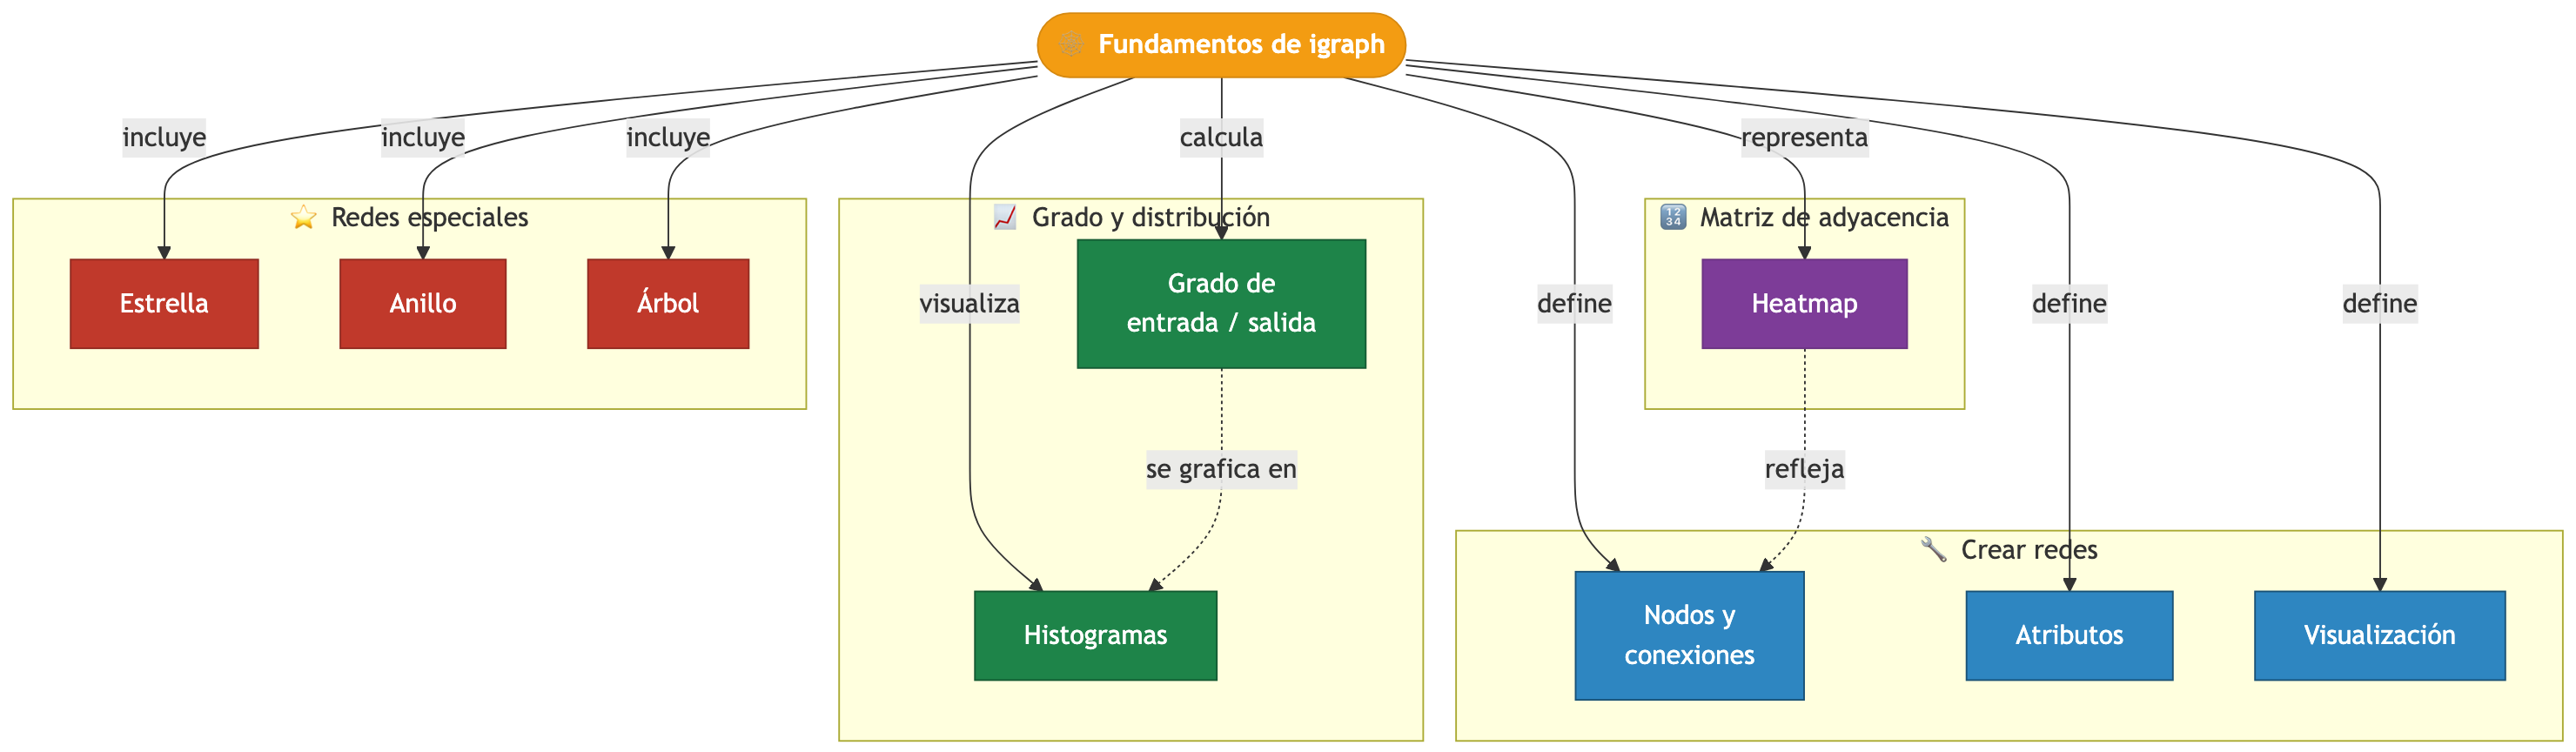
\includegraphics[width=16.34in,height=4.78in]{01-fundamentos-igraph_files/figure-latex/mermaid-figure-1.png}

}

\caption{\label{fig-mapa-cap1}Mapa conceptual del capítulo}

\end{figure}%

\section{Preparación del entorno}\label{preparaciuxf3n-del-entorno}

\begin{Shaded}
\begin{Highlighting}[]
\FunctionTok{library}\NormalTok{(igraph)}
\end{Highlighting}
\end{Shaded}

\begin{tcolorbox}[enhanced jigsaw, colback=white, toprule=.15mm, title=\textcolor{quarto-callout-note-color}{\faInfo}\hspace{0.5em}{📦 Paquete requerido}, titlerule=0mm, colframe=quarto-callout-note-color-frame, breakable, opacitybacktitle=0.6, toptitle=1mm, left=2mm, bottomrule=.15mm, bottomtitle=1mm, arc=.35mm, rightrule=.15mm, leftrule=.75mm, opacityback=0, coltitle=black, colbacktitle=quarto-callout-note-color!10!white]

Si no tienes instalado \texttt{igraph}, ejecuta:

\begin{Shaded}
\begin{Highlighting}[]
\FunctionTok{install.packages}\NormalTok{(}\StringTok{"igraph"}\NormalTok{)}
\end{Highlighting}
\end{Shaded}

\end{tcolorbox}

\section{Crear redes desde cero}\label{crear-redes-desde-cero}

Un \textbf{grafo} (o red) se compone de \textbf{vértices} (nodos) y
\textbf{conexiones} (conexiones entre nodos). En \texttt{igraph},
podemos comenzar creando un grafo vacío y luego añadiendo elementos.

\begin{tcolorbox}[enhanced jigsaw, colback=white, toprule=.15mm, title=\textcolor{quarto-callout-tip-color}{\faLightbulb}\hspace{0.5em}{💡 Concepto clave}, titlerule=0mm, colframe=quarto-callout-tip-color-frame, breakable, opacitybacktitle=0.6, toptitle=1mm, left=2mm, bottomrule=.15mm, bottomtitle=1mm, arc=.35mm, rightrule=.15mm, leftrule=.75mm, opacityback=0, coltitle=black, colbacktitle=quarto-callout-tip-color!10!white]

En \texttt{igraph}, los vértices se acceden con \texttt{V(g)} y las
conexiones con \texttt{E(g)}. Piensa en \texttt{V} de \emph{vertices} y
\texttt{E} de \emph{edges}.

\end{tcolorbox}

\subsection{Paso 1: Grafo vacío}\label{paso-1-grafo-vacuxedo}

\begin{Shaded}
\begin{Highlighting}[]
\CommentTok{\# Crear un grafo dirigido vacío con 5 nodos}
\NormalTok{g }\OtherTok{\textless{}{-}} \FunctionTok{make\_empty\_graph}\NormalTok{(}\AttributeTok{n =} \DecValTok{5}\NormalTok{, }\AttributeTok{directed =} \ConstantTok{TRUE}\NormalTok{)}

\CommentTok{\# Asignar atributos visuales a los nodos}
\FunctionTok{V}\NormalTok{(g)}\SpecialCharTok{$}\NormalTok{color }\OtherTok{\textless{}{-}} \StringTok{"yellow"}

\CommentTok{\# Visualizar}
\FunctionTok{plot}\NormalTok{(g, }
     \AttributeTok{main =} \StringTok{"Red vacía con 5 nodos"}\NormalTok{,}
     \AttributeTok{vertex.size =} \DecValTok{30}\NormalTok{)}
\end{Highlighting}
\end{Shaded}

\begin{figure}[H]

{\centering \pandocbounded{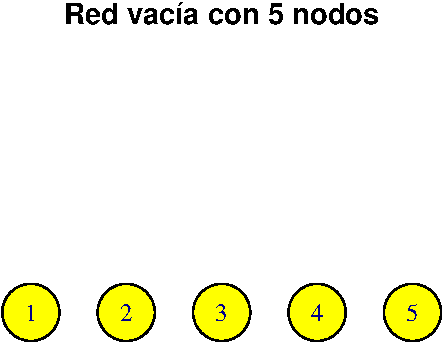
\includegraphics[keepaspectratio]{01-fundamentos-igraph_files/figure-pdf/crear-grafo-vacio-1.pdf}}

}

\caption{Red vacía con 5 nodos y sin conexiones}

\end{figure}%

\subsection{Paso 2: Agregar conexiones}\label{paso-2-agregar-conexiones}

Las conexiones se agregan como un vector de pares:
\texttt{c(origen1,\ destino1,\ origen2,\ destino2,\ ...)}.

\begin{Shaded}
\begin{Highlighting}[]
\CommentTok{\# Agregar conexiones: 1→2, 1→3, 2→4, 3→4, 4→5}
\NormalTok{g }\OtherTok{\textless{}{-}} \FunctionTok{add\_edges}\NormalTok{(g, }\FunctionTok{c}\NormalTok{(}\DecValTok{1}\NormalTok{,}\DecValTok{2}\NormalTok{, }\DecValTok{1}\NormalTok{,}\DecValTok{3}\NormalTok{, }\DecValTok{2}\NormalTok{,}\DecValTok{4}\NormalTok{, }\DecValTok{3}\NormalTok{,}\DecValTok{4}\NormalTok{, }\DecValTok{4}\NormalTok{,}\DecValTok{5}\NormalTok{))}

\FunctionTok{plot}\NormalTok{(g, }
     \AttributeTok{main =} \StringTok{"Red con conexiones agregadas"}\NormalTok{,}
     \AttributeTok{vertex.size =} \DecValTok{30}\NormalTok{,}
     \AttributeTok{edge.arrow.size =} \FloatTok{0.6}\NormalTok{)}
\end{Highlighting}
\end{Shaded}

\begin{figure}[H]

{\centering \pandocbounded{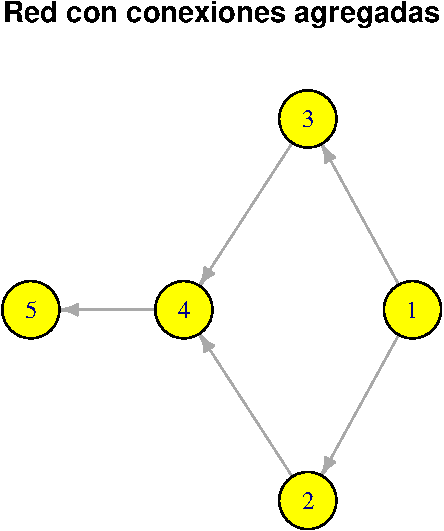
\includegraphics[keepaspectratio]{01-fundamentos-igraph_files/figure-pdf/agregar-conexiones-1.pdf}}

}

\caption{Red con conexiones agregadas manualmente}

\end{figure}%

\subsection{Paso 3: Agregar nodos con
atributos}\label{paso-3-agregar-nodos-con-atributos}

\begin{Shaded}
\begin{Highlighting}[]
\CommentTok{\# Agregar un nodo nuevo con color rojo}
\NormalTok{g }\OtherTok{\textless{}{-}} \FunctionTok{add\_vertices}\NormalTok{(g, }\DecValTok{1}\NormalTok{, }\AttributeTok{color =} \StringTok{"red"}\NormalTok{)}

\CommentTok{\# Conectar el nuevo nodo (nodo 6)}
\NormalTok{g }\OtherTok{\textless{}{-}} \FunctionTok{add\_edges}\NormalTok{(g, }\FunctionTok{c}\NormalTok{(}\DecValTok{3}\NormalTok{,}\DecValTok{6}\NormalTok{, }\DecValTok{6}\NormalTok{,}\DecValTok{5}\NormalTok{))}

\FunctionTok{plot}\NormalTok{(g, }
     \AttributeTok{main =} \StringTok{"Nodo rojo y nuevas conexiones"}\NormalTok{,}
     \AttributeTok{vertex.size =} \DecValTok{30}\NormalTok{,}
     \AttributeTok{edge.arrow.size =} \FloatTok{0.6}\NormalTok{)}
\end{Highlighting}
\end{Shaded}

\begin{figure}[H]

{\centering \pandocbounded{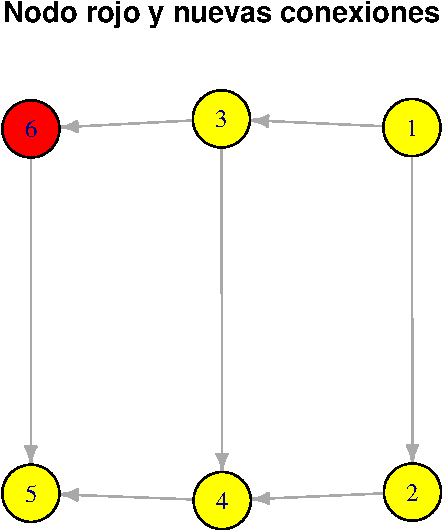
\includegraphics[keepaspectratio]{01-fundamentos-igraph_files/figure-pdf/agregar-nodo-1.pdf}}

}

\caption{Nodo rojo agregado con nuevas conexiones}

\end{figure}%

\subsection{Paso 4: Nombrar los nodos}\label{paso-4-nombrar-los-nodos}

\begin{Shaded}
\begin{Highlighting}[]
\CommentTok{\# Asignar nombres a los vértices}
\FunctionTok{V}\NormalTok{(g)}\SpecialCharTok{$}\NormalTok{name }\OtherTok{\textless{}{-}}\NormalTok{ LETTERS[}\DecValTok{1}\SpecialCharTok{:}\DecValTok{6}\NormalTok{]}

\FunctionTok{plot}\NormalTok{(g, }
     \AttributeTok{main =} \StringTok{"Nodos con nombres A–F"}\NormalTok{,}
     \AttributeTok{vertex.size =} \DecValTok{30}\NormalTok{,}
     \AttributeTok{edge.arrow.size =} \FloatTok{0.6}\NormalTok{)}
\end{Highlighting}
\end{Shaded}

\begin{figure}[H]

{\centering \pandocbounded{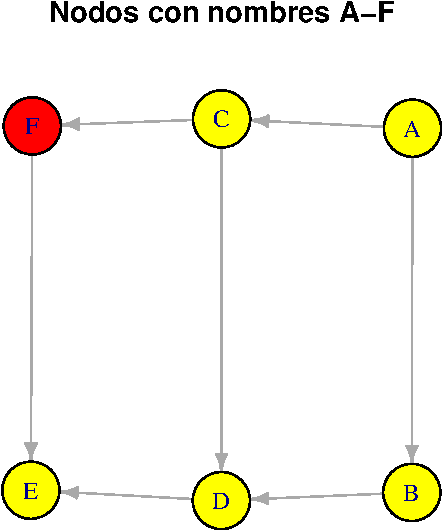
\includegraphics[keepaspectratio]{01-fundamentos-igraph_files/figure-pdf/renombrar-nodos-1.pdf}}

}

\caption{Red con nodos etiquetados de A a F}

\end{figure}%

\subsection{Paso 5: Modificar
conexiones}\label{paso-5-modificar-conexiones}

\begin{Shaded}
\begin{Highlighting}[]
\CommentTok{\# Eliminar la segunda conexión (A→C) y agregar C→A}
\NormalTok{g }\OtherTok{\textless{}{-}} \FunctionTok{delete\_edges}\NormalTok{(g, }\DecValTok{2}\NormalTok{)}
\NormalTok{g }\OtherTok{\textless{}{-}} \FunctionTok{add\_edges}\NormalTok{(g, }\FunctionTok{c}\NormalTok{(}\DecValTok{3}\NormalTok{, }\DecValTok{1}\NormalTok{))  }\CommentTok{\# C → A}

\FunctionTok{plot}\NormalTok{(g, }
     \AttributeTok{main =} \StringTok{"Cambio en dirección de conexión"}\NormalTok{,}
     \AttributeTok{vertex.size =} \DecValTok{30}\NormalTok{,}
     \AttributeTok{edge.arrow.size =} \FloatTok{0.6}\NormalTok{)}
\end{Highlighting}
\end{Shaded}

\begin{figure}[H]

{\centering \pandocbounded{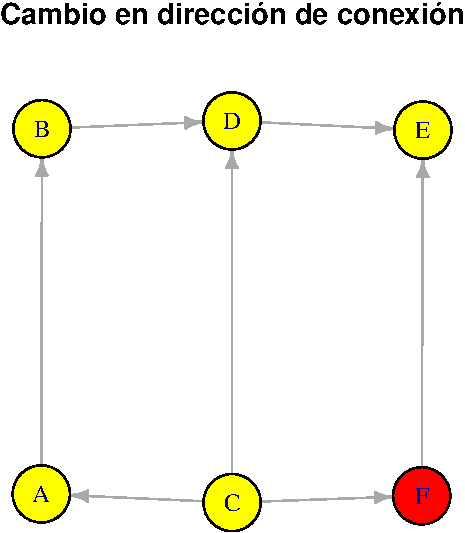
\includegraphics[keepaspectratio]{01-fundamentos-igraph_files/figure-pdf/modificar-conexiones-1.pdf}}

}

\caption{Red con dirección de conexión modificada}

\end{figure}%

\begin{tcolorbox}[enhanced jigsaw, colback=white, toprule=.15mm, title=\textcolor{quarto-callout-warning-color}{\faExclamationTriangle}\hspace{0.5em}{⚠️ Error frecuente}, titlerule=0mm, colframe=quarto-callout-warning-color-frame, breakable, opacitybacktitle=0.6, toptitle=1mm, left=2mm, bottomrule=.15mm, bottomtitle=1mm, arc=.35mm, rightrule=.15mm, leftrule=.75mm, opacityback=0, coltitle=black, colbacktitle=quarto-callout-warning-color!10!white]

Cuando eliminas conexiones con \texttt{delete\_edges()}, los
\textbf{índices se reorganizan}. Si eliminas la conexión 2, la que antes
era la 3 ahora es la 2. Siempre verifica con \texttt{E(g)} después de
eliminar.

\end{tcolorbox}

\section{grado (degree) y distribución de grado (degree) \{\#sec-grado
(degree)-basico\}}\label{grado-degree-y-distribuciuxf3n-de-grado-degree-sec-grado-degree-basico}

El \textbf{grado (degree)} de un nodo es el número de conexiones que
tiene. En redes dirigidas, distinguimos entre grado (degree) de entrada
(\emph{in-degree}) y de salida (\emph{out-degree}).

\subsection{grado (degree) total}

\begin{Shaded}
\begin{Highlighting}[]
\CommentTok{\# grado (degree) total de cada nodo}
\FunctionTok{degree}\NormalTok{(g)}
\end{Highlighting}
\end{Shaded}

\begin{verbatim}
A B C D E F 
2 2 3 3 2 2 
\end{verbatim}

\subsection{grado (degree) de entrada}

\begin{Shaded}
\begin{Highlighting}[]
\CommentTok{\# ¿Cuántas conexiones llegan a cada nodo?}
\FunctionTok{degree}\NormalTok{(g, }\AttributeTok{mode =} \StringTok{"in"}\NormalTok{)}
\end{Highlighting}
\end{Shaded}

\begin{verbatim}
A B C D E F 
1 1 0 2 2 1 
\end{verbatim}

\subsection{grado (degree) de salida}

\begin{Shaded}
\begin{Highlighting}[]
\CommentTok{\# ¿Cuántas conexiones salen de cada nodo?}
\FunctionTok{degree}\NormalTok{(g, }\AttributeTok{mode =} \StringTok{"out"}\NormalTok{)}
\end{Highlighting}
\end{Shaded}

\begin{verbatim}
A B C D E F 
1 1 3 1 0 1 
\end{verbatim}

\subsection{Visualizar el grado
(degree)}\label{visualizar-el-grado-degree}

\begin{Shaded}
\begin{Highlighting}[]
\FunctionTok{plot}\NormalTok{(g, }
     \AttributeTok{layout =} \FunctionTok{layout\_nicely}\NormalTok{(g),}
     \AttributeTok{vertex.size =} \FunctionTok{degree}\NormalTok{(g, }\AttributeTok{mode =} \StringTok{"in"}\NormalTok{) }\SpecialCharTok{*} \DecValTok{10} \SpecialCharTok{+} \DecValTok{10}\NormalTok{,}
     \AttributeTok{vertex.label.dist =} \FloatTok{0.5}\NormalTok{,}
     \AttributeTok{edge.arrow.size =} \FloatTok{0.5}\NormalTok{,}
     \AttributeTok{main =} \StringTok{"Tamaño proporcional al grado (degree) de entrada"}\NormalTok{)}
\end{Highlighting}
\end{Shaded}

\pandocbounded{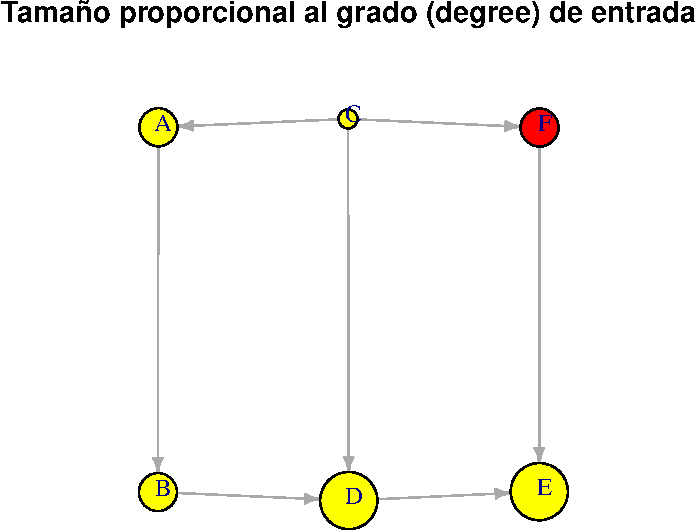
\includegraphics[keepaspectratio]{01-fundamentos-igraph_files/figure-pdf/fig-tamano-grado (degree)-1.pdf}}\{\#fig-tamano-grado
(degree) fig-alt=`Red donde los nodos más grandes reciben más
conexiones'\}

\begin{Shaded}
\begin{Highlighting}[]
\FunctionTok{hist}\NormalTok{(}\FunctionTok{degree}\NormalTok{(g), }
     \AttributeTok{col =} \StringTok{"salmon"}\NormalTok{, }
     \AttributeTok{main =} \StringTok{"Histograma del grado (degree)"}\NormalTok{,}
     \AttributeTok{xlab =} \StringTok{"grado (degree)"}\NormalTok{,}
     \AttributeTok{ylab =} \StringTok{"Frecuencia"}\NormalTok{,}
     \AttributeTok{border =} \StringTok{"white"}\NormalTok{)}
\end{Highlighting}
\end{Shaded}

\pandocbounded{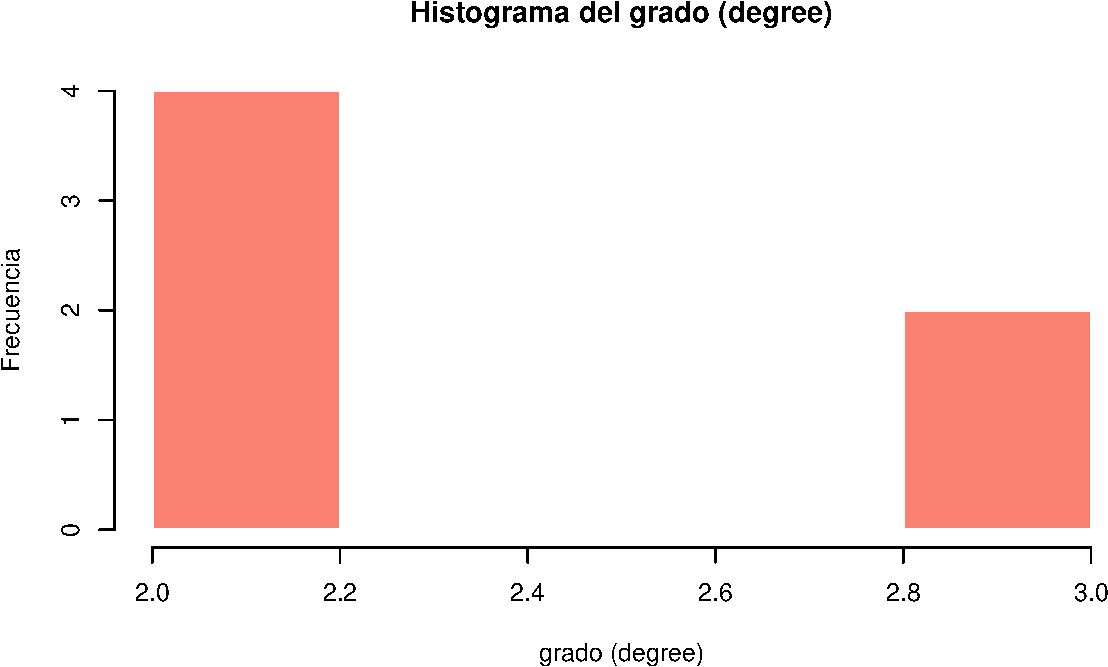
\includegraphics[keepaspectratio]{01-fundamentos-igraph_files/figure-pdf/fig-histograma-grado (degree)-1.pdf}}\{\#fig-histograma-grado
(degree) fig-alt=`Histograma que muestra la frecuencia de cada valor de
grado (degree)'\}

\section{Matriz de adyacencia}\label{sec-matriz-adyacencia}

La \textbf{matriz de adyacencia} es una representación numérica de la
red: un 1 en la posición \((i,j)\) indica que existe una conexión del
nodo \(i\) al nodo \(j\).

\[
A_{ij} = \begin{cases} 1 & \text{si existe conexión de } i \text{ a } j \\ 0 & \text{en otro caso} \end{cases}
\]

\begin{Shaded}
\begin{Highlighting}[]
\CommentTok{\# Obtener la matriz de adyacencia}
\NormalTok{adj\_mat }\OtherTok{\textless{}{-}} \FunctionTok{as.matrix}\NormalTok{(}\FunctionTok{get.adjacency}\NormalTok{(g))}

\CommentTok{\# Mostrar como tabla}
\NormalTok{knitr}\SpecialCharTok{::}\FunctionTok{kable}\NormalTok{(adj\_mat, }\AttributeTok{caption =} \StringTok{"Matriz de adyacencia de la red"}\NormalTok{)}
\end{Highlighting}
\end{Shaded}

\begin{longtable}[]{@{}lrrrrrr@{}}
\caption{Matriz de adyacencia de la red}\tabularnewline
\toprule\noalign{}
& A & B & C & D & E & F \\
\midrule\noalign{}
\endfirsthead
\toprule\noalign{}
& A & B & C & D & E & F \\
\midrule\noalign{}
\endhead
\bottomrule\noalign{}
\endlastfoot
A & 0 & 1 & 0 & 0 & 0 & 0 \\
B & 0 & 0 & 0 & 1 & 0 & 0 \\
C & 1 & 0 & 0 & 1 & 0 & 1 \\
D & 0 & 0 & 0 & 0 & 1 & 0 \\
E & 0 & 0 & 0 & 0 & 0 & 0 \\
F & 0 & 0 & 0 & 0 & 1 & 0 \\
\end{longtable}

\begin{Shaded}
\begin{Highlighting}[]
\FunctionTok{heatmap}\NormalTok{(adj\_mat, }
        \AttributeTok{Rowv =} \ConstantTok{NA}\NormalTok{, }\AttributeTok{Colv =} \ConstantTok{NA}\NormalTok{, }
        \AttributeTok{col =} \FunctionTok{c}\NormalTok{(}\StringTok{"white"}\NormalTok{, }\StringTok{"steelblue"}\NormalTok{),}
        \AttributeTok{main =} \StringTok{"Mapa de calor — Matriz de adyacencia"}\NormalTok{,}
        \AttributeTok{scale =} \StringTok{"none"}\NormalTok{)}
\end{Highlighting}
\end{Shaded}

\begin{figure}[H]

\centering{

\pandocbounded{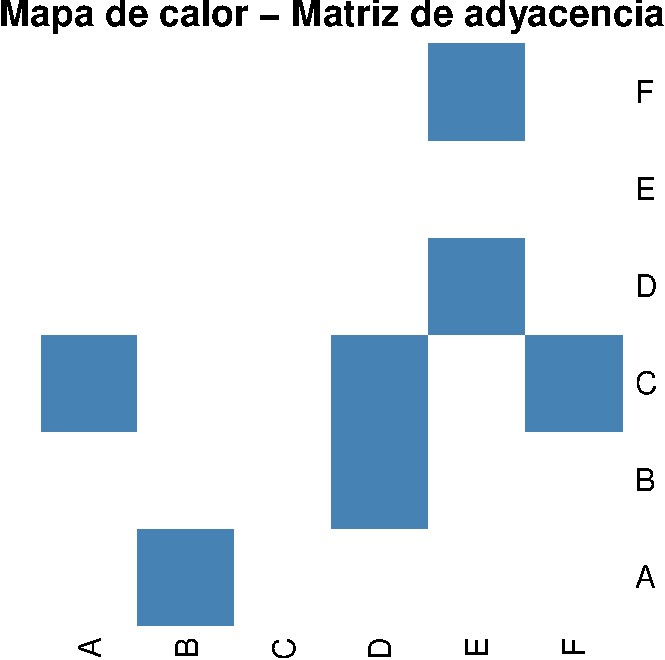
\includegraphics[keepaspectratio]{01-fundamentos-igraph_files/figure-pdf/fig-heatmap-adj-1.pdf}}

}

\caption{\label{fig-heatmap-adj}Mapa de calor de la matriz de
adyacencia}

\end{figure}%

\begin{tcolorbox}[enhanced jigsaw, colback=white, toprule=.15mm, title=\textcolor{quarto-callout-tip-color}{\faLightbulb}\hspace{0.5em}{💡 Concepto clave}, titlerule=0mm, colframe=quarto-callout-tip-color-frame, breakable, opacitybacktitle=0.6, toptitle=1mm, left=2mm, bottomrule=.15mm, bottomtitle=1mm, arc=.35mm, rightrule=.15mm, leftrule=.75mm, opacityback=0, coltitle=black, colbacktitle=quarto-callout-tip-color!10!white]

En una red \textbf{no dirigida}, la matriz de adyacencia es
\textbf{simétrica} (\(A_{ij} = A_{ji}\)). En una red dirigida, no
necesariamente lo es. Verifica esto convirtiendo la red con
\texttt{as.undirected(g)}.

\end{tcolorbox}

\section{Redes especiales}\label{sec-redes-especiales}

\texttt{igraph} incluye funciones para crear topologías clásicas que
aparecen frecuentemente en la teoría de redes.

\subsection{Estrella}

\begin{Shaded}
\begin{Highlighting}[]
\FunctionTok{plot}\NormalTok{(}\FunctionTok{make\_star}\NormalTok{(}\DecValTok{10}\NormalTok{), }
     \AttributeTok{vertex.color =} \FunctionTok{c}\NormalTok{(}\StringTok{"tomato"}\NormalTok{, }\FunctionTok{rep}\NormalTok{(}\StringTok{"gold"}\NormalTok{, }\DecValTok{9}\NormalTok{)),}
     \AttributeTok{vertex.size =} \DecValTok{20}\NormalTok{,}
     \AttributeTok{main =} \StringTok{"Red estrella"}\NormalTok{)}
\end{Highlighting}
\end{Shaded}

\begin{figure}[H]

\centering{

\pandocbounded{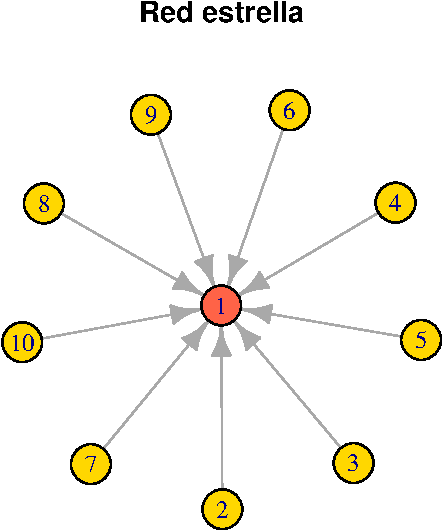
\includegraphics[keepaspectratio]{01-fundamentos-igraph_files/figure-pdf/fig-red-estrella-1.pdf}}

}

\caption{\label{fig-red-estrella}Red tipo estrella con 10 nodos}

\end{figure}%

\subsection{Anillo}

\begin{Shaded}
\begin{Highlighting}[]
\FunctionTok{plot}\NormalTok{(}\FunctionTok{make\_ring}\NormalTok{(}\DecValTok{10}\NormalTok{), }
     \AttributeTok{vertex.color =} \StringTok{"skyblue"}\NormalTok{,}
     \AttributeTok{vertex.size =} \DecValTok{20}\NormalTok{,}
     \AttributeTok{main =} \StringTok{"Red anillo"}\NormalTok{)}
\end{Highlighting}
\end{Shaded}

\begin{figure}[H]

\centering{

\pandocbounded{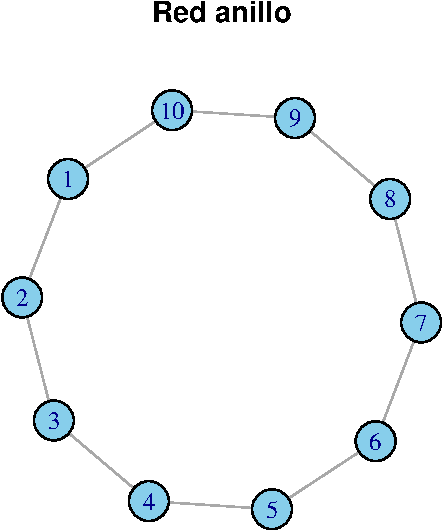
\includegraphics[keepaspectratio]{01-fundamentos-igraph_files/figure-pdf/fig-red-anillo-1.pdf}}

}

\caption{\label{fig-red-anillo}Red tipo anillo con 10 nodos}

\end{figure}%

\subsection{Árbol binario}

\begin{Shaded}
\begin{Highlighting}[]
\FunctionTok{plot}\NormalTok{(}\FunctionTok{make\_tree}\NormalTok{(}\DecValTok{15}\NormalTok{, }\AttributeTok{children =} \DecValTok{2}\NormalTok{), }
     \AttributeTok{vertex.color =} \StringTok{"lightgreen"}\NormalTok{,}
     \AttributeTok{vertex.size =} \DecValTok{15}\NormalTok{,}
     \AttributeTok{layout =}\NormalTok{ layout\_as\_tree,}
     \AttributeTok{main =} \StringTok{"Árbol binario"}\NormalTok{)}
\end{Highlighting}
\end{Shaded}

\begin{figure}[H]

\centering{

\pandocbounded{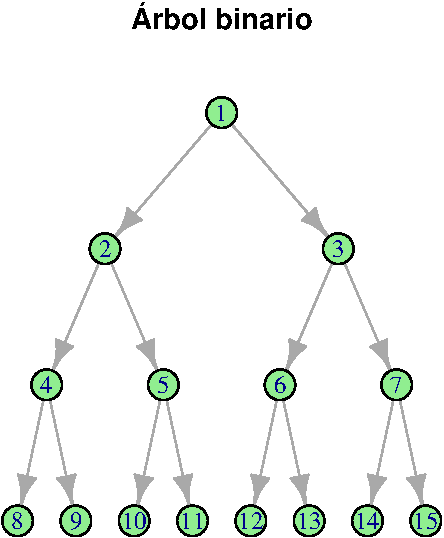
\includegraphics[keepaspectratio]{01-fundamentos-igraph_files/figure-pdf/fig-red-arbol-1.pdf}}

}

\caption{\label{fig-red-arbol}Árbol binario con 15 nodos}

\end{figure}%

\subsection{Lattice}

\begin{Shaded}
\begin{Highlighting}[]
\FunctionTok{plot}\NormalTok{(}\FunctionTok{make\_lattice}\NormalTok{(}\FunctionTok{c}\NormalTok{(}\DecValTok{4}\NormalTok{, }\DecValTok{4}\NormalTok{)), }
     \AttributeTok{vertex.color =} \StringTok{"plum"}\NormalTok{,}
     \AttributeTok{vertex.size =} \DecValTok{20}\NormalTok{,}
     \AttributeTok{main =} \StringTok{"Lattice 4×4"}\NormalTok{)}
\end{Highlighting}
\end{Shaded}

\begin{figure}[H]

\centering{

\pandocbounded{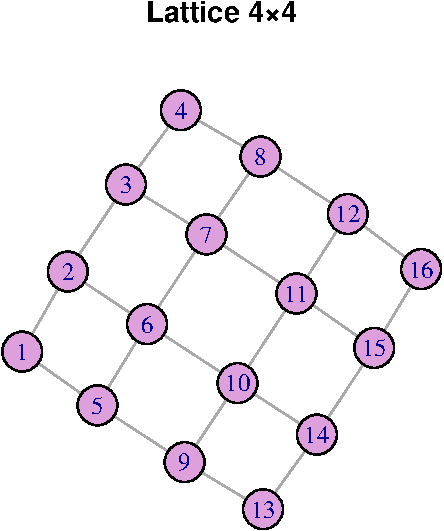
\includegraphics[keepaspectratio]{01-fundamentos-igraph_files/figure-pdf/fig-red-lattice-1.pdf}}

}

\caption{\label{fig-red-lattice}Red tipo rejilla (lattice) de 4×4}

\end{figure}%

\section{Ejercicios}\label{ejercicios}

\subsection*{Ejercicios resueltos}\label{ejercicios-resueltos}
\addcontentsline{toc}{subsection}{Ejercicios resueltos}

\textbf{Ejercicio resuelto 1:} Crea una red no dirigida de 7 nodos con
colores aleatorios de una paleta, conéctalos formando una cadena
(\emph{path}), y visualiza el resultado.

\begin{tcolorbox}[enhanced jigsaw, colback=white, toprule=.15mm, title=\textcolor{quarto-callout-tip-color}{\faLightbulb}\hspace{0.5em}{📝 Solución}, titlerule=0mm, colframe=quarto-callout-tip-color-frame, breakable, opacitybacktitle=0.6, toptitle=1mm, left=2mm, bottomrule=.15mm, bottomtitle=1mm, arc=.35mm, rightrule=.15mm, leftrule=.75mm, opacityback=0, coltitle=black, colbacktitle=quarto-callout-tip-color!10!white]

\textbf{Paso 1:} Crear el grafo tipo cadena y asignar colores.

\begin{Shaded}
\begin{Highlighting}[]
\FunctionTok{set.seed}\NormalTok{(}\DecValTok{42}\NormalTok{)}

\CommentTok{\# Crear cadena de 7 nodos}
\CommentTok{\#g\_cadena \textless{}{-} make\_graph(\textasciitilde{} 1{-}2{-}3{-}4{-}5{-}6{-}7, directed = FALSE)}
\NormalTok{g\_cadena }\OtherTok{\textless{}{-}} \FunctionTok{graph\_from\_literal}\NormalTok{(}\DecValTok{1{-}2{-}3{-}4{-}5{-}6{-}7}\NormalTok{)}
\CommentTok{\# Asignar colores aleatorios de una paleta}
\NormalTok{paleta }\OtherTok{\textless{}{-}} \FunctionTok{c}\NormalTok{(}\StringTok{"tomato"}\NormalTok{, }\StringTok{"gold"}\NormalTok{, }\StringTok{"skyblue"}\NormalTok{, }\StringTok{"lightgreen"}\NormalTok{, }\StringTok{"plum"}\NormalTok{, }\StringTok{"salmon"}\NormalTok{, }\StringTok{"steelblue"}\NormalTok{)}
\FunctionTok{V}\NormalTok{(g\_cadena)}\SpecialCharTok{$}\NormalTok{color }\OtherTok{\textless{}{-}} \FunctionTok{sample}\NormalTok{(paleta, }\DecValTok{7}\NormalTok{)}
\FunctionTok{V}\NormalTok{(g\_cadena)}\SpecialCharTok{$}\NormalTok{name }\OtherTok{\textless{}{-}} \FunctionTok{paste0}\NormalTok{(}\StringTok{"N"}\NormalTok{, }\DecValTok{1}\SpecialCharTok{:}\DecValTok{7}\NormalTok{)}
\end{Highlighting}
\end{Shaded}

\textbf{Paso 2:} Visualizar la red.

\begin{Shaded}
\begin{Highlighting}[]
\FunctionTok{plot}\NormalTok{(g\_cadena, }
     \AttributeTok{vertex.size =} \DecValTok{30}\NormalTok{, }
     \AttributeTok{main =} \StringTok{"Red tipo cadena (path)"}\NormalTok{)}
\end{Highlighting}
\end{Shaded}

\begin{figure}[H]

\centering{

\pandocbounded{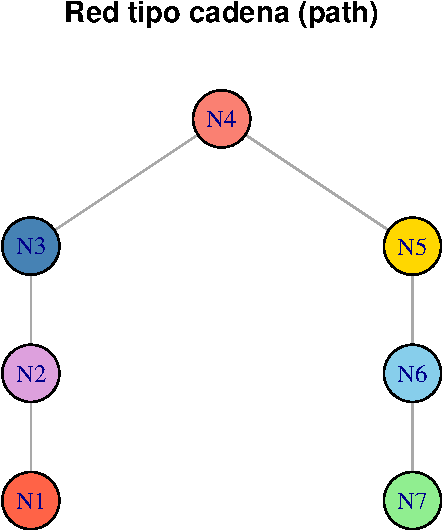
\includegraphics[keepaspectratio]{01-fundamentos-igraph_files/figure-pdf/fig-ej-resuelto-1-1.pdf}}

}

\caption{\label{fig-ej-resuelto-1}Red tipo cadena con 7 nodos y colores
aleatorios}

\end{figure}%

\textbf{Paso 3:} Verificar propiedades.

\begin{Shaded}
\begin{Highlighting}[]
\FunctionTok{cat}\NormalTok{(}\StringTok{"Número de nodos:"}\NormalTok{, }\FunctionTok{vcount}\NormalTok{(g\_cadena), }\StringTok{"}\SpecialCharTok{\textbackslash{}n}\StringTok{"}\NormalTok{)}
\end{Highlighting}
\end{Shaded}

\begin{verbatim}
Número de nodos: 7 
\end{verbatim}

\begin{Shaded}
\begin{Highlighting}[]
\FunctionTok{cat}\NormalTok{(}\StringTok{"Número de conexiones:"}\NormalTok{, }\FunctionTok{ecount}\NormalTok{(g\_cadena), }\StringTok{"}\SpecialCharTok{\textbackslash{}n}\StringTok{"}\NormalTok{)}
\end{Highlighting}
\end{Shaded}

\begin{verbatim}
Número de conexiones: 6 
\end{verbatim}

\begin{Shaded}
\begin{Highlighting}[]
\FunctionTok{cat}\NormalTok{(}\StringTok{"grado (degree) de cada nodo:"}\NormalTok{, }\FunctionTok{degree}\NormalTok{(g\_cadena), }\StringTok{"}\SpecialCharTok{\textbackslash{}n}\StringTok{"}\NormalTok{)}
\end{Highlighting}
\end{Shaded}

\begin{verbatim}
grado (degree) de cada nodo: 1 2 2 2 2 2 1 
\end{verbatim}

\begin{Shaded}
\begin{Highlighting}[]
\FunctionTok{cat}\NormalTok{(}\StringTok{"¿Es conexa?"}\NormalTok{, }\FunctionTok{is\_connected}\NormalTok{(g\_cadena), }\StringTok{"}\SpecialCharTok{\textbackslash{}n}\StringTok{"}\NormalTok{)}
\end{Highlighting}
\end{Shaded}

\begin{verbatim}
¿Es conexa? TRUE 
\end{verbatim}

\textbf{Interpretación:} La cadena tiene 7 nodos y 6 conexiones. Los
nodos extremos tienen grado (degree) 1 y los internos grado (degree) 2.
La red es conexa (todos los nodos se pueden alcanzar entre sí).

\end{tcolorbox}

\begin{center}\rule{0.5\linewidth}{0.5pt}\end{center}

\textbf{Ejercicio resuelto 2:} Construye manualmente una red donde los
nodos representen 5 ciudades mexicanas y las conexiones indiquen si
comparten frontera estatal. Muestra la matriz de adyacencia.

\begin{tcolorbox}[enhanced jigsaw, colback=white, toprule=.15mm, title=\textcolor{quarto-callout-tip-color}{\faLightbulb}\hspace{0.5em}{📝 Solución}, titlerule=0mm, colframe=quarto-callout-tip-color-frame, breakable, opacitybacktitle=0.6, toptitle=1mm, left=2mm, bottomrule=.15mm, bottomtitle=1mm, arc=.35mm, rightrule=.15mm, leftrule=.75mm, opacityback=0, coltitle=black, colbacktitle=quarto-callout-tip-color!10!white]

\textbf{Paso 1:} Definir las ciudades y sus conexiones fronterizas.

\begin{Shaded}
\begin{Highlighting}[]
\CommentTok{\# Crear la red}
\NormalTok{ciudades }\OtherTok{\textless{}{-}} \FunctionTok{graph\_from\_literal}\NormalTok{(}
\NormalTok{  Querétaro }\SpecialCharTok{{-}{-}}\NormalTok{ Guanajuato,}
\NormalTok{  Querétaro }\SpecialCharTok{{-}{-}} \StringTok{"San Luis Potosí"}\NormalTok{,}
\NormalTok{  Querétaro }\SpecialCharTok{{-}{-}}\NormalTok{ Hidalgo,}
\NormalTok{  Guanajuato }\SpecialCharTok{{-}{-}} \StringTok{"San Luis Potosí"}\NormalTok{,}
\NormalTok{  Hidalgo }\SpecialCharTok{{-}{-}} \StringTok{"Estado de México"}
\NormalTok{)}

\FunctionTok{V}\NormalTok{(ciudades)}\SpecialCharTok{$}\NormalTok{color }\OtherTok{\textless{}{-}} \StringTok{"gold"}
\FunctionTok{V}\NormalTok{(ciudades)}\SpecialCharTok{$}\NormalTok{size }\OtherTok{\textless{}{-}} \DecValTok{25}
\end{Highlighting}
\end{Shaded}

\textbf{Paso 2:} Visualizar y mostrar la matriz.

\begin{Shaded}
\begin{Highlighting}[]
\FunctionTok{plot}\NormalTok{(ciudades, }
     \AttributeTok{vertex.label.cex =} \FloatTok{0.8}\NormalTok{,}
     \AttributeTok{main =} \StringTok{"Red de vecindad entre estados"}\NormalTok{)}
\end{Highlighting}
\end{Shaded}

\begin{figure}[H]

\centering{

\pandocbounded{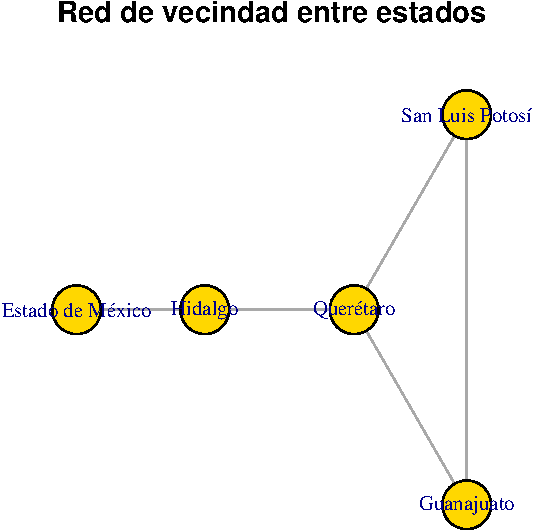
\includegraphics[keepaspectratio]{01-fundamentos-igraph_files/figure-pdf/fig-ej-resuelto-2-1.pdf}}

}

\caption{\label{fig-ej-resuelto-2}Red de ciudades que comparten frontera
estatal}

\end{figure}%

\begin{Shaded}
\begin{Highlighting}[]
\NormalTok{knitr}\SpecialCharTok{::}\FunctionTok{kable}\NormalTok{(}
  \FunctionTok{as.matrix}\NormalTok{(}\FunctionTok{get.adjacency}\NormalTok{(ciudades)),}
  \AttributeTok{caption =} \StringTok{"Matriz de adyacencia de la red de estados"}
\NormalTok{)}
\end{Highlighting}
\end{Shaded}

\begin{longtable}[]{@{}
  >{\raggedright\arraybackslash}p{(\linewidth - 10\tabcolsep) * \real{0.2152}}
  >{\raggedleft\arraybackslash}p{(\linewidth - 10\tabcolsep) * \real{0.1266}}
  >{\raggedleft\arraybackslash}p{(\linewidth - 10\tabcolsep) * \real{0.1392}}
  >{\raggedleft\arraybackslash}p{(\linewidth - 10\tabcolsep) * \real{0.2025}}
  >{\raggedleft\arraybackslash}p{(\linewidth - 10\tabcolsep) * \real{0.1013}}
  >{\raggedleft\arraybackslash}p{(\linewidth - 10\tabcolsep) * \real{0.2152}}@{}}
\caption{Matriz de adyacencia de la red de estados}\tabularnewline
\toprule\noalign{}
\begin{minipage}[b]{\linewidth}\raggedright
\end{minipage} & \begin{minipage}[b]{\linewidth}\raggedleft
Querétaro
\end{minipage} & \begin{minipage}[b]{\linewidth}\raggedleft
Guanajuato
\end{minipage} & \begin{minipage}[b]{\linewidth}\raggedleft
San Luis Potosí
\end{minipage} & \begin{minipage}[b]{\linewidth}\raggedleft
Hidalgo
\end{minipage} & \begin{minipage}[b]{\linewidth}\raggedleft
Estado de México
\end{minipage} \\
\midrule\noalign{}
\endfirsthead
\toprule\noalign{}
\begin{minipage}[b]{\linewidth}\raggedright
\end{minipage} & \begin{minipage}[b]{\linewidth}\raggedleft
Querétaro
\end{minipage} & \begin{minipage}[b]{\linewidth}\raggedleft
Guanajuato
\end{minipage} & \begin{minipage}[b]{\linewidth}\raggedleft
San Luis Potosí
\end{minipage} & \begin{minipage}[b]{\linewidth}\raggedleft
Hidalgo
\end{minipage} & \begin{minipage}[b]{\linewidth}\raggedleft
Estado de México
\end{minipage} \\
\midrule\noalign{}
\endhead
\bottomrule\noalign{}
\endlastfoot
Querétaro & 0 & 1 & 1 & 1 & 0 \\
Guanajuato & 1 & 0 & 1 & 0 & 0 \\
San Luis Potosí & 1 & 1 & 0 & 0 & 0 \\
Hidalgo & 1 & 0 & 0 & 0 & 1 \\
Estado de México & 0 & 0 & 0 & 1 & 0 \\
\end{longtable}

\textbf{Interpretación:} Querétaro es el nodo más conectado (grado
(degree) 3) porque comparte frontera con tres estados. La matriz es
simétrica porque la red es no dirigida.

\end{tcolorbox}

\subsection*{Ejercicios con pistas}\label{ejercicios-con-pistas}
\addcontentsline{toc}{subsection}{Ejercicios con pistas}

\textbf{Ejercicio 1:} Crea una red vacía de 7 nodos no dirigidos. Agrega
conexiones para formar un triángulo entre los nodos 1, 2 y 3, y otro
triángulo entre 5, 6 y 7. Conecta ambos triángulos con una conexión
entre 3 y 5. Visualiza el resultado y calcula el grado (degree) de cada
nodo.

\begin{tcolorbox}[enhanced jigsaw, colback=white, toprule=.15mm, title=\textcolor{quarto-callout-note-color}{\faInfo}\hspace{0.5em}{💡 Pista 1}, titlerule=0mm, colframe=quarto-callout-note-color-frame, breakable, opacitybacktitle=0.6, toptitle=1mm, left=2mm, bottomrule=.15mm, bottomtitle=1mm, arc=.35mm, rightrule=.15mm, leftrule=.75mm, opacityback=0, coltitle=black, colbacktitle=quarto-callout-note-color!10!white]

Usa \texttt{make\_empty\_graph(n\ =\ 7,\ directed\ =\ FALSE)} y luego
\texttt{add\_edges()} con el vector de pares.

\end{tcolorbox}

\begin{tcolorbox}[enhanced jigsaw, colback=white, toprule=.15mm, title=\textcolor{quarto-callout-note-color}{\faInfo}\hspace{0.5em}{💡 Pista 2}, titlerule=0mm, colframe=quarto-callout-note-color-frame, breakable, opacitybacktitle=0.6, toptitle=1mm, left=2mm, bottomrule=.15mm, bottomtitle=1mm, arc=.35mm, rightrule=.15mm, leftrule=.75mm, opacityback=0, coltitle=black, colbacktitle=quarto-callout-note-color!10!white]

El vector de conexiones sería:
\texttt{c(1,2,\ 2,3,\ 1,3,\ 5,6,\ 6,7,\ 5,7,\ 3,5)}. Son 7 conexiones en
total.

\end{tcolorbox}

\begin{tcolorbox}[enhanced jigsaw, colback=white, toprule=.15mm, title=\textcolor{quarto-callout-note-color}{\faInfo}\hspace{0.5em}{💡 Pista 3 --- Pseudocódigo}, titlerule=0mm, colframe=quarto-callout-note-color-frame, breakable, opacitybacktitle=0.6, toptitle=1mm, left=2mm, bottomrule=.15mm, bottomtitle=1mm, arc=.35mm, rightrule=.15mm, leftrule=.75mm, opacityback=0, coltitle=black, colbacktitle=quarto-callout-note-color!10!white]

\begin{verbatim}
1. g <- make_empty_graph(7, directed = FALSE)
2. g <- add_edges(g, c(1,2, 2,3, ...))
3. plot(g)
4. degree(g)
\end{verbatim}

\end{tcolorbox}

\begin{center}\rule{0.5\linewidth}{0.5pt}\end{center}

\textbf{Ejercicio 2:} Genera un \texttt{make\_tree()} con 3 hijos por
nodo y profundidad suficiente para tener al menos 40 nodos. ¿Cuántos
nodos tiene exactamente? ¿Cuántas hojas (nodos con grado (degree) 1)?

\begin{tcolorbox}[enhanced jigsaw, colback=white, toprule=.15mm, title=\textcolor{quarto-callout-note-color}{\faInfo}\hspace{0.5em}{💡 Pista 1}, titlerule=0mm, colframe=quarto-callout-note-color-frame, breakable, opacitybacktitle=0.6, toptitle=1mm, left=2mm, bottomrule=.15mm, bottomtitle=1mm, arc=.35mm, rightrule=.15mm, leftrule=.75mm, opacityback=0, coltitle=black, colbacktitle=quarto-callout-note-color!10!white]

En \texttt{make\_tree(n,\ children)}, \texttt{n} es el número total de
nodos. Un árbol con 3 hijos y \texttt{n\ =\ 40} tendrá exactamente 40
nodos.

\end{tcolorbox}

\begin{tcolorbox}[enhanced jigsaw, colback=white, toprule=.15mm, title=\textcolor{quarto-callout-note-color}{\faInfo}\hspace{0.5em}{💡 Pista 2}, titlerule=0mm, colframe=quarto-callout-note-color-frame, breakable, opacitybacktitle=0.6, toptitle=1mm, left=2mm, bottomrule=.15mm, bottomtitle=1mm, arc=.35mm, rightrule=.15mm, leftrule=.75mm, opacityback=0, coltitle=black, colbacktitle=quarto-callout-note-color!10!white]

Las hojas son los nodos con grado (degree) 1. Filtra con:
\texttt{sum(degree(arbol)\ ==\ 1)}.

\end{tcolorbox}

\begin{tcolorbox}[enhanced jigsaw, colback=white, toprule=.15mm, title=\textcolor{quarto-callout-note-color}{\faInfo}\hspace{0.5em}{💡 Pista 3 --- Pseudocódigo}, titlerule=0mm, colframe=quarto-callout-note-color-frame, breakable, opacitybacktitle=0.6, toptitle=1mm, left=2mm, bottomrule=.15mm, bottomtitle=1mm, arc=.35mm, rightrule=.15mm, leftrule=.75mm, opacityback=0, coltitle=black, colbacktitle=quarto-callout-note-color!10!white]

\begin{verbatim}
1. arbol <- make_tree(40, children = 3)
2. vcount(arbol)
3. sum(degree(arbol) == 1)
4. plot(arbol, layout = layout_as_tree, vertex.size = 5)
\end{verbatim}

\end{tcolorbox}

\begin{center}\rule{0.5\linewidth}{0.5pt}\end{center}

\textbf{Ejercicio 3:} ¿Qué pasa si agregas un \emph{self-loop} (conexión
de un nodo a sí mismo) y una conexión duplicada? Crea una red,
agrégalos, visualiza, y luego ``limpia'' la red con \texttt{simplify()}.
Compara el antes y después.

\begin{tcolorbox}[enhanced jigsaw, colback=white, toprule=.15mm, title=\textcolor{quarto-callout-note-color}{\faInfo}\hspace{0.5em}{💡 Pista 1}, titlerule=0mm, colframe=quarto-callout-note-color-frame, breakable, opacitybacktitle=0.6, toptitle=1mm, left=2mm, bottomrule=.15mm, bottomtitle=1mm, arc=.35mm, rightrule=.15mm, leftrule=.75mm, opacityback=0, coltitle=black, colbacktitle=quarto-callout-note-color!10!white]

Usa \texttt{add\_edges(g,\ c(1,1))} para un \emph{self-loop} y repite
una conexión existente para duplicarla.

\end{tcolorbox}

\begin{tcolorbox}[enhanced jigsaw, colback=white, toprule=.15mm, title=\textcolor{quarto-callout-note-color}{\faInfo}\hspace{0.5em}{💡 Pista 2}, titlerule=0mm, colframe=quarto-callout-note-color-frame, breakable, opacitybacktitle=0.6, toptitle=1mm, left=2mm, bottomrule=.15mm, bottomtitle=1mm, arc=.35mm, rightrule=.15mm, leftrule=.75mm, opacityback=0, coltitle=black, colbacktitle=quarto-callout-note-color!10!white]

\texttt{simplify(g,\ remove.multiple\ =\ TRUE,\ remove.loops\ =\ TRUE)}
elimina duplicados y \emph{self-loops}.

\end{tcolorbox}

\begin{tcolorbox}[enhanced jigsaw, colback=white, toprule=.15mm, title=\textcolor{quarto-callout-note-color}{\faInfo}\hspace{0.5em}{💡 Pista 3 --- Pseudocódigo}, titlerule=0mm, colframe=quarto-callout-note-color-frame, breakable, opacitybacktitle=0.6, toptitle=1mm, left=2mm, bottomrule=.15mm, bottomtitle=1mm, arc=.35mm, rightrule=.15mm, leftrule=.75mm, opacityback=0, coltitle=black, colbacktitle=quarto-callout-note-color!10!white]

\begin{verbatim}
1. g <- make_ring(5)
2. g <- add_edges(g, c(1,1, 1,2))  # loop + duplicada
3. ecount(g)  # contar conexiones antes
4. plot(g)
5. g_limpio <- simplify(g)
6. ecount(g_limpio)  # contar conexiones después
7. plot(g_limpio)
\end{verbatim}

\end{tcolorbox}

\subsection*{Ejercicios propuestos}\label{ejercicios-propuestos}
\addcontentsline{toc}{subsection}{Ejercicios propuestos}

\textbf{Ejercicio propuesto 1} ⭐

Crea una red estrella de 15 nodos. Calcula su grado (degree) máximo y
mínimo. ¿Cuál es la densidad de conexiones (\texttt{edge\_density()})?

\begin{quote}
\textbf{Autoevaluación:} El grado (degree) máximo debe ser 14 (el nodo
central) y el mínimo 1 (nodos periféricos).
\end{quote}

\begin{center}\rule{0.5\linewidth}{0.5pt}\end{center}

\textbf{Ejercicio propuesto 2} ⭐⭐

Genera tres redes con \texttt{sample\_gnp(50,\ p)} usando \(p = 0.05\),
\(p = 0.20\) y \(p = 0.50\). Compara sus histogramas de grado (degree)
en un gráfico con \texttt{par(mfrow\ =\ c(1,\ 3))}. ¿Qué patrón observas
a medida que \(p\) aumenta?

\begin{quote}
\textbf{Autoevaluación:} A mayor \(p\), la distribución de grado
(degree) se desplaza a la derecha y se vuelve más concentrada. Con
\(p = 0.50\) el grado (degree) medio debe estar cerca de 25.
\end{quote}

\begin{center}\rule{0.5\linewidth}{0.5pt}\end{center}

\textbf{Ejercicio propuesto 3} ⭐⭐

Diseña una red hipotética de 8 ingredientes de cocina donde las
conexiones representen que dos ingredientes aparecen juntos en una misma
receta. Usa \texttt{graph\_from\_literal()} para definirla. Visualízala
y calcula la matriz de distancias entre todos los pares.

\begin{quote}
\textbf{Autoevaluación:} Todos los nodos deben ser alcanzables entre sí
(la red debe ser conexa). Si alguna distancia es \texttt{Inf}, tienes
componentes desconectados.
\end{quote}

\begin{center}\rule{0.5\linewidth}{0.5pt}\end{center}

\textbf{Ejercicio propuesto 4} ⭐⭐⭐

Crea una función en R llamada \texttt{resumen\_red()} que reciba un
grafo \texttt{g} y devuelva un \emph{data frame} con las columnas:
\texttt{nodo}, \texttt{grado\_total}, \texttt{grado\_entrada},
\texttt{grado\_salida}. Pruébala con una red dirigida de al menos 10
nodos.

\begin{quote}
\textbf{Autoevaluación:} Tu función debe manejar correctamente tanto
redes dirigidas como no dirigidas (en las no dirigidas, los tres grados
son iguales).
\end{quote}

\section{Resumen del capítulo}\label{resumen-del-capuxedtulo}

\begin{Shaded}
\begin{Highlighting}[]
\NormalTok{flowchart LR}
\NormalTok{    A[Crear redes] {-}{-}\textgreater{} B[Manipular nodos y conexiones]}
\NormalTok{    B {-}{-}\textgreater{} C[Calcular grado (degree)]}
\NormalTok{    C {-}{-}\textgreater{} D[Matriz de adyacencia]}
\NormalTok{    D {-}{-}\textgreater{} E[Redes especiales]}
\NormalTok{    E {-}{-}\textgreater{} F["Siguiente: Distribuciones de grado (degree) →"]}
\NormalTok{    style F fill:\#e8f4f8,stroke:\#3ABEF9}
\end{Highlighting}
\end{Shaded}

\begin{figure}[H]

\centering{


\includegraphics[width=25.13in,height=5.33in]{01-fundamentos-igraph_files/figure-latex/mermaid-figure-2.png}

}

\caption{\label{fig-resumen-cap1}Resumen visual del capítulo}

\end{figure}%

\begin{longtable}[]{@{}ll@{}}
\caption{Funciones clave del capítulo}\tabularnewline
\toprule\noalign{}
Función & Descripción \\
\midrule\noalign{}
\endfirsthead
\toprule\noalign{}
Función & Descripción \\
\midrule\noalign{}
\endhead
\bottomrule\noalign{}
\endlastfoot
\texttt{make\_empty\_graph()} & Crear grafo vacío \\
\texttt{add\_vertices()} / \texttt{add\_edges()} & Agregar nodos /
conexiones \\
\texttt{delete\_vertices()} / \texttt{delete\_edges()} & Eliminar nodos
/ conexiones \\
\texttt{V(g)} / \texttt{E(g)} & Acceder a vértices / conexiones \\
\texttt{degree()} & Calcular grado (degree) \\
\texttt{get.adjacency()} & Obtener matriz de adyacencia \\
\texttt{make\_star()}, \texttt{make\_ring()}, \texttt{make\_tree()} &
Crear redes especiales \\
\end{longtable}

\textbf{Conexión con el siguiente capítulo:} Ahora que sabes crear redes
y calcular grados, en el \textbf{?@sec-grado} (degree)-distribuciones
exploraremos \emph{cómo se distribuyen} esos grados y por qué algunas
redes producen ``superhubs'' mientras que otras son más homogéneas.

\section*{Autoevaluación}\label{autoevaluaciuxf3n}
\addcontentsline{toc}{section}{Autoevaluación}

\markright{Autoevaluación}

\textbf{Pregunta 1: Verdadero o Falso:} En una red no dirigida, ¿la
matriz de adyacencia siempre es simétrica?

\begin{tcolorbox}[enhanced jigsaw, colback=white, toprule=.15mm, title=\textcolor{quarto-callout-caution-color}{\faFire}\hspace{0.5em}{Respuesta 1}, titlerule=0mm, colframe=quarto-callout-caution-color-frame, breakable, opacitybacktitle=0.6, toptitle=1mm, left=2mm, bottomrule=.15mm, bottomtitle=1mm, arc=.35mm, rightrule=.15mm, leftrule=.75mm, opacityback=0, coltitle=black, colbacktitle=quarto-callout-caution-color!10!white]

✅ \textbf{Verdadero.} Si \(i\) está conectado con \(j\), entonces \(j\)
también está conectado con \(i\).

\end{tcolorbox}

\textbf{Pregunta 2: ¿Cuál es el grado (degree) del nodo central en una
red estrella de \(n\) nodos?}

\begin{enumerate}
\def\labelenumi{\alph{enumi})}
\tightlist
\item
  \(1\)
\item
  \(n\)
\item
  \(n - 1\)
\item
  \(2\)
\end{enumerate}

\begin{tcolorbox}[enhanced jigsaw, colback=white, toprule=.15mm, title=\textcolor{quarto-callout-caution-color}{\faFire}\hspace{0.5em}{Respuesta 2}, titlerule=0mm, colframe=quarto-callout-caution-color-frame, breakable, opacitybacktitle=0.6, toptitle=1mm, left=2mm, bottomrule=.15mm, bottomtitle=1mm, arc=.35mm, rightrule=.15mm, leftrule=.75mm, opacityback=0, coltitle=black, colbacktitle=quarto-callout-caution-color!10!white]

\textbf{¿Cuál es el grado (degree) del nodo central en una red estrella
de \(n\) nodos?}

\begin{enumerate}
\def\labelenumi{\alph{enumi})}
\tightlist
\item
  \(1\)
\item
  \(n\)
\item
  \(n - 1\) ✅
\item
  \(2\)
\end{enumerate}

El nodo central se conecta con todos los demás, así que su grado
(degree) es \(n - 1\).

\end{tcolorbox}

\textbf{Pregunta 3: ¿Qué función usarías para eliminar \emph{self-loops}
y conexiones duplicadas de una red?}

\begin{tcolorbox}[enhanced jigsaw, colback=white, toprule=.15mm, title=\textcolor{quarto-callout-caution-color}{\faFire}\hspace{0.5em}{Respuesta 3}, titlerule=0mm, colframe=quarto-callout-caution-color-frame, breakable, opacitybacktitle=0.6, toptitle=1mm, left=2mm, bottomrule=.15mm, bottomtitle=1mm, arc=.35mm, rightrule=.15mm, leftrule=.75mm, opacityback=0, coltitle=black, colbacktitle=quarto-callout-caution-color!10!white]

\texttt{simplify()} con los parámetros \texttt{remove.multiple\ =\ TRUE}
y \texttt{remove.loops\ =\ TRUE}.

\end{tcolorbox}

\textbf{Pregunta 4: Verdadero o Falso:}
\texttt{add\_edges(g,\ c(1,2,3))} agrega tres conexiones.

\begin{tcolorbox}[enhanced jigsaw, colback=white, toprule=.15mm, title=\textcolor{quarto-callout-caution-color}{\faFire}\hspace{0.5em}{Respuesta 4}, titlerule=0mm, colframe=quarto-callout-caution-color-frame, breakable, opacitybacktitle=0.6, toptitle=1mm, left=2mm, bottomrule=.15mm, bottomtitle=1mm, arc=.35mm, rightrule=.15mm, leftrule=.75mm, opacityback=0, coltitle=black, colbacktitle=quarto-callout-caution-color!10!white]

❌ \textbf{Falso.} El vector debe tener un número par de elementos
(pares origen-destino). Este código produciría un error.

\end{tcolorbox}

\textbf{Pregunta 5: ¿Cuántas conexiones tiene un
\texttt{make\_ring(10)}?}

\begin{tcolorbox}[enhanced jigsaw, colback=white, toprule=.15mm, title=\textcolor{quarto-callout-caution-color}{\faFire}\hspace{0.5em}{Respuesta 5}, titlerule=0mm, colframe=quarto-callout-caution-color-frame, breakable, opacitybacktitle=0.6, toptitle=1mm, left=2mm, bottomrule=.15mm, bottomtitle=1mm, arc=.35mm, rightrule=.15mm, leftrule=.75mm, opacityback=0, coltitle=black, colbacktitle=quarto-callout-caution-color!10!white]

Exactamente \textbf{10}: cada nodo se conecta con su vecino y el último
se conecta con el primero, formando un ciclo.

\end{tcolorbox}

\bookmarksetup{startatroot}

\chapter{Grado y distribuciones}\label{sec-grado-distribuciones}

\begin{tcolorbox}[enhanced jigsaw, colback=white, toprule=.15mm, title=\textcolor{quarto-callout-note-color}{\faInfo}\hspace{0.5em}{🎯 Objetivos de aprendizaje}, titlerule=0mm, colframe=quarto-callout-note-color-frame, breakable, opacitybacktitle=0.6, toptitle=1mm, left=2mm, bottomrule=.15mm, bottomtitle=1mm, arc=.35mm, rightrule=.15mm, leftrule=.75mm, opacityback=0, coltitle=black, colbacktitle=quarto-callout-note-color!10!white]

Al finalizar este capítulo serás capaz de:

\begin{enumerate}
\def\labelenumi{\arabic{enumi}.}
\tightlist
\item
  \textbf{Diferenciar} entre distribuciones de grado tipo Poisson y
  \emph{power-law} (ley de potencia).
\item
  \textbf{Generar} redes con los modelos Erdős--Rényi (ER) y
  Barabási--Albert (BA) en \texttt{igraph}.
\item
  \textbf{Visualizar y comparar} distribuciones de grado usando
  histogramas y gráficos log-log.
\item
  \textbf{Ajustar} una ley de potencia a datos de grado con el paquete
  \texttt{poweRlaw}.
\item
  \textbf{Identificar} \emph{hubs} (nodos altamente conectados) y
  explicar su importancia en la estructura de la red.
\end{enumerate}

\end{tcolorbox}

\begin{quote}
\textbf{Pregunta motivadora:} En internet, unos pocos sitios web
(Google, Facebook, Wikipedia) reciben miles de millones de visitas,
mientras que la inmensa mayoría recibe muy pocas. ¿Por qué esta
desigualdad extrema? ¿Es azar o hay un mecanismo detrás?
\end{quote}

\begin{Shaded}
\begin{Highlighting}[]
\NormalTok{flowchart TD}
\NormalTok{    A([Distribuciones de grado\textless{}br/\textgreater{}en redes complejas]):::central}

\NormalTok{    subgraph MOD["⚙️ Modelos generativos"]}
\NormalTok{        direction LR}
\NormalTok{        B[Erdős–Rényi\textless{}br/\textgreater{}red aleatoria]:::modelo}
\NormalTok{        C[Barabási–Albert\textless{}br/\textgreater{}crecimiento preferencial]:::modelo}
\NormalTok{    end}

\NormalTok{    subgraph DIST["📐 Distribuciones resultantes"]}
\NormalTok{        direction LR}
\NormalTok{        D1\{\{Distribución\textless{}br/\textgreater{}Poisson\}\}:::dist}
\NormalTok{        D2\{\{Distribución\textless{}br/\textgreater{}Power{-}law\}\}:::dist}
\NormalTok{    end}

\NormalTok{    subgraph PROP["🔎 Propiedades estructurales"]}
\NormalTok{        direction LR}
\NormalTok{        F[/Grado homogéneo\textless{}br/\textgreater{}nodos similares/]:::prop}
\NormalTok{        G[/Hubs y colas pesadas\textless{}br/\textgreater{}alta conectividad/]:::prop}
\NormalTok{    end}

\NormalTok{    subgraph ANAL["📊 Análisis y comparación"]}
\NormalTok{        direction LR}
\NormalTok{        H[Comparación\textless{}br/\textgreater{}visual]:::anal}
\NormalTok{        I[Histogramas y\textless{}br/\textgreater{}gráficas log{-}log]:::anal}
\NormalTok{        J[Ajuste\textless{}br/\textgreater{}estadístico]:::anal}
\NormalTok{        K[(poweRlaw\textless{}br/\textgreater{}en R)]:::anal}
\NormalTok{    end}

\NormalTok{    A {-}{-}\textgreater{}|genera| B}
\NormalTok{    A {-}{-}\textgreater{}|genera| C}
\NormalTok{    A {-}{-}\textgreater{}|se analiza con| H}
\NormalTok{    A {-}{-}\textgreater{}|se ajusta con| J}
\NormalTok{    B {-}{-}\textgreater{}|produce| D1}
\NormalTok{    C {-}{-}\textgreater{}|produce| D2}
\NormalTok{    D1 {-}{-}\textgreater{}|implica| F}
\NormalTok{    D2 {-}{-}\textgreater{}|implica| G}
\NormalTok{    H {-}{-}\textgreater{} I}
\NormalTok{    J {-}{-}\textgreater{} K}
\NormalTok{    D1 {-}. se compara .{-}\textgreater{} H}
\NormalTok{    D2 {-}. se compara .{-}\textgreater{} H}
\NormalTok{    F {-}. se ajusta .{-}\textgreater{} J}
\NormalTok{    G {-}. se ajusta .{-}\textgreater{} J}

\NormalTok{    classDef central fill:\#F39C12,stroke:\#D68910,color:\#fff,font{-}weight:bold}
\NormalTok{    classDef modelo fill:\#2E86C1,stroke:\#1A5276,color:\#fff,font{-}weight:bold}
\NormalTok{    classDef dist fill:\#1E8449,stroke:\#145A32,color:\#fff,font{-}weight:bold}
\NormalTok{    classDef prop fill:\#7D3C98,stroke:\#6C3483,color:\#fff,font{-}weight:bold}
\NormalTok{    classDef anal fill:\#C0392B,stroke:\#922B21,color:\#fff,font{-}weight:bold}
\end{Highlighting}
\end{Shaded}

\begin{figure}[H]

\centering{


\includegraphics[width=11.32in,height=10.43in]{02-grado-distribuciones_files/figure-latex/mermaid-figure-1.png}

}

\caption{\label{fig-mapa-cap2}Mapa conceptual del capítulo:
distribuciones de grado en redes}

\end{figure}%

\section{Preparación del entorno}\label{preparaciuxf3n-del-entorno-1}

\begin{Shaded}
\begin{Highlighting}[]
\FunctionTok{library}\NormalTok{(igraph)}
\FunctionTok{library}\NormalTok{(poweRlaw)}
\end{Highlighting}
\end{Shaded}

\begin{tcolorbox}[enhanced jigsaw, colback=white, toprule=.15mm, title=\textcolor{quarto-callout-note-color}{\faInfo}\hspace{0.5em}{📦 Paquete requerido}, titlerule=0mm, colframe=quarto-callout-note-color-frame, breakable, opacitybacktitle=0.6, toptitle=1mm, left=2mm, bottomrule=.15mm, bottomtitle=1mm, arc=.35mm, rightrule=.15mm, leftrule=.75mm, opacityback=0, coltitle=black, colbacktitle=quarto-callout-note-color!10!white]

Si no tienes instalado \texttt{poweRlaw}, ejecuta:

\begin{Shaded}
\begin{Highlighting}[]
\FunctionTok{install.packages}\NormalTok{(}\StringTok{"poweRlaw"}\NormalTok{)}
\end{Highlighting}
\end{Shaded}

Este paquete permite ajustar y evaluar distribuciones de ley de potencia
sobre datos empíricos.

\end{tcolorbox}

\section{Dos modelos, dos mundos}\label{dos-modelos-dos-mundos}

Antes de sumergirnos en los datos, necesitas entender dos modelos
fundamentales de generación de redes. Cada uno produce redes con
propiedades radicalmente distintas.

\subsection{Modelo Erdős--Rényi (ER): redes
aleatorias}\label{modelo-erdux151sruxe9nyi-er-redes-aleatorias}

En este modelo, cada par de nodos tiene una \textbf{probabilidad fija}
\(p\) de estar conectado, independientemente de todo lo demás. Es como
lanzar una moneda (con probabilidad \(p\) de ``cara'') por cada par
posible de nodos.

\[
P(\text{arista entre } i \text{ y } j) = p, \quad \forall \, i \neq j
\]

El resultado: la mayoría de los nodos terminan con un grado similar,
cercano al promedio \(\langle k \rangle \approx p \cdot (n-1)\), y la
distribución de grado sigue una \textbf{distribución de Poisson} (Erdős
\& Rényi, 1959).

\begin{tcolorbox}[enhanced jigsaw, colback=white, toprule=.15mm, title=\textcolor{quarto-callout-tip-color}{\faLightbulb}\hspace{0.5em}{💡 Concepto clave}, titlerule=0mm, colframe=quarto-callout-tip-color-frame, breakable, opacitybacktitle=0.6, toptitle=1mm, left=2mm, bottomrule=.15mm, bottomtitle=1mm, arc=.35mm, rightrule=.15mm, leftrule=.75mm, opacityback=0, coltitle=black, colbacktitle=quarto-callout-tip-color!10!white]

En una red Erdős--Rényi, la distribución de grado es tipo
\textbf{Poisson}: la mayoría de los nodos tienen un grado parecido al
promedio y es muy raro encontrar nodos con grado extremadamente alto o
bajo. Es una red ``democrática''.

\end{tcolorbox}

\subsection{Modelo Barabási--Albert (BA): enlace
preferencial}\label{modelo-barabuxe1sialbert-ba-enlace-preferencial}

Este modelo introduce un mecanismo más realista: \textbf{los nodos
nuevos prefieren conectarse a nodos que ya tienen muchas conexiones}
(``los ricos se hacen más ricos''). Esto se llama \emph{preferential
attachment} (enlace preferencial).

\[
P(\text{conectar a nodo } i) = \frac{k_i}{\sum_j k_j}
\]

donde \(k_i\) es el grado del nodo \(i\). El resultado: una distribución
de grado tipo \textbf{ley de potencia} (\emph{power-law}) donde unos
pocos nodos (\emph{hubs}) acumulan una cantidad desproporcionada de
conexiones (Albert \& Barabási, 2002; Barabási, 2016).

\begin{tcolorbox}[enhanced jigsaw, colback=white, toprule=.15mm, title=\textcolor{quarto-callout-tip-color}{\faLightbulb}\hspace{0.5em}{💡 Concepto clave}, titlerule=0mm, colframe=quarto-callout-tip-color-frame, breakable, opacitybacktitle=0.6, toptitle=1mm, left=2mm, bottomrule=.15mm, bottomtitle=1mm, arc=.35mm, rightrule=.15mm, leftrule=.75mm, opacityback=0, coltitle=black, colbacktitle=quarto-callout-tip-color!10!white]

En una red Barabási--Albert, la distribución de grado sigue una
\textbf{ley de potencia}: \(P(k) \sim k^{-\gamma}\). Esto significa que
hay muchos nodos con pocas conexiones y unos pocos \emph{hubs} con
muchísimas. Es una red ``desigual''.

\end{tcolorbox}

\subsection{Comparación rápida}\label{comparaciuxf3n-ruxe1pida}

\begin{longtable}[]{@{}lll@{}}
\caption{Comparación entre modelos de redes}\tabularnewline
\toprule\noalign{}
Característica & Erdős--Rényi (ER) & Barabási--Albert (BA) \\
\midrule\noalign{}
\endfirsthead
\toprule\noalign{}
Característica & Erdős--Rényi (ER) & Barabási--Albert (BA) \\
\midrule\noalign{}
\endhead
\bottomrule\noalign{}
\endlastfoot
Mecanismo & Conexión aleatoria con prob. \(p\) & Enlace preferencial \\
Distribución de grado & Poisson & \emph{Power-law} \\
Presencia de \emph{hubs} & Muy improbable & Sí, emergentes \\
Ejemplo real & Red de carreteras & Internet, redes sociales \\
Función en igraph & \texttt{sample\_gnp()} & \texttt{sample\_pa()} \\
\end{longtable}

\section{Crear y visualizar ambas
redes}\label{crear-y-visualizar-ambas-redes}

Vamos a generar una red de cada tipo con 100 nodos y compararlas
visualmente.

\begin{Shaded}
\begin{Highlighting}[]
\FunctionTok{set.seed}\NormalTok{(}\DecValTok{123}\NormalTok{)}

\CommentTok{\# Red Erdős–Rényi: 100 nodos, probabilidad de conexión 0.04}
\NormalTok{g\_er }\OtherTok{\textless{}{-}} \FunctionTok{sample\_gnp}\NormalTok{(}\DecValTok{100}\NormalTok{, }\AttributeTok{p =} \FloatTok{0.04}\NormalTok{)}
\FunctionTok{V}\NormalTok{(g\_er)}\SpecialCharTok{$}\NormalTok{name }\OtherTok{\textless{}{-}} \FunctionTok{paste0}\NormalTok{(}\StringTok{"ER\_"}\NormalTok{, }\DecValTok{1}\SpecialCharTok{:}\FunctionTok{vcount}\NormalTok{(g\_er))}

\CommentTok{\# Red Barabási–Albert: 100 nodos, enlace preferencial}
\NormalTok{g\_ba }\OtherTok{\textless{}{-}} \FunctionTok{sample\_pa}\NormalTok{(}\DecValTok{100}\NormalTok{, }\AttributeTok{directed =} \ConstantTok{FALSE}\NormalTok{)}
\FunctionTok{V}\NormalTok{(g\_ba)}\SpecialCharTok{$}\NormalTok{name }\OtherTok{\textless{}{-}} \FunctionTok{paste0}\NormalTok{(}\StringTok{"BA\_"}\NormalTok{, }\DecValTok{1}\SpecialCharTok{:}\FunctionTok{vcount}\NormalTok{(g\_ba))}
\end{Highlighting}
\end{Shaded}

\begin{Shaded}
\begin{Highlighting}[]
\FunctionTok{par}\NormalTok{(}\AttributeTok{mfrow =} \FunctionTok{c}\NormalTok{(}\DecValTok{1}\NormalTok{, }\DecValTok{2}\NormalTok{), }\AttributeTok{mar =} \FunctionTok{c}\NormalTok{(}\DecValTok{1}\NormalTok{, }\DecValTok{1}\NormalTok{, }\DecValTok{3}\NormalTok{, }\DecValTok{1}\NormalTok{))}

\CommentTok{\# Red ER}
\FunctionTok{plot}\NormalTok{(g\_er, }
     \AttributeTok{vertex.size =} \FunctionTok{degree}\NormalTok{(g\_er) }\SpecialCharTok{*} \FloatTok{1.5} \SpecialCharTok{+} \DecValTok{3}\NormalTok{,}
     \AttributeTok{vertex.label =} \ConstantTok{NA}\NormalTok{,}
     \AttributeTok{vertex.color =} \StringTok{"skyblue"}\NormalTok{,}
     \AttributeTok{edge.color =} \FunctionTok{adjustcolor}\NormalTok{(}\StringTok{"gray50"}\NormalTok{, }\AttributeTok{alpha =} \FloatTok{0.4}\NormalTok{),}
     \AttributeTok{main =} \StringTok{"Red Aleatoria (Erdős–Rényi)"}\NormalTok{)}

\CommentTok{\# Red BA}
\FunctionTok{plot}\NormalTok{(g\_ba, }
     \AttributeTok{vertex.size =} \FunctionTok{degree}\NormalTok{(g\_ba) }\SpecialCharTok{*} \FloatTok{1.5} \SpecialCharTok{+} \DecValTok{3}\NormalTok{,}
     \AttributeTok{vertex.label =} \ConstantTok{NA}\NormalTok{,}
     \AttributeTok{vertex.color =} \StringTok{"tomato"}\NormalTok{,}
     \AttributeTok{edge.color =} \FunctionTok{adjustcolor}\NormalTok{(}\StringTok{"gray50"}\NormalTok{, }\AttributeTok{alpha =} \FloatTok{0.4}\NormalTok{),}
     \AttributeTok{main =} \StringTok{"Red Power{-}law (Barabási–Albert)"}\NormalTok{)}
\end{Highlighting}
\end{Shaded}

\begin{figure}[H]

\centering{

\pandocbounded{
\includegraphics[keepaspectratio]{02-grado-distribuciones_files/figure-pdf/fig-comparar-redes-1.pdf}}

}

\caption{\label{fig-comparar-redes}Comparación visual: red aleatoria
(ER) vs.~red de enlace preferencial (BA)}

\end{figure}%

Observa la diferencia: en la red ER los nodos tienen tamaños similares,
mientras que en la red BA unos pocos nodos destacan por ser mucho más
grandes (más conectados).

\section{Distribuciones de grado}\label{distribuciones-de-grado}

Ahora veamos la distribución de grado de cada red. Aquí es donde la
diferencia se vuelve evidente numéricamente.

\subsection{Histogramas}\label{histogramas}

\begin{Shaded}
\begin{Highlighting}[]
\NormalTok{deg\_er }\OtherTok{\textless{}{-}} \FunctionTok{degree}\NormalTok{(g\_er)}
\NormalTok{deg\_ba }\OtherTok{\textless{}{-}} \FunctionTok{degree}\NormalTok{(g\_ba)}

\FunctionTok{par}\NormalTok{(}\AttributeTok{mfrow =} \FunctionTok{c}\NormalTok{(}\DecValTok{1}\NormalTok{, }\DecValTok{2}\NormalTok{), }\AttributeTok{mar =} \FunctionTok{c}\NormalTok{(}\DecValTok{4}\NormalTok{, }\DecValTok{4}\NormalTok{, }\DecValTok{3}\NormalTok{, }\DecValTok{1}\NormalTok{))}

\FunctionTok{hist}\NormalTok{(deg\_er, }
     \AttributeTok{breaks =} \FunctionTok{seq}\NormalTok{(}\SpecialCharTok{{-}}\FloatTok{0.5}\NormalTok{, }\FunctionTok{max}\NormalTok{(deg\_er) }\SpecialCharTok{+} \FloatTok{0.5}\NormalTok{, }\AttributeTok{by =} \DecValTok{1}\NormalTok{),}
     \AttributeTok{col =} \StringTok{"skyblue"}\NormalTok{, }\AttributeTok{border =} \StringTok{"white"}\NormalTok{,}
     \AttributeTok{main =} \StringTok{"Grado — Red ER"}\NormalTok{,}
     \AttributeTok{xlab =} \StringTok{"Grado (k)"}\NormalTok{, }\AttributeTok{ylab =} \StringTok{"Frecuencia"}\NormalTok{)}
\FunctionTok{abline}\NormalTok{(}\AttributeTok{v =} \FunctionTok{mean}\NormalTok{(deg\_er), }\AttributeTok{col =} \StringTok{"navy"}\NormalTok{, }\AttributeTok{lwd =} \DecValTok{2}\NormalTok{, }\AttributeTok{lty =} \DecValTok{2}\NormalTok{)}
\FunctionTok{legend}\NormalTok{(}\StringTok{"topright"}\NormalTok{, }\FunctionTok{paste}\NormalTok{(}\StringTok{"Media ="}\NormalTok{, }\FunctionTok{round}\NormalTok{(}\FunctionTok{mean}\NormalTok{(deg\_er), }\DecValTok{1}\NormalTok{)), }
       \AttributeTok{col =} \StringTok{"navy"}\NormalTok{, }\AttributeTok{lty =} \DecValTok{2}\NormalTok{, }\AttributeTok{lwd =} \DecValTok{2}\NormalTok{, }\AttributeTok{bty =} \StringTok{"n"}\NormalTok{)}

\FunctionTok{hist}\NormalTok{(deg\_ba, }
     \AttributeTok{breaks =} \FunctionTok{seq}\NormalTok{(}\SpecialCharTok{{-}}\FloatTok{0.5}\NormalTok{, }\FunctionTok{max}\NormalTok{(deg\_ba) }\SpecialCharTok{+} \FloatTok{0.5}\NormalTok{, }\AttributeTok{by =} \DecValTok{1}\NormalTok{),}
     \AttributeTok{col =} \StringTok{"tomato"}\NormalTok{, }\AttributeTok{border =} \StringTok{"white"}\NormalTok{,}
     \AttributeTok{main =} \StringTok{"Grado — Red BA"}\NormalTok{,}
     \AttributeTok{xlab =} \StringTok{"Grado (k)"}\NormalTok{, }\AttributeTok{ylab =} \StringTok{"Frecuencia"}\NormalTok{)}
\FunctionTok{abline}\NormalTok{(}\AttributeTok{v =} \FunctionTok{mean}\NormalTok{(deg\_ba), }\AttributeTok{col =} \StringTok{"darkred"}\NormalTok{, }\AttributeTok{lwd =} \DecValTok{2}\NormalTok{, }\AttributeTok{lty =} \DecValTok{2}\NormalTok{)}
\FunctionTok{legend}\NormalTok{(}\StringTok{"topright"}\NormalTok{, }\FunctionTok{paste}\NormalTok{(}\StringTok{"Media ="}\NormalTok{, }\FunctionTok{round}\NormalTok{(}\FunctionTok{mean}\NormalTok{(deg\_ba), }\DecValTok{1}\NormalTok{)), }
       \AttributeTok{col =} \StringTok{"darkred"}\NormalTok{, }\AttributeTok{lty =} \DecValTok{2}\NormalTok{, }\AttributeTok{lwd =} \DecValTok{2}\NormalTok{, }\AttributeTok{bty =} \StringTok{"n"}\NormalTok{)}
\end{Highlighting}
\end{Shaded}

\begin{figure}[H]

\centering{

\pandocbounded{
\includegraphics[keepaspectratio]{02-grado-distribuciones_files/figure-pdf/fig-histogramas-grado-1.pdf}}

}

\caption{\label{fig-histogramas-grado}Histogramas de grado: Poisson (ER)
vs.~cola pesada (BA)}

\end{figure}%

\begin{tcolorbox}[enhanced jigsaw, colback=white, toprule=.15mm, title=\textcolor{quarto-callout-tip-color}{\faLightbulb}\hspace{0.5em}{💡 Concepto clave}, titlerule=0mm, colframe=quarto-callout-tip-color-frame, breakable, opacitybacktitle=0.6, toptitle=1mm, left=2mm, bottomrule=.15mm, bottomtitle=1mm, arc=.35mm, rightrule=.15mm, leftrule=.75mm, opacityback=0, coltitle=black, colbacktitle=quarto-callout-tip-color!10!white]

La distribución de Poisson (ER) es simétrica y concentrada alrededor de
la media. La distribución \emph{power-law} (BA) tiene una \textbf{cola
pesada} (\emph{heavy tail}): la mayoría de nodos tienen grado bajo, pero
unos pocos alcanzan grados extremadamente altos.

\end{tcolorbox}

\subsection{Gráfico log-log}\label{gruxe1fico-log-log}

La forma más clara de identificar una ley de potencia es graficar la
distribución de grado en \textbf{escala logarítmica} en ambos ejes. Si
la distribución es \emph{power-law}, los puntos se alinean
aproximadamente en una recta.

\[
\log P(k) = -\gamma \log k + C \quad \Rightarrow \quad \text{recta en escala log-log}
\]

\begin{Shaded}
\begin{Highlighting}[]
\FunctionTok{par}\NormalTok{(}\AttributeTok{mfrow =} \FunctionTok{c}\NormalTok{(}\DecValTok{1}\NormalTok{, }\DecValTok{2}\NormalTok{), }\AttributeTok{mar =} \FunctionTok{c}\NormalTok{(}\DecValTok{4}\NormalTok{, }\DecValTok{4}\NormalTok{, }\DecValTok{3}\NormalTok{, }\DecValTok{1}\NormalTok{))}

\CommentTok{\# ER en log{-}log}
\NormalTok{dd\_er }\OtherTok{\textless{}{-}} \FunctionTok{degree\_distribution}\NormalTok{(g\_er)}
\NormalTok{k\_er }\OtherTok{\textless{}{-}} \FunctionTok{which}\NormalTok{(dd\_er }\SpecialCharTok{\textgreater{}} \DecValTok{0}\NormalTok{) }\SpecialCharTok{{-}} \DecValTok{1}  \CommentTok{\# grados con frecuencia \textgreater{} 0}
\NormalTok{pk\_er }\OtherTok{\textless{}{-}}\NormalTok{ dd\_er[dd\_er }\SpecialCharTok{\textgreater{}} \DecValTok{0}\NormalTok{]}

\FunctionTok{plot}\NormalTok{(k\_er, pk\_er, }
     \AttributeTok{log =} \StringTok{"xy"}\NormalTok{, }\AttributeTok{pch =} \DecValTok{19}\NormalTok{, }\AttributeTok{col =} \StringTok{"skyblue"}\NormalTok{, }\AttributeTok{cex =} \FloatTok{1.5}\NormalTok{,}
     \AttributeTok{main =} \StringTok{"Log{-}log — Red ER"}\NormalTok{,}
     \AttributeTok{xlab =} \StringTok{"log(k)"}\NormalTok{, }\AttributeTok{ylab =} \StringTok{"log(P(k))"}\NormalTok{)}

\CommentTok{\# BA en log{-}log}
\NormalTok{dd\_ba }\OtherTok{\textless{}{-}} \FunctionTok{degree\_distribution}\NormalTok{(g\_ba)}
\NormalTok{k\_ba }\OtherTok{\textless{}{-}} \FunctionTok{which}\NormalTok{(dd\_ba }\SpecialCharTok{\textgreater{}} \DecValTok{0}\NormalTok{) }\SpecialCharTok{{-}} \DecValTok{1}
\NormalTok{pk\_ba }\OtherTok{\textless{}{-}}\NormalTok{ dd\_ba[dd\_ba }\SpecialCharTok{\textgreater{}} \DecValTok{0}\NormalTok{]}

\FunctionTok{plot}\NormalTok{(k\_ba, pk\_ba, }
     \AttributeTok{log =} \StringTok{"xy"}\NormalTok{, }\AttributeTok{pch =} \DecValTok{19}\NormalTok{, }\AttributeTok{col =} \StringTok{"tomato"}\NormalTok{, }\AttributeTok{cex =} \FloatTok{1.5}\NormalTok{,}
     \AttributeTok{main =} \StringTok{"Log{-}log — Red BA"}\NormalTok{,}
     \AttributeTok{xlab =} \StringTok{"log(k)"}\NormalTok{, }\AttributeTok{ylab =} \StringTok{"log(P(k))"}\NormalTok{)}
\end{Highlighting}
\end{Shaded}

\begin{figure}[H]

\centering{

\pandocbounded{
\includegraphics[keepaspectratio]{02-grado-distribuciones_files/figure-pdf/fig-loglog-1.pdf}}

}

\caption{\label{fig-loglog}Distribución de grado en escala log-log: solo
la BA muestra un patrón lineal}

\end{figure}%

\begin{tcolorbox}[enhanced jigsaw, colback=white, toprule=.15mm, title=\textcolor{quarto-callout-warning-color}{\faExclamationTriangle}\hspace{0.5em}{⚠️ Error frecuente}, titlerule=0mm, colframe=quarto-callout-warning-color-frame, breakable, opacitybacktitle=0.6, toptitle=1mm, left=2mm, bottomrule=.15mm, bottomtitle=1mm, arc=.35mm, rightrule=.15mm, leftrule=.75mm, opacityback=0, coltitle=black, colbacktitle=quarto-callout-warning-color!10!white]

No confundas ``parece una recta en log-log'' con ``es una ley de
potencia''. Para confirmar se necesita un \textbf{ajuste estadístico
formal}, que veremos en la siguiente sección. Muchas distribuciones con
cola pesada (log-normal, exponencial estirada) pueden \emph{parecer}
lineales en log-log con pocos datos.

\end{tcolorbox}

\section{\texorpdfstring{Ajuste de ley de potencia con
\texttt{poweRlaw}}{Ajuste de ley de potencia con poweRlaw}}\label{ajuste-de-ley-de-potencia-con-powerlaw}

El paquete \texttt{poweRlaw} implementa el método riguroso de Clauset,
Shalizi y Newman para ajustar distribuciones \emph{power-law} y estimar
sus parámetros.

El proceso tiene tres pasos:

\subsection{Paso 1: Crear el modelo}

\begin{Shaded}
\begin{Highlighting}[]
\CommentTok{\# Obtener los grados de la red BA}
\NormalTok{deg\_ba }\OtherTok{\textless{}{-}} \FunctionTok{degree}\NormalTok{(g\_ba)}

\CommentTok{\# Crear un objeto de distribución discreta power{-}law}
\NormalTok{m }\OtherTok{\textless{}{-}}\NormalTok{ displ}\SpecialCharTok{$}\FunctionTok{new}\NormalTok{(deg\_ba)}

\FunctionTok{cat}\NormalTok{(}\StringTok{"Modelo creado con"}\NormalTok{, }\FunctionTok{length}\NormalTok{(deg\_ba), }\StringTok{"observaciones}\SpecialCharTok{\textbackslash{}n}\StringTok{"}\NormalTok{)}
\end{Highlighting}
\end{Shaded}

\begin{verbatim}
Modelo creado con 100 observaciones
\end{verbatim}

\subsection{Paso 2: Estimar parámetros}

\begin{Shaded}
\begin{Highlighting}[]
\CommentTok{\# Estimar el valor mínimo de k a partir del cual aplica la ley de potencia}
\NormalTok{est }\OtherTok{\textless{}{-}} \FunctionTok{estimate\_xmin}\NormalTok{(m)}
\NormalTok{m}\SpecialCharTok{$}\FunctionTok{setXmin}\NormalTok{(est)}

\CommentTok{\# Estimar el exponente gamma}
\NormalTok{m}\SpecialCharTok{$}\FunctionTok{setPars}\NormalTok{(}\FunctionTok{estimate\_pars}\NormalTok{(m))}

\FunctionTok{cat}\NormalTok{(}\StringTok{"x\_min estimado:"}\NormalTok{, m}\SpecialCharTok{$}\FunctionTok{getXmin}\NormalTok{(), }\StringTok{"}\SpecialCharTok{\textbackslash{}n}\StringTok{"}\NormalTok{)}
\end{Highlighting}
\end{Shaded}

\begin{verbatim}
x_min estimado: 1 
\end{verbatim}

\begin{Shaded}
\begin{Highlighting}[]
\FunctionTok{cat}\NormalTok{(}\StringTok{"Exponente gamma:"}\NormalTok{, }\FunctionTok{round}\NormalTok{(m}\SpecialCharTok{$}\FunctionTok{getPars}\NormalTok{(), }\DecValTok{3}\NormalTok{), }\StringTok{"}\SpecialCharTok{\textbackslash{}n}\StringTok{"}\NormalTok{)}
\end{Highlighting}
\end{Shaded}

\begin{verbatim}
Exponente gamma: 2.196 
\end{verbatim}

\begin{tcolorbox}[enhanced jigsaw, colback=white, toprule=.15mm, title=\textcolor{quarto-callout-tip-color}{\faLightbulb}\hspace{0.5em}{💡 Concepto clave}, titlerule=0mm, colframe=quarto-callout-tip-color-frame, breakable, opacitybacktitle=0.6, toptitle=1mm, left=2mm, bottomrule=.15mm, bottomtitle=1mm, arc=.35mm, rightrule=.15mm, leftrule=.75mm, opacityback=0, coltitle=black, colbacktitle=quarto-callout-tip-color!10!white]

El parámetro \texttt{x\_min} indica el grado mínimo a partir del cual la
distribución se comporta como ley de potencia. Los nodos con grado menor
a \texttt{x\_min} no siguen este patrón. El exponente \(\gamma\)
típicamente está entre 2 y 3 en redes reales.

\end{tcolorbox}

\subsection{Paso 3: Visualizar el ajuste}

\begin{Shaded}
\begin{Highlighting}[]
\FunctionTok{plot}\NormalTok{(m, }
     \AttributeTok{pch =} \DecValTok{19}\NormalTok{, }\AttributeTok{col =} \StringTok{"gray40"}\NormalTok{,}
     \AttributeTok{xlab =} \StringTok{"Grado (k)"}\NormalTok{, }\AttributeTok{ylab =} \StringTok{"P(X ≥ k)"}\NormalTok{,}
     \AttributeTok{main =} \StringTok{"Ajuste Power{-}law — Red BA"}\NormalTok{)}
\FunctionTok{lines}\NormalTok{(m, }\AttributeTok{col =} \StringTok{"red"}\NormalTok{, }\AttributeTok{lwd =} \DecValTok{2}\NormalTok{)}
\FunctionTok{legend}\NormalTok{(}\StringTok{"bottomleft"}\NormalTok{, }
       \AttributeTok{legend =} \FunctionTok{paste0}\NormalTok{(}\StringTok{"γ = "}\NormalTok{, }\FunctionTok{round}\NormalTok{(m}\SpecialCharTok{$}\FunctionTok{getPars}\NormalTok{(), }\DecValTok{2}\NormalTok{), }
                       \StringTok{", x\_min = "}\NormalTok{, m}\SpecialCharTok{$}\FunctionTok{getXmin}\NormalTok{()),}
       \AttributeTok{col =} \StringTok{"red"}\NormalTok{, }\AttributeTok{lwd =} \DecValTok{2}\NormalTok{, }\AttributeTok{bty =} \StringTok{"n"}\NormalTok{)}
\end{Highlighting}
\end{Shaded}

\begin{figure}[H]

\centering{

\pandocbounded{
\includegraphics[keepaspectratio]{02-grado-distribuciones_files/figure-pdf/fig-powerlaw-ajuste-1.pdf}}

}

\caption{\label{fig-powerlaw-ajuste}Ajuste de ley de potencia sobre la
distribución de grado de la red BA}

\end{figure}%

\begin{tcolorbox}[enhanced jigsaw, colback=white, toprule=.15mm, title=\textcolor{quarto-callout-important-color}{\faExclamation}\hspace{0.5em}{🔑 Recuerda}, titlerule=0mm, colframe=quarto-callout-important-color-frame, breakable, opacitybacktitle=0.6, toptitle=1mm, left=2mm, bottomrule=.15mm, bottomtitle=1mm, arc=.35mm, rightrule=.15mm, leftrule=.75mm, opacityback=0, coltitle=black, colbacktitle=quarto-callout-important-color!10!white]

El gráfico del ajuste muestra la \textbf{función de distribución
acumulada complementaria} (CCDF), es decir, \(P(X \geq k)\), no el
histograma. La CCDF es más estable y confiable para evaluar colas
pesadas que el histograma, especialmente con pocos datos.

\end{tcolorbox}

\section{\texorpdfstring{Identificar
\emph{hubs}}{Identificar hubs}}\label{identificar-hubs}

Los \emph{hubs} son los nodos con grado extremadamente alto en una red
\emph{power-law}. Actúan como conectores centrales y su eliminación
puede fragmentar la red (esto lo veremos a fondo en el
Chapter~\ref{sec-robustez}).

\begin{Shaded}
\begin{Highlighting}[]
\CommentTok{\# Top 5 nodos más conectados en la red BA}
\NormalTok{top\_hubs }\OtherTok{\textless{}{-}} \FunctionTok{sort}\NormalTok{(}\FunctionTok{degree}\NormalTok{(g\_ba), }\AttributeTok{decreasing =} \ConstantTok{TRUE}\NormalTok{)[}\DecValTok{1}\SpecialCharTok{:}\DecValTok{5}\NormalTok{]}

\CommentTok{\# Mostrar como tabla}
\NormalTok{knitr}\SpecialCharTok{::}\FunctionTok{kable}\NormalTok{(}
  \FunctionTok{data.frame}\NormalTok{(}
    \AttributeTok{Nodo =} \FunctionTok{names}\NormalTok{(top\_hubs),}
    \AttributeTok{Grado =} \FunctionTok{as.integer}\NormalTok{(top\_hubs)}
\NormalTok{  ),}
  \AttributeTok{caption =} \StringTok{"Los 5 hubs de la red Barabási–Albert"}\NormalTok{,}
  \AttributeTok{col.names =} \FunctionTok{c}\NormalTok{(}\StringTok{"Nodo"}\NormalTok{, }\StringTok{"Grado"}\NormalTok{)}
\NormalTok{)}
\end{Highlighting}
\end{Shaded}

\begin{longtable}[]{@{}lr@{}}
\caption{Los 5 hubs de la red Barabási--Albert}\tabularnewline
\toprule\noalign{}
Nodo & Grado \\
\midrule\noalign{}
\endfirsthead
\toprule\noalign{}
Nodo & Grado \\
\midrule\noalign{}
\endhead
\bottomrule\noalign{}
\endlastfoot
BA\_2 & 14 \\
BA\_1 & 11 \\
BA\_9 & 9 \\
BA\_13 & 7 \\
BA\_4 & 6 \\
\end{longtable}

\begin{Shaded}
\begin{Highlighting}[]
\CommentTok{\# Colores: rojo para hubs, gris para el resto}
\NormalTok{es\_hub }\OtherTok{\textless{}{-}} \FunctionTok{degree}\NormalTok{(g\_ba) }\SpecialCharTok{\textgreater{}=} \FunctionTok{min}\NormalTok{(top\_hubs)}
\FunctionTok{V}\NormalTok{(g\_ba)}\SpecialCharTok{$}\NormalTok{color }\OtherTok{\textless{}{-}} \FunctionTok{ifelse}\NormalTok{(es\_hub, }\StringTok{"tomato"}\NormalTok{, }\StringTok{"gray80"}\NormalTok{)}
\FunctionTok{V}\NormalTok{(g\_ba)}\SpecialCharTok{$}\NormalTok{size }\OtherTok{\textless{}{-}} \FunctionTok{ifelse}\NormalTok{(es\_hub, }\DecValTok{15}\NormalTok{, }\DecValTok{3}\NormalTok{)}

\FunctionTok{plot}\NormalTok{(g\_ba,}
     \AttributeTok{vertex.label =} \FunctionTok{ifelse}\NormalTok{(es\_hub, }\FunctionTok{V}\NormalTok{(g\_ba)}\SpecialCharTok{$}\NormalTok{name, }\ConstantTok{NA}\NormalTok{),}
     \AttributeTok{vertex.label.cex =} \FloatTok{0.7}\NormalTok{,}
     \AttributeTok{edge.color =} \FunctionTok{adjustcolor}\NormalTok{(}\StringTok{"gray60"}\NormalTok{, }\AttributeTok{alpha =} \FloatTok{0.3}\NormalTok{),}
     \AttributeTok{main =} \StringTok{"Red BA — Hubs destacados"}\NormalTok{)}
\end{Highlighting}
\end{Shaded}

\begin{figure}[H]

\centering{

\pandocbounded{
\includegraphics[keepaspectratio]{02-grado-distribuciones_files/figure-pdf/fig-hubs-destacados-1.pdf}}

}

\caption{\label{fig-hubs-destacados}Red BA con los 5 hubs destacados en
rojo y mayor tamaño}

\end{figure}%

\section{\texorpdfstring{Comparación completa: ER vs.~BA
vs.~\emph{Small-World}}{Comparación completa: ER vs.~BA vs.~Small-World}}\label{comparaciuxf3n-completa-er-vs.-ba-vs.-small-world}

Agreguemos un tercer modelo: la red \emph{small-world} de Watts y
Strogatz (Watts \& Strogatz, 1998), que combina alto clustering con
distancias cortas.

\begin{Shaded}
\begin{Highlighting}[]
\FunctionTok{set.seed}\NormalTok{(}\DecValTok{42}\NormalTok{)}

\NormalTok{redes }\OtherTok{\textless{}{-}} \FunctionTok{list}\NormalTok{(}
  \StringTok{"Erdős–Rényi"}     \OtherTok{=} \FunctionTok{sample\_gnp}\NormalTok{(}\DecValTok{100}\NormalTok{, }\AttributeTok{p =} \FloatTok{0.04}\NormalTok{),}
  \StringTok{"Barabási–Albert"}  \OtherTok{=} \FunctionTok{sample\_pa}\NormalTok{(}\DecValTok{100}\NormalTok{, }\AttributeTok{directed =} \ConstantTok{FALSE}\NormalTok{),}
  \StringTok{"Small{-}World (WS)"} \OtherTok{=} \FunctionTok{sample\_smallworld}\NormalTok{(}\DecValTok{1}\NormalTok{, }\DecValTok{100}\NormalTok{, }\AttributeTok{nei =} \DecValTok{3}\NormalTok{, }\AttributeTok{p =} \FloatTok{0.1}\NormalTok{)}
\NormalTok{)}
\end{Highlighting}
\end{Shaded}

\begin{Shaded}
\begin{Highlighting}[]
\NormalTok{colores }\OtherTok{\textless{}{-}} \FunctionTok{c}\NormalTok{(}\StringTok{"skyblue"}\NormalTok{, }\StringTok{"tomato"}\NormalTok{, }\StringTok{"mediumpurple"}\NormalTok{)}

\FunctionTok{par}\NormalTok{(}\AttributeTok{mfrow =} \FunctionTok{c}\NormalTok{(}\DecValTok{1}\NormalTok{, }\DecValTok{3}\NormalTok{), }\AttributeTok{mar =} \FunctionTok{c}\NormalTok{(}\DecValTok{4}\NormalTok{, }\DecValTok{4}\NormalTok{, }\DecValTok{3}\NormalTok{, }\DecValTok{1}\NormalTok{))}

\ControlFlowTok{for}\NormalTok{ (i }\ControlFlowTok{in} \FunctionTok{seq\_along}\NormalTok{(redes)) \{}
\NormalTok{  deg }\OtherTok{\textless{}{-}} \FunctionTok{degree}\NormalTok{(redes[[i]])}
  \FunctionTok{hist}\NormalTok{(deg,}
       \AttributeTok{breaks =} \FunctionTok{seq}\NormalTok{(}\SpecialCharTok{{-}}\FloatTok{0.5}\NormalTok{, }\FunctionTok{max}\NormalTok{(deg) }\SpecialCharTok{+} \FloatTok{0.5}\NormalTok{, }\AttributeTok{by =} \DecValTok{1}\NormalTok{),}
       \AttributeTok{col =}\NormalTok{ colores[i], }\AttributeTok{border =} \StringTok{"white"}\NormalTok{,}
       \AttributeTok{main =} \FunctionTok{names}\NormalTok{(redes)[i],}
       \AttributeTok{xlab =} \StringTok{"Grado (k)"}\NormalTok{, }\AttributeTok{ylab =} \StringTok{"Frecuencia"}\NormalTok{)}
  \FunctionTok{abline}\NormalTok{(}\AttributeTok{v =} \FunctionTok{mean}\NormalTok{(deg), }\AttributeTok{col =} \StringTok{"black"}\NormalTok{, }\AttributeTok{lwd =} \DecValTok{2}\NormalTok{, }\AttributeTok{lty =} \DecValTok{2}\NormalTok{)}
\NormalTok{\}}
\end{Highlighting}
\end{Shaded}

\begin{figure}[H]

\centering{

\pandocbounded{
\includegraphics[keepaspectratio]{02-grado-distribuciones_files/figure-pdf/fig-tres-histogramas-1.pdf}}

}

\caption{\label{fig-tres-histogramas}Distribuciones de grado de tres
modelos de red con 100 nodos}

\end{figure}%

\begin{Shaded}
\begin{Highlighting}[]
\CommentTok{\# Resumen de métricas}
\NormalTok{resumen }\OtherTok{\textless{}{-}} \FunctionTok{data.frame}\NormalTok{(}
  \AttributeTok{Modelo =} \FunctionTok{names}\NormalTok{(redes),}
  \AttributeTok{Nodos =} \FunctionTok{sapply}\NormalTok{(redes, vcount),}
  \AttributeTok{Aristas =} \FunctionTok{sapply}\NormalTok{(redes, ecount),}
  \AttributeTok{Grado\_medio =} \FunctionTok{round}\NormalTok{(}\FunctionTok{sapply}\NormalTok{(redes, }\ControlFlowTok{function}\NormalTok{(g) }\FunctionTok{mean}\NormalTok{(}\FunctionTok{degree}\NormalTok{(g))), }\DecValTok{2}\NormalTok{),}
  \AttributeTok{Grado\_max =} \FunctionTok{sapply}\NormalTok{(redes, }\ControlFlowTok{function}\NormalTok{(g) }\FunctionTok{max}\NormalTok{(}\FunctionTok{degree}\NormalTok{(g))),}
  \AttributeTok{Grado\_min =} \FunctionTok{sapply}\NormalTok{(redes, }\ControlFlowTok{function}\NormalTok{(g) }\FunctionTok{min}\NormalTok{(}\FunctionTok{degree}\NormalTok{(g))),}
  \AttributeTok{Densidad =} \FunctionTok{round}\NormalTok{(}\FunctionTok{sapply}\NormalTok{(redes, edge\_density), }\DecValTok{4}\NormalTok{)}
\NormalTok{)}

\NormalTok{knitr}\SpecialCharTok{::}\FunctionTok{kable}\NormalTok{(resumen, }
             \AttributeTok{caption =} \StringTok{"Comparación de métricas básicas entre tres modelos de red"}\NormalTok{,}
             \AttributeTok{col.names =} \FunctionTok{c}\NormalTok{(}\StringTok{"Modelo"}\NormalTok{, }\StringTok{"Nodos"}\NormalTok{, }\StringTok{"Aristas"}\NormalTok{, }\StringTok{"Grado medio"}\NormalTok{, }
                           \StringTok{"Grado máx."}\NormalTok{, }\StringTok{"Grado mín."}\NormalTok{, }\StringTok{"Densidad"}\NormalTok{))}
\end{Highlighting}
\end{Shaded}

\begin{longtable}[]{@{}
  >{\raggedright\arraybackslash}p{(\linewidth - 14\tabcolsep) * \real{0.1868}}
  >{\raggedright\arraybackslash}p{(\linewidth - 14\tabcolsep) * \real{0.1868}}
  >{\raggedleft\arraybackslash}p{(\linewidth - 14\tabcolsep) * \real{0.0659}}
  >{\raggedleft\arraybackslash}p{(\linewidth - 14\tabcolsep) * \real{0.0879}}
  >{\raggedleft\arraybackslash}p{(\linewidth - 14\tabcolsep) * \real{0.1319}}
  >{\raggedleft\arraybackslash}p{(\linewidth - 14\tabcolsep) * \real{0.1209}}
  >{\raggedleft\arraybackslash}p{(\linewidth - 14\tabcolsep) * \real{0.1209}}
  >{\raggedleft\arraybackslash}p{(\linewidth - 14\tabcolsep) * \real{0.0989}}@{}}
\caption{Comparación de métricas básicas entre tres modelos de
red}\tabularnewline
\toprule\noalign{}
\begin{minipage}[b]{\linewidth}\raggedright
\end{minipage} & \begin{minipage}[b]{\linewidth}\raggedright
Modelo
\end{minipage} & \begin{minipage}[b]{\linewidth}\raggedleft
Nodos
\end{minipage} & \begin{minipage}[b]{\linewidth}\raggedleft
Aristas
\end{minipage} & \begin{minipage}[b]{\linewidth}\raggedleft
Grado medio
\end{minipage} & \begin{minipage}[b]{\linewidth}\raggedleft
Grado máx.
\end{minipage} & \begin{minipage}[b]{\linewidth}\raggedleft
Grado mín.
\end{minipage} & \begin{minipage}[b]{\linewidth}\raggedleft
Densidad
\end{minipage} \\
\midrule\noalign{}
\endfirsthead
\toprule\noalign{}
\begin{minipage}[b]{\linewidth}\raggedright
\end{minipage} & \begin{minipage}[b]{\linewidth}\raggedright
Modelo
\end{minipage} & \begin{minipage}[b]{\linewidth}\raggedleft
Nodos
\end{minipage} & \begin{minipage}[b]{\linewidth}\raggedleft
Aristas
\end{minipage} & \begin{minipage}[b]{\linewidth}\raggedleft
Grado medio
\end{minipage} & \begin{minipage}[b]{\linewidth}\raggedleft
Grado máx.
\end{minipage} & \begin{minipage}[b]{\linewidth}\raggedleft
Grado mín.
\end{minipage} & \begin{minipage}[b]{\linewidth}\raggedleft
Densidad
\end{minipage} \\
\midrule\noalign{}
\endhead
\bottomrule\noalign{}
\endlastfoot
Erdős--Rényi & Erdős--Rényi & 100 & 188 & 3.76 & 9 & 0 & 0.0380 \\
Barabási--Albert & Barabási--Albert & 100 & 99 & 1.98 & 12 & 1 &
0.0200 \\
Small-World (WS) & Small-World (WS) & 100 & 300 & 6.00 & 9 & 4 &
0.0606 \\
\end{longtable}

\begin{tcolorbox}[enhanced jigsaw, colback=white, toprule=.15mm, title=\textcolor{quarto-callout-warning-color}{\faExclamationTriangle}\hspace{0.5em}{⚠️ Error frecuente}, titlerule=0mm, colframe=quarto-callout-warning-color-frame, breakable, opacitybacktitle=0.6, toptitle=1mm, left=2mm, bottomrule=.15mm, bottomtitle=1mm, arc=.35mm, rightrule=.15mm, leftrule=.75mm, opacityback=0, coltitle=black, colbacktitle=quarto-callout-warning-color!10!white]

No compares distribuciones de grado entre redes con diferente número de
aristas sin tener en cuenta la \textbf{densidad}. Una red con el doble
de aristas naturalmente tendrá grados más altos, sin que eso indique un
mecanismo diferente.

\end{tcolorbox}

\section{Ejercicios}\label{ejercicios-1}

\subsection*{Ejercicios resueltos}\label{ejercicios-resueltos-1}
\addcontentsline{toc}{subsection}{Ejercicios resueltos}

\textbf{Ejercicio resuelto 1:} Genera una red ER con 500 nodos y
\(p = 0.01\). Calcula el grado medio teórico y compáralo con el
empírico. Visualiza la distribución de grado superpuesta con la
distribución de Poisson teórica.

\begin{tcolorbox}[enhanced jigsaw, colback=white, toprule=.15mm, title=\textcolor{quarto-callout-tip-color}{\faLightbulb}\hspace{0.5em}{📝 Solución}, titlerule=0mm, colframe=quarto-callout-tip-color-frame, breakable, opacitybacktitle=0.6, toptitle=1mm, left=2mm, bottomrule=.15mm, bottomtitle=1mm, arc=.35mm, rightrule=.15mm, leftrule=.75mm, opacityback=0, coltitle=black, colbacktitle=quarto-callout-tip-color!10!white]

\textbf{Paso 1:} Generar la red y calcular los grados.

\begin{Shaded}
\begin{Highlighting}[]
\FunctionTok{set.seed}\NormalTok{(}\DecValTok{99}\NormalTok{)}

\NormalTok{n }\OtherTok{\textless{}{-}} \DecValTok{500}
\NormalTok{p }\OtherTok{\textless{}{-}} \FloatTok{0.01}

\NormalTok{g\_er500 }\OtherTok{\textless{}{-}} \FunctionTok{sample\_gnp}\NormalTok{(n, p)}
\NormalTok{deg }\OtherTok{\textless{}{-}} \FunctionTok{degree}\NormalTok{(g\_er500)}

\CommentTok{\# Grado medio teórico vs empírico}
\NormalTok{grado\_teorico }\OtherTok{\textless{}{-}}\NormalTok{ p }\SpecialCharTok{*}\NormalTok{ (n }\SpecialCharTok{{-}} \DecValTok{1}\NormalTok{)}
\NormalTok{grado\_empirico }\OtherTok{\textless{}{-}} \FunctionTok{mean}\NormalTok{(deg)}

\FunctionTok{cat}\NormalTok{(}\StringTok{"Grado medio teórico: "}\NormalTok{, }\FunctionTok{round}\NormalTok{(grado\_teorico, }\DecValTok{2}\NormalTok{), }\StringTok{"}\SpecialCharTok{\textbackslash{}n}\StringTok{"}\NormalTok{)}
\end{Highlighting}
\end{Shaded}

\begin{verbatim}
Grado medio teórico:  4.99 
\end{verbatim}

\begin{Shaded}
\begin{Highlighting}[]
\FunctionTok{cat}\NormalTok{(}\StringTok{"Grado medio empírico:"}\NormalTok{, }\FunctionTok{round}\NormalTok{(grado\_empirico, }\DecValTok{2}\NormalTok{), }\StringTok{"}\SpecialCharTok{\textbackslash{}n}\StringTok{"}\NormalTok{)}
\end{Highlighting}
\end{Shaded}

\begin{verbatim}
Grado medio empírico: 5.03 
\end{verbatim}

\textbf{Paso 2:} Superponer la distribución empírica con la Poisson
teórica.

\begin{Shaded}
\begin{Highlighting}[]
\CommentTok{\# Histograma normalizado (densidad)}
\FunctionTok{hist}\NormalTok{(deg,}
     \AttributeTok{breaks =} \FunctionTok{seq}\NormalTok{(}\SpecialCharTok{{-}}\FloatTok{0.5}\NormalTok{, }\FunctionTok{max}\NormalTok{(deg) }\SpecialCharTok{+} \FloatTok{0.5}\NormalTok{, }\AttributeTok{by =} \DecValTok{1}\NormalTok{),}
     \AttributeTok{col =} \FunctionTok{adjustcolor}\NormalTok{(}\StringTok{"skyblue"}\NormalTok{, }\AttributeTok{alpha =} \FloatTok{0.6}\NormalTok{), }\AttributeTok{border =} \StringTok{"white"}\NormalTok{,}
     \AttributeTok{probability =} \ConstantTok{TRUE}\NormalTok{,}
     \AttributeTok{main =} \StringTok{"Red ER (n=500, p=0.01): Empírico vs. Poisson"}\NormalTok{,}
     \AttributeTok{xlab =} \StringTok{"Grado (k)"}\NormalTok{, }\AttributeTok{ylab =} \StringTok{"Densidad de probabilidad"}\NormalTok{,}
     \AttributeTok{xlim =} \FunctionTok{c}\NormalTok{(}\DecValTok{0}\NormalTok{, }\FunctionTok{max}\NormalTok{(deg) }\SpecialCharTok{+} \DecValTok{2}\NormalTok{))}

\CommentTok{\# Curva de Poisson teórica}
\NormalTok{k\_vals }\OtherTok{\textless{}{-}} \DecValTok{0}\SpecialCharTok{:}\FunctionTok{max}\NormalTok{(deg)}
\FunctionTok{lines}\NormalTok{(k\_vals, }\FunctionTok{dpois}\NormalTok{(k\_vals, }\AttributeTok{lambda =}\NormalTok{ grado\_teorico), }
      \AttributeTok{col =} \StringTok{"navy"}\NormalTok{, }\AttributeTok{lwd =} \FloatTok{2.5}\NormalTok{, }\AttributeTok{type =} \StringTok{"b"}\NormalTok{, }\AttributeTok{pch =} \DecValTok{16}\NormalTok{, }\AttributeTok{cex =} \FloatTok{0.8}\NormalTok{)}

\FunctionTok{legend}\NormalTok{(}\StringTok{"topright"}\NormalTok{, }
       \AttributeTok{legend =} \FunctionTok{c}\NormalTok{(}\StringTok{"Empírico"}\NormalTok{, }\FunctionTok{paste0}\NormalTok{(}\StringTok{"Poisson(λ="}\NormalTok{, }\FunctionTok{round}\NormalTok{(grado\_teorico, }\DecValTok{1}\NormalTok{), }\StringTok{")"}\NormalTok{)),}
       \AttributeTok{fill =} \FunctionTok{c}\NormalTok{(}\FunctionTok{adjustcolor}\NormalTok{(}\StringTok{"skyblue"}\NormalTok{, }\FloatTok{0.6}\NormalTok{), }\ConstantTok{NA}\NormalTok{),}
       \AttributeTok{border =} \FunctionTok{c}\NormalTok{(}\StringTok{"white"}\NormalTok{, }\ConstantTok{NA}\NormalTok{),}
       \AttributeTok{col =} \FunctionTok{c}\NormalTok{(}\ConstantTok{NA}\NormalTok{, }\StringTok{"navy"}\NormalTok{), }\AttributeTok{lwd =} \FunctionTok{c}\NormalTok{(}\ConstantTok{NA}\NormalTok{, }\FloatTok{2.5}\NormalTok{), }\AttributeTok{pch =} \FunctionTok{c}\NormalTok{(}\ConstantTok{NA}\NormalTok{, }\DecValTok{16}\NormalTok{),}
       \AttributeTok{bty =} \StringTok{"n"}\NormalTok{, }\AttributeTok{merge =} \ConstantTok{TRUE}\NormalTok{)}
\end{Highlighting}
\end{Shaded}

\begin{figure}[H]

\centering{

\pandocbounded{
\includegraphics[keepaspectratio]{02-grado-distribuciones_files/figure-pdf/fig-ej-res-cap2-1-1.pdf}}

}

\caption{\label{fig-ej-res-cap2-1}Distribución empírica de grado
vs.~Poisson teórica}

\end{figure}%

\textbf{Interpretación:} El grado medio empírico es muy cercano al
teórico \(\lambda = p(n-1) \approx 5\). La curva de Poisson se ajusta
bien al histograma, confirmando que la distribución de grado en redes ER
es efectivamente Poisson.

\end{tcolorbox}

\begin{center}\rule{0.5\linewidth}{0.5pt}\end{center}

\textbf{Ejercicio resuelto 2:} Genera una red BA con 1000 nodos y ajusta
una ley de potencia con \texttt{poweRlaw}. Reporta el exponente
\(\gamma\) y el valor de \(x_{\min}\).

\begin{tcolorbox}[enhanced jigsaw, colback=white, toprule=.15mm, title=\textcolor{quarto-callout-tip-color}{\faLightbulb}\hspace{0.5em}{📝 Solución}, titlerule=0mm, colframe=quarto-callout-tip-color-frame, breakable, opacitybacktitle=0.6, toptitle=1mm, left=2mm, bottomrule=.15mm, bottomtitle=1mm, arc=.35mm, rightrule=.15mm, leftrule=.75mm, opacityback=0, coltitle=black, colbacktitle=quarto-callout-tip-color!10!white]

\textbf{Paso 1:} Generar la red y extraer los grados.

\begin{Shaded}
\begin{Highlighting}[]
\FunctionTok{set.seed}\NormalTok{(}\DecValTok{77}\NormalTok{)}

\NormalTok{g\_ba1000 }\OtherTok{\textless{}{-}} \FunctionTok{sample\_pa}\NormalTok{(}\DecValTok{1000}\NormalTok{, }\AttributeTok{directed =} \ConstantTok{FALSE}\NormalTok{)}
\NormalTok{deg\_ba1000 }\OtherTok{\textless{}{-}} \FunctionTok{degree}\NormalTok{(g\_ba1000)}

\FunctionTok{cat}\NormalTok{(}\StringTok{"Nodos:"}\NormalTok{, }\FunctionTok{vcount}\NormalTok{(g\_ba1000), }\StringTok{"}\SpecialCharTok{\textbackslash{}n}\StringTok{"}\NormalTok{)}
\end{Highlighting}
\end{Shaded}

\begin{verbatim}
Nodos: 1000 
\end{verbatim}

\begin{Shaded}
\begin{Highlighting}[]
\FunctionTok{cat}\NormalTok{(}\StringTok{"Aristas:"}\NormalTok{, }\FunctionTok{ecount}\NormalTok{(g\_ba1000), }\StringTok{"}\SpecialCharTok{\textbackslash{}n}\StringTok{"}\NormalTok{)}
\end{Highlighting}
\end{Shaded}

\begin{verbatim}
Aristas: 999 
\end{verbatim}

\begin{Shaded}
\begin{Highlighting}[]
\FunctionTok{cat}\NormalTok{(}\StringTok{"Grado máximo:"}\NormalTok{, }\FunctionTok{max}\NormalTok{(deg\_ba1000), }\StringTok{"}\SpecialCharTok{\textbackslash{}n}\StringTok{"}\NormalTok{)}
\end{Highlighting}
\end{Shaded}

\begin{verbatim}
Grado máximo: 37 
\end{verbatim}

\textbf{Paso 2:} Ajustar la ley de potencia.

\begin{Shaded}
\begin{Highlighting}[]
\NormalTok{m\_1000 }\OtherTok{\textless{}{-}}\NormalTok{ displ}\SpecialCharTok{$}\FunctionTok{new}\NormalTok{(deg\_ba1000)}
\NormalTok{est\_1000 }\OtherTok{\textless{}{-}} \FunctionTok{estimate\_xmin}\NormalTok{(m\_1000)}
\NormalTok{m\_1000}\SpecialCharTok{$}\FunctionTok{setXmin}\NormalTok{(est\_1000)}
\NormalTok{m\_1000}\SpecialCharTok{$}\FunctionTok{setPars}\NormalTok{(}\FunctionTok{estimate\_pars}\NormalTok{(m\_1000))}

\FunctionTok{cat}\NormalTok{(}\StringTok{"x\_min estimado:"}\NormalTok{, m\_1000}\SpecialCharTok{$}\FunctionTok{getXmin}\NormalTok{(), }\StringTok{"}\SpecialCharTok{\textbackslash{}n}\StringTok{"}\NormalTok{)}
\end{Highlighting}
\end{Shaded}

\begin{verbatim}
x_min estimado: 2 
\end{verbatim}

\begin{Shaded}
\begin{Highlighting}[]
\FunctionTok{cat}\NormalTok{(}\StringTok{"Exponente γ:"}\NormalTok{, }\FunctionTok{round}\NormalTok{(m\_1000}\SpecialCharTok{$}\FunctionTok{getPars}\NormalTok{(), }\DecValTok{3}\NormalTok{), }\StringTok{"}\SpecialCharTok{\textbackslash{}n}\StringTok{"}\NormalTok{)}
\end{Highlighting}
\end{Shaded}

\begin{verbatim}
Exponente γ: 2.641 
\end{verbatim}

\textbf{Paso 3:} Visualizar.

\begin{Shaded}
\begin{Highlighting}[]
\FunctionTok{plot}\NormalTok{(m\_1000, }\AttributeTok{pch =} \DecValTok{19}\NormalTok{, }\AttributeTok{col =} \StringTok{"gray40"}\NormalTok{,}
     \AttributeTok{xlab =} \StringTok{"Grado (k)"}\NormalTok{, }\AttributeTok{ylab =} \StringTok{"P(X ≥ k)"}\NormalTok{,}
     \AttributeTok{main =} \StringTok{"Ajuste Power{-}law — BA (n=1000)"}\NormalTok{)}
\FunctionTok{lines}\NormalTok{(m\_1000, }\AttributeTok{col =} \StringTok{"red"}\NormalTok{, }\AttributeTok{lwd =} \DecValTok{2}\NormalTok{)}
\FunctionTok{legend}\NormalTok{(}\StringTok{"bottomleft"}\NormalTok{,}
       \AttributeTok{legend =} \FunctionTok{paste0}\NormalTok{(}\StringTok{"γ = "}\NormalTok{, }\FunctionTok{round}\NormalTok{(m\_1000}\SpecialCharTok{$}\FunctionTok{getPars}\NormalTok{(), }\DecValTok{2}\NormalTok{),}
                       \StringTok{", x\_min = "}\NormalTok{, m\_1000}\SpecialCharTok{$}\FunctionTok{getXmin}\NormalTok{()),}
       \AttributeTok{col =} \StringTok{"red"}\NormalTok{, }\AttributeTok{lwd =} \DecValTok{2}\NormalTok{, }\AttributeTok{bty =} \StringTok{"n"}\NormalTok{)}
\end{Highlighting}
\end{Shaded}

\begin{figure}[H]

\centering{

\pandocbounded{
\includegraphics[keepaspectratio]{02-grado-distribuciones_files/figure-pdf/fig-ej-res-cap2-2-1.pdf}}

}

\caption{\label{fig-ej-res-cap2-2}Ajuste power-law sobre red BA de 1000
nodos}

\end{figure}%

\textbf{Interpretación:} El exponente \(\gamma\) debería estar cerca de
3 (el valor teórico para redes BA generadas con \(m = 1\)). El ajuste
visual muestra que la cola de la distribución sigue razonablemente bien
la recta en escala log-log a partir de \(x_{\min}\).

\end{tcolorbox}

\subsection*{Ejercicios con pistas}\label{ejercicios-con-pistas-1}
\addcontentsline{toc}{subsection}{Ejercicios con pistas}

\textbf{Ejercicio 1:} Genera redes BA con 100, 500, 1000 y 5000 nodos.
¿Cómo cambia el grado del \emph{hub} más conectado a medida que crece la
red? Haz un gráfico de dispersión de \(n\) (tamaño de red) vs.~grado
máximo.

\begin{tcolorbox}[enhanced jigsaw, colback=white, toprule=.15mm, title=\textcolor{quarto-callout-note-color}{\faInfo}\hspace{0.5em}{💡 Pista 1}, titlerule=0mm, colframe=quarto-callout-note-color-frame, breakable, opacitybacktitle=0.6, toptitle=1mm, left=2mm, bottomrule=.15mm, bottomtitle=1mm, arc=.35mm, rightrule=.15mm, leftrule=.75mm, opacityback=0, coltitle=black, colbacktitle=quarto-callout-note-color!10!white]

Usa un \texttt{for} o \texttt{sapply()} sobre un vector de tamaños:
\texttt{tamanos\ \textless{}-\ c(100,\ 500,\ 1000,\ 5000)}. Para cada
tamaño, genera la red y extrae \texttt{max(degree(g))}.

\end{tcolorbox}

\begin{tcolorbox}[enhanced jigsaw, colback=white, toprule=.15mm, title=\textcolor{quarto-callout-note-color}{\faInfo}\hspace{0.5em}{💡 Pista 2}, titlerule=0mm, colframe=quarto-callout-note-color-frame, breakable, opacitybacktitle=0.6, toptitle=1mm, left=2mm, bottomrule=.15mm, bottomtitle=1mm, arc=.35mm, rightrule=.15mm, leftrule=.75mm, opacityback=0, coltitle=black, colbacktitle=quarto-callout-note-color!10!white]

Teóricamente, el grado máximo en una red BA crece como
\(k_{\max} \sim \sqrt{n}\). Puedes superponer esta curva teórica sobre
tus datos empíricos.

\end{tcolorbox}

\begin{tcolorbox}[enhanced jigsaw, colback=white, toprule=.15mm, title=\textcolor{quarto-callout-note-color}{\faInfo}\hspace{0.5em}{💡 Pista 3 --- Pseudocódigo}, titlerule=0mm, colframe=quarto-callout-note-color-frame, breakable, opacitybacktitle=0.6, toptitle=1mm, left=2mm, bottomrule=.15mm, bottomtitle=1mm, arc=.35mm, rightrule=.15mm, leftrule=.75mm, opacityback=0, coltitle=black, colbacktitle=quarto-callout-note-color!10!white]

\begin{verbatim}
1. tamanos <- c(100, 500, 1000, 5000)
2. set.seed(42)
3. grado_max <- sapply(tamanos, function(n) {
4.     g <- sample_pa(n, directed = FALSE)
5.     max(degree(g))
6. })
7. plot(tamanos, grado_max, type = "b", log = "xy")
8. # Superponer curva teórica: sqrt(n)
\end{verbatim}

\end{tcolorbox}

\begin{center}\rule{0.5\linewidth}{0.5pt}\end{center}

\textbf{Ejercicio 2:} Crea una red ER con 200 nodos y \(p = 0.03\).
Identifica los nodos con grado mayor al promedio + 2 desviaciones
estándar. ¿Cuántos son? Coloréalos de rojo en la visualización.

\begin{tcolorbox}[enhanced jigsaw, colback=white, toprule=.15mm, title=\textcolor{quarto-callout-note-color}{\faInfo}\hspace{0.5em}{💡 Pista 1}, titlerule=0mm, colframe=quarto-callout-note-color-frame, breakable, opacitybacktitle=0.6, toptitle=1mm, left=2mm, bottomrule=.15mm, bottomtitle=1mm, arc=.35mm, rightrule=.15mm, leftrule=.75mm, opacityback=0, coltitle=black, colbacktitle=quarto-callout-note-color!10!white]

Calcula el umbral como \texttt{mean(deg)\ +\ 2\ *\ sd(deg)}. Luego usa
\texttt{which(deg\ \textgreater{}\ umbral)} para identificar los nodos.

\end{tcolorbox}

\begin{tcolorbox}[enhanced jigsaw, colback=white, toprule=.15mm, title=\textcolor{quarto-callout-note-color}{\faInfo}\hspace{0.5em}{💡 Pista 2}, titlerule=0mm, colframe=quarto-callout-note-color-frame, breakable, opacitybacktitle=0.6, toptitle=1mm, left=2mm, bottomrule=.15mm, bottomtitle=1mm, arc=.35mm, rightrule=.15mm, leftrule=.75mm, opacityback=0, coltitle=black, colbacktitle=quarto-callout-note-color!10!white]

En una distribución Poisson, aproximadamente el 2.5\% de los valores
están por encima de \(\mu + 2\sigma\). Para 200 nodos, espera alrededor
de 5 nodos ``extremos''.

\end{tcolorbox}

\begin{tcolorbox}[enhanced jigsaw, colback=white, toprule=.15mm, title=\textcolor{quarto-callout-note-color}{\faInfo}\hspace{0.5em}{💡 Pista 3 --- Pseudocódigo}, titlerule=0mm, colframe=quarto-callout-note-color-frame, breakable, opacitybacktitle=0.6, toptitle=1mm, left=2mm, bottomrule=.15mm, bottomtitle=1mm, arc=.35mm, rightrule=.15mm, leftrule=.75mm, opacityback=0, coltitle=black, colbacktitle=quarto-callout-note-color!10!white]

\begin{verbatim}
1. set.seed(10)
2. g <- sample_gnp(200, 0.03)
3. deg <- degree(g)
4. umbral <- mean(deg) + 2 * sd(deg)
5. extremos <- which(deg > umbral)
6. V(g)$color <- ifelse(deg > umbral, "red", "gray80")
7. V(g)$size <- ifelse(deg > umbral, 10, 3)
8. plot(g, vertex.label = NA)
\end{verbatim}

\end{tcolorbox}

\begin{center}\rule{0.5\linewidth}{0.5pt}\end{center}

\textbf{Ejercicio 3:} Compara visualmente la distribución de grado de
una red BA y una red \emph{small-world} (Watts-Strogatz) en un
\textbf{gráfico log-log}. ¿Cuál muestra un patrón más lineal? ¿Por qué?

\begin{tcolorbox}[enhanced jigsaw, colback=white, toprule=.15mm, title=\textcolor{quarto-callout-note-color}{\faInfo}\hspace{0.5em}{💡 Pista 1}, titlerule=0mm, colframe=quarto-callout-note-color-frame, breakable, opacitybacktitle=0.6, toptitle=1mm, left=2mm, bottomrule=.15mm, bottomtitle=1mm, arc=.35mm, rightrule=.15mm, leftrule=.75mm, opacityback=0, coltitle=black, colbacktitle=quarto-callout-note-color!10!white]

Genera ambas redes con \texttt{sample\_pa(500)} y
\texttt{sample\_smallworld(1,\ 500,\ nei\ =\ 3,\ p\ =\ 0.1)}. Calcula
\texttt{degree\_distribution()} para cada una.

\end{tcolorbox}

\begin{tcolorbox}[enhanced jigsaw, colback=white, toprule=.15mm, title=\textcolor{quarto-callout-note-color}{\faInfo}\hspace{0.5em}{💡 Pista 2}, titlerule=0mm, colframe=quarto-callout-note-color-frame, breakable, opacitybacktitle=0.6, toptitle=1mm, left=2mm, bottomrule=.15mm, bottomtitle=1mm, arc=.35mm, rightrule=.15mm, leftrule=.75mm, opacityback=0, coltitle=black, colbacktitle=quarto-callout-note-color!10!white]

Para graficar en log-log, usa \texttt{plot(k,\ pk,\ log\ =\ "xy")}.
Recuerda filtrar los valores donde \(P(k) > 0\) para evitar
\texttt{log(0)}.

\end{tcolorbox}

\begin{tcolorbox}[enhanced jigsaw, colback=white, toprule=.15mm, title=\textcolor{quarto-callout-note-color}{\faInfo}\hspace{0.5em}{💡 Pista 3 --- Pseudocódigo}, titlerule=0mm, colframe=quarto-callout-note-color-frame, breakable, opacitybacktitle=0.6, toptitle=1mm, left=2mm, bottomrule=.15mm, bottomtitle=1mm, arc=.35mm, rightrule=.15mm, leftrule=.75mm, opacityback=0, coltitle=black, colbacktitle=quarto-callout-note-color!10!white]

\begin{verbatim}
1. par(mfrow = c(1, 2))
2. Para cada red:
3.   dd <- degree_distribution(g)
4.   k <- which(dd > 0) - 1
5.   pk <- dd[dd > 0]
6.   plot(k, pk, log = "xy", pch = 19)
\end{verbatim}

La red BA debería mostrar un patrón más lineal porque su distribución es
\emph{power-law}. La \emph{small-world} tiene distribución más acotada
(similar a Poisson desplazada).

\end{tcolorbox}

\subsection*{Ejercicios propuestos}\label{ejercicios-propuestos-1}
\addcontentsline{toc}{subsection}{Ejercicios propuestos}

\textbf{Ejercicio propuesto 1} ⭐

Genera 5 redes ER de 100 nodos con
\(p \in \{0.01, 0.05, 0.10, 0.20, 0.50\}\). Para cada una, calcula el
grado medio y grafícalo contra \(p\). ¿La relación es lineal?

\begin{quote}
\textbf{Autoevaluación:} El grado medio teórico es
\(\langle k \rangle = p(n-1) = 99p\). Para \(p = 0.50\), el grado medio
debe ser cercano a 49.5.
\end{quote}

\begin{center}\rule{0.5\linewidth}{0.5pt}\end{center}

\textbf{Ejercicio propuesto 2} ⭐⭐

Usa \texttt{poweRlaw} para ajustar una ley de potencia a una red BA de
2000 nodos. Luego, intenta ajustar la misma distribución a una red ER de
2000 nodos con \(p = 0.01\). Compara los gráficos de ajuste. ¿Tiene
sentido el ajuste \emph{power-law} para la red ER?

\begin{quote}
\textbf{Autoevaluación:} El ajuste sobre la red ER debería ser
visualmente pobre (la línea roja no sigue los puntos). Si el
\(x_{\min}\) estimado es muy cercano al grado máximo, es señal de que la
\emph{power-law} no es un buen modelo para esos datos.
\end{quote}

\begin{center}\rule{0.5\linewidth}{0.5pt}\end{center}

\textbf{Ejercicio propuesto 3} ⭐⭐

Genera una red BA con 500 nodos. Encuentra los 10 \emph{hubs} más
conectados. Luego, crea un subgrafo que contenga \textbf{solo} esos 10
hubs y las aristas entre ellos (\texttt{induced\_subgraph()}). ¿Están
los \emph{hubs} conectados entre sí?

\begin{quote}
\textbf{Autoevaluación:} En una red BA, los \emph{hubs} suelen estar
conectados entre sí (el hub más antiguo se conecta con los más nuevos).
El subgrafo debería ser conexo o tener muy pocos componentes.
\end{quote}

\begin{center}\rule{0.5\linewidth}{0.5pt}\end{center}

\textbf{Ejercicio propuesto 4} ⭐⭐⭐

Diseña un experimento numérico: genera 50 redes BA de 500 nodos cada una
(con diferentes semillas). Para cada red, ajusta la ley de potencia y
guarda el exponente \(\gamma\). Grafica un histograma de los 50 valores
de \(\gamma\). ¿Alrededor de qué valor se concentran? ¿Cuál es la
varianza?

\begin{quote}
\textbf{Autoevaluación:} Los valores de \(\gamma\) deberían concentrarse
alrededor de 3 (el valor teórico para el modelo BA clásico con
\(m = 1\)). La varianza debería ser pequeña pero no nula, debido a la
aleatoriedad finita.
\end{quote}

\begin{center}\rule{0.5\linewidth}{0.5pt}\end{center}

\textbf{Ejercicio propuesto 5} ⭐⭐⭐

Investiga: ¿Qué pasa con la distribución de grado de una red BA si
cambias el parámetro \texttt{m} (número de aristas que agrega cada nodo
nuevo) de 1 a 3 a 5? Genera las tres variantes con 1000 nodos, compara
sus histogramas y ajusta la \emph{power-law} a cada una. ¿Cambia el
exponente \(\gamma\)?

\begin{quote}
\textbf{Autoevaluación:} El grado medio aumenta
(\(\langle k \rangle \approx 2m\)), pero el exponente teórico
\(\gamma = 3\) se mantiene independiente de \(m\) en el modelo BA
estándar. Empíricamente podrías observar variaciones leves.
\end{quote}

\section{Resumen del capítulo}\label{resumen-del-capuxedtulo-1}

\begin{Shaded}
\begin{Highlighting}[]
\NormalTok{flowchart LR}
\NormalTok{    A[Modelos de red] {-}{-}\textgreater{} B[ER → Poisson]}
\NormalTok{    A {-}{-}\textgreater{} C[BA → Power{-}law]}
\NormalTok{    B {-}{-}\textgreater{} D[Grado homogéneo]}
\NormalTok{    C {-}{-}\textgreater{} E[Hubs emergentes]}
\NormalTok{    D {-}{-}\textgreater{} F[Ajuste con dpois]}
\NormalTok{    E {-}{-}\textgreater{} G[Ajuste con poweRlaw]}
\NormalTok{    G {-}{-}\textgreater{} H["Siguiente: Distancias →"]}
\NormalTok{    style H fill:\#e8f4f8,stroke:\#3ABEF9}
\end{Highlighting}
\end{Shaded}

\begin{figure}[H]

\centering{


\includegraphics[width=12.44in,height=1.81in]{02-grado-distribuciones_files/figure-latex/mermaid-figure-2.png}

}

\caption{\label{fig-resumen-cap2}Resumen visual del capítulo}

\end{figure}%

\begin{longtable}[]{@{}
  >{\raggedright\arraybackslash}p{(\linewidth - 2\tabcolsep) * \real{0.5000}}
  >{\raggedright\arraybackslash}p{(\linewidth - 2\tabcolsep) * \real{0.5000}}@{}}
\caption{Funciones y conceptos clave del capítulo}\tabularnewline
\toprule\noalign{}
\begin{minipage}[b]{\linewidth}\raggedright
Función / Concepto
\end{minipage} & \begin{minipage}[b]{\linewidth}\raggedright
Descripción
\end{minipage} \\
\midrule\noalign{}
\endfirsthead
\toprule\noalign{}
\begin{minipage}[b]{\linewidth}\raggedright
Función / Concepto
\end{minipage} & \begin{minipage}[b]{\linewidth}\raggedright
Descripción
\end{minipage} \\
\midrule\noalign{}
\endhead
\bottomrule\noalign{}
\endlastfoot
\texttt{sample\_gnp(n,\ p)} & Genera red Erdős--Rényi con \(n\) nodos y
probabilidad \(p\) \\
\texttt{sample\_pa(n)} & Genera red Barabási--Albert con enlace
preferencial \\
\texttt{degree\_distribution()} & Calcula la distribución de grado
normalizada \\
\texttt{displ\$new()} & Crea modelo \emph{power-law} discreto (paquete
\texttt{poweRlaw}) \\
\texttt{estimate\_xmin()} & Estima el \(x_{\min}\) óptimo para el
ajuste \\
\emph{Hub} & Nodo con grado desproporcionadamente alto \\
\(\gamma\) (exponente) & Pendiente del ajuste \emph{power-law};
típicamente \(2 < \gamma < 3\) \\
\end{longtable}

\textbf{Conexión con el siguiente capítulo:} Ahora que sabes cómo se
distribuyen las conexiones en distintos tipos de red, en el
Chapter~\ref{sec-distancias} exploraremos \emph{qué tan lejos} están los
nodos entre sí: distancias, caminos más cortos y eficiencia de la red.

\section*{Autoevaluación}\label{autoevaluaciuxf3n-1}
\addcontentsline{toc}{section}{Autoevaluación}

\markright{Autoevaluación}

\begin{tcolorbox}[enhanced jigsaw, colback=white, toprule=.15mm, title=\textcolor{quarto-callout-caution-color}{\faFire}\hspace{0.5em}{Pregunta 1}, titlerule=0mm, colframe=quarto-callout-caution-color-frame, breakable, opacitybacktitle=0.6, toptitle=1mm, left=2mm, bottomrule=.15mm, bottomtitle=1mm, arc=.35mm, rightrule=.15mm, leftrule=.75mm, opacityback=0, coltitle=black, colbacktitle=quarto-callout-caution-color!10!white]

\textbf{¿Qué modelo de red produce una distribución de grado tipo ley de
potencia?}

\begin{enumerate}
\def\labelenumi{\alph{enumi})}
\tightlist
\item
  Erdős--Rényi
\item
  Barabási--Albert ✅
\item
  Lattice regular
\item
  Anillo
\end{enumerate}

El modelo Barabási--Albert usa enlace preferencial, lo que genera
distribuciones \emph{power-law}.

\end{tcolorbox}

\begin{tcolorbox}[enhanced jigsaw, colback=white, toprule=.15mm, title=\textcolor{quarto-callout-caution-color}{\faFire}\hspace{0.5em}{Pregunta 2}, titlerule=0mm, colframe=quarto-callout-caution-color-frame, breakable, opacitybacktitle=0.6, toptitle=1mm, left=2mm, bottomrule=.15mm, bottomtitle=1mm, arc=.35mm, rightrule=.15mm, leftrule=.75mm, opacityback=0, coltitle=black, colbacktitle=quarto-callout-caution-color!10!white]

\textbf{Verdadero o Falso:} En una red ER con \(n = 100\) y
\(p = 0.10\), el grado medio esperado es 10.

✅ \textbf{Verdadero.} El grado medio teórico es
\(\langle k \rangle = p(n-1) = 0.10 \times 99 \approx 9.9 \approx 10\).

\end{tcolorbox}

\begin{tcolorbox}[enhanced jigsaw, colback=white, toprule=.15mm, title=\textcolor{quarto-callout-caution-color}{\faFire}\hspace{0.5em}{Pregunta 3}, titlerule=0mm, colframe=quarto-callout-caution-color-frame, breakable, opacitybacktitle=0.6, toptitle=1mm, left=2mm, bottomrule=.15mm, bottomtitle=1mm, arc=.35mm, rightrule=.15mm, leftrule=.75mm, opacityback=0, coltitle=black, colbacktitle=quarto-callout-caution-color!10!white]

\textbf{¿Qué representa el parámetro} \(x_{\min}\) en un ajuste de ley
de potencia?

Es el valor de grado mínimo a partir del cual la distribución se
comporta como \emph{power-law}. Los nodos con grado menor a \(x_{\min}\)
no siguen este patrón.

\end{tcolorbox}

\begin{tcolorbox}[enhanced jigsaw, colback=white, toprule=.15mm, title=\textcolor{quarto-callout-caution-color}{\faFire}\hspace{0.5em}{Pregunta 4}, titlerule=0mm, colframe=quarto-callout-caution-color-frame, breakable, opacitybacktitle=0.6, toptitle=1mm, left=2mm, bottomrule=.15mm, bottomtitle=1mm, arc=.35mm, rightrule=.15mm, leftrule=.75mm, opacityback=0, coltitle=black, colbacktitle=quarto-callout-caution-color!10!white]

\textbf{¿Qué tipo de gráfico es el más adecuado para identificar
visualmente una ley de potencia?}

\begin{enumerate}
\def\labelenumi{\alph{enumi})}
\tightlist
\item
  Histograma con ejes lineales
\item
  Gráfico de barras
\item
  Gráfico log-log ✅
\item
  Diagrama de caja (\emph{boxplot})
\end{enumerate}

En escala log-log, una \emph{power-law} aparece como una línea recta con
pendiente \(-\gamma\).

\end{tcolorbox}

\begin{tcolorbox}[enhanced jigsaw, colback=white, toprule=.15mm, title=\textcolor{quarto-callout-caution-color}{\faFire}\hspace{0.5em}{Pregunta 5}, titlerule=0mm, colframe=quarto-callout-caution-color-frame, breakable, opacitybacktitle=0.6, toptitle=1mm, left=2mm, bottomrule=.15mm, bottomtitle=1mm, arc=.35mm, rightrule=.15mm, leftrule=.75mm, opacityback=0, coltitle=black, colbacktitle=quarto-callout-caution-color!10!white]

\textbf{Verdadero o Falso:} Los \emph{hubs} son igual de probables en
redes ER que en redes BA.

❌ \textbf{Falso.} En redes ER la probabilidad de encontrar un nodo con
grado extremo es exponencialmente baja (distribución Poisson). En redes
BA, los \emph{hubs} emergen naturalmente por el mecanismo de enlace
preferencial.

\end{tcolorbox}

\bookmarksetup{startatroot}

\chapter{Distancias y eficiencia}\label{sec-distancias}

\begin{tcolorbox}[enhanced jigsaw, colback=white, toprule=.15mm, title=\textcolor{quarto-callout-note-color}{\faInfo}\hspace{0.5em}{🎯 Objetivos de aprendizaje}, titlerule=0mm, colframe=quarto-callout-note-color-frame, breakable, opacitybacktitle=0.6, toptitle=1mm, left=2mm, bottomrule=.15mm, bottomtitle=1mm, arc=.35mm, rightrule=.15mm, leftrule=.75mm, opacityback=0, coltitle=black, colbacktitle=quarto-callout-note-color!10!white]

Al finalizar este capítulo serás capaz de:

\begin{enumerate}
\def\labelenumi{\arabic{enumi}.}
\tightlist
\item
  \textbf{Calcular} la distancia más corta (\emph{shortest path}) entre
  cualquier par de nodos.
\item
  \textbf{Construir e interpretar} la matriz de distancias y su
  representación como mapa de calor.
\item
  \textbf{Medir} la distancia media, el diámetro y la excentricidad de
  una red.
\item
  \textbf{Evaluar} la eficiencia global de una red y su densidad de
  conexiones.
\item
  \textbf{Comparar} distintas topologías en función de sus propiedades
  de distancia.
\end{enumerate}

\end{tcolorbox}

\begin{quote}
\textbf{Pregunta motivadora:} En una red social, ¿cuántos ``apretones de
manos'' separan a dos personas cualesquiera? La famosa idea de los
``seis grados de separación'' sugiere que el número es sorprendentemente
bajo. ¿Es cierto para cualquier tipo de red? ¿Cuántas personas ( yo
conozco a A quien a su vez conoce a B quien su vez conoce a C,\ldots)
crees que te separan de Dua Lipa, Harry Styles,el Papa, Claudia
Sheinbaum?
\end{quote}

\begin{Shaded}
\begin{Highlighting}[]
\NormalTok{flowchart TD}
\NormalTok{    A[Distancias en redes] {-}{-}\textgreater{} B[Caminos más cortos]}
\NormalTok{    A {-}{-}\textgreater{} C[Matriz de distancias]}
\NormalTok{    A {-}{-}\textgreater{} D[Métricas globales]}
\NormalTok{    A {-}{-}\textgreater{} E[Eficiencia]}
\NormalTok{    B {-}{-}\textgreater{} B1["shortest\_paths()"]}
\NormalTok{    B {-}{-}\textgreater{} B2[Diámetro]}
\NormalTok{    C {-}{-}\textgreater{} C1[Heatmap]}
\NormalTok{    D {-}{-}\textgreater{} D1[Distancia media]}
\NormalTok{    D {-}{-}\textgreater{} D2[Excentricidad]}
\NormalTok{    D {-}{-}\textgreater{} D3[Centro y periferia]}
\NormalTok{    E {-}{-}\textgreater{} E1[Eficiencia global]}
\NormalTok{    E {-}{-}\textgreater{} E2[Densidad de conexiones]}
\end{Highlighting}
\end{Shaded}

\begin{figure}[H]

\centering{


\includegraphics[width=18.34in,height=2.9in]{03-distancias-eficiencia_files/figure-latex/mermaid-figure-1.png}

}

\caption{\label{fig-mapa-cap3}Mapa conceptual del capítulo}

\end{figure}%

\section{Preparación del entorno}\label{preparaciuxf3n-del-entorno-2}

\begin{Shaded}
\begin{Highlighting}[]
\FunctionTok{library}\NormalTok{(igraph)}
\end{Highlighting}
\end{Shaded}

\section{¿Qué es la distancia en una
red?}\label{quuxe9-es-la-distancia-en-una-red}

En una red, la \textbf{distancia} entre dos nodos \(u\) y \(v\) es el
número \textbf{mínimo} de conexiones que hay que recorrer para ir de
\(u\) a \(v\). Se denota \(d(u, v)\) y también se le llama
\emph{geodésica} o \emph{shortest path length}.

\[
d(u, v) = \min \{ \text{número de conexiones en un camino de } u \text{ a } v \}
\]

\begin{tcolorbox}[enhanced jigsaw, colback=white, toprule=.15mm, title=\textcolor{quarto-callout-tip-color}{\faLightbulb}\hspace{0.5em}{💡 Concepto clave}, titlerule=0mm, colframe=quarto-callout-tip-color-frame, breakable, opacitybacktitle=0.6, toptitle=1mm, left=2mm, bottomrule=.15mm, bottomtitle=1mm, arc=.35mm, rightrule=.15mm, leftrule=.75mm, opacityback=0, coltitle=black, colbacktitle=quarto-callout-tip-color!10!white]

La distancia en redes \textbf{no es geográfica}, es \textbf{topológica}:
mide saltos entre nodos, no kilómetros. Dos personas en diferentes
continentes pueden estar a distancia 1 si son amigos directos en una red
social (real o virtual).

\end{tcolorbox}

Comencemos con un ejemplo simple: una red tipo anillo.

\begin{Shaded}
\begin{Highlighting}[]
\NormalTok{g }\OtherTok{\textless{}{-}} \FunctionTok{make\_ring}\NormalTok{(}\DecValTok{10}\NormalTok{)}
\FunctionTok{V}\NormalTok{(g)}\SpecialCharTok{$}\NormalTok{name }\OtherTok{\textless{}{-}} \FunctionTok{paste0}\NormalTok{(}\StringTok{"N"}\NormalTok{, }\DecValTok{1}\SpecialCharTok{:}\DecValTok{10}\NormalTok{)}

\FunctionTok{plot}\NormalTok{(g, }
     \AttributeTok{vertex.color =} \StringTok{"skyblue"}\NormalTok{, }
     \AttributeTok{vertex.size =} \DecValTok{25}\NormalTok{,}
     \AttributeTok{main =} \StringTok{"Red tipo anillo (10 nodos)"}\NormalTok{)}
\end{Highlighting}
\end{Shaded}

\begin{figure}[H]

\centering{

\pandocbounded{
\includegraphics[keepaspectratio]{03-distancias-eficiencia_files/figure-pdf/fig-red-anillo-distancias-1.pdf}}

}

\caption{\label{fig-red-anillo-distancias}Red tipo anillo con 10 nodos:
punto de partida para explorar distancias}

\end{figure}%

\section{Caminos más cortos}\label{caminos-muxe1s-cortos}

\subsection{Entre dos nodos
específicos}\label{entre-dos-nodos-especuxedficos}

\begin{Shaded}
\begin{Highlighting}[]
\CommentTok{\# ¿Cuál es el camino más corto entre N1 y N6?}
\NormalTok{camino }\OtherTok{\textless{}{-}} \FunctionTok{shortest\_paths}\NormalTok{(g, }\AttributeTok{from =} \StringTok{"N1"}\NormalTok{, }\AttributeTok{to =} \StringTok{"N6"}\NormalTok{)}\SpecialCharTok{$}\NormalTok{vpath[[}\DecValTok{1}\NormalTok{]]}

\FunctionTok{cat}\NormalTok{(}\StringTok{"Camino más corto de N1 a N6:"}\NormalTok{, }\FunctionTok{paste}\NormalTok{(}\FunctionTok{V}\NormalTok{(g)}\SpecialCharTok{$}\NormalTok{name[camino], }\AttributeTok{collapse =} \StringTok{" → "}\NormalTok{), }\StringTok{"}\SpecialCharTok{\textbackslash{}n}\StringTok{"}\NormalTok{)}
\end{Highlighting}
\end{Shaded}

\begin{verbatim}
Camino más corto de N1 a N6: N1 → N2 → N3 → N4 → N5 → N6 
\end{verbatim}

\begin{Shaded}
\begin{Highlighting}[]
\FunctionTok{cat}\NormalTok{(}\StringTok{"Distancia:"}\NormalTok{, }\FunctionTok{length}\NormalTok{(camino) }\SpecialCharTok{{-}} \DecValTok{1}\NormalTok{, }\StringTok{"saltos}\SpecialCharTok{\textbackslash{}n}\StringTok{"}\NormalTok{)}
\end{Highlighting}
\end{Shaded}

\begin{verbatim}
Distancia: 5 saltos
\end{verbatim}

\begin{Shaded}
\begin{Highlighting}[]
\CommentTok{\# Colorear el camino}
\FunctionTok{V}\NormalTok{(g)}\SpecialCharTok{$}\NormalTok{color }\OtherTok{\textless{}{-}} \StringTok{"skyblue"}
\FunctionTok{V}\NormalTok{(g)}\SpecialCharTok{$}\NormalTok{color[camino] }\OtherTok{\textless{}{-}} \StringTok{"tomato"}

\CommentTok{\# Identificar las conexiones del camino}
\NormalTok{camino\_ids }\OtherTok{\textless{}{-}} \FunctionTok{as.integer}\NormalTok{(camino)}
\NormalTok{pares }\OtherTok{\textless{}{-}} \FunctionTok{c}\NormalTok{()}
\ControlFlowTok{for}\NormalTok{ (i }\ControlFlowTok{in} \DecValTok{1}\SpecialCharTok{:}\NormalTok{(}\FunctionTok{length}\NormalTok{(camino\_ids) }\SpecialCharTok{{-}} \DecValTok{1}\NormalTok{)) \{}
\NormalTok{  pares }\OtherTok{\textless{}{-}} \FunctionTok{c}\NormalTok{(pares, camino\_ids[i], camino\_ids[i }\SpecialCharTok{+} \DecValTok{1}\NormalTok{])}
\NormalTok{\}}
\NormalTok{eids }\OtherTok{\textless{}{-}} \FunctionTok{get.edge.ids}\NormalTok{(g, pares)}

\FunctionTok{E}\NormalTok{(g)}\SpecialCharTok{$}\NormalTok{color }\OtherTok{\textless{}{-}} \StringTok{"gray70"}
\FunctionTok{E}\NormalTok{(g)}\SpecialCharTok{$}\NormalTok{width }\OtherTok{\textless{}{-}} \DecValTok{1}
\FunctionTok{E}\NormalTok{(g)}\SpecialCharTok{$}\NormalTok{color[eids] }\OtherTok{\textless{}{-}} \StringTok{"red"}
\FunctionTok{E}\NormalTok{(g)}\SpecialCharTok{$}\NormalTok{width[eids] }\OtherTok{\textless{}{-}} \DecValTok{3}

\FunctionTok{plot}\NormalTok{(g, }\AttributeTok{vertex.size =} \DecValTok{25}\NormalTok{, }\AttributeTok{main =} \StringTok{"Camino más corto: N1 → N6"}\NormalTok{)}

\CommentTok{\# Restaurar colores}
\FunctionTok{V}\NormalTok{(g)}\SpecialCharTok{$}\NormalTok{color }\OtherTok{\textless{}{-}} \StringTok{"skyblue"}
\FunctionTok{E}\NormalTok{(g)}\SpecialCharTok{$}\NormalTok{color }\OtherTok{\textless{}{-}} \StringTok{"gray70"}
\FunctionTok{E}\NormalTok{(g)}\SpecialCharTok{$}\NormalTok{width }\OtherTok{\textless{}{-}} \DecValTok{1}
\end{Highlighting}
\end{Shaded}

\begin{figure}[H]

\centering{

\pandocbounded{
\includegraphics[keepaspectratio]{03-distancias-eficiencia_files/figure-pdf/fig-shortest-path-visual-1.pdf}}

}

\caption{\label{fig-shortest-path-visual}Camino más corto entre N1 y N6
destacado en rojo}

\end{figure}%

\subsection{La matriz de distancias
completa}\label{la-matriz-de-distancias-completa}

La \textbf{matriz de distancias} contiene \(d(i, j)\) para todos los
pares de nodos. Es una herramienta fundamental para entender la
estructura global de la red.

\begin{Shaded}
\begin{Highlighting}[]
\NormalTok{dist\_mat }\OtherTok{\textless{}{-}} \FunctionTok{distances}\NormalTok{(g)}

\NormalTok{knitr}\SpecialCharTok{::}\FunctionTok{kable}\NormalTok{(dist\_mat, }
             \AttributeTok{caption =} \StringTok{"Matriz de distancias de la red anillo (10 nodos)"}\NormalTok{)}
\end{Highlighting}
\end{Shaded}

\begin{longtable}[]{@{}lrrrrrrrrrr@{}}
\caption{Matriz de distancias de la red anillo (10
nodos)}\tabularnewline
\toprule\noalign{}
& N1 & N2 & N3 & N4 & N5 & N6 & N7 & N8 & N9 & N10 \\
\midrule\noalign{}
\endfirsthead
\toprule\noalign{}
& N1 & N2 & N3 & N4 & N5 & N6 & N7 & N8 & N9 & N10 \\
\midrule\noalign{}
\endhead
\bottomrule\noalign{}
\endlastfoot
N1 & 0 & 1 & 2 & 3 & 4 & 5 & 4 & 3 & 2 & 1 \\
N2 & 1 & 0 & 1 & 2 & 3 & 4 & 5 & 4 & 3 & 2 \\
N3 & 2 & 1 & 0 & 1 & 2 & 3 & 4 & 5 & 4 & 3 \\
N4 & 3 & 2 & 1 & 0 & 1 & 2 & 3 & 4 & 5 & 4 \\
N5 & 4 & 3 & 2 & 1 & 0 & 1 & 2 & 3 & 4 & 5 \\
N6 & 5 & 4 & 3 & 2 & 1 & 0 & 1 & 2 & 3 & 4 \\
N7 & 4 & 5 & 4 & 3 & 2 & 1 & 0 & 1 & 2 & 3 \\
N8 & 3 & 4 & 5 & 4 & 3 & 2 & 1 & 0 & 1 & 2 \\
N9 & 2 & 3 & 4 & 5 & 4 & 3 & 2 & 1 & 0 & 1 \\
N10 & 1 & 2 & 3 & 4 & 5 & 4 & 3 & 2 & 1 & 0 \\
\end{longtable}

\begin{tcolorbox}[enhanced jigsaw, colback=white, toprule=.15mm, title=\textcolor{quarto-callout-warning-color}{\faExclamationTriangle}\hspace{0.5em}{⚠️ Error frecuente}, titlerule=0mm, colframe=quarto-callout-warning-color-frame, breakable, opacitybacktitle=0.6, toptitle=1mm, left=2mm, bottomrule=.15mm, bottomtitle=1mm, arc=.35mm, rightrule=.15mm, leftrule=.75mm, opacityback=0, coltitle=black, colbacktitle=quarto-callout-warning-color!10!white]

Si la red tiene \textbf{componentes desconectados}, la distancia entre
nodos de diferentes componentes es \texttt{Inf} (infinito). Siempre
verifica con \texttt{is\_connected(g)} antes de interpretar la matriz de
distancias.

\end{tcolorbox}

\begin{Shaded}
\begin{Highlighting}[]
\FunctionTok{heatmap}\NormalTok{(dist\_mat, }
        \AttributeTok{Rowv =} \ConstantTok{NA}\NormalTok{, }\AttributeTok{Colv =} \ConstantTok{NA}\NormalTok{,}
        \AttributeTok{col =} \FunctionTok{hcl.colors}\NormalTok{(}\DecValTok{20}\NormalTok{, }\AttributeTok{palette =} \StringTok{"YlOrRd"}\NormalTok{, }\AttributeTok{rev =} \ConstantTok{TRUE}\NormalTok{),}
        \AttributeTok{scale =} \StringTok{"none"}\NormalTok{,}
        \AttributeTok{main =} \StringTok{"Mapa de calor — Distancias en red anillo"}\NormalTok{)}
\end{Highlighting}
\end{Shaded}

\begin{figure}[H]

\centering{

\pandocbounded{
\includegraphics[keepaspectratio]{03-distancias-eficiencia_files/figure-pdf/fig-heatmap-distancias-1.pdf}}

}

\caption{\label{fig-heatmap-distancias}Mapa de calor de la matriz de
distancias: colores cálidos indican nodos más lejanos}

\end{figure}%

Observa el patrón de bandas diagonales: en una red anillo, la distancia
crece simétricamente desde la diagonal (distancia 0) hasta un máximo en
la posición diametralmente opuesta.

\section{Métricas globales de
distancia}\label{muxe9tricas-globales-de-distancia}

\subsection{Distancia media}\label{distancia-media}

La \textbf{distancia media} \(\langle d \rangle\) es el promedio de las
distancias más cortas entre todos los pares de nodos. Indica qué tan
``compacta'' es la red.

\[
\langle d \rangle = \frac{1}{n(n-1)} \sum_{i \neq j} d(i, j)
\]

\begin{Shaded}
\begin{Highlighting}[]
\FunctionTok{cat}\NormalTok{(}\StringTok{"Distancia media de la red anillo:"}\NormalTok{, }\FunctionTok{mean\_distance}\NormalTok{(g), }\StringTok{"}\SpecialCharTok{\textbackslash{}n}\StringTok{"}\NormalTok{)}
\end{Highlighting}
\end{Shaded}

\begin{verbatim}
Distancia media de la red anillo: 2.777778 
\end{verbatim}

\subsection{Diámetro}\label{diuxe1metro}

El \textbf{diámetro} es la distancia más larga entre cualquier par de
nodos conectados. Representa el ``peor caso'' de comunicación en la red.

\[
\text{diámetro} = \max_{i,j} \, d(i, j)
\]

\begin{Shaded}
\begin{Highlighting}[]
\FunctionTok{cat}\NormalTok{(}\StringTok{"Diámetro de la red anillo:"}\NormalTok{, }\FunctionTok{diameter}\NormalTok{(g), }\StringTok{"}\SpecialCharTok{\textbackslash{}n}\StringTok{"}\NormalTok{)}
\end{Highlighting}
\end{Shaded}

\begin{verbatim}
Diámetro de la red anillo: 5 
\end{verbatim}

\begin{Shaded}
\begin{Highlighting}[]
\CommentTok{\# El camino que corresponde al diámetro}
\NormalTok{camino\_largo }\OtherTok{\textless{}{-}} \FunctionTok{get\_diameter}\NormalTok{(g)}
\FunctionTok{cat}\NormalTok{(}\StringTok{"Camino más largo:"}\NormalTok{, }\FunctionTok{paste}\NormalTok{(}\FunctionTok{V}\NormalTok{(g)}\SpecialCharTok{$}\NormalTok{name[camino\_largo], }\AttributeTok{collapse =} \StringTok{" → "}\NormalTok{), }\StringTok{"}\SpecialCharTok{\textbackslash{}n}\StringTok{"}\NormalTok{)}
\end{Highlighting}
\end{Shaded}

\begin{verbatim}
Camino más largo: N1 → N2 → N3 → N4 → N5 → N6 
\end{verbatim}

\subsection{Excentricidad}\label{excentricidad}

La \textbf{excentricidad} de un nodo \(v\) es la distancia máxima de
\(v\) a cualquier otro nodo. Nos dice qué tan ``periférico'' es un nodo.

\[
\text{ecc}(v) = \max_{u} \, d(v, u)
\]

A partir de la excentricidad se definen dos conceptos importantes:

\begin{itemize}
\tightlist
\item
  \textbf{Centro} de la red: nodo(s) con la \textbf{menor}
  excentricidad.
\item
  \textbf{Periferia}: nodo(s) con la \textbf{mayor} excentricidad (igual
  al diámetro).
\end{itemize}

\begin{Shaded}
\begin{Highlighting}[]
\NormalTok{ecc }\OtherTok{\textless{}{-}} \FunctionTok{eccentricity}\NormalTok{(g)}

\CommentTok{\# Tabla de excentricidad por nodo}
\NormalTok{knitr}\SpecialCharTok{::}\FunctionTok{kable}\NormalTok{(}
  \FunctionTok{data.frame}\NormalTok{(}\AttributeTok{Nodo =} \FunctionTok{V}\NormalTok{(g)}\SpecialCharTok{$}\NormalTok{name, }\AttributeTok{Excentricidad =}\NormalTok{ ecc),}
  \AttributeTok{caption =} \StringTok{"Excentricidad de cada nodo en la red anillo"}
\NormalTok{)}
\end{Highlighting}
\end{Shaded}

\begin{longtable}[]{@{}llr@{}}
\caption{Excentricidad de cada nodo en la red anillo}\tabularnewline
\toprule\noalign{}
& Nodo & Excentricidad \\
\midrule\noalign{}
\endfirsthead
\toprule\noalign{}
& Nodo & Excentricidad \\
\midrule\noalign{}
\endhead
\bottomrule\noalign{}
\endlastfoot
N1 & N1 & 5 \\
N2 & N2 & 5 \\
N3 & N3 & 5 \\
N4 & N4 & 5 \\
N5 & N5 & 5 \\
N6 & N6 & 5 \\
N7 & N7 & 5 \\
N8 & N8 & 5 \\
N9 & N9 & 5 \\
N10 & N10 & 5 \\
\end{longtable}

\begin{Shaded}
\begin{Highlighting}[]
\FunctionTok{hist}\NormalTok{(ecc, }
     \AttributeTok{col =} \StringTok{"mediumpurple"}\NormalTok{, }\AttributeTok{border =} \StringTok{"white"}\NormalTok{,}
     \AttributeTok{main =} \StringTok{"Distribución de excentricidad"}\NormalTok{,}
     \AttributeTok{xlab =} \StringTok{"Excentricidad"}\NormalTok{, }\AttributeTok{ylab =} \StringTok{"Frecuencia"}\NormalTok{,}
     \AttributeTok{breaks =} \FunctionTok{seq}\NormalTok{(}\FunctionTok{min}\NormalTok{(ecc) }\SpecialCharTok{{-}} \FloatTok{0.5}\NormalTok{, }\FunctionTok{max}\NormalTok{(ecc) }\SpecialCharTok{+} \FloatTok{0.5}\NormalTok{, }\AttributeTok{by =} \DecValTok{1}\NormalTok{))}
\end{Highlighting}
\end{Shaded}

\begin{figure}[H]

\centering{

\pandocbounded{
\includegraphics[keepaspectratio]{03-distancias-eficiencia_files/figure-pdf/fig-excentricidad-1.pdf}}

}

\caption{\label{fig-excentricidad}Distribución de la excentricidad en la
red anillo}

\end{figure}%

\begin{tcolorbox}[enhanced jigsaw, colback=white, toprule=.15mm, title=\textcolor{quarto-callout-tip-color}{\faLightbulb}\hspace{0.5em}{💡 Concepto clave}, titlerule=0mm, colframe=quarto-callout-tip-color-frame, breakable, opacitybacktitle=0.6, toptitle=1mm, left=2mm, bottomrule=.15mm, bottomtitle=1mm, arc=.35mm, rightrule=.15mm, leftrule=.75mm, opacityback=0, coltitle=black, colbacktitle=quarto-callout-tip-color!10!white]

En una red anillo con \(n\) nodos, \textbf{todos} los nodos tienen la
misma excentricidad (\(\lfloor n/2 \rfloor\)) porque la red es
perfectamente simétrica. Esto no es así en redes más complejas.

\end{tcolorbox}

\section{Eficiencia de la red}\label{eficiencia-de-la-red}

La \textbf{eficiencia global} mide qué tan bien se puede transmitir
información en la red. Se calcula como el promedio del inverso de las
distancias:

\[
E_{\text{global}} = \frac{1}{n(n-1)} \sum_{i \neq j} \frac{1}{d(i, j)}
\]

Una red completamente conectada tiene eficiencia 1; una red sin
conexiones tiene eficiencia 0.

\begin{Shaded}
\begin{Highlighting}[]
\CommentTok{\# Función para calcular eficiencia global}
\NormalTok{eficiencia\_global }\OtherTok{\textless{}{-}} \ControlFlowTok{function}\NormalTok{(g) \{}
\NormalTok{  d }\OtherTok{\textless{}{-}} \FunctionTok{distances}\NormalTok{(g)}
\NormalTok{  n }\OtherTok{\textless{}{-}} \FunctionTok{vcount}\NormalTok{(g)}
  \CommentTok{\# Reemplazar Inf por 0 (nodos desconectados no contribuyen)}
\NormalTok{  inv\_d }\OtherTok{\textless{}{-}} \FunctionTok{ifelse}\NormalTok{(d }\SpecialCharTok{==} \DecValTok{0} \SpecialCharTok{|} \FunctionTok{is.infinite}\NormalTok{(d), }\DecValTok{0}\NormalTok{, }\DecValTok{1} \SpecialCharTok{/}\NormalTok{ d)}
  \FunctionTok{sum}\NormalTok{(inv\_d) }\SpecialCharTok{/}\NormalTok{ (n }\SpecialCharTok{*}\NormalTok{ (n }\SpecialCharTok{{-}} \DecValTok{1}\NormalTok{))}
\NormalTok{\}}

\FunctionTok{cat}\NormalTok{(}\StringTok{"Eficiencia global (anillo):"}\NormalTok{, }\FunctionTok{round}\NormalTok{(}\FunctionTok{eficiencia\_global}\NormalTok{(g), }\DecValTok{4}\NormalTok{), }\StringTok{"}\SpecialCharTok{\textbackslash{}n}\StringTok{"}\NormalTok{)}
\end{Highlighting}
\end{Shaded}

\begin{verbatim}
Eficiencia global (anillo): 0.4852 
\end{verbatim}

\subsection{Densidad de conexiones}\label{densidad-de-conexiones}

La \textbf{densidad} indica qué fracción de todas las conexiones
posibles existen realmente:

\[
\rho = \frac{2m}{n(n-1)} \quad \text{(red no dirigida)}
\]

donde \(m\) es el número de conexiones y \(n\) el de nodos.

\begin{Shaded}
\begin{Highlighting}[]
\FunctionTok{cat}\NormalTok{(}\StringTok{"Densidad de conexiones (anillo):"}\NormalTok{, }\FunctionTok{round}\NormalTok{(}\FunctionTok{edge\_density}\NormalTok{(g), }\DecValTok{4}\NormalTok{), }\StringTok{"}\SpecialCharTok{\textbackslash{}n}\StringTok{"}\NormalTok{)}
\end{Highlighting}
\end{Shaded}

\begin{verbatim}
Densidad de conexiones (anillo): 0.2222 
\end{verbatim}

\begin{Shaded}
\begin{Highlighting}[]
\FunctionTok{cat}\NormalTok{(}\StringTok{"conexiones existentes:"}\NormalTok{, }\FunctionTok{ecount}\NormalTok{(g), }\StringTok{"}\SpecialCharTok{\textbackslash{}n}\StringTok{"}\NormalTok{)}
\end{Highlighting}
\end{Shaded}

\begin{verbatim}
conexiones existentes: 10 
\end{verbatim}

\begin{Shaded}
\begin{Highlighting}[]
\FunctionTok{cat}\NormalTok{(}\StringTok{"conexiones posibles:"}\NormalTok{, }\FunctionTok{choose}\NormalTok{(}\FunctionTok{vcount}\NormalTok{(g), }\DecValTok{2}\NormalTok{), }\StringTok{"}\SpecialCharTok{\textbackslash{}n}\StringTok{"}\NormalTok{)}
\end{Highlighting}
\end{Shaded}

\begin{verbatim}
conexiones posibles: 45 
\end{verbatim}

\section{El efecto de los atajos}\label{el-efecto-de-los-atajos}

¿Qué pasa si agregamos una sola conexión ``atajo'' entre dos nodos
distantes de una red anillo? Veamos cómo impacta las métricas.

\begin{Shaded}
\begin{Highlighting}[]
\NormalTok{g\_original }\OtherTok{\textless{}{-}} \FunctionTok{make\_ring}\NormalTok{(}\DecValTok{20}\NormalTok{)}
\FunctionTok{V}\NormalTok{(g\_original)}\SpecialCharTok{$}\NormalTok{name }\OtherTok{\textless{}{-}} \FunctionTok{paste0}\NormalTok{(}\StringTok{"N"}\NormalTok{, }\DecValTok{1}\SpecialCharTok{:}\DecValTok{20}\NormalTok{)}

\CommentTok{\# Agregar un atajo entre N1 y N11 (diametralmente opuestos)}
\NormalTok{g\_atajo }\OtherTok{\textless{}{-}} \FunctionTok{add\_edges}\NormalTok{(g\_original, }\FunctionTok{c}\NormalTok{(}\DecValTok{1}\NormalTok{, }\DecValTok{11}\NormalTok{))}

\CommentTok{\# Métricas antes y después}
\NormalTok{metricas }\OtherTok{\textless{}{-}} \FunctionTok{data.frame}\NormalTok{(}
\NormalTok{  Métrica }\OtherTok{=} \FunctionTok{c}\NormalTok{(}\StringTok{"Distancia media"}\NormalTok{, }\StringTok{"Diámetro"}\NormalTok{, }\StringTok{"Eficiencia global"}\NormalTok{),}
  \AttributeTok{Sin\_atajo =} \FunctionTok{c}\NormalTok{(}
    \FunctionTok{round}\NormalTok{(}\FunctionTok{mean\_distance}\NormalTok{(g\_original), }\DecValTok{3}\NormalTok{),}
    \FunctionTok{diameter}\NormalTok{(g\_original),}
    \FunctionTok{round}\NormalTok{(}\FunctionTok{eficiencia\_global}\NormalTok{(g\_original), }\DecValTok{4}\NormalTok{)}
\NormalTok{  ),}
  \AttributeTok{Con\_atajo =} \FunctionTok{c}\NormalTok{(}
    \FunctionTok{round}\NormalTok{(}\FunctionTok{mean\_distance}\NormalTok{(g\_atajo), }\DecValTok{3}\NormalTok{),}
    \FunctionTok{diameter}\NormalTok{(g\_atajo),}
    \FunctionTok{round}\NormalTok{(}\FunctionTok{eficiencia\_global}\NormalTok{(g\_atajo), }\DecValTok{4}\NormalTok{)}
\NormalTok{  )}
\NormalTok{)}

\NormalTok{knitr}\SpecialCharTok{::}\FunctionTok{kable}\NormalTok{(metricas, }
             \AttributeTok{caption =} \StringTok{"Efecto de un solo atajo en una red anillo de 20 nodos"}\NormalTok{,}
             \AttributeTok{col.names =} \FunctionTok{c}\NormalTok{(}\StringTok{"Métrica"}\NormalTok{, }\StringTok{"Sin atajo"}\NormalTok{, }\StringTok{"Con atajo"}\NormalTok{))}
\end{Highlighting}
\end{Shaded}

\begin{figure}[H]

\centering{

\begin{longtable}[]{@{}lrr@{}}
\caption{Efecto de un solo atajo en una red anillo de 20
nodos}\tabularnewline
\toprule\noalign{}
Métrica & Sin atajo & Con atajo \\
\midrule\noalign{}
\endfirsthead
\toprule\noalign{}
Métrica & Sin atajo & Con atajo \\
\midrule\noalign{}
\endhead
\bottomrule\noalign{}
\endlastfoot
Distancia media & 5.263 & 4.2680 \\
Diámetro & 10.000 & 10.0000 \\
Eficiencia global & 0.303 & 0.3397 \\
\end{longtable}

}

\caption{\label{fig-efecto-atajo}Impacto de un atajo en la red anillo:
antes y después}

\end{figure}%

\begin{Shaded}
\begin{Highlighting}[]
\FunctionTok{par}\NormalTok{(}\AttributeTok{mfrow =} \FunctionTok{c}\NormalTok{(}\DecValTok{1}\NormalTok{, }\DecValTok{2}\NormalTok{), }\AttributeTok{mar =} \FunctionTok{c}\NormalTok{(}\DecValTok{1}\NormalTok{, }\DecValTok{1}\NormalTok{, }\DecValTok{3}\NormalTok{, }\DecValTok{1}\NormalTok{))}

\CommentTok{\# Layout fijo para ambos gráficos}
\NormalTok{lay }\OtherTok{\textless{}{-}} \FunctionTok{layout\_in\_circle}\NormalTok{(g\_original)}

\FunctionTok{plot}\NormalTok{(g\_original, }\AttributeTok{layout =}\NormalTok{ lay,}
     \AttributeTok{vertex.color =} \StringTok{"skyblue"}\NormalTok{, }\AttributeTok{vertex.size =} \DecValTok{15}\NormalTok{,}
     \AttributeTok{vertex.label.cex =} \FloatTok{0.6}\NormalTok{,}
     \AttributeTok{main =} \StringTok{"Anillo original"}\NormalTok{)}

\CommentTok{\# Destacar el atajo en la segunda red}
\FunctionTok{E}\NormalTok{(g\_atajo)}\SpecialCharTok{$}\NormalTok{color }\OtherTok{\textless{}{-}} \FunctionTok{c}\NormalTok{(}\FunctionTok{rep}\NormalTok{(}\StringTok{"gray70"}\NormalTok{, }\FunctionTok{ecount}\NormalTok{(g\_original)), }\StringTok{"red"}\NormalTok{)}
\FunctionTok{E}\NormalTok{(g\_atajo)}\SpecialCharTok{$}\NormalTok{width }\OtherTok{\textless{}{-}} \FunctionTok{c}\NormalTok{(}\FunctionTok{rep}\NormalTok{(}\DecValTok{1}\NormalTok{, }\FunctionTok{ecount}\NormalTok{(g\_original)), }\DecValTok{3}\NormalTok{)}

\FunctionTok{plot}\NormalTok{(g\_atajo, }\AttributeTok{layout =}\NormalTok{ lay,}
     \AttributeTok{vertex.color =} \StringTok{"skyblue"}\NormalTok{, }\AttributeTok{vertex.size =} \DecValTok{15}\NormalTok{,}
     \AttributeTok{vertex.label.cex =} \FloatTok{0.6}\NormalTok{,}
     \AttributeTok{main =} \StringTok{"Anillo + 1 atajo (N1–N11)"}\NormalTok{)}
\end{Highlighting}
\end{Shaded}

\begin{figure}[H]

\centering{

\pandocbounded{
\includegraphics[keepaspectratio]{03-distancias-eficiencia_files/figure-pdf/fig-anillo-atajo-visual-1.pdf}}

}

\caption{\label{fig-anillo-atajo-visual}Visualización del anillo
original (izq.) y con atajo (der.)}

\end{figure}%

\begin{tcolorbox}[enhanced jigsaw, colback=white, toprule=.15mm, title=\textcolor{quarto-callout-important-color}{\faExclamation}\hspace{0.5em}{🔑 Recuerda}, titlerule=0mm, colframe=quarto-callout-important-color-frame, breakable, opacitybacktitle=0.6, toptitle=1mm, left=2mm, bottomrule=.15mm, bottomtitle=1mm, arc=.35mm, rightrule=.15mm, leftrule=.75mm, opacityback=0, coltitle=black, colbacktitle=quarto-callout-important-color!10!white]

Un solo atajo puede \textbf{reducir drásticamente} la distancia media de
una red. Este fenómeno es la base del modelo \emph{small-world} de Watts
y Strogatz (Watts \& Strogatz, 1998): unas pocas conexiones aleatorias
transforman una red regular en una donde ``todo el mundo está cerca de
todo el mundo''.

\end{tcolorbox}

\section{Comparación entre
topologías}\label{comparaciuxf3n-entre-topologuxedas}

Comparemos las métricas de distancia de cinco topologías clásicas con 50
nodos:

\begin{Shaded}
\begin{Highlighting}[]
\FunctionTok{set.seed}\NormalTok{(}\DecValTok{42}\NormalTok{)}

\NormalTok{redes }\OtherTok{\textless{}{-}} \FunctionTok{list}\NormalTok{(}
  \AttributeTok{Anillo       =} \FunctionTok{make\_ring}\NormalTok{(}\DecValTok{50}\NormalTok{),}
  \AttributeTok{Estrella     =} \FunctionTok{make\_star}\NormalTok{(}\DecValTok{50}\NormalTok{, }\AttributeTok{mode =} \StringTok{"undirected"}\NormalTok{),}
  \AttributeTok{Completa     =} \FunctionTok{make\_full\_graph}\NormalTok{(}\DecValTok{50}\NormalTok{),}
  \StringTok{"Small{-}world"} \OtherTok{=} \FunctionTok{sample\_smallworld}\NormalTok{(}\DecValTok{1}\NormalTok{, }\DecValTok{50}\NormalTok{, }\AttributeTok{nei =} \DecValTok{3}\NormalTok{, }\AttributeTok{p =} \FloatTok{0.1}\NormalTok{),}
  \StringTok{"Barabási–Albert"} \OtherTok{=} \FunctionTok{sample\_pa}\NormalTok{(}\DecValTok{50}\NormalTok{, }\AttributeTok{directed =} \ConstantTok{FALSE}\NormalTok{)}
\NormalTok{)}

\CommentTok{\# Calcular métricas}
\NormalTok{comparacion }\OtherTok{\textless{}{-}} \FunctionTok{data.frame}\NormalTok{(}
  \AttributeTok{Red =} \FunctionTok{names}\NormalTok{(redes),}
  \AttributeTok{Nodos =} \FunctionTok{sapply}\NormalTok{(redes, vcount),}
  \AttributeTok{conexiones =} \FunctionTok{sapply}\NormalTok{(redes, ecount),}
  \AttributeTok{Dist\_media =} \FunctionTok{round}\NormalTok{(}\FunctionTok{sapply}\NormalTok{(redes, mean\_distance), }\DecValTok{3}\NormalTok{),}
\NormalTok{  Diámetro }\OtherTok{=} \FunctionTok{sapply}\NormalTok{(redes, diameter),}
  \AttributeTok{Densidad =} \FunctionTok{round}\NormalTok{(}\FunctionTok{sapply}\NormalTok{(redes, edge\_density), }\DecValTok{4}\NormalTok{),}
  \AttributeTok{Eficiencia =} \FunctionTok{round}\NormalTok{(}\FunctionTok{sapply}\NormalTok{(redes, eficiencia\_global), }\DecValTok{4}\NormalTok{)}
\NormalTok{)}

\NormalTok{knitr}\SpecialCharTok{::}\FunctionTok{kable}\NormalTok{(comparacion,}
             \AttributeTok{caption =} \StringTok{"Comparación de métricas de distancia entre cinco topologías (50 nodos)"}\NormalTok{,}
             \AttributeTok{col.names =} \FunctionTok{c}\NormalTok{(}\StringTok{"Red"}\NormalTok{, }\StringTok{"Nodos"}\NormalTok{, }\StringTok{"conexiones"}\NormalTok{, }\StringTok{"Dist. media"}\NormalTok{, }
                           \StringTok{"Diámetro"}\NormalTok{, }\StringTok{"Densidad"}\NormalTok{, }\StringTok{"Eficiencia"}\NormalTok{))}
\end{Highlighting}
\end{Shaded}

\begin{longtable}[]{@{}
  >{\raggedright\arraybackslash}p{(\linewidth - 14\tabcolsep) * \real{0.1778}}
  >{\raggedright\arraybackslash}p{(\linewidth - 14\tabcolsep) * \real{0.1778}}
  >{\raggedleft\arraybackslash}p{(\linewidth - 14\tabcolsep) * \real{0.0667}}
  >{\raggedleft\arraybackslash}p{(\linewidth - 14\tabcolsep) * \real{0.1222}}
  >{\raggedleft\arraybackslash}p{(\linewidth - 14\tabcolsep) * \real{0.1333}}
  >{\raggedleft\arraybackslash}p{(\linewidth - 14\tabcolsep) * \real{0.1000}}
  >{\raggedleft\arraybackslash}p{(\linewidth - 14\tabcolsep) * \real{0.1000}}
  >{\raggedleft\arraybackslash}p{(\linewidth - 14\tabcolsep) * \real{0.1222}}@{}}
\caption{Comparación de métricas de distancia entre cinco topologías (50
nodos)}\tabularnewline
\toprule\noalign{}
\begin{minipage}[b]{\linewidth}\raggedright
\end{minipage} & \begin{minipage}[b]{\linewidth}\raggedright
Red
\end{minipage} & \begin{minipage}[b]{\linewidth}\raggedleft
Nodos
\end{minipage} & \begin{minipage}[b]{\linewidth}\raggedleft
conexiones
\end{minipage} & \begin{minipage}[b]{\linewidth}\raggedleft
Dist. media
\end{minipage} & \begin{minipage}[b]{\linewidth}\raggedleft
Diámetro
\end{minipage} & \begin{minipage}[b]{\linewidth}\raggedleft
Densidad
\end{minipage} & \begin{minipage}[b]{\linewidth}\raggedleft
Eficiencia
\end{minipage} \\
\midrule\noalign{}
\endfirsthead
\toprule\noalign{}
\begin{minipage}[b]{\linewidth}\raggedright
\end{minipage} & \begin{minipage}[b]{\linewidth}\raggedright
Red
\end{minipage} & \begin{minipage}[b]{\linewidth}\raggedleft
Nodos
\end{minipage} & \begin{minipage}[b]{\linewidth}\raggedleft
conexiones
\end{minipage} & \begin{minipage}[b]{\linewidth}\raggedleft
Dist. media
\end{minipage} & \begin{minipage}[b]{\linewidth}\raggedleft
Diámetro
\end{minipage} & \begin{minipage}[b]{\linewidth}\raggedleft
Densidad
\end{minipage} & \begin{minipage}[b]{\linewidth}\raggedleft
Eficiencia
\end{minipage} \\
\midrule\noalign{}
\endhead
\bottomrule\noalign{}
\endlastfoot
Anillo & Anillo & 50 & 50 & 12.755 & 25 & 0.0408 & 0.1549 \\
Estrella & Estrella & 50 & 49 & 1.960 & 2 & 0.0400 & 0.5200 \\
Completa & Completa & 50 & 1225 & 1.000 & 1 & 1.0000 & 1.0000 \\
Small-world & Small-world & 50 & 150 & 2.673 & 5 & 0.1224 & 0.4462 \\
Barabási--Albert & Barabási--Albert & 50 & 49 & 4.358 & 9 & 0.0400 &
0.2851 \\
\end{longtable}

\begin{Shaded}
\begin{Highlighting}[]
\FunctionTok{par}\NormalTok{(}\AttributeTok{mfrow =} \FunctionTok{c}\NormalTok{(}\DecValTok{1}\NormalTok{, }\DecValTok{2}\NormalTok{), }\AttributeTok{mar =} \FunctionTok{c}\NormalTok{(}\DecValTok{8}\NormalTok{, }\DecValTok{4}\NormalTok{, }\DecValTok{3}\NormalTok{, }\DecValTok{1}\NormalTok{))}

\CommentTok{\# Distancia media}
\FunctionTok{barplot}\NormalTok{(comparacion}\SpecialCharTok{$}\NormalTok{Dist\_media,}
        \AttributeTok{names.arg =}\NormalTok{ comparacion}\SpecialCharTok{$}\NormalTok{Red,}
        \AttributeTok{col =} \FunctionTok{c}\NormalTok{(}\StringTok{"skyblue"}\NormalTok{, }\StringTok{"gold"}\NormalTok{, }\StringTok{"lightgreen"}\NormalTok{, }\StringTok{"mediumpurple"}\NormalTok{, }\StringTok{"tomato"}\NormalTok{),}
        \AttributeTok{main =} \StringTok{"Distancia media"}\NormalTok{,}
        \AttributeTok{ylab =} \StringTok{"Distancia media"}\NormalTok{,}
        \AttributeTok{las =} \DecValTok{2}\NormalTok{, }\AttributeTok{cex.names =} \FloatTok{0.8}\NormalTok{)}

\CommentTok{\# Eficiencia}
\FunctionTok{barplot}\NormalTok{(comparacion}\SpecialCharTok{$}\NormalTok{Eficiencia,}
        \AttributeTok{names.arg =}\NormalTok{ comparacion}\SpecialCharTok{$}\NormalTok{Red,}
        \AttributeTok{col =} \FunctionTok{c}\NormalTok{(}\StringTok{"skyblue"}\NormalTok{, }\StringTok{"gold"}\NormalTok{, }\StringTok{"lightgreen"}\NormalTok{, }\StringTok{"mediumpurple"}\NormalTok{, }\StringTok{"tomato"}\NormalTok{),}
        \AttributeTok{main =} \StringTok{"Eficiencia global"}\NormalTok{,}
        \AttributeTok{ylab =} \StringTok{"Eficiencia"}\NormalTok{,}
        \AttributeTok{las =} \DecValTok{2}\NormalTok{, }\AttributeTok{cex.names =} \FloatTok{0.8}\NormalTok{)}
\end{Highlighting}
\end{Shaded}

\begin{figure}[H]

\centering{

\pandocbounded{
\includegraphics[keepaspectratio]{03-distancias-eficiencia_files/figure-pdf/fig-barplot-comparacion-1.pdf}}

}

\caption{\label{fig-barplot-comparacion}Distancia media y eficiencia
global por tipo de red}

\end{figure}%

\begin{tcolorbox}[enhanced jigsaw, colback=white, toprule=.15mm, title=\textcolor{quarto-callout-tip-color}{\faLightbulb}\hspace{0.5em}{💡 Concepto clave}, titlerule=0mm, colframe=quarto-callout-tip-color-frame, breakable, opacitybacktitle=0.6, toptitle=1mm, left=2mm, bottomrule=.15mm, bottomtitle=1mm, arc=.35mm, rightrule=.15mm, leftrule=.75mm, opacityback=0, coltitle=black, colbacktitle=quarto-callout-tip-color!10!white]

La red \textbf{completa} tiene la eficiencia máxima (todos están a
distancia 1), pero requiere \(\binom{n}{2}\) conexiones. La red
\emph{small-world} logra una eficiencia alta con muchas menos
conexioness, lo que la convierte en un diseño ``económico'' para la
propagación rápida de información.

\end{tcolorbox}

\section{Distancias en redes grandes}\label{distancias-en-redes-grandes}

Veamos cómo se comportan las distancias en una red \emph{small-world} de
500 nodos, similar a las que aparecen en sistemas reales.

\begin{Shaded}
\begin{Highlighting}[]
\FunctionTok{set.seed}\NormalTok{(}\DecValTok{42}\NormalTok{)}
\NormalTok{g\_large }\OtherTok{\textless{}{-}} \FunctionTok{sample\_smallworld}\NormalTok{(}\DecValTok{1}\NormalTok{, }\DecValTok{500}\NormalTok{, }\AttributeTok{nei =} \DecValTok{3}\NormalTok{, }\AttributeTok{p =} \FloatTok{0.1}\NormalTok{)}

\FunctionTok{cat}\NormalTok{(}\StringTok{"Nodos:"}\NormalTok{, }\FunctionTok{vcount}\NormalTok{(g\_large), }\StringTok{"}\SpecialCharTok{\textbackslash{}n}\StringTok{"}\NormalTok{)}
\end{Highlighting}
\end{Shaded}

\begin{verbatim}
Nodos: 500 
\end{verbatim}

\begin{Shaded}
\begin{Highlighting}[]
\FunctionTok{cat}\NormalTok{(}\StringTok{"conexiones:"}\NormalTok{, }\FunctionTok{ecount}\NormalTok{(g\_large), }\StringTok{"}\SpecialCharTok{\textbackslash{}n}\StringTok{"}\NormalTok{)}
\end{Highlighting}
\end{Shaded}

\begin{verbatim}
conexiones: 1500 
\end{verbatim}

\begin{Shaded}
\begin{Highlighting}[]
\FunctionTok{cat}\NormalTok{(}\StringTok{"Distancia media:"}\NormalTok{, }\FunctionTok{round}\NormalTok{(}\FunctionTok{mean\_distance}\NormalTok{(g\_large), }\DecValTok{3}\NormalTok{), }\StringTok{"}\SpecialCharTok{\textbackslash{}n}\StringTok{"}\NormalTok{)}
\end{Highlighting}
\end{Shaded}

\begin{verbatim}
Distancia media: 4.556 
\end{verbatim}

\begin{Shaded}
\begin{Highlighting}[]
\FunctionTok{cat}\NormalTok{(}\StringTok{"Diámetro:"}\NormalTok{, }\FunctionTok{diameter}\NormalTok{(g\_large), }\StringTok{"}\SpecialCharTok{\textbackslash{}n}\StringTok{"}\NormalTok{)}
\end{Highlighting}
\end{Shaded}

\begin{verbatim}
Diámetro: 8 
\end{verbatim}

\begin{Shaded}
\begin{Highlighting}[]
\CommentTok{\# Mostrar solo un fragmento (la matriz completa sería 500×500)}
\NormalTok{dist\_large }\OtherTok{\textless{}{-}} \FunctionTok{distances}\NormalTok{(g\_large)}

\FunctionTok{heatmap}\NormalTok{(dist\_large[}\DecValTok{1}\SpecialCharTok{:}\DecValTok{20}\NormalTok{, }\DecValTok{1}\SpecialCharTok{:}\DecValTok{20}\NormalTok{],}
        \AttributeTok{Rowv =} \ConstantTok{NA}\NormalTok{, }\AttributeTok{Colv =} \ConstantTok{NA}\NormalTok{,}
        \AttributeTok{col =} \FunctionTok{hcl.colors}\NormalTok{(}\DecValTok{20}\NormalTok{, }\AttributeTok{palette =} \StringTok{"YlOrRd"}\NormalTok{, }\AttributeTok{rev =} \ConstantTok{TRUE}\NormalTok{),}
        \AttributeTok{scale =} \StringTok{"none"}\NormalTok{,}
        \AttributeTok{main =} \StringTok{"Distancias (primeros 20 nodos)"}\NormalTok{)}
\end{Highlighting}
\end{Shaded}

\begin{figure}[H]

\centering{

\pandocbounded{
\includegraphics[keepaspectratio]{03-distancias-eficiencia_files/figure-pdf/fig-heatmap-grande-1.pdf}}

}

\caption{\label{fig-heatmap-grande}Fragmento 20×20 de la matriz de
distancias de una red small-world (500 nodos)}

\end{figure}%

\begin{Shaded}
\begin{Highlighting}[]
\CommentTok{\# Extraer todas las distancias (triángulo superior para no duplicar)}
\NormalTok{todas\_dist }\OtherTok{\textless{}{-}}\NormalTok{ dist\_large[}\FunctionTok{upper.tri}\NormalTok{(dist\_large)]}

\FunctionTok{hist}\NormalTok{(todas\_dist,}
     \AttributeTok{col =} \StringTok{"mediumpurple"}\NormalTok{, }\AttributeTok{border =} \StringTok{"white"}\NormalTok{,}
     \AttributeTok{main =} \StringTok{"Distribución de distancias (n = 500, small{-}world)"}\NormalTok{,}
     \AttributeTok{xlab =} \StringTok{"Distancia (saltos)"}\NormalTok{, }\AttributeTok{ylab =} \StringTok{"Frecuencia de pares"}\NormalTok{,}
     \AttributeTok{breaks =} \FunctionTok{seq}\NormalTok{(}\FloatTok{0.5}\NormalTok{, }\FunctionTok{max}\NormalTok{(todas\_dist) }\SpecialCharTok{+} \FloatTok{0.5}\NormalTok{, }\AttributeTok{by =} \DecValTok{1}\NormalTok{))}
\FunctionTok{abline}\NormalTok{(}\AttributeTok{v =} \FunctionTok{mean}\NormalTok{(todas\_dist), }\AttributeTok{col =} \StringTok{"navy"}\NormalTok{, }\AttributeTok{lwd =} \DecValTok{2}\NormalTok{, }\AttributeTok{lty =} \DecValTok{2}\NormalTok{)}
\FunctionTok{legend}\NormalTok{(}\StringTok{"topright"}\NormalTok{, }\FunctionTok{paste}\NormalTok{(}\StringTok{"Media ="}\NormalTok{, }\FunctionTok{round}\NormalTok{(}\FunctionTok{mean}\NormalTok{(todas\_dist), }\DecValTok{2}\NormalTok{)),}
       \AttributeTok{col =} \StringTok{"navy"}\NormalTok{, }\AttributeTok{lty =} \DecValTok{2}\NormalTok{, }\AttributeTok{lwd =} \DecValTok{2}\NormalTok{, }\AttributeTok{bty =} \StringTok{"n"}\NormalTok{)}
\end{Highlighting}
\end{Shaded}

\begin{figure}[H]

\centering{

\pandocbounded{
\includegraphics[keepaspectratio]{03-distancias-eficiencia_files/figure-pdf/fig-dist-distribucion-grande-1.pdf}}

}

\caption{\label{fig-dist-distribucion-grande}Distribución de todas las
distancias en la red small-world de 500 nodos}

\end{figure}%

\begin{tcolorbox}[enhanced jigsaw, colback=white, toprule=.15mm, title=\textcolor{quarto-callout-warning-color}{\faExclamationTriangle}\hspace{0.5em}{⚠️ Error frecuente}, titlerule=0mm, colframe=quarto-callout-warning-color-frame, breakable, opacitybacktitle=0.6, toptitle=1mm, left=2mm, bottomrule=.15mm, bottomtitle=1mm, arc=.35mm, rightrule=.15mm, leftrule=.75mm, opacityback=0, coltitle=black, colbacktitle=quarto-callout-warning-color!10!white]

No intentes visualizar la matriz de distancias completa de una red
grande con \texttt{heatmap()}. Para \(n = 1000\), la matriz tiene un
millón de entradas y el gráfico será ilegible. Muestra fragmentos o usa
la distribución de distancias como alternativa.

\end{tcolorbox}

\section{Ejercicios}\label{ejercicios-2}

\subsection*{Ejercicios resueltos}\label{ejercicios-resueltos-2}
\addcontentsline{toc}{subsection}{Ejercicios resueltos}

\textbf{Ejercicio resuelto 1:} Compara la distancia media de tres redes:
anillo, estrella y grafo completo, todos con 30 nodos. ¿Cuál sería la
mejor para difundir una noticia rápidamente? Visualiza los resultados
con un gráfico de barras.

\begin{tcolorbox}[enhanced jigsaw, colback=white, toprule=.15mm, title=\textcolor{quarto-callout-tip-color}{\faLightbulb}\hspace{0.5em}{📝 Solución}, titlerule=0mm, colframe=quarto-callout-tip-color-frame, breakable, opacitybacktitle=0.6, toptitle=1mm, left=2mm, bottomrule=.15mm, bottomtitle=1mm, arc=.35mm, rightrule=.15mm, leftrule=.75mm, opacityback=0, coltitle=black, colbacktitle=quarto-callout-tip-color!10!white]

\textbf{Paso 1:} Crear las tres redes y calcular sus métricas.

\begin{Shaded}
\begin{Highlighting}[]
\NormalTok{redes\_30 }\OtherTok{\textless{}{-}} \FunctionTok{list}\NormalTok{(}
  \AttributeTok{Anillo   =} \FunctionTok{make\_ring}\NormalTok{(}\DecValTok{30}\NormalTok{),}
  \AttributeTok{Estrella =} \FunctionTok{make\_star}\NormalTok{(}\DecValTok{30}\NormalTok{, }\AttributeTok{mode =} \StringTok{"undirected"}\NormalTok{),}
  \AttributeTok{Completa =} \FunctionTok{make\_full\_graph}\NormalTok{(}\DecValTok{30}\NormalTok{)}
\NormalTok{)}

\NormalTok{metricas\_30 }\OtherTok{\textless{}{-}} \FunctionTok{data.frame}\NormalTok{(}
  \AttributeTok{Red =} \FunctionTok{names}\NormalTok{(redes\_30),}
  \AttributeTok{Dist\_media =} \FunctionTok{round}\NormalTok{(}\FunctionTok{sapply}\NormalTok{(redes\_30, mean\_distance), }\DecValTok{3}\NormalTok{),}
\NormalTok{  Diámetro }\OtherTok{=} \FunctionTok{sapply}\NormalTok{(redes\_30, diameter),}
  \AttributeTok{conexiones =} \FunctionTok{sapply}\NormalTok{(redes\_30, ecount)}
\NormalTok{)}

\NormalTok{knitr}\SpecialCharTok{::}\FunctionTok{kable}\NormalTok{(metricas\_30,}
             \AttributeTok{caption =} \StringTok{"Métricas de tres topologías con 30 nodos"}\NormalTok{,}
             \AttributeTok{col.names =} \FunctionTok{c}\NormalTok{(}\StringTok{"Red"}\NormalTok{, }\StringTok{"Dist. media"}\NormalTok{, }\StringTok{"Diámetro"}\NormalTok{, }\StringTok{"conexiones"}\NormalTok{))}
\end{Highlighting}
\end{Shaded}

\begin{longtable}[]{@{}llrrr@{}}
\caption{Métricas de tres topologías con 30 nodos}\tabularnewline
\toprule\noalign{}
& Red & Dist. media & Diámetro & conexiones \\
\midrule\noalign{}
\endfirsthead
\toprule\noalign{}
& Red & Dist. media & Diámetro & conexiones \\
\midrule\noalign{}
\endhead
\bottomrule\noalign{}
\endlastfoot
Anillo & Anillo & 7.759 & 15 & 30 \\
Estrella & Estrella & 1.933 & 2 & 29 \\
Completa & Completa & 1.000 & 1 & 435 \\
\end{longtable}

\textbf{Paso 2:} Visualizar con gráfico de barras.

\begin{Shaded}
\begin{Highlighting}[]
\FunctionTok{barplot}\NormalTok{(metricas\_30}\SpecialCharTok{$}\NormalTok{Dist\_media,}
        \AttributeTok{names.arg =}\NormalTok{ metricas\_30}\SpecialCharTok{$}\NormalTok{Red,}
        \AttributeTok{col =} \FunctionTok{c}\NormalTok{(}\StringTok{"skyblue"}\NormalTok{, }\StringTok{"gold"}\NormalTok{, }\StringTok{"lightgreen"}\NormalTok{),}
        \AttributeTok{main =} \StringTok{"Distancia media (n = 30)"}\NormalTok{,}
        \AttributeTok{ylab =} \StringTok{"Distancia media"}\NormalTok{,}
        \AttributeTok{ylim =} \FunctionTok{c}\NormalTok{(}\DecValTok{0}\NormalTok{, }\FunctionTok{max}\NormalTok{(metricas\_30}\SpecialCharTok{$}\NormalTok{Dist\_media) }\SpecialCharTok{*} \FloatTok{1.2}\NormalTok{))}
\FunctionTok{text}\NormalTok{(}\AttributeTok{x =} \FunctionTok{c}\NormalTok{(}\FloatTok{0.7}\NormalTok{, }\FloatTok{1.9}\NormalTok{, }\FloatTok{3.1}\NormalTok{), }\AttributeTok{y =}\NormalTok{ metricas\_30}\SpecialCharTok{$}\NormalTok{Dist\_media }\SpecialCharTok{+} \FloatTok{0.3}\NormalTok{,}
     \AttributeTok{labels =}\NormalTok{ metricas\_30}\SpecialCharTok{$}\NormalTok{Dist\_media, }\AttributeTok{cex =} \FloatTok{0.9}\NormalTok{, }\AttributeTok{font =} \DecValTok{2}\NormalTok{)}
\end{Highlighting}
\end{Shaded}

\begin{figure}[H]

\centering{

\pandocbounded{
\includegraphics[keepaspectratio]{03-distancias-eficiencia_files/figure-pdf/fig-ej-res-cap3-1-1.pdf}}

}

\caption{\label{fig-ej-res-cap3-1}Distancia media de tres topologías con
30 nodos}

\end{figure}%

\textbf{Interpretación:} La red \textbf{completa} tiene distancia media
1 (todos conectados directamente), pero requiere \(\binom{30}{2} = 435\)
conexiones. La \textbf{estrella} logra una distancia media de apenas
\textasciitilde2 con solo 29 conexiones (muy eficiente). El
\textbf{anillo} tiene la mayor distancia media (\textasciitilde8) porque
la información debe recorrer la mitad del círculo. Para difundir una
noticia rápido, la completa es óptima pero costosa; la estrella es la
más eficiente en conexiones por unidad de distancia.

\end{tcolorbox}

\begin{center}\rule{0.5\linewidth}{0.5pt}\end{center}

\textbf{Ejercicio resuelto 2:} Crea una función
\texttt{resumen\_distancias()} que reciba un grafo y devuelva un
\emph{data frame} con: distancia media, diámetro, excentricidad mínima
(radio), excentricidad máxima y eficiencia global. Pruébala con una red
\emph{small-world} de 100 nodos.

\begin{tcolorbox}[enhanced jigsaw, colback=white, toprule=.15mm, title=\textcolor{quarto-callout-tip-color}{\faLightbulb}\hspace{0.5em}{📝 Solución}, titlerule=0mm, colframe=quarto-callout-tip-color-frame, breakable, opacitybacktitle=0.6, toptitle=1mm, left=2mm, bottomrule=.15mm, bottomtitle=1mm, arc=.35mm, rightrule=.15mm, leftrule=.75mm, opacityback=0, coltitle=black, colbacktitle=quarto-callout-tip-color!10!white]

\textbf{Paso 1:} Definir la función.

\begin{Shaded}
\begin{Highlighting}[]
\NormalTok{resumen\_distancias }\OtherTok{\textless{}{-}} \ControlFlowTok{function}\NormalTok{(g) \{}
\NormalTok{  ecc }\OtherTok{\textless{}{-}} \FunctionTok{eccentricity}\NormalTok{(g)}
\NormalTok{  d }\OtherTok{\textless{}{-}} \FunctionTok{distances}\NormalTok{(g)}
\NormalTok{  n }\OtherTok{\textless{}{-}} \FunctionTok{vcount}\NormalTok{(g)}
  
  \CommentTok{\# Eficiencia global}
\NormalTok{  inv\_d }\OtherTok{\textless{}{-}} \FunctionTok{ifelse}\NormalTok{(d }\SpecialCharTok{==} \DecValTok{0} \SpecialCharTok{|} \FunctionTok{is.infinite}\NormalTok{(d), }\DecValTok{0}\NormalTok{, }\DecValTok{1} \SpecialCharTok{/}\NormalTok{ d)}
\NormalTok{  eficiencia }\OtherTok{\textless{}{-}} \FunctionTok{sum}\NormalTok{(inv\_d) }\SpecialCharTok{/}\NormalTok{ (n }\SpecialCharTok{*}\NormalTok{ (n }\SpecialCharTok{{-}} \DecValTok{1}\NormalTok{))}
  
  \FunctionTok{data.frame}\NormalTok{(}
\NormalTok{    Métrica }\OtherTok{=} \FunctionTok{c}\NormalTok{(}\StringTok{"Distancia media"}\NormalTok{, }\StringTok{"Diámetro"}\NormalTok{, }\StringTok{"Radio (ecc. mín.)"}\NormalTok{,}
                \StringTok{"Ecc. máxima"}\NormalTok{, }\StringTok{"Eficiencia global"}\NormalTok{, }\StringTok{"¿Conexa?"}\NormalTok{),}
    \AttributeTok{Valor =} \FunctionTok{c}\NormalTok{(}
      \FunctionTok{round}\NormalTok{(}\FunctionTok{mean\_distance}\NormalTok{(g), }\DecValTok{3}\NormalTok{),}
      \FunctionTok{diameter}\NormalTok{(g),}
      \FunctionTok{min}\NormalTok{(ecc),}
      \FunctionTok{max}\NormalTok{(ecc),}
      \FunctionTok{round}\NormalTok{(eficiencia, }\DecValTok{4}\NormalTok{),}
      \FunctionTok{is\_connected}\NormalTok{(g)}
\NormalTok{    )}
\NormalTok{  )}
\NormalTok{\}}
\end{Highlighting}
\end{Shaded}

\textbf{Paso 2:} Probar con una red \emph{small-world}.

\begin{Shaded}
\begin{Highlighting}[]
\FunctionTok{set.seed}\NormalTok{(}\DecValTok{55}\NormalTok{)}
\NormalTok{g\_sw100 }\OtherTok{\textless{}{-}} \FunctionTok{sample\_smallworld}\NormalTok{(}\DecValTok{1}\NormalTok{, }\DecValTok{100}\NormalTok{, }\AttributeTok{nei =} \DecValTok{3}\NormalTok{, }\AttributeTok{p =} \FloatTok{0.1}\NormalTok{)}

\NormalTok{knitr}\SpecialCharTok{::}\FunctionTok{kable}\NormalTok{(}\FunctionTok{resumen\_distancias}\NormalTok{(g\_sw100),}
             \AttributeTok{caption =} \StringTok{"Resumen de distancias — Red small{-}world (100 nodos)"}\NormalTok{)}
\end{Highlighting}
\end{Shaded}

\begin{longtable}[]{@{}lr@{}}
\caption{Resumen de distancias --- Red small-world (100
nodos)}\tabularnewline
\toprule\noalign{}
Métrica & Valor \\
\midrule\noalign{}
\endfirsthead
\toprule\noalign{}
Métrica & Valor \\
\midrule\noalign{}
\endhead
\bottomrule\noalign{}
\endlastfoot
Distancia media & 3.2510 \\
Diámetro & 6.0000 \\
Radio (ecc. mín.) & 4.0000 \\
Ecc. máxima & 6.0000 \\
Eficiencia global & 0.3589 \\
¿Conexa? & 1.0000 \\
\end{longtable}

\textbf{Interpretación:} La función encapsula todas las métricas de
distancia en una sola llamada. El radio indica la excentricidad del nodo
más ``central'' y la eficiencia global resume qué tan fácil es la
comunicación en la red en un solo número entre 0 y 1.

\end{tcolorbox}

\subsection*{Ejercicios con pistas}\label{ejercicios-con-pistas-2}
\addcontentsline{toc}{subsection}{Ejercicios con pistas}

\textbf{Ejercicio 1:} Crea una red tipo anillo de 20 nodos. Agrega una
conexión entre dos nodos distantes (por ejemplo, N1 y N11). ¿Cuánto se
reduce la distancia media? ¿Y el diámetro? Repite agregando 2, 3 y 5
atajos en posiciones diferentes y grafica la evolución de la distancia
media.

\begin{tcolorbox}[enhanced jigsaw, colback=white, toprule=.15mm, title=\textcolor{quarto-callout-note-color}{\faInfo}\hspace{0.5em}{💡 Pista 1}, titlerule=0mm, colframe=quarto-callout-note-color-frame, breakable, opacitybacktitle=0.6, toptitle=1mm, left=2mm, bottomrule=.15mm, bottomtitle=1mm, arc=.35mm, rightrule=.15mm, leftrule=.75mm, opacityback=0, coltitle=black, colbacktitle=quarto-callout-note-color!10!white]

Guarda la distancia media original con \texttt{mean\_distance(g)} antes
de modificar. Usa \texttt{add\_edges()} para agregar atajos en cada
iteración.

\end{tcolorbox}

\begin{tcolorbox}[enhanced jigsaw, colback=white, toprule=.15mm, title=\textcolor{quarto-callout-note-color}{\faInfo}\hspace{0.5em}{💡 Pista 2}, titlerule=0mm, colframe=quarto-callout-note-color-frame, breakable, opacitybacktitle=0.6, toptitle=1mm, left=2mm, bottomrule=.15mm, bottomtitle=1mm, arc=.35mm, rightrule=.15mm, leftrule=.75mm, opacityback=0, coltitle=black, colbacktitle=quarto-callout-note-color!10!white]

Para los atajos adicionales, elige pares de nodos alejados: (N5, N15),
(N3, N18), etc. Almacena los resultados en un vector y grafícalos con
\texttt{plot(0:5,\ distancias,\ type\ =\ "b")}.

\end{tcolorbox}

\begin{tcolorbox}[enhanced jigsaw, colback=white, toprule=.15mm, title=\textcolor{quarto-callout-note-color}{\faInfo}\hspace{0.5em}{💡 Pista 3 --- Pseudocódigo}, titlerule=0mm, colframe=quarto-callout-note-color-frame, breakable, opacitybacktitle=0.6, toptitle=1mm, left=2mm, bottomrule=.15mm, bottomtitle=1mm, arc=.35mm, rightrule=.15mm, leftrule=.75mm, opacityback=0, coltitle=black, colbacktitle=quarto-callout-note-color!10!white]

\begin{verbatim}
1. g <- make_ring(20)
2. atajos <- list(c(1,11), c(5,15), c(3,18), c(8,14), c(2,19))
3. resultados <- mean_distance(g)  # sin atajos
4. for (i in 1:5) {
5.     g <- add_edges(g, atajos[[i]])
6.     resultados <- c(resultados, mean_distance(g))
7. }
8. plot(0:5, resultados, type = "b",
9.      xlab = "Número de atajos", ylab = "Distancia media")
\end{verbatim}

\end{tcolorbox}

\begin{center}\rule{0.5\linewidth}{0.5pt}\end{center}

\textbf{Ejercicio 2:} Calcula la excentricidad de cada nodo en una red
tipo estrella de 15 nodos. Identifica el centro y la periferia de la
red. ¿Por qué la estrella tiene un centro tan obvio?

\begin{tcolorbox}[enhanced jigsaw, colback=white, toprule=.15mm, title=\textcolor{quarto-callout-note-color}{\faInfo}\hspace{0.5em}{💡 Pista 1}, titlerule=0mm, colframe=quarto-callout-note-color-frame, breakable, opacitybacktitle=0.6, toptitle=1mm, left=2mm, bottomrule=.15mm, bottomtitle=1mm, arc=.35mm, rightrule=.15mm, leftrule=.75mm, opacityback=0, coltitle=black, colbacktitle=quarto-callout-note-color!10!white]

Usa \texttt{eccentricity(g)} y luego \texttt{which.min()} para encontrar
el centro. En una estrella, el nodo central tiene excentricidad 1.

\end{tcolorbox}

\begin{tcolorbox}[enhanced jigsaw, colback=white, toprule=.15mm, title=\textcolor{quarto-callout-note-color}{\faInfo}\hspace{0.5em}{💡 Pista 2}, titlerule=0mm, colframe=quarto-callout-note-color-frame, breakable, opacitybacktitle=0.6, toptitle=1mm, left=2mm, bottomrule=.15mm, bottomtitle=1mm, arc=.35mm, rightrule=.15mm, leftrule=.75mm, opacityback=0, coltitle=black, colbacktitle=quarto-callout-note-color!10!white]

Los nodos periféricos tienen excentricidad 2 (necesitan pasar por el
centro para llegar a cualquier otro nodo periférico). El centro es el
nodo 1 (el hub).

\end{tcolorbox}

\begin{tcolorbox}[enhanced jigsaw, colback=white, toprule=.15mm, title=\textcolor{quarto-callout-note-color}{\faInfo}\hspace{0.5em}{💡 Pista 3 --- Pseudocódigo}, titlerule=0mm, colframe=quarto-callout-note-color-frame, breakable, opacitybacktitle=0.6, toptitle=1mm, left=2mm, bottomrule=.15mm, bottomtitle=1mm, arc=.35mm, rightrule=.15mm, leftrule=.75mm, opacityback=0, coltitle=black, colbacktitle=quarto-callout-note-color!10!white]

\begin{verbatim}
1. g <- make_star(15, mode = "undirected")
2. ecc <- eccentricity(g)
3. cat("Centro:", which(ecc == min(ecc)))
4. cat("Periferia:", which(ecc == max(ecc)))
5. # Colorear: centro rojo, periferia azul
6. V(g)$color <- ifelse(ecc == min(ecc), "tomato", "skyblue")
7. plot(g, vertex.size = 20)
\end{verbatim}

\end{tcolorbox}

\begin{center}\rule{0.5\linewidth}{0.5pt}\end{center}

\textbf{Ejercicio 3:} Crea una red aleatoria ER
(\texttt{sample\_gnp(100,\ 0.03)}) y una red regular (anillo) del mismo
tamaño. Compara sus distribuciones de distancias par-a-par usando
histogramas superpuestos. ¿Cuál tiene distancias más ``compactas''?

\begin{tcolorbox}[enhanced jigsaw, colback=white, toprule=.15mm, title=\textcolor{quarto-callout-note-color}{\faInfo}\hspace{0.5em}{💡 Pista 1}, titlerule=0mm, colframe=quarto-callout-note-color-frame, breakable, opacitybacktitle=0.6, toptitle=1mm, left=2mm, bottomrule=.15mm, bottomtitle=1mm, arc=.35mm, rightrule=.15mm, leftrule=.75mm, opacityback=0, coltitle=black, colbacktitle=quarto-callout-note-color!10!white]

Extrae las distancias del triángulo superior de la matriz:
\texttt{d{[}upper.tri(d){]}}. Esto evita contar cada par dos veces.

\end{tcolorbox}

\begin{tcolorbox}[enhanced jigsaw, colback=white, toprule=.15mm, title=\textcolor{quarto-callout-note-color}{\faInfo}\hspace{0.5em}{💡 Pista 2}, titlerule=0mm, colframe=quarto-callout-note-color-frame, breakable, opacitybacktitle=0.6, toptitle=1mm, left=2mm, bottomrule=.15mm, bottomtitle=1mm, arc=.35mm, rightrule=.15mm, leftrule=.75mm, opacityback=0, coltitle=black, colbacktitle=quarto-callout-note-color!10!white]

Asegúrate de que la red ER sea conexa (\texttt{is\_connected()}). Si no
lo es, regenera con una semilla diferente o usa \texttt{p\ =\ 0.05}.

\end{tcolorbox}

\begin{tcolorbox}[enhanced jigsaw, colback=white, toprule=.15mm, title=\textcolor{quarto-callout-note-color}{\faInfo}\hspace{0.5em}{💡 Pista 3 --- Pseudocódigo}, titlerule=0mm, colframe=quarto-callout-note-color-frame, breakable, opacitybacktitle=0.6, toptitle=1mm, left=2mm, bottomrule=.15mm, bottomtitle=1mm, arc=.35mm, rightrule=.15mm, leftrule=.75mm, opacityback=0, coltitle=black, colbacktitle=quarto-callout-note-color!10!white]

\begin{verbatim}
1. set.seed(10)
2. g_er <- sample_gnp(100, 0.05)
3. g_ring <- make_ring(100)
4. d_er <- distances(g_er)[upper.tri(distances(g_er))]
5. d_ring <- distances(g_ring)[upper.tri(distances(g_ring))]
6. hist(d_ring, col = adjustcolor("skyblue", 0.5), ...)
7. hist(d_er, col = adjustcolor("tomato", 0.5), add = TRUE)
8. legend(...)
\end{verbatim}

La red ER debería tener distancias más compactas (concentradas en
valores bajos) gracias a sus conexiones aleatorias.

\end{tcolorbox}

\subsection*{Ejercicios propuestos}\label{ejercicios-propuestos-2}
\addcontentsline{toc}{subsection}{Ejercicios propuestos}

\textbf{Ejercicio propuesto 1} ⭐

Usa \texttt{shortest\_paths()} para encontrar el camino más corto entre
los nodos 1 y 50 en una red BA de 100 nodos. ¿Cuántos saltos son?
Visualiza la red destacando el camino encontrado.

\begin{quote}
\textbf{Autoevaluación:} En una red BA de 100 nodos, el camino más corto
entre nodos arbitrarios suele tener entre 2 y 5 saltos gracias a los
\emph{hubs}.
\end{quote}

\begin{center}\rule{0.5\linewidth}{0.5pt}\end{center}

\textbf{Ejercicio propuesto 2} ⭐⭐

Crea una función \texttt{eficiencia\_global()} y úsala para comparar la
eficiencia de redes \texttt{sample\_smallworld(1,\ 100,\ nei\ =\ 3,\ p)}
variando \(p \in \{0, 0.01, 0.05, 0.1, 0.3, 0.5, 1\}\). Grafica
eficiencia vs.~\(p\). ¿En qué rango de \(p\) se obtiene el mayor
``salto'' de eficiencia?

\begin{quote}
\textbf{Autoevaluación:} La eficiencia debería aumentar rápidamente
entre \(p = 0.01\) y \(p = 0.1\), y luego estabilizarse. Esto refleja la
transición al régimen \emph{small-world}.
\end{quote}

\begin{center}\rule{0.5\linewidth}{0.5pt}\end{center}

\textbf{Ejercicio propuesto 3} ⭐⭐

Calcula la distancia media y el diámetro de una red BA de 1000 nodos.
Encuentra los dos nodos más alejados entre sí (los extremos del
diámetro) y extrae el camino completo entre ellos con
\texttt{get\_diameter()}. ¿Pasa el camino por algún \emph{hub}?

\begin{quote}
\textbf{Autoevaluación:} En una red BA de 1000 nodos, el diámetro suele
estar entre 6 y 10. El camino del diámetro generalmente pasa por al
menos un \emph{hub} (nodo con grado alto).
\end{quote}

\begin{center}\rule{0.5\linewidth}{0.5pt}\end{center}

\textbf{Ejercicio propuesto 4} ⭐⭐⭐

Diseña un experimento: genera 30 redes \emph{small-world} con
\(n = 200\) y \(p\) fijo en 0.05, cada una con diferente semilla. Para
cada red, calcula la distancia media y el diámetro. Grafica un
\emph{boxplot} de ambas métricas. ¿Cuánta variabilidad hay entre
realizaciones del mismo modelo?

\begin{quote}
\textbf{Autoevaluación:} Las distancias medias deberían ser muy
similares (baja varianza), mientras que el diámetro puede mostrar más
variabilidad porque depende de los ``extremos'' de la red.
\end{quote}

\begin{center}\rule{0.5\linewidth}{0.5pt}\end{center}

\textbf{Ejercicio propuesto 5} ⭐⭐⭐

Investiga la relación entre densidad y eficiencia: genera redes ER con
100 nodos y \(p\) variando de 0.01 a 0.50 (en pasos de 0.01). Para cada
una, calcula la densidad y la eficiencia global. Grafica eficiencia
vs.~densidad. ¿La relación es lineal?

\begin{quote}
\textbf{Autoevaluación:} La relación debería ser creciente pero
\textbf{no lineal}: la eficiencia crece rápido al principio (las
primeras conexiones tienen un impacto enorme) y luego se satura al
acercarse a 1. Un gráfico con forma de curva logarítmica o raíz cuadrada
es esperable.
\end{quote}

\section{Resumen del capítulo}\label{resumen-del-capuxedtulo-2}

\begin{Shaded}
\begin{Highlighting}[]
\NormalTok{flowchart LR}
\NormalTok{    A[Distancias] {-}{-}\textgreater{} B[Caminos más cortos]}
\NormalTok{    B {-}{-}\textgreater{} C[Matriz de distancias]}
\NormalTok{    C {-}{-}\textgreater{} D[Dist. media y diámetro]}
\NormalTok{    D {-}{-}\textgreater{} E[Excentricidad: centro/periferia]}
\NormalTok{    E {-}{-}\textgreater{} F[Eficiencia global]}
\NormalTok{    F {-}{-}\textgreater{} G["Siguiente: Clustering →"]}
\NormalTok{    style G fill:\#e8f4f8,stroke:\#3ABEF9}
\end{Highlighting}
\end{Shaded}

\begin{figure}[H]

\centering{


\includegraphics[width=18.17in,height=0.98in]{03-distancias-eficiencia_files/figure-latex/mermaid-figure-2.png}

}

\caption{\label{fig-resumen-cap3}Resumen visual del capítulo}

\end{figure}%

\begin{longtable}[]{@{}
  >{\raggedright\arraybackslash}p{(\linewidth - 2\tabcolsep) * \real{0.6176}}
  >{\raggedright\arraybackslash}p{(\linewidth - 2\tabcolsep) * \real{0.3824}}@{}}
\caption{Funciones y conceptos clave del capítulo}\tabularnewline
\toprule\noalign{}
\begin{minipage}[b]{\linewidth}\raggedright
Función / Concepto
\end{minipage} & \begin{minipage}[b]{\linewidth}\raggedright
Descripción
\end{minipage} \\
\midrule\noalign{}
\endfirsthead
\toprule\noalign{}
\begin{minipage}[b]{\linewidth}\raggedright
Función / Concepto
\end{minipage} & \begin{minipage}[b]{\linewidth}\raggedright
Descripción
\end{minipage} \\
\midrule\noalign{}
\endhead
\bottomrule\noalign{}
\endlastfoot
\texttt{distances(g)} & Matriz de distancias más cortas entre todos los
pares \\
\texttt{shortest\_paths(g,\ from,\ to)} & Camino más corto entre dos
nodos específicos \\
\texttt{mean\_distance(g)} & Distancia media de la red \\
\texttt{diameter(g)} / \texttt{get\_diameter(g)} & Diámetro y camino
correspondiente \\
\texttt{eccentricity(g)} & Excentricidad de cada nodo \\
\texttt{edge\_density(g)} & Densidad de conexiones \\
Eficiencia global & \(\frac{1}{n(n-1)} \sum_{i \neq j} 1/d(i,j)\) \\
Centro / Periferia & Nodos con menor / mayor excentricidad \\
\end{longtable}

\textbf{Conexión con el siguiente capítulo:} Las distancias nos dicen
qué tan lejos están los nodos, pero no nos cuentan toda la historia. En
el Chapter~\ref{sec-clustering} exploraremos si los \textbf{vecinos de
un nodo tienden a ser vecinos entre sí} --- un fenómeno clave llamado
\emph{clustering} que distingue las redes reales de las puramente
aleatorias.

\section*{Autoevaluación}\label{autoevaluaciuxf3n-2}
\addcontentsline{toc}{section}{Autoevaluación}

\markright{Autoevaluación}

\begin{tcolorbox}[enhanced jigsaw, colback=white, toprule=.15mm, title=\textcolor{quarto-callout-caution-color}{\faFire}\hspace{0.5em}{Pregunta 1}, titlerule=0mm, colframe=quarto-callout-caution-color-frame, breakable, opacitybacktitle=0.6, toptitle=1mm, left=2mm, bottomrule=.15mm, bottomtitle=1mm, arc=.35mm, rightrule=.15mm, leftrule=.75mm, opacityback=0, coltitle=black, colbacktitle=quarto-callout-caution-color!10!white]

\textbf{¿Qué representa el diámetro de una red?}

\begin{enumerate}
\def\labelenumi{\alph{enumi})}
\tightlist
\item
  El número total de conexiones
\item
  La distancia media entre todos los pares
\item
  La distancia más larga entre cualquier par de nodos ✅
\item
  El grado del nodo más conectado
\end{enumerate}

El diámetro es el ``peor caso'': la distancia máxima entre dos nodos en
la red.

\end{tcolorbox}

\begin{tcolorbox}[enhanced jigsaw, colback=white, toprule=.15mm, title=\textcolor{quarto-callout-caution-color}{\faFire}\hspace{0.5em}{Pregunta 2}, titlerule=0mm, colframe=quarto-callout-caution-color-frame, breakable, opacitybacktitle=0.6, toptitle=1mm, left=2mm, bottomrule=.15mm, bottomtitle=1mm, arc=.35mm, rightrule=.15mm, leftrule=.75mm, opacityback=0, coltitle=black, colbacktitle=quarto-callout-caution-color!10!white]

\textbf{Verdadero o Falso:} Si una red tiene componentes desconectados,
\texttt{mean\_distance()} devuelve \texttt{Inf}.

❌ \textbf{Falso} (por defecto). En \texttt{igraph},
\texttt{mean\_distance()} ignora las distancias infinitas y calcula el
promedio solo sobre pares de nodos conectados. Sin embargo, puedes pasar
\texttt{unconnected\ =\ TRUE} para incluir los \texttt{Inf}.

\end{tcolorbox}

\begin{tcolorbox}[enhanced jigsaw, colback=white, toprule=.15mm, title=\textcolor{quarto-callout-caution-color}{\faFire}\hspace{0.5em}{Pregunta 3}, titlerule=0mm, colframe=quarto-callout-caution-color-frame, breakable, opacitybacktitle=0.6, toptitle=1mm, left=2mm, bottomrule=.15mm, bottomtitle=1mm, arc=.35mm, rightrule=.15mm, leftrule=.75mm, opacityback=0, coltitle=black, colbacktitle=quarto-callout-caution-color!10!white]

\textbf{¿Cuál de estas redes tiene la menor distancia media para un
mismo número de nodos \(n\)?}

\begin{enumerate}
\def\labelenumi{\alph{enumi})}
\tightlist
\item
  Anillo
\item
  Lattice 2D
\item
  Grafo completo ✅
\item
  Árbol binario
\end{enumerate}

En el grafo completo todos los nodos están a distancia 1 entre sí, por
lo que la distancia media es exactamente 1.

\end{tcolorbox}

\begin{tcolorbox}[enhanced jigsaw, colback=white, toprule=.15mm, title=\textcolor{quarto-callout-caution-color}{\faFire}\hspace{0.5em}{Pregunta 4}, titlerule=0mm, colframe=quarto-callout-caution-color-frame, breakable, opacitybacktitle=0.6, toptitle=1mm, left=2mm, bottomrule=.15mm, bottomtitle=1mm, arc=.35mm, rightrule=.15mm, leftrule=.75mm, opacityback=0, coltitle=black, colbacktitle=quarto-callout-caution-color!10!white]

\textbf{¿Qué es la excentricidad de un nodo \(v\)?}

Es la distancia máxima de \(v\) a cualquier otro nodo de la red:
\(\text{ecc}(v) = \max_u d(v, u)\). Cuanto menor la excentricidad, más
``central'' es el nodo.

\end{tcolorbox}

\begin{tcolorbox}[enhanced jigsaw, colback=white, toprule=.15mm, title=\textcolor{quarto-callout-caution-color}{\faFire}\hspace{0.5em}{Pregunta 5}, titlerule=0mm, colframe=quarto-callout-caution-color-frame, breakable, opacitybacktitle=0.6, toptitle=1mm, left=2mm, bottomrule=.15mm, bottomtitle=1mm, arc=.35mm, rightrule=.15mm, leftrule=.75mm, opacityback=0, coltitle=black, colbacktitle=quarto-callout-caution-color!10!white]

\textbf{Verdadero o Falso:} Agregar un solo atajo a una red anillo de
1000 nodos puede reducir su distancia media significativamente.

✅ \textbf{Verdadero.} Este es precisamente el efecto
\emph{small-world}: unos pocos atajos reducen drásticamente las
distancias en redes regulares (Watts \& Strogatz, 1998).

\end{tcolorbox}

\bookmarksetup{startatroot}

\chapter{Clustering y transitividad}\label{sec-clustering}

\begin{tcolorbox}[enhanced jigsaw, colback=white, toprule=.15mm, title=\textcolor{quarto-callout-note-color}{\faInfo}\hspace{0.5em}{🎯 Objetivos de aprendizaje}, titlerule=0mm, colframe=quarto-callout-note-color-frame, breakable, opacitybacktitle=0.6, toptitle=1mm, left=2mm, bottomrule=.15mm, bottomtitle=1mm, arc=.35mm, rightrule=.15mm, leftrule=.75mm, opacityback=0, coltitle=black, colbacktitle=quarto-callout-note-color!10!white]

Al finalizar este capítulo serás capaz de:

\begin{enumerate}
\def\labelenumi{\arabic{enumi}.}
\tightlist
\item
  \textbf{Definir} el coeficiente de clustering local y global, y
  explicar su significado.
\item
  \textbf{Calcular} la transitividad de una red usando \texttt{igraph}.
\item
  \textbf{Identificar} triángulos en una red y su relación con el
  clustering.
\item
  \textbf{Comparar} el clustering entre distintos modelos de red (ER,
  BA, \emph{small-world}).
\item
  \textbf{Analizar} la relación entre grado y clustering local en redes
  reales y simuladas.
\end{enumerate}

\end{tcolorbox}

\begin{quote}
\textbf{Pregunta motivadora:} Si tu amigo A conoce a tu amigo B, ¿es
probable que A y B también se conozcan entre sí? En la vida real, sí.
Este fenómeno --- que los amigos de tus amigos tienden a ser tus amigos
--- es el corazón del \emph{clustering}. Pero, ¿todas las redes se
comportan así?
\end{quote}

\begin{Shaded}
\begin{Highlighting}[]
\NormalTok{flowchart TD}
\NormalTok{    A[Clustering] {-}{-}\textgreater{} B[Triángulos]}
\NormalTok{    A {-}{-}\textgreater{} C[Coeficiente local]}
\NormalTok{    A {-}{-}\textgreater{} D[Coeficiente global]}
\NormalTok{    A {-}{-}\textgreater{} E[Comparar topologías]}
\NormalTok{    B {-}{-}\textgreater{} B1["¿Se cierran los triángulos?"]}
\NormalTok{    C {-}{-}\textgreater{} C1["C(v): por nodo"]}
\NormalTok{    D {-}{-}\textgreater{} D1[Transitividad de la red]}
\NormalTok{    E {-}{-}\textgreater{} E1[ER vs BA vs Small{-}world]}
\NormalTok{    E {-}{-}\textgreater{} E2[Relación grado–clustering]}
\end{Highlighting}
\end{Shaded}

\begin{figure}[H]

\centering{


\includegraphics[width=13.69in,height=2.9in]{04-clustering_files/figure-latex/mermaid-figure-1.png}

}

\caption{\label{fig-mapa-cap4}Mapa conceptual del capítulo}

\end{figure}%

\section{Preparación del entorno}\label{preparaciuxf3n-del-entorno-3}

\begin{Shaded}
\begin{Highlighting}[]
\FunctionTok{library}\NormalTok{(igraph)}
\end{Highlighting}
\end{Shaded}

\section{¿Qué es el clustering?}\label{quuxe9-es-el-clustering}

El \textbf{coeficiente de clustering} mide la tendencia de los vecinos
de un nodo a estar conectados entre sí. Dicho de otra forma: si \(v\)
tiene vecinos \(a\) y \(b\), ¿existe una arista entre \(a\) y \(b\)?

Cuando esa arista existe, se forma un \textbf{triángulo}
(\(v\)--\(a\)--\(b\)), que es la unidad básica del clustering.

\subsection{Ejemplo visual:
triángulos}\label{ejemplo-visual-triuxe1ngulos}

\begin{Shaded}
\begin{Highlighting}[]
\FunctionTok{par}\NormalTok{(}\AttributeTok{mfrow =} \FunctionTok{c}\NormalTok{(}\DecValTok{1}\NormalTok{, }\DecValTok{2}\NormalTok{), }\AttributeTok{mar =} \FunctionTok{c}\NormalTok{(}\DecValTok{1}\NormalTok{, }\DecValTok{1}\NormalTok{, }\DecValTok{3}\NormalTok{, }\DecValTok{1}\NormalTok{))}

\CommentTok{\# Triángulo cerrado}
\NormalTok{g\_cerrado }\OtherTok{\textless{}{-}} \FunctionTok{make\_full\_graph}\NormalTok{(}\DecValTok{3}\NormalTok{)}
\FunctionTok{V}\NormalTok{(g\_cerrado)}\SpecialCharTok{$}\NormalTok{name }\OtherTok{\textless{}{-}} \FunctionTok{c}\NormalTok{(}\StringTok{"A"}\NormalTok{, }\StringTok{"B"}\NormalTok{, }\StringTok{"C"}\NormalTok{)}
\FunctionTok{plot}\NormalTok{(g\_cerrado, }
     \AttributeTok{vertex.color =} \StringTok{"lightgreen"}\NormalTok{, }\AttributeTok{vertex.size =} \DecValTok{35}\NormalTok{,}
     \AttributeTok{edge.width =} \DecValTok{3}\NormalTok{,}
     \AttributeTok{main =} \StringTok{"Triángulo cerrado}\SpecialCharTok{\textbackslash{}n}\StringTok{(clustering = 1)"}\NormalTok{)}

\CommentTok{\# Triángulo abierto (le falta una arista)}
\NormalTok{g\_abierto }\OtherTok{\textless{}{-}} \FunctionTok{graph\_from\_literal}\NormalTok{(A }\SpecialCharTok{{-}{-}}\NormalTok{ B, B }\SpecialCharTok{{-}{-}}\NormalTok{ C)}
\FunctionTok{plot}\NormalTok{(g\_abierto, }
     \AttributeTok{vertex.color =} \StringTok{"salmon"}\NormalTok{, }\AttributeTok{vertex.size =} \DecValTok{35}\NormalTok{,}
     \AttributeTok{edge.width =} \DecValTok{3}\NormalTok{,}
     \AttributeTok{main =} \StringTok{"Triángulo abierto}\SpecialCharTok{\textbackslash{}n}\StringTok{(clustering de B = 0)"}\NormalTok{)}
\end{Highlighting}
\end{Shaded}

\begin{figure}[H]

\centering{

\pandocbounded{
\includegraphics[keepaspectratio]{04-clustering_files/figure-pdf/fig-triangulo-ejemplo-1.pdf}}

}

\caption{\label{fig-triangulo-ejemplo}Un triángulo completo (izq.)
vs.~un triángulo abierto (der.)}

\end{figure}%

\begin{tcolorbox}[enhanced jigsaw, colback=white, toprule=.15mm, title=\textcolor{quarto-callout-tip-color}{\faLightbulb}\hspace{0.5em}{💡 Concepto clave}, titlerule=0mm, colframe=quarto-callout-tip-color-frame, breakable, opacitybacktitle=0.6, toptitle=1mm, left=2mm, bottomrule=.15mm, bottomtitle=1mm, arc=.35mm, rightrule=.15mm, leftrule=.75mm, opacityback=0, coltitle=black, colbacktitle=quarto-callout-tip-color!10!white]

Un \textbf{triángulo cerrado} se forma cuando tres nodos están todos
conectados entre sí. Un \textbf{triángulo abierto} (o \emph{tripleta})
ocurre cuando un nodo conecta a otros dos que no están conectados entre
sí. El clustering mide la proporción de triángulos abiertos que se
``cierran''.

\end{tcolorbox}

\section{Coeficiente de clustering
local}\label{coeficiente-de-clustering-local}

El \textbf{clustering local} de un nodo \(v\), denotado \(C(v)\), mide
qué fracción de los pares de vecinos de \(v\) están realmente
conectados:

\[
C(v) = \frac{\text{número de aristas entre vecinos de } v}{\binom{k_v}{2}} = \frac{2 \cdot |\{e_{ij} : i,j \in N(v)\}|}{k_v(k_v - 1)}
\]

donde \(k_v\) es el grado de \(v\) y \(N(v)\) es el conjunto de vecinos
de \(v\).

\begin{itemize}
\tightlist
\item
  \(C(v) = 1\): todos los vecinos de \(v\) están conectados entre sí
  (clique local).
\item
  \(C(v) = 0\): ningún par de vecinos de \(v\) está conectado.
\item
  Si \(k_v < 2\), el clustering no está definido (necesita al menos 2
  vecinos para formar un par).
\end{itemize}

Veamos esto con un ejemplo concreto:

\begin{Shaded}
\begin{Highlighting}[]
\CommentTok{\# Crear una red con estructura interesante}
\NormalTok{g\_demo }\OtherTok{\textless{}{-}} \FunctionTok{graph\_from\_literal}\NormalTok{(}
\NormalTok{  A }\SpecialCharTok{{-}{-}}\NormalTok{ B, A }\SpecialCharTok{{-}{-}}\NormalTok{ C, A }\SpecialCharTok{{-}{-}}\NormalTok{ D, A }\SpecialCharTok{{-}{-}}\NormalTok{ E,}
\NormalTok{  B }\SpecialCharTok{{-}{-}}\NormalTok{ C,}
\NormalTok{  D }\SpecialCharTok{{-}{-}}\NormalTok{ E,}
\NormalTok{  E }\SpecialCharTok{{-}{-}}\NormalTok{ F}
\NormalTok{)}

\FunctionTok{plot}\NormalTok{(g\_demo,}
     \AttributeTok{vertex.color =} \StringTok{"skyblue"}\NormalTok{, }\AttributeTok{vertex.size =} \DecValTok{30}\NormalTok{,}
     \AttributeTok{edge.width =} \DecValTok{2}\NormalTok{,}
     \AttributeTok{main =} \StringTok{"Red de ejemplo"}\NormalTok{)}
\end{Highlighting}
\end{Shaded}

\begin{figure}[H]

\centering{

\pandocbounded{
\includegraphics[keepaspectratio]{04-clustering_files/figure-pdf/fig-clustering-local-demo-1.pdf}}

}

\caption{\label{fig-clustering-local-demo}Red de ejemplo para calcular
clustering local}

\end{figure}%

\begin{Shaded}
\begin{Highlighting}[]
\CommentTok{\# Clustering local de cada nodo}
\NormalTok{cl\_local }\OtherTok{\textless{}{-}} \FunctionTok{transitivity}\NormalTok{(g\_demo, }\AttributeTok{type =} \StringTok{"local"}\NormalTok{)}

\NormalTok{knitr}\SpecialCharTok{::}\FunctionTok{kable}\NormalTok{(}
  \FunctionTok{data.frame}\NormalTok{(}
    \AttributeTok{Nodo =} \FunctionTok{V}\NormalTok{(g\_demo)}\SpecialCharTok{$}\NormalTok{name,}
    \AttributeTok{Grado =} \FunctionTok{degree}\NormalTok{(g\_demo),}
    \AttributeTok{Clustering =} \FunctionTok{round}\NormalTok{(cl\_local, }\DecValTok{3}\NormalTok{)}
\NormalTok{  ),}
  \AttributeTok{caption =} \StringTok{"Clustering local de cada nodo"}
\NormalTok{)}
\end{Highlighting}
\end{Shaded}

\begin{longtable}[]{@{}llrr@{}}
\caption{Clustering local de cada nodo}\tabularnewline
\toprule\noalign{}
& Nodo & Grado & Clustering \\
\midrule\noalign{}
\endfirsthead
\toprule\noalign{}
& Nodo & Grado & Clustering \\
\midrule\noalign{}
\endhead
\bottomrule\noalign{}
\endlastfoot
A & A & 4 & 0.333 \\
B & B & 2 & 1.000 \\
C & C & 2 & 1.000 \\
D & D & 2 & 1.000 \\
E & E & 3 & 0.333 \\
F & F & 1 & NaN \\
\end{longtable}

\subsection{¿Por qué A tiene ese clustering?}

El nodo A tiene 4 vecinos: B, C, D, E. Los pares posibles son
\(\binom{4}{2} = 6\). De esos 6 pares, solo existen 2 aristas entre
vecinos (B--C y D--E):

\[C(A) = \frac{2}{6} = 0.333\]

\subsection{¿Por qué F tiene NaN?}

El nodo F tiene grado 1 (solo está conectado con E). Con un solo vecino
no se puede formar ningún par, así que el clustering \textbf{no está
definido} y \texttt{igraph} devuelve \texttt{NaN}.

\subsection{¿Por qué B tiene clustering 1?}

El nodo B tiene 2 vecinos: A y C. El único par posible (A--C) sí existe.
Por lo tanto:

\[C(B) = \frac{1}{1} = 1\]

Todos sus vecinos se conocen entre sí.

\begin{tcolorbox}[enhanced jigsaw, colback=white, toprule=.15mm, title=\textcolor{quarto-callout-warning-color}{\faExclamationTriangle}\hspace{0.5em}{⚠️ Error frecuente}, titlerule=0mm, colframe=quarto-callout-warning-color-frame, breakable, opacitybacktitle=0.6, toptitle=1mm, left=2mm, bottomrule=.15mm, bottomtitle=1mm, arc=.35mm, rightrule=.15mm, leftrule=.75mm, opacityback=0, coltitle=black, colbacktitle=quarto-callout-warning-color!10!white]

Los nodos con grado 0 o 1 devuelven \texttt{NaN} para el clustering
local. Esto no es un error: simplemente no es posible medir clustering
sin al menos 2 vecinos. Cuando calcules promedios, asegúrate de
excluirlos con \texttt{na.rm\ =\ TRUE}.

\end{tcolorbox}

\section{Coeficiente de clustering global
(transitividad)}\label{coeficiente-de-clustering-global-transitividad}

Existen dos formas de medir el clustering a nivel de toda la red:

\subsection{Transitividad global}\label{transitividad-global}

Calcula la fracción de tripletas conectadas que forman triángulos:

\[
C_{\text{global}} = \frac{3 \times \text{número de triángulos}}{\text{número de tripletas conectadas}}
\]

El factor 3 aparece porque cada triángulo contiene 3 tripletas.

\subsection{Clustering promedio}\label{clustering-promedio}

Es simplemente el promedio del clustering local de todos los nodos
(excluyendo los \texttt{NaN}):

\[
\langle C \rangle = \frac{1}{|\{v : k_v \geq 2\}|} \sum_{v: k_v \geq 2} C(v)
\]

\begin{Shaded}
\begin{Highlighting}[]
\FunctionTok{cat}\NormalTok{(}\StringTok{"Transitividad global:"}\NormalTok{, }
    \FunctionTok{round}\NormalTok{(}\FunctionTok{transitivity}\NormalTok{(g\_demo, }\AttributeTok{type =} \StringTok{"global"}\NormalTok{), }\DecValTok{4}\NormalTok{), }\StringTok{"}\SpecialCharTok{\textbackslash{}n}\StringTok{"}\NormalTok{)}
\end{Highlighting}
\end{Shaded}

\begin{verbatim}
Transitividad global: 0.5 
\end{verbatim}

\begin{Shaded}
\begin{Highlighting}[]
\FunctionTok{cat}\NormalTok{(}\StringTok{"Clustering promedio:"}\NormalTok{, }
    \FunctionTok{round}\NormalTok{(}\FunctionTok{transitivity}\NormalTok{(g\_demo, }\AttributeTok{type =} \StringTok{"average"}\NormalTok{), }\DecValTok{4}\NormalTok{), }\StringTok{"}\SpecialCharTok{\textbackslash{}n}\StringTok{"}\NormalTok{)}
\end{Highlighting}
\end{Shaded}

\begin{verbatim}
Clustering promedio: 0.7333 
\end{verbatim}

\begin{tcolorbox}[enhanced jigsaw, colback=white, toprule=.15mm, title=\textcolor{quarto-callout-tip-color}{\faLightbulb}\hspace{0.5em}{💡 Concepto clave}, titlerule=0mm, colframe=quarto-callout-tip-color-frame, breakable, opacitybacktitle=0.6, toptitle=1mm, left=2mm, bottomrule=.15mm, bottomtitle=1mm, arc=.35mm, rightrule=.15mm, leftrule=.75mm, opacityback=0, coltitle=black, colbacktitle=quarto-callout-tip-color!10!white]

La transitividad \textbf{global} pondera más los nodos con alto grado
(porque generan más tripletas). El clustering \textbf{promedio} da el
mismo peso a cada nodo. En redes heterogéneas (como las BA), pueden dar
valores muy diferentes.

\end{tcolorbox}

\section{Triángulos en la red}\label{triuxe1ngulos-en-la-red}

\texttt{igraph} permite contar triángulos directamente:

\begin{Shaded}
\begin{Highlighting}[]
\CommentTok{\# Número total de triángulos en la red}
\FunctionTok{cat}\NormalTok{(}\StringTok{"Triángulos totales:"}\NormalTok{, }\FunctionTok{sum}\NormalTok{(}\FunctionTok{count\_triangles}\NormalTok{(g\_demo)) }\SpecialCharTok{/} \DecValTok{3}\NormalTok{, }\StringTok{"}\SpecialCharTok{\textbackslash{}n}\StringTok{"}\NormalTok{)}
\end{Highlighting}
\end{Shaded}

\begin{verbatim}
Triángulos totales: 2 
\end{verbatim}

\begin{Shaded}
\begin{Highlighting}[]
\CommentTok{\# Triángulos por nodo}
\NormalTok{knitr}\SpecialCharTok{::}\FunctionTok{kable}\NormalTok{(}
  \FunctionTok{data.frame}\NormalTok{(}
    \AttributeTok{Nodo =} \FunctionTok{V}\NormalTok{(g\_demo)}\SpecialCharTok{$}\NormalTok{name,}
\NormalTok{    Triángulos }\OtherTok{=} \FunctionTok{count\_triangles}\NormalTok{(g\_demo)}
\NormalTok{  ),}
  \AttributeTok{caption =} \StringTok{"Número de triángulos en los que participa cada nodo"}
\NormalTok{)}
\end{Highlighting}
\end{Shaded}

\begin{longtable}[]{@{}lr@{}}
\caption{Número de triángulos en los que participa cada
nodo}\tabularnewline
\toprule\noalign{}
Nodo & Triángulos \\
\midrule\noalign{}
\endfirsthead
\toprule\noalign{}
Nodo & Triángulos \\
\midrule\noalign{}
\endhead
\bottomrule\noalign{}
\endlastfoot
A & 2 \\
B & 1 \\
C & 1 \\
D & 1 \\
E & 1 \\
F & 0 \\
\end{longtable}

\begin{tcolorbox}[enhanced jigsaw, colback=white, toprule=.15mm, title=\textcolor{quarto-callout-warning-color}{\faExclamationTriangle}\hspace{0.5em}{⚠️ Error frecuente}, titlerule=0mm, colframe=quarto-callout-warning-color-frame, breakable, opacitybacktitle=0.6, toptitle=1mm, left=2mm, bottomrule=.15mm, bottomtitle=1mm, arc=.35mm, rightrule=.15mm, leftrule=.75mm, opacityback=0, coltitle=black, colbacktitle=quarto-callout-warning-color!10!white]

\texttt{count\_triangles()} cuenta cuántos triángulos incluyen a cada
nodo. Si sumas todos los valores y divides entre 3, obtienes el número
total de triángulos (porque cada triángulo se cuenta 3 veces, una por
cada vértice).

\end{tcolorbox}

\section{Clustering en distintos modelos de
red}\label{clustering-en-distintos-modelos-de-red}

¿Cómo varía el clustering entre los diferentes modelos de red que ya
conocemos? Esta comparación revela diferencias fundamentales.

\begin{Shaded}
\begin{Highlighting}[]
\FunctionTok{set.seed}\NormalTok{(}\DecValTok{42}\NormalTok{)}

\NormalTok{redes }\OtherTok{\textless{}{-}} \FunctionTok{list}\NormalTok{(}
  \AttributeTok{Anillo          =} \FunctionTok{make\_ring}\NormalTok{(}\DecValTok{100}\NormalTok{),}
  \AttributeTok{Estrella        =} \FunctionTok{make\_star}\NormalTok{(}\DecValTok{100}\NormalTok{, }\AttributeTok{mode =} \StringTok{"undirected"}\NormalTok{),}
  \AttributeTok{Completa        =} \FunctionTok{make\_full\_graph}\NormalTok{(}\DecValTok{50}\NormalTok{),}
  \StringTok{"Small{-}world"}   \OtherTok{=} \FunctionTok{sample\_smallworld}\NormalTok{(}\DecValTok{1}\NormalTok{, }\DecValTok{100}\NormalTok{, }\AttributeTok{nei =} \DecValTok{3}\NormalTok{, }\AttributeTok{p =} \FloatTok{0.05}\NormalTok{),}
  \StringTok{"Erdős–Rényi"}   \OtherTok{=} \FunctionTok{sample\_gnp}\NormalTok{(}\DecValTok{100}\NormalTok{, }\AttributeTok{p =} \FloatTok{0.06}\NormalTok{),}
  \StringTok{"Barabási–Albert"} \OtherTok{=} \FunctionTok{sample\_pa}\NormalTok{(}\DecValTok{100}\NormalTok{, }\AttributeTok{directed =} \ConstantTok{FALSE}\NormalTok{)}
\NormalTok{)}
\end{Highlighting}
\end{Shaded}

\begin{Shaded}
\begin{Highlighting}[]
\NormalTok{comparacion }\OtherTok{\textless{}{-}} \FunctionTok{data.frame}\NormalTok{(}
  \AttributeTok{Red =} \FunctionTok{names}\NormalTok{(redes),}
  \AttributeTok{Nodos =} \FunctionTok{sapply}\NormalTok{(redes, vcount),}
  \AttributeTok{Aristas =} \FunctionTok{sapply}\NormalTok{(redes, ecount),}
  \AttributeTok{Clustering\_global =} \FunctionTok{round}\NormalTok{(}
    \FunctionTok{sapply}\NormalTok{(redes, }\ControlFlowTok{function}\NormalTok{(g) }\FunctionTok{transitivity}\NormalTok{(g, }\AttributeTok{type =} \StringTok{"global"}\NormalTok{)), }\DecValTok{4}\NormalTok{),}
  \AttributeTok{Clustering\_promedio =} \FunctionTok{round}\NormalTok{(}
    \FunctionTok{sapply}\NormalTok{(redes, }\ControlFlowTok{function}\NormalTok{(g) }\FunctionTok{transitivity}\NormalTok{(g, }\AttributeTok{type =} \StringTok{"average"}\NormalTok{)), }\DecValTok{4}\NormalTok{),}
  \AttributeTok{Dist\_media =} \FunctionTok{round}\NormalTok{(}\FunctionTok{sapply}\NormalTok{(redes, mean\_distance), }\DecValTok{3}\NormalTok{)}
\NormalTok{)}

\NormalTok{knitr}\SpecialCharTok{::}\FunctionTok{kable}\NormalTok{(comparacion,}
             \AttributeTok{caption =} \StringTok{"Clustering y distancia media en seis topologías"}\NormalTok{,}
             \AttributeTok{col.names =} \FunctionTok{c}\NormalTok{(}\StringTok{"Red"}\NormalTok{, }\StringTok{"Nodos"}\NormalTok{, }\StringTok{"Aristas"}\NormalTok{, }\StringTok{"C global"}\NormalTok{, }
                           \StringTok{"C promedio"}\NormalTok{, }\StringTok{"Dist. media"}\NormalTok{))}
\end{Highlighting}
\end{Shaded}

\begin{longtable}[]{@{}
  >{\raggedright\arraybackslash}p{(\linewidth - 12\tabcolsep) * \real{0.2051}}
  >{\raggedright\arraybackslash}p{(\linewidth - 12\tabcolsep) * \real{0.2051}}
  >{\raggedleft\arraybackslash}p{(\linewidth - 12\tabcolsep) * \real{0.0769}}
  >{\raggedleft\arraybackslash}p{(\linewidth - 12\tabcolsep) * \real{0.1026}}
  >{\raggedleft\arraybackslash}p{(\linewidth - 12\tabcolsep) * \real{0.1154}}
  >{\raggedleft\arraybackslash}p{(\linewidth - 12\tabcolsep) * \real{0.1410}}
  >{\raggedleft\arraybackslash}p{(\linewidth - 12\tabcolsep) * \real{0.1538}}@{}}
\caption{Clustering y distancia media en seis topologías}\tabularnewline
\toprule\noalign{}
\begin{minipage}[b]{\linewidth}\raggedright
\end{minipage} & \begin{minipage}[b]{\linewidth}\raggedright
Red
\end{minipage} & \begin{minipage}[b]{\linewidth}\raggedleft
Nodos
\end{minipage} & \begin{minipage}[b]{\linewidth}\raggedleft
Aristas
\end{minipage} & \begin{minipage}[b]{\linewidth}\raggedleft
C global
\end{minipage} & \begin{minipage}[b]{\linewidth}\raggedleft
C promedio
\end{minipage} & \begin{minipage}[b]{\linewidth}\raggedleft
Dist. media
\end{minipage} \\
\midrule\noalign{}
\endfirsthead
\toprule\noalign{}
\begin{minipage}[b]{\linewidth}\raggedright
\end{minipage} & \begin{minipage}[b]{\linewidth}\raggedright
Red
\end{minipage} & \begin{minipage}[b]{\linewidth}\raggedleft
Nodos
\end{minipage} & \begin{minipage}[b]{\linewidth}\raggedleft
Aristas
\end{minipage} & \begin{minipage}[b]{\linewidth}\raggedleft
C global
\end{minipage} & \begin{minipage}[b]{\linewidth}\raggedleft
C promedio
\end{minipage} & \begin{minipage}[b]{\linewidth}\raggedleft
Dist. media
\end{minipage} \\
\midrule\noalign{}
\endhead
\bottomrule\noalign{}
\endlastfoot
Anillo & Anillo & 100 & 100 & 0.0000 & 0.0000 & 25.253 \\
Estrella & Estrella & 100 & 99 & 0.0000 & 0.0000 & 1.980 \\
Completa & Completa & 50 & 1225 & 1.0000 & 1.0000 & 1.000 \\
Small-world & Small-world & 100 & 300 & 0.4615 & 0.4720 & 3.909 \\
Erdős--Rényi & Erdős--Rényi & 100 & 278 & 0.0529 & 0.0598 & 2.825 \\
Barabási--Albert & Barabási--Albert & 100 & 99 & 0.0000 & 0.0000 &
5.934 \\
\end{longtable}

\begin{Shaded}
\begin{Highlighting}[]
\CommentTok{\# Excluir la red completa (distancia 1, clustering 1) para mejor escala}
\NormalTok{datos\_plot }\OtherTok{\textless{}{-}}\NormalTok{ comparacion[comparacion}\SpecialCharTok{$}\NormalTok{Red }\SpecialCharTok{!=} \StringTok{"Completa"}\NormalTok{, ]}

\FunctionTok{plot}\NormalTok{(datos\_plot}\SpecialCharTok{$}\NormalTok{Dist\_media, datos\_plot}\SpecialCharTok{$}\NormalTok{Clustering\_global,}
     \AttributeTok{pch =} \DecValTok{19}\NormalTok{, }\AttributeTok{cex =} \DecValTok{2}\NormalTok{,}
     \AttributeTok{col =} \FunctionTok{c}\NormalTok{(}\StringTok{"skyblue"}\NormalTok{, }\StringTok{"gold"}\NormalTok{, }\StringTok{"mediumpurple"}\NormalTok{, }\StringTok{"lightcoral"}\NormalTok{, }\StringTok{"tomato"}\NormalTok{),}
     \AttributeTok{xlab =} \StringTok{"Distancia media"}\NormalTok{, }\AttributeTok{ylab =} \StringTok{"Clustering global"}\NormalTok{,}
     \AttributeTok{main =} \StringTok{"Clustering vs. Distancia media"}\NormalTok{,}
     \AttributeTok{xlim =} \FunctionTok{c}\NormalTok{(}\DecValTok{0}\NormalTok{, }\FunctionTok{max}\NormalTok{(datos\_plot}\SpecialCharTok{$}\NormalTok{Dist\_media) }\SpecialCharTok{*} \FloatTok{1.1}\NormalTok{),}
     \AttributeTok{ylim =} \FunctionTok{c}\NormalTok{(}\SpecialCharTok{{-}}\FloatTok{0.02}\NormalTok{, }\FunctionTok{max}\NormalTok{(datos\_plot}\SpecialCharTok{$}\NormalTok{Clustering\_global) }\SpecialCharTok{*} \FloatTok{1.15}\NormalTok{))}

\FunctionTok{text}\NormalTok{(datos\_plot}\SpecialCharTok{$}\NormalTok{Dist\_media, datos\_plot}\SpecialCharTok{$}\NormalTok{Clustering\_global,}
     \AttributeTok{labels =}\NormalTok{ datos\_plot}\SpecialCharTok{$}\NormalTok{Red, }\AttributeTok{pos =} \DecValTok{3}\NormalTok{, }\AttributeTok{cex =} \FloatTok{0.8}\NormalTok{)}
\end{Highlighting}
\end{Shaded}

\begin{figure}[H]

\centering{

\pandocbounded{
\includegraphics[keepaspectratio]{04-clustering_files/figure-pdf/fig-clustering-vs-distancia-1.pdf}}

}

\caption{\label{fig-clustering-vs-distancia}Clustering global
vs.~distancia media para seis topologías}

\end{figure}%

\begin{tcolorbox}[enhanced jigsaw, colback=white, toprule=.15mm, title=\textcolor{quarto-callout-important-color}{\faExclamation}\hspace{0.5em}{🔑 Recuerda}, titlerule=0mm, colframe=quarto-callout-important-color-frame, breakable, opacitybacktitle=0.6, toptitle=1mm, left=2mm, bottomrule=.15mm, bottomtitle=1mm, arc=.35mm, rightrule=.15mm, leftrule=.75mm, opacityback=0, coltitle=black, colbacktitle=quarto-callout-important-color!10!white]

La red \emph{small-world} ocupa una posición especial: tiene
\textbf{alto clustering} (como una red regular) y \textbf{baja distancia
media} (como una red aleatoria). Esta combinación es la firma del
fenómeno \emph{small-world} (Watts \& Strogatz, 1998) y es
característica de muchas redes reales: redes sociales, redes neuronales,
redes de colaboración científica.

\end{tcolorbox}

\section{\texorpdfstring{El fenómeno \emph{small-world}: clustering +
distancia
corta}{El fenómeno small-world: clustering + distancia corta}}\label{el-fenuxf3meno-small-world-clustering-distancia-corta}

Exploremos cómo evoluciona el clustering y la distancia media al variar
el parámetro de rewiring \(p\) en el modelo de Watts-Strogatz:

\begin{Shaded}
\begin{Highlighting}[]
\FunctionTok{set.seed}\NormalTok{(}\DecValTok{42}\NormalTok{)}

\CommentTok{\# Valores de p en escala logarítmica}
\NormalTok{p\_vals }\OtherTok{\textless{}{-}} \FunctionTok{c}\NormalTok{(}\DecValTok{0}\NormalTok{, }\FloatTok{0.001}\NormalTok{, }\FloatTok{0.003}\NormalTok{, }\FloatTok{0.01}\NormalTok{, }\FloatTok{0.03}\NormalTok{, }\FloatTok{0.05}\NormalTok{, }\FloatTok{0.1}\NormalTok{, }\FloatTok{0.2}\NormalTok{, }\FloatTok{0.3}\NormalTok{, }\FloatTok{0.5}\NormalTok{, }\FloatTok{1.0}\NormalTok{)}

\CommentTok{\# Calcular métricas para cada p (promediar 5 realizaciones)}
\NormalTok{resultados }\OtherTok{\textless{}{-}} \FunctionTok{data.frame}\NormalTok{(}\AttributeTok{p =}\NormalTok{ p\_vals, }\AttributeTok{clustering =} \ConstantTok{NA}\NormalTok{, }\AttributeTok{dist\_media =} \ConstantTok{NA}\NormalTok{)}

\ControlFlowTok{for}\NormalTok{ (i }\ControlFlowTok{in} \FunctionTok{seq\_along}\NormalTok{(p\_vals)) \{}
\NormalTok{  cls }\OtherTok{\textless{}{-}} \FunctionTok{numeric}\NormalTok{(}\DecValTok{5}\NormalTok{)}
\NormalTok{  dms }\OtherTok{\textless{}{-}} \FunctionTok{numeric}\NormalTok{(}\DecValTok{5}\NormalTok{)}
  \ControlFlowTok{for}\NormalTok{ (r }\ControlFlowTok{in} \DecValTok{1}\SpecialCharTok{:}\DecValTok{5}\NormalTok{) \{}
\NormalTok{    g\_sw }\OtherTok{\textless{}{-}} \FunctionTok{sample\_smallworld}\NormalTok{(}\DecValTok{1}\NormalTok{, }\DecValTok{200}\NormalTok{, }\AttributeTok{nei =} \DecValTok{3}\NormalTok{, }\AttributeTok{p =}\NormalTok{ p\_vals[i])}
\NormalTok{    cls[r] }\OtherTok{\textless{}{-}} \FunctionTok{transitivity}\NormalTok{(g\_sw, }\AttributeTok{type =} \StringTok{"global"}\NormalTok{)}
\NormalTok{    dms[r] }\OtherTok{\textless{}{-}} \FunctionTok{mean\_distance}\NormalTok{(g\_sw)}
\NormalTok{  \}}
\NormalTok{  resultados}\SpecialCharTok{$}\NormalTok{clustering[i] }\OtherTok{\textless{}{-}} \FunctionTok{mean}\NormalTok{(cls)}
\NormalTok{  resultados}\SpecialCharTok{$}\NormalTok{dist\_media[i] }\OtherTok{\textless{}{-}} \FunctionTok{mean}\NormalTok{(dms)}
\NormalTok{\}}

\CommentTok{\# Normalizar para graficar en el mismo eje}
\NormalTok{cl\_norm }\OtherTok{\textless{}{-}}\NormalTok{ resultados}\SpecialCharTok{$}\NormalTok{clustering }\SpecialCharTok{/}\NormalTok{ resultados}\SpecialCharTok{$}\NormalTok{clustering[}\DecValTok{1}\NormalTok{]}
\NormalTok{dm\_norm }\OtherTok{\textless{}{-}}\NormalTok{ resultados}\SpecialCharTok{$}\NormalTok{dist\_media }\SpecialCharTok{/}\NormalTok{ resultados}\SpecialCharTok{$}\NormalTok{dist\_media[}\DecValTok{1}\NormalTok{]}

\CommentTok{\# Graficar}
\FunctionTok{plot}\NormalTok{(p\_vals, cl\_norm, }
     \AttributeTok{type =} \StringTok{"b"}\NormalTok{, }\AttributeTok{pch =} \DecValTok{19}\NormalTok{, }\AttributeTok{col =} \StringTok{"steelblue"}\NormalTok{, }\AttributeTok{lwd =} \DecValTok{2}\NormalTok{, }\AttributeTok{cex =} \FloatTok{1.3}\NormalTok{,}
     \AttributeTok{log =} \StringTok{"x"}\NormalTok{,}
     \AttributeTok{xlab =} \StringTok{"Probabilidad de rewiring (p)"}\NormalTok{,}
     \AttributeTok{ylab =} \StringTok{"Valor normalizado (respecto a p = 0)"}\NormalTok{,}
     \AttributeTok{main =} \StringTok{"Transición Small{-}World (n = 200, nei = 3)"}\NormalTok{,}
     \AttributeTok{ylim =} \FunctionTok{c}\NormalTok{(}\DecValTok{0}\NormalTok{, }\FloatTok{1.05}\NormalTok{),}
     \AttributeTok{xaxt =} \StringTok{"n"}\NormalTok{)}

\CommentTok{\# Eje x personalizado}
\FunctionTok{axis}\NormalTok{(}\DecValTok{1}\NormalTok{, }\AttributeTok{at =} \FunctionTok{c}\NormalTok{(}\FloatTok{0.001}\NormalTok{, }\FloatTok{0.01}\NormalTok{, }\FloatTok{0.1}\NormalTok{, }\DecValTok{1}\NormalTok{), }
     \AttributeTok{labels =} \FunctionTok{c}\NormalTok{(}\StringTok{"0.001"}\NormalTok{, }\StringTok{"0.01"}\NormalTok{, }\StringTok{"0.1"}\NormalTok{, }\StringTok{"1"}\NormalTok{))}

\FunctionTok{lines}\NormalTok{(p\_vals, dm\_norm, }
      \AttributeTok{type =} \StringTok{"b"}\NormalTok{, }\AttributeTok{pch =} \DecValTok{17}\NormalTok{, }\AttributeTok{col =} \StringTok{"tomato"}\NormalTok{, }\AttributeTok{lwd =} \DecValTok{2}\NormalTok{, }\AttributeTok{cex =} \FloatTok{1.3}\NormalTok{)}

\CommentTok{\# Zona small{-}world}
\FunctionTok{rect}\NormalTok{(}\FloatTok{0.005}\NormalTok{, }\SpecialCharTok{{-}}\FloatTok{0.1}\NormalTok{, }\FloatTok{0.15}\NormalTok{, }\FloatTok{1.1}\NormalTok{, }
     \AttributeTok{col =} \FunctionTok{adjustcolor}\NormalTok{(}\StringTok{"gold"}\NormalTok{, }\AttributeTok{alpha =} \FloatTok{0.15}\NormalTok{), }\AttributeTok{border =} \ConstantTok{NA}\NormalTok{)}
\FunctionTok{text}\NormalTok{(}\FloatTok{0.03}\NormalTok{, }\FloatTok{0.1}\NormalTok{, }\StringTok{"Zona}\SpecialCharTok{\textbackslash{}n}\StringTok{small{-}world"}\NormalTok{, }\AttributeTok{cex =} \FloatTok{0.9}\NormalTok{, }\AttributeTok{font =} \DecValTok{3}\NormalTok{, }\AttributeTok{col =} \StringTok{"darkgoldenrod"}\NormalTok{)}

\FunctionTok{legend}\NormalTok{(}\StringTok{"right"}\NormalTok{,}
       \AttributeTok{legend =} \FunctionTok{c}\NormalTok{(}\StringTok{"C(p) / C(0)"}\NormalTok{, }\StringTok{"L(p) / L(0)"}\NormalTok{),}
       \AttributeTok{col =} \FunctionTok{c}\NormalTok{(}\StringTok{"steelblue"}\NormalTok{, }\StringTok{"tomato"}\NormalTok{),}
       \AttributeTok{pch =} \FunctionTok{c}\NormalTok{(}\DecValTok{19}\NormalTok{, }\DecValTok{17}\NormalTok{), }\AttributeTok{lwd =} \DecValTok{2}\NormalTok{,}
       \AttributeTok{bty =} \StringTok{"n"}\NormalTok{, }\AttributeTok{cex =} \FloatTok{0.9}\NormalTok{)}
\end{Highlighting}
\end{Shaded}

\begin{figure}[H]

\centering{

\pandocbounded{
\includegraphics[keepaspectratio]{04-clustering_files/figure-pdf/fig-smallworld-transicion-1.pdf}}

}

\caption{\label{fig-smallworld-transicion}Transición small-world:
clustering y distancia media vs.~probabilidad de rewiring p}

\end{figure}%

\begin{tcolorbox}[enhanced jigsaw, colback=white, toprule=.15mm, title=\textcolor{quarto-callout-tip-color}{\faLightbulb}\hspace{0.5em}{💡 Concepto clave}, titlerule=0mm, colframe=quarto-callout-tip-color-frame, breakable, opacitybacktitle=0.6, toptitle=1mm, left=2mm, bottomrule=.15mm, bottomtitle=1mm, arc=.35mm, rightrule=.15mm, leftrule=.75mm, opacityback=0, coltitle=black, colbacktitle=quarto-callout-tip-color!10!white]

El gráfico muestra la esencia del fenómeno \emph{small-world}: la
\textbf{distancia media cae rápidamente} con unos pocos atajos (incluso
\(p = 0.01\)), mientras que el \textbf{clustering se mantiene alto}
durante un rango amplio de \(p\). La ``zona \emph{small-world}'' es la
región donde la red tiene ambas propiedades simultáneamente.

\end{tcolorbox}

\section{Relación entre grado y clustering
local}\label{relaciuxf3n-entre-grado-y-clustering-local}

En muchas redes reales, los nodos de alto grado (\emph{hubs}) tienden a
tener \textbf{menor clustering local} que los nodos de grado bajo. Esto
ocurre porque es difícil mantener todos los vecinos conectados cuando
tienes muchos.

\begin{Shaded}
\begin{Highlighting}[]
\FunctionTok{set.seed}\NormalTok{(}\DecValTok{42}\NormalTok{)}

\NormalTok{redes\_500 }\OtherTok{\textless{}{-}} \FunctionTok{list}\NormalTok{(}
  \StringTok{"Erdős–Rényi"}     \OtherTok{=} \FunctionTok{sample\_gnp}\NormalTok{(}\DecValTok{500}\NormalTok{, }\AttributeTok{p =} \FloatTok{0.02}\NormalTok{),}
  \StringTok{"Small{-}world"}      \OtherTok{=} \FunctionTok{sample\_smallworld}\NormalTok{(}\DecValTok{1}\NormalTok{, }\DecValTok{500}\NormalTok{, }\AttributeTok{nei =} \DecValTok{3}\NormalTok{, }\AttributeTok{p =} \FloatTok{0.05}\NormalTok{),}
  \StringTok{"Barabási–Albert"}  \OtherTok{=} \FunctionTok{sample\_pa}\NormalTok{(}\DecValTok{500}\NormalTok{, }\AttributeTok{directed =} \ConstantTok{FALSE}\NormalTok{, }\AttributeTok{m =} \DecValTok{2}\NormalTok{)}
\NormalTok{)}

\NormalTok{colores }\OtherTok{\textless{}{-}} \FunctionTok{c}\NormalTok{(}\StringTok{"skyblue"}\NormalTok{, }\StringTok{"mediumpurple"}\NormalTok{, }\StringTok{"tomato"}\NormalTok{)}

\FunctionTok{par}\NormalTok{(}\AttributeTok{mfrow =} \FunctionTok{c}\NormalTok{(}\DecValTok{1}\NormalTok{, }\DecValTok{3}\NormalTok{), }\AttributeTok{mar =} \FunctionTok{c}\NormalTok{(}\DecValTok{4}\NormalTok{, }\DecValTok{4}\NormalTok{, }\DecValTok{3}\NormalTok{, }\DecValTok{1}\NormalTok{))}

\ControlFlowTok{for}\NormalTok{ (i }\ControlFlowTok{in} \FunctionTok{seq\_along}\NormalTok{(redes\_500)) \{}
\NormalTok{  g }\OtherTok{\textless{}{-}}\NormalTok{ redes\_500[[i]]}
\NormalTok{  deg }\OtherTok{\textless{}{-}} \FunctionTok{degree}\NormalTok{(g)}
\NormalTok{  cl }\OtherTok{\textless{}{-}} \FunctionTok{transitivity}\NormalTok{(g, }\AttributeTok{type =} \StringTok{"local"}\NormalTok{)}
  
  \CommentTok{\# Filtrar NaN}
\NormalTok{  validos }\OtherTok{\textless{}{-}} \SpecialCharTok{!}\FunctionTok{is.nan}\NormalTok{(cl)}
  
  \FunctionTok{plot}\NormalTok{(deg[validos], cl[validos],}
       \AttributeTok{pch =} \DecValTok{19}\NormalTok{, }\AttributeTok{cex =} \FloatTok{0.6}\NormalTok{,}
       \AttributeTok{col =} \FunctionTok{adjustcolor}\NormalTok{(colores[i], }\AttributeTok{alpha =} \FloatTok{0.5}\NormalTok{),}
       \AttributeTok{xlab =} \StringTok{"Grado"}\NormalTok{, }\AttributeTok{ylab =} \StringTok{"Clustering local"}\NormalTok{,}
       \AttributeTok{main =} \FunctionTok{names}\NormalTok{(redes\_500)[i])}
  
  \CommentTok{\# Línea de tendencia suavizada}
  \ControlFlowTok{if}\NormalTok{ (}\FunctionTok{sum}\NormalTok{(validos) }\SpecialCharTok{\textgreater{}} \DecValTok{10}\NormalTok{) \{}
\NormalTok{    lo }\OtherTok{\textless{}{-}} \FunctionTok{lowess}\NormalTok{(deg[validos], cl[validos], }\AttributeTok{f =} \FloatTok{0.5}\NormalTok{)}
    \FunctionTok{lines}\NormalTok{(lo, }\AttributeTok{col =} \StringTok{"black"}\NormalTok{, }\AttributeTok{lwd =} \DecValTok{2}\NormalTok{)}
\NormalTok{  \}}
\NormalTok{\}}
\end{Highlighting}
\end{Shaded}

\begin{figure}[H]

\centering{

\pandocbounded{
\includegraphics[keepaspectratio]{04-clustering_files/figure-pdf/fig-grado-vs-clustering-1.pdf}}

}

\caption{\label{fig-grado-vs-clustering}Relación entre grado y
clustering local en tres modelos de red (500 nodos)}

\end{figure}%

\begin{tcolorbox}[enhanced jigsaw, colback=white, toprule=.15mm, title=\textcolor{quarto-callout-warning-color}{\faExclamationTriangle}\hspace{0.5em}{⚠️ Error frecuente}, titlerule=0mm, colframe=quarto-callout-warning-color-frame, breakable, opacitybacktitle=0.6, toptitle=1mm, left=2mm, bottomrule=.15mm, bottomtitle=1mm, arc=.35mm, rightrule=.15mm, leftrule=.75mm, opacityback=0, coltitle=black, colbacktitle=quarto-callout-warning-color!10!white]

No interpretes la dispersión en estos gráficos como ``ruido''. Es
inherente a las redes: para un mismo grado, diferentes nodos pueden
tener configuraciones locales muy distintas. La \textbf{tendencia}
(línea negra) es lo informativo, no los puntos individuales.

\end{tcolorbox}

\section{Visualización por
clustering}\label{visualizaciuxf3n-por-clustering}

Una forma efectiva de explorar el clustering es \textbf{colorear los
nodos} según su coeficiente local:

\begin{Shaded}
\begin{Highlighting}[]
\FunctionTok{set.seed}\NormalTok{(}\DecValTok{42}\NormalTok{)}
\NormalTok{g\_vis }\OtherTok{\textless{}{-}} \FunctionTok{sample\_smallworld}\NormalTok{(}\DecValTok{1}\NormalTok{, }\DecValTok{80}\NormalTok{, }\AttributeTok{nei =} \DecValTok{3}\NormalTok{, }\AttributeTok{p =} \FloatTok{0.05}\NormalTok{)}

\NormalTok{cl\_vis }\OtherTok{\textless{}{-}} \FunctionTok{transitivity}\NormalTok{(g\_vis, }\AttributeTok{type =} \StringTok{"local"}\NormalTok{)}
\NormalTok{cl\_vis[}\FunctionTok{is.nan}\NormalTok{(cl\_vis)] }\OtherTok{\textless{}{-}} \DecValTok{0}  \CommentTok{\# Reemplazar NaN por 0 para la visualización}

\CommentTok{\# Crear paleta de colores: azul (bajo) → rojo (alto)}
\NormalTok{paleta }\OtherTok{\textless{}{-}} \FunctionTok{colorRampPalette}\NormalTok{(}\FunctionTok{c}\NormalTok{(}\StringTok{"steelblue"}\NormalTok{, }\StringTok{"gold"}\NormalTok{, }\StringTok{"tomato"}\NormalTok{))(}\DecValTok{100}\NormalTok{)}
\NormalTok{colores\_nodos }\OtherTok{\textless{}{-}}\NormalTok{ paleta[}\FunctionTok{cut}\NormalTok{(cl\_vis, }\AttributeTok{breaks =} \DecValTok{100}\NormalTok{, }\AttributeTok{labels =} \ConstantTok{FALSE}\NormalTok{)]}

\FunctionTok{plot}\NormalTok{(g\_vis,}
     \AttributeTok{vertex.color =}\NormalTok{ colores\_nodos,}
     \AttributeTok{vertex.size =} \DecValTok{8}\NormalTok{,}
     \AttributeTok{vertex.label =} \ConstantTok{NA}\NormalTok{,}
     \AttributeTok{edge.color =} \FunctionTok{adjustcolor}\NormalTok{(}\StringTok{"gray60"}\NormalTok{, }\AttributeTok{alpha =} \FloatTok{0.3}\NormalTok{),}
     \AttributeTok{main =} \StringTok{"Clustering local en red Small{-}World"}\NormalTok{)}

\CommentTok{\# Leyenda manual}
\FunctionTok{legend}\NormalTok{(}\StringTok{"bottomright"}\NormalTok{,}
       \AttributeTok{legend =} \FunctionTok{c}\NormalTok{(}\StringTok{"C(v) bajo"}\NormalTok{, }\StringTok{"C(v) medio"}\NormalTok{, }\StringTok{"C(v) alto"}\NormalTok{),}
       \AttributeTok{fill =} \FunctionTok{c}\NormalTok{(}\StringTok{"steelblue"}\NormalTok{, }\StringTok{"gold"}\NormalTok{, }\StringTok{"tomato"}\NormalTok{),}
       \AttributeTok{bty =} \StringTok{"n"}\NormalTok{, }\AttributeTok{cex =} \FloatTok{0.9}\NormalTok{)}
\end{Highlighting}
\end{Shaded}

\begin{figure}[H]

\centering{

\pandocbounded{
\includegraphics[keepaspectratio]{04-clustering_files/figure-pdf/fig-red-coloreada-clustering-1.pdf}}

}

\caption{\label{fig-red-coloreada-clustering}Red small-world con nodos
coloreados por clustering local (azul = bajo, rojo = alto)}

\end{figure}%

\section{Ejercicios}\label{ejercicios-3}

\subsection*{Ejercicios resueltos}\label{ejercicios-resueltos-3}
\addcontentsline{toc}{subsection}{Ejercicios resueltos}

\textbf{Ejercicio resuelto 1:} Crea una red de 4 nodos completamente
conectada (clique). Calcula el clustering local de cada nodo, el
clustering global y cuenta los triángulos. Luego elimina una arista y
observa cómo cambian las métricas.

\begin{tcolorbox}[enhanced jigsaw, colback=white, toprule=.15mm, title=\textcolor{quarto-callout-tip-color}{\faLightbulb}\hspace{0.5em}{📝 Solución}, titlerule=0mm, colframe=quarto-callout-tip-color-frame, breakable, opacitybacktitle=0.6, toptitle=1mm, left=2mm, bottomrule=.15mm, bottomtitle=1mm, arc=.35mm, rightrule=.15mm, leftrule=.75mm, opacityback=0, coltitle=black, colbacktitle=quarto-callout-tip-color!10!white]

\textbf{Paso 1:} Red completa de 4 nodos.

\begin{Shaded}
\begin{Highlighting}[]
\NormalTok{g4 }\OtherTok{\textless{}{-}} \FunctionTok{make\_full\_graph}\NormalTok{(}\DecValTok{4}\NormalTok{)}
\FunctionTok{V}\NormalTok{(g4)}\SpecialCharTok{$}\NormalTok{name }\OtherTok{\textless{}{-}} \FunctionTok{c}\NormalTok{(}\StringTok{"A"}\NormalTok{, }\StringTok{"B"}\NormalTok{, }\StringTok{"C"}\NormalTok{, }\StringTok{"D"}\NormalTok{)}

\FunctionTok{cat}\NormalTok{(}\StringTok{"=== Red completa (K4) ===}\SpecialCharTok{\textbackslash{}n}\StringTok{"}\NormalTok{)}
\end{Highlighting}
\end{Shaded}

\begin{verbatim}
=== Red completa (K4) ===
\end{verbatim}

\begin{Shaded}
\begin{Highlighting}[]
\FunctionTok{cat}\NormalTok{(}\StringTok{"Clustering local:"}\NormalTok{, }\FunctionTok{transitivity}\NormalTok{(g4, }\AttributeTok{type =} \StringTok{"local"}\NormalTok{), }\StringTok{"}\SpecialCharTok{\textbackslash{}n}\StringTok{"}\NormalTok{)}
\end{Highlighting}
\end{Shaded}

\begin{verbatim}
Clustering local: 1 1 1 1 
\end{verbatim}

\begin{Shaded}
\begin{Highlighting}[]
\FunctionTok{cat}\NormalTok{(}\StringTok{"Clustering global:"}\NormalTok{, }\FunctionTok{transitivity}\NormalTok{(g4, }\AttributeTok{type =} \StringTok{"global"}\NormalTok{), }\StringTok{"}\SpecialCharTok{\textbackslash{}n}\StringTok{"}\NormalTok{)}
\end{Highlighting}
\end{Shaded}

\begin{verbatim}
Clustering global: 1 
\end{verbatim}

\begin{Shaded}
\begin{Highlighting}[]
\FunctionTok{cat}\NormalTok{(}\StringTok{"Triángulos totales:"}\NormalTok{, }\FunctionTok{sum}\NormalTok{(}\FunctionTok{count\_triangles}\NormalTok{(g4)) }\SpecialCharTok{/} \DecValTok{3}\NormalTok{, }\StringTok{"}\SpecialCharTok{\textbackslash{}n}\StringTok{"}\NormalTok{)}
\end{Highlighting}
\end{Shaded}

\begin{verbatim}
Triángulos totales: 4 
\end{verbatim}

\textbf{Paso 2:} Eliminar una arista y recalcular.

\begin{Shaded}
\begin{Highlighting}[]
\CommentTok{\# Eliminar la arista A–D}
\NormalTok{g4\_mod }\OtherTok{\textless{}{-}} \FunctionTok{delete\_edges}\NormalTok{(g4, }\FunctionTok{E}\NormalTok{(g4, }\AttributeTok{P =} \FunctionTok{c}\NormalTok{(}\StringTok{"A"}\NormalTok{, }\StringTok{"D"}\NormalTok{)))}

\FunctionTok{cat}\NormalTok{(}\StringTok{"}\SpecialCharTok{\textbackslash{}n}\StringTok{=== Tras eliminar A–D ===}\SpecialCharTok{\textbackslash{}n}\StringTok{"}\NormalTok{)}
\end{Highlighting}
\end{Shaded}

\begin{verbatim}

=== Tras eliminar A–D ===
\end{verbatim}

\begin{Shaded}
\begin{Highlighting}[]
\NormalTok{cl\_mod }\OtherTok{\textless{}{-}} \FunctionTok{transitivity}\NormalTok{(g4\_mod, }\AttributeTok{type =} \StringTok{"local"}\NormalTok{)}
\NormalTok{nombres }\OtherTok{\textless{}{-}} \FunctionTok{V}\NormalTok{(g4\_mod)}\SpecialCharTok{$}\NormalTok{name}

\ControlFlowTok{for}\NormalTok{ (i }\ControlFlowTok{in} \FunctionTok{seq\_along}\NormalTok{(nombres)) \{}
  \FunctionTok{cat}\NormalTok{(}\StringTok{"C("}\NormalTok{, nombres[i], }\StringTok{") ="}\NormalTok{, }\FunctionTok{round}\NormalTok{(cl\_mod[i], }\DecValTok{3}\NormalTok{), }\StringTok{"}\SpecialCharTok{\textbackslash{}n}\StringTok{"}\NormalTok{)}
\NormalTok{\}}
\end{Highlighting}
\end{Shaded}

\begin{verbatim}
C( A ) = 1 
C( B ) = 0.667 
C( C ) = 0.667 
C( D ) = 1 
\end{verbatim}

\begin{Shaded}
\begin{Highlighting}[]
\FunctionTok{cat}\NormalTok{(}\StringTok{"Clustering global:"}\NormalTok{, }\FunctionTok{round}\NormalTok{(}\FunctionTok{transitivity}\NormalTok{(g4\_mod, }\AttributeTok{type =} \StringTok{"global"}\NormalTok{), }\DecValTok{4}\NormalTok{), }\StringTok{"}\SpecialCharTok{\textbackslash{}n}\StringTok{"}\NormalTok{)}
\end{Highlighting}
\end{Shaded}

\begin{verbatim}
Clustering global: 0.75 
\end{verbatim}

\begin{Shaded}
\begin{Highlighting}[]
\FunctionTok{cat}\NormalTok{(}\StringTok{"Triángulos totales:"}\NormalTok{, }\FunctionTok{sum}\NormalTok{(}\FunctionTok{count\_triangles}\NormalTok{(g4\_mod)) }\SpecialCharTok{/} \DecValTok{3}\NormalTok{, }\StringTok{"}\SpecialCharTok{\textbackslash{}n}\StringTok{"}\NormalTok{)}
\end{Highlighting}
\end{Shaded}

\begin{verbatim}
Triángulos totales: 2 
\end{verbatim}

\begin{Shaded}
\begin{Highlighting}[]
\FunctionTok{par}\NormalTok{(}\AttributeTok{mfrow =} \FunctionTok{c}\NormalTok{(}\DecValTok{1}\NormalTok{, }\DecValTok{2}\NormalTok{), }\AttributeTok{mar =} \FunctionTok{c}\NormalTok{(}\DecValTok{1}\NormalTok{, }\DecValTok{1}\NormalTok{, }\DecValTok{3}\NormalTok{, }\DecValTok{1}\NormalTok{))}
\FunctionTok{plot}\NormalTok{(g4, }\AttributeTok{vertex.color =} \StringTok{"lightgreen"}\NormalTok{, }\AttributeTok{vertex.size =} \DecValTok{35}\NormalTok{, }\AttributeTok{main =} \StringTok{"K4 completa"}\NormalTok{)}
\FunctionTok{plot}\NormalTok{(g4\_mod, }\AttributeTok{vertex.color =} \StringTok{"salmon"}\NormalTok{, }\AttributeTok{vertex.size =} \DecValTok{35}\NormalTok{, }\AttributeTok{main =} \StringTok{"K4 − arista A–D"}\NormalTok{)}
\end{Highlighting}
\end{Shaded}

\begin{figure}[H]

\centering{

\pandocbounded{
\includegraphics[keepaspectratio]{04-clustering_files/figure-pdf/fig-ej-res-cap4-1-1.pdf}}

}

\caption{\label{fig-ej-res-cap4-1}Red K4 original (izq.) vs.~red con una
arista eliminada (der.)}

\end{figure}%

\textbf{Interpretación:} En la \(K_4\) completa, cada nodo tiene
clustering 1 (todos los vecinos conectados) y hay 4 triángulos. Al
eliminar una arista (A--D), los nodos A y D bajan su clustering porque
pierden un triángulo, mientras que B y C mantienen clustering 1 porque
sus vecinos siguen todos conectados entre sí. El clustering global baja
de 1.0 a 0.8.

\end{tcolorbox}

\begin{center}\rule{0.5\linewidth}{0.5pt}\end{center}

\textbf{Ejercicio resuelto 2:} Simula 100 redes aleatorias ER de 200
nodos con \(p = 0.05\). Para cada una, calcula la transitividad global.
Grafica la distribución de los 100 valores y compara con el valor
teórico (\(p\) misma, ya que en redes ER \(C \approx p\)).

\begin{tcolorbox}[enhanced jigsaw, colback=white, toprule=.15mm, title=\textcolor{quarto-callout-tip-color}{\faLightbulb}\hspace{0.5em}{📝 Solución}, titlerule=0mm, colframe=quarto-callout-tip-color-frame, breakable, opacitybacktitle=0.6, toptitle=1mm, left=2mm, bottomrule=.15mm, bottomtitle=1mm, arc=.35mm, rightrule=.15mm, leftrule=.75mm, opacityback=0, coltitle=black, colbacktitle=quarto-callout-tip-color!10!white]

\textbf{Paso 1:} Simular y recolectar valores de clustering.

\begin{Shaded}
\begin{Highlighting}[]
\FunctionTok{set.seed}\NormalTok{(}\DecValTok{42}\NormalTok{)}

\NormalTok{n\_sims }\OtherTok{\textless{}{-}} \DecValTok{100}
\NormalTok{n\_nodos }\OtherTok{\textless{}{-}} \DecValTok{200}
\NormalTok{p }\OtherTok{\textless{}{-}} \FloatTok{0.05}

\NormalTok{clustering\_sims }\OtherTok{\textless{}{-}} \FunctionTok{numeric}\NormalTok{(n\_sims)}
\ControlFlowTok{for}\NormalTok{ (i }\ControlFlowTok{in} \DecValTok{1}\SpecialCharTok{:}\NormalTok{n\_sims) \{}
\NormalTok{  g\_sim }\OtherTok{\textless{}{-}} \FunctionTok{sample\_gnp}\NormalTok{(n\_nodos, p)}
\NormalTok{  clustering\_sims[i] }\OtherTok{\textless{}{-}} \FunctionTok{transitivity}\NormalTok{(g\_sim, }\AttributeTok{type =} \StringTok{"global"}\NormalTok{)}
\NormalTok{\}}

\FunctionTok{cat}\NormalTok{(}\StringTok{"Clustering teórico (≈ p):"}\NormalTok{, p, }\StringTok{"}\SpecialCharTok{\textbackslash{}n}\StringTok{"}\NormalTok{)}
\end{Highlighting}
\end{Shaded}

\begin{verbatim}
Clustering teórico (≈ p): 0.05 
\end{verbatim}

\begin{Shaded}
\begin{Highlighting}[]
\FunctionTok{cat}\NormalTok{(}\StringTok{"Clustering medio empírico:"}\NormalTok{, }\FunctionTok{round}\NormalTok{(}\FunctionTok{mean}\NormalTok{(clustering\_sims), }\DecValTok{4}\NormalTok{), }\StringTok{"}\SpecialCharTok{\textbackslash{}n}\StringTok{"}\NormalTok{)}
\end{Highlighting}
\end{Shaded}

\begin{verbatim}
Clustering medio empírico: 0.0501 
\end{verbatim}

\begin{Shaded}
\begin{Highlighting}[]
\FunctionTok{cat}\NormalTok{(}\StringTok{"Desviación estándar:"}\NormalTok{, }\FunctionTok{round}\NormalTok{(}\FunctionTok{sd}\NormalTok{(clustering\_sims), }\DecValTok{4}\NormalTok{), }\StringTok{"}\SpecialCharTok{\textbackslash{}n}\StringTok{"}\NormalTok{)}
\end{Highlighting}
\end{Shaded}

\begin{verbatim}
Desviación estándar: 0.0041 
\end{verbatim}

\textbf{Paso 2:} Visualizar la distribución.

\begin{Shaded}
\begin{Highlighting}[]
\FunctionTok{hist}\NormalTok{(clustering\_sims,}
     \AttributeTok{col =} \StringTok{"skyblue"}\NormalTok{, }\AttributeTok{border =} \StringTok{"white"}\NormalTok{,}
     \AttributeTok{main =} \StringTok{"Clustering global en 100 redes ER"}\NormalTok{,}
     \AttributeTok{xlab =} \StringTok{"Transitividad global"}\NormalTok{,}
     \AttributeTok{ylab =} \StringTok{"Frecuencia"}\NormalTok{,}
     \AttributeTok{breaks =} \DecValTok{15}\NormalTok{)}
\FunctionTok{abline}\NormalTok{(}\AttributeTok{v =}\NormalTok{ p, }\AttributeTok{col =} \StringTok{"red"}\NormalTok{, }\AttributeTok{lwd =} \DecValTok{2}\NormalTok{, }\AttributeTok{lty =} \DecValTok{2}\NormalTok{)}
\FunctionTok{abline}\NormalTok{(}\AttributeTok{v =} \FunctionTok{mean}\NormalTok{(clustering\_sims), }\AttributeTok{col =} \StringTok{"navy"}\NormalTok{, }\AttributeTok{lwd =} \DecValTok{2}\NormalTok{)}
\FunctionTok{legend}\NormalTok{(}\StringTok{"topright"}\NormalTok{,}
       \AttributeTok{legend =} \FunctionTok{c}\NormalTok{(}\FunctionTok{paste}\NormalTok{(}\StringTok{"Teórico (p ="}\NormalTok{, p, }\StringTok{")"}\NormalTok{), }
                  \FunctionTok{paste}\NormalTok{(}\StringTok{"Empírico ="}\NormalTok{, }\FunctionTok{round}\NormalTok{(}\FunctionTok{mean}\NormalTok{(clustering\_sims), }\DecValTok{4}\NormalTok{))),}
       \AttributeTok{col =} \FunctionTok{c}\NormalTok{(}\StringTok{"red"}\NormalTok{, }\StringTok{"navy"}\NormalTok{), }\AttributeTok{lwd =} \DecValTok{2}\NormalTok{, }\AttributeTok{lty =} \FunctionTok{c}\NormalTok{(}\DecValTok{2}\NormalTok{, }\DecValTok{1}\NormalTok{),}
       \AttributeTok{bty =} \StringTok{"n"}\NormalTok{)}
\end{Highlighting}
\end{Shaded}

\begin{figure}[H]

\centering{

\pandocbounded{
\includegraphics[keepaspectratio]{04-clustering_files/figure-pdf/fig-ej-res-cap4-2-1.pdf}}

}

\caption{\label{fig-ej-res-cap4-2}Distribución del clustering global en
100 redes ER (n=200, p=0.05)}

\end{figure}%

\textbf{Interpretación:} En redes Erdős--Rényi, la transitividad global
converge a \(p\) cuando \(n\) es grande. Con 200 nodos y \(p = 0.05\),
el clustering medio empírico está muy cerca de 0.05, confirmando la
predicción teórica. La varianza es baja, lo que indica que el clustering
es una propiedad estable en este modelo.

\end{tcolorbox}

\subsection*{Ejercicios con pistas}\label{ejercicios-con-pistas-3}
\addcontentsline{toc}{subsection}{Ejercicios con pistas}

\textbf{Ejercicio 1:} Compara el clustering entre una red aleatoria ER y
una red \emph{small-world} de 200 nodos cada una. Ambas deben tener un
número similar de aristas. ¿Cuál tiene mayor clustering? ¿Por qué?

\begin{tcolorbox}[enhanced jigsaw, colback=white, toprule=.15mm, title=\textcolor{quarto-callout-note-color}{\faInfo}\hspace{0.5em}{💡 Pista 1}, titlerule=0mm, colframe=quarto-callout-note-color-frame, breakable, opacitybacktitle=0.6, toptitle=1mm, left=2mm, bottomrule=.15mm, bottomtitle=1mm, arc=.35mm, rightrule=.15mm, leftrule=.75mm, opacityback=0, coltitle=black, colbacktitle=quarto-callout-note-color!10!white]

Primero genera la red \emph{small-world}:
\texttt{sample\_smallworld(1,\ 200,\ nei\ =\ 3,\ p\ =\ 0.05)}. Luego
cuenta sus aristas con \texttt{ecount()} y genera una red ER con \(p\)
tal que tenga un número similar: \(p \approx \frac{2m}{n(n-1)}\).

\end{tcolorbox}

\begin{tcolorbox}[enhanced jigsaw, colback=white, toprule=.15mm, title=\textcolor{quarto-callout-note-color}{\faInfo}\hspace{0.5em}{💡 Pista 2}, titlerule=0mm, colframe=quarto-callout-note-color-frame, breakable, opacitybacktitle=0.6, toptitle=1mm, left=2mm, bottomrule=.15mm, bottomtitle=1mm, arc=.35mm, rightrule=.15mm, leftrule=.75mm, opacityback=0, coltitle=black, colbacktitle=quarto-callout-note-color!10!white]

La red \emph{small-world} debería tener un clustering mucho mayor porque
las conexiones locales del modelo lattice original forman muchos
triángulos. La red ER del mismo tamaño tiene clustering \(\approx p\),
que es muy bajo.

\end{tcolorbox}

\begin{tcolorbox}[enhanced jigsaw, colback=white, toprule=.15mm, title=\textcolor{quarto-callout-note-color}{\faInfo}\hspace{0.5em}{💡 Pista 3 --- Pseudocódigo}, titlerule=0mm, colframe=quarto-callout-note-color-frame, breakable, opacitybacktitle=0.6, toptitle=1mm, left=2mm, bottomrule=.15mm, bottomtitle=1mm, arc=.35mm, rightrule=.15mm, leftrule=.75mm, opacityback=0, coltitle=black, colbacktitle=quarto-callout-note-color!10!white]

\begin{verbatim}
1. set.seed(42)
2. g_sw <- sample_smallworld(1, 200, nei = 3, p = 0.05)
3. m <- ecount(g_sw)
4. p_er <- 2 * m / (200 * 199)
5. g_er <- sample_gnp(200, p_er)
6. cat("Aristas SW:", ecount(g_sw), "ER:", ecount(g_er))
7. cat("Clustering SW:", transitivity(g_sw, type = "global"))
8. cat("Clustering ER:", transitivity(g_er, type = "global"))
\end{verbatim}

\end{tcolorbox}

\begin{center}\rule{0.5\linewidth}{0.5pt}\end{center}

\textbf{Ejercicio 2:} ¿Qué nodos tienen clustering local 0 en una red BA
de 100 nodos? ¿Qué los caracteriza (en términos de grado o posición)?

\begin{tcolorbox}[enhanced jigsaw, colback=white, toprule=.15mm, title=\textcolor{quarto-callout-note-color}{\faInfo}\hspace{0.5em}{💡 Pista 1}, titlerule=0mm, colframe=quarto-callout-note-color-frame, breakable, opacitybacktitle=0.6, toptitle=1mm, left=2mm, bottomrule=.15mm, bottomtitle=1mm, arc=.35mm, rightrule=.15mm, leftrule=.75mm, opacityback=0, coltitle=black, colbacktitle=quarto-callout-note-color!10!white]

Calcula \texttt{transitivity(g,\ type\ =\ "local")} y filtra con
\texttt{which(cl\ ==\ 0)}. Luego revisa el grado de esos nodos.

\end{tcolorbox}

\begin{tcolorbox}[enhanced jigsaw, colback=white, toprule=.15mm, title=\textcolor{quarto-callout-note-color}{\faInfo}\hspace{0.5em}{💡 Pista 2}, titlerule=0mm, colframe=quarto-callout-note-color-frame, breakable, opacitybacktitle=0.6, toptitle=1mm, left=2mm, bottomrule=.15mm, bottomtitle=1mm, arc=.35mm, rightrule=.15mm, leftrule=.75mm, opacityback=0, coltitle=black, colbacktitle=quarto-callout-note-color!10!white]

En una red BA con \(m = 1\) (por defecto), muchos nodos tienen grado 1.
Con un solo vecino no se pueden formar triángulos, así que su clustering
es \texttt{NaN}. Los nodos con clustering exactamente 0 tienen grado
\(\geq 2\) pero ninguno de sus vecinos se conoce entre sí.

\end{tcolorbox}

\begin{tcolorbox}[enhanced jigsaw, colback=white, toprule=.15mm, title=\textcolor{quarto-callout-note-color}{\faInfo}\hspace{0.5em}{💡 Pista 3 --- Pseudocódigo}, titlerule=0mm, colframe=quarto-callout-note-color-frame, breakable, opacitybacktitle=0.6, toptitle=1mm, left=2mm, bottomrule=.15mm, bottomtitle=1mm, arc=.35mm, rightrule=.15mm, leftrule=.75mm, opacityback=0, coltitle=black, colbacktitle=quarto-callout-note-color!10!white]

\begin{verbatim}
1. set.seed(42)
2. g_ba <- sample_pa(100, directed = FALSE)
3. cl <- transitivity(g_ba, type = "local")
4. deg <- degree(g_ba)
5. # Nodos con clustering 0 (no NaN)
6. idx_cero <- which(cl == 0 & !is.nan(cl))
7. cat("Nodos con C = 0:", idx_cero)
8. cat("Sus grados:", deg[idx_cero])
9. # Comparar con nodos NaN
10. cat("Nodos NaN (grado < 2):", which(is.nan(cl)))
\end{verbatim}

\end{tcolorbox}

\begin{center}\rule{0.5\linewidth}{0.5pt}\end{center}

\textbf{Ejercicio 3:} Agrega aristas progresivamente a una red tipo
anillo de 50 nodos para crear triángulos. En cada paso, agrega una
arista entre nodos a distancia 2 (vecinos de vecinos). Registra cómo
cambia el clustering global con cada arista añadida. Grafica la
evolución.

\begin{tcolorbox}[enhanced jigsaw, colback=white, toprule=.15mm, title=\textcolor{quarto-callout-note-color}{\faInfo}\hspace{0.5em}{💡 Pista 1}, titlerule=0mm, colframe=quarto-callout-note-color-frame, breakable, opacitybacktitle=0.6, toptitle=1mm, left=2mm, bottomrule=.15mm, bottomtitle=1mm, arc=.35mm, rightrule=.15mm, leftrule=.75mm, opacityback=0, coltitle=black, colbacktitle=quarto-callout-note-color!10!white]

En un anillo, los nodos a distancia 2 son: nodo \(i\) y nodo \(i+2\)
(módulo \(n\)). Agregar esa arista cierra un triángulo con el nodo
\(i+1\).

\end{tcolorbox}

\begin{tcolorbox}[enhanced jigsaw, colback=white, toprule=.15mm, title=\textcolor{quarto-callout-note-color}{\faInfo}\hspace{0.5em}{💡 Pista 2}, titlerule=0mm, colframe=quarto-callout-note-color-frame, breakable, opacitybacktitle=0.6, toptitle=1mm, left=2mm, bottomrule=.15mm, bottomtitle=1mm, arc=.35mm, rightrule=.15mm, leftrule=.75mm, opacityback=0, coltitle=black, colbacktitle=quarto-callout-note-color!10!white]

Usa un bucle: en cada iteración agrega
\texttt{add\_edges(g,\ c(i,\ (i+2)\ \%\%\ n\ +\ 1))} y calcula
\texttt{transitivity(g,\ type\ =\ "global")}. Guarda los resultados en
un vector.

\end{tcolorbox}

\begin{tcolorbox}[enhanced jigsaw, colback=white, toprule=.15mm, title=\textcolor{quarto-callout-note-color}{\faInfo}\hspace{0.5em}{💡 Pista 3 --- Pseudocódigo}, titlerule=0mm, colframe=quarto-callout-note-color-frame, breakable, opacitybacktitle=0.6, toptitle=1mm, left=2mm, bottomrule=.15mm, bottomtitle=1mm, arc=.35mm, rightrule=.15mm, leftrule=.75mm, opacityback=0, coltitle=black, colbacktitle=quarto-callout-note-color!10!white]

\begin{verbatim}
1. g <- make_ring(50)
2. cl_evol <- transitivity(g, type = "global")  # inicial = 0
3. for (i in 1:25) {
4.     # Agregar arista entre nodo i y nodo i+2
5.     v1 <- i
6.     v2 <- ((i + 1) %% 50) + 1
7.     g <- add_edges(g, c(v1, v2))
8.     cl_evol <- c(cl_evol, transitivity(g, type = "global"))
9. }
10. plot(0:25, cl_evol, type = "b",
11.      xlab = "Aristas agregadas", ylab = "Clustering global")
\end{verbatim}

\end{tcolorbox}

\subsection*{Ejercicios propuestos}\label{ejercicios-propuestos-3}
\addcontentsline{toc}{subsection}{Ejercicios propuestos}

\textbf{Ejercicio propuesto 1} ⭐

Crea una red con tres triángulos conectados en cadena (triángulo
A--B--C, triángulo C--D--E, triángulo E--F--G). Calcula el clustering
local de cada nodo. ¿Los nodos ``puente'' (C y E) tienen clustering
diferente al resto?

\begin{quote}
\textbf{Autoevaluación:} Los nodos puente C y E deberían tener
clustering menor que los nodos terminales (A, B, F, G) porque tienen más
vecinos pero no todos sus vecinos están conectados entre sí.
\end{quote}

\begin{center}\rule{0.5\linewidth}{0.5pt}\end{center}

\textbf{Ejercicio propuesto 2} ⭐⭐

Crea una función \texttt{proporcion\_alto\_clustering()} que reciba un
grafo y un umbral, y devuelva la fracción de nodos cuyo clustering local
es mayor que el umbral. Pruébala con una red \emph{small-world} de 300
nodos y umbral 0.5.

\begin{quote}
\textbf{Autoevaluación:} En una red \emph{small-world} con \(p = 0.05\),
la mayoría de los nodos debería tener clustering alto. Espera que más
del 50\% supere el umbral de 0.5.
\end{quote}

\begin{center}\rule{0.5\linewidth}{0.5pt}\end{center}

\textbf{Ejercicio propuesto 3} ⭐⭐

Reproduce el gráfico de transición \emph{small-world} (clustering y
distancia media vs.~\(p\)) pero con una red de 500 nodos y
\texttt{nei\ =\ 5}. ¿Cambia la forma de las curvas? ¿Se desplaza la
``zona \emph{small-world}''?

\begin{quote}
\textbf{Autoevaluación:} Las curvas deberían tener la misma forma
general. Con más vecinos (\texttt{nei\ =\ 5}), el clustering inicial es
más alto y la distancia media inicial más baja, pero la transición
ocurre en un rango de \(p\) similar.
\end{quote}

\begin{center}\rule{0.5\linewidth}{0.5pt}\end{center}

\textbf{Ejercicio propuesto 4} ⭐⭐⭐

Investiga la relación grado--clustering en una red BA de 1000 nodos con
\(m = 3\). Calcula el clustering local promedio para cada valor de grado
(agrupa nodos por grado y promedia sus clustering). Grafica
\(\langle C(k) \rangle\) vs.~\(k\) en escala log-log. ¿Ves una relación
tipo \emph{power-law}?

\begin{quote}
\textbf{Autoevaluación:} Deberías observar una tendencia decreciente: a
mayor grado, menor clustering. En redes BA teóricas,
\(C(k) \sim k^{-1}\), por lo que en log-log debería verse una recta con
pendiente \(\approx -1\).
\end{quote}

\begin{center}\rule{0.5\linewidth}{0.5pt}\end{center}

\textbf{Ejercicio propuesto 5} ⭐⭐⭐

Elige dos redes de la comparación (por ejemplo, \emph{small-world} y
BA). Elimina 10 nodos aleatorios de cada una y observa cómo cambia el
clustering global. ¿Cuál es más robusta? Este ejercicio conecta con el
Chapter~\ref{sec-robustez}.

\begin{quote}
\textbf{Autoevaluación:} La \emph{small-world} debería mantener un
clustering alto tras la eliminación porque sus triángulos están
distribuidos uniformemente. En la BA, eliminar un \emph{hub} puede
destruir muchos triángulos de golpe.
\end{quote}

\section{Resumen del capítulo}\label{resumen-del-capuxedtulo-3}

\begin{Shaded}
\begin{Highlighting}[]
\NormalTok{flowchart LR}
\NormalTok{    A[Triángulos] {-}{-}\textgreater{} B[Clustering local C\_v]}
\NormalTok{    B {-}{-}\textgreater{} C[Clustering global]}
\NormalTok{    C {-}{-}\textgreater{} D[Comparar topologías]}
\NormalTok{    D {-}{-}\textgreater{} E[Transición small{-}world]}
\NormalTok{    E {-}{-}\textgreater{} F[Relación grado–clustering]}
\NormalTok{    F {-}{-}\textgreater{} G["Siguiente: Robustez →"]}
\NormalTok{    style G fill:\#e8f4f8,stroke:\#3ABEF9}
\end{Highlighting}
\end{Shaded}

\begin{figure}[H]

\centering{


\includegraphics[width=17.93in,height=0.73in]{04-clustering_files/figure-latex/mermaid-figure-2.png}

}

\caption{\label{fig-resumen-cap4}Resumen visual del capítulo}

\end{figure}%

\begin{longtable}[]{@{}
  >{\raggedright\arraybackslash}p{(\linewidth - 2\tabcolsep) * \real{0.6176}}
  >{\raggedright\arraybackslash}p{(\linewidth - 2\tabcolsep) * \real{0.3824}}@{}}
\caption{Funciones y conceptos clave del capítulo}\tabularnewline
\toprule\noalign{}
\begin{minipage}[b]{\linewidth}\raggedright
Función / Concepto
\end{minipage} & \begin{minipage}[b]{\linewidth}\raggedright
Descripción
\end{minipage} \\
\midrule\noalign{}
\endfirsthead
\toprule\noalign{}
\begin{minipage}[b]{\linewidth}\raggedright
Función / Concepto
\end{minipage} & \begin{minipage}[b]{\linewidth}\raggedright
Descripción
\end{minipage} \\
\midrule\noalign{}
\endhead
\bottomrule\noalign{}
\endlastfoot
\texttt{transitivity(g,\ type\ =\ "local")} & Clustering local de cada
nodo \\
\texttt{transitivity(g,\ type\ =\ "global")} & Transitividad global
(fracción de triángulos) \\
\texttt{transitivity(g,\ type\ =\ "average")} & Promedio del clustering
local \\
\texttt{count\_triangles(g)} & Número de triángulos por nodo \\
\texttt{sample\_smallworld()} & Genera red Watts-Strogatz \\
Fenómeno \emph{small-world} & Alto clustering + baja distancia media \\
\(C(v) = 0\) & Ningún par de vecinos de \(v\) está conectado \\
\(C(v) = 1\) & Todos los vecinos de \(v\) están conectados (clique
local) \\
\end{longtable}

\textbf{Conexión con el siguiente capítulo:} El clustering y la
distancia media describen la estructura ``normal'' de una red. Pero,
¿qué pasa cuando las cosas van mal? En el Chapter~\ref{sec-robustez}
estudiaremos qué ocurre cuando \textbf{eliminamos nodos} de la red ---
ya sea aleatoriamente (fallos) o atacando los más conectados
(\emph{hubs}). Verás cómo la estructura que hemos aprendido a medir
determina la resistencia o fragilidad de una red.

\section*{Autoevaluación}\label{autoevaluaciuxf3n-3}
\addcontentsline{toc}{section}{Autoevaluación}

\markright{Autoevaluación}

\begin{tcolorbox}[enhanced jigsaw, colback=white, toprule=.15mm, title=\textcolor{quarto-callout-caution-color}{\faFire}\hspace{0.5em}{Pregunta 1}, titlerule=0mm, colframe=quarto-callout-caution-color-frame, breakable, opacitybacktitle=0.6, toptitle=1mm, left=2mm, bottomrule=.15mm, bottomtitle=1mm, arc=.35mm, rightrule=.15mm, leftrule=.75mm, opacityback=0, coltitle=black, colbacktitle=quarto-callout-caution-color!10!white]

\textbf{¿Qué mide el coeficiente de clustering local \(C(v)\)?}

\begin{enumerate}
\def\labelenumi{\alph{enumi})}
\tightlist
\item
  La distancia media de \(v\) al resto
\item
  El número de vecinos de \(v\)
\item
  La fracción de pares de vecinos de \(v\) que están conectados entre sí
  ✅
\item
  El grado de \(v\) normalizado
\end{enumerate}

\(C(v)\) mide ``qué tanto se conocen entre sí los amigos de \(v\)''.

\end{tcolorbox}

\begin{tcolorbox}[enhanced jigsaw, colback=white, toprule=.15mm, title=\textcolor{quarto-callout-caution-color}{\faFire}\hspace{0.5em}{Pregunta 2}, titlerule=0mm, colframe=quarto-callout-caution-color-frame, breakable, opacitybacktitle=0.6, toptitle=1mm, left=2mm, bottomrule=.15mm, bottomtitle=1mm, arc=.35mm, rightrule=.15mm, leftrule=.75mm, opacityback=0, coltitle=black, colbacktitle=quarto-callout-caution-color!10!white]

\textbf{Verdadero o Falso:} En una red Erdős--Rényi, el clustering
global es aproximadamente igual a la probabilidad \(p\).

✅ \textbf{Verdadero.} En una red ER, cada arista existe con
probabilidad \(p\) de forma independiente, por lo que la probabilidad de
que dos vecinos de un nodo estén conectados también es \(p\).

\end{tcolorbox}

\begin{tcolorbox}[enhanced jigsaw, colback=white, toprule=.15mm, title=\textcolor{quarto-callout-caution-color}{\faFire}\hspace{0.5em}{Pregunta 3}, titlerule=0mm, colframe=quarto-callout-caution-color-frame, breakable, opacitybacktitle=0.6, toptitle=1mm, left=2mm, bottomrule=.15mm, bottomtitle=1mm, arc=.35mm, rightrule=.15mm, leftrule=.75mm, opacityback=0, coltitle=black, colbacktitle=quarto-callout-caution-color!10!white]

\textbf{¿Por qué un nodo con grado 1 tiene clustering \texttt{NaN}?}

Porque con un solo vecino no se puede formar ningún par de vecinos. El
denominador de la fórmula \(C(v) = \frac{2e_v}{k_v(k_v - 1)}\) es cero
cuando \(k_v = 1\).

\end{tcolorbox}

\begin{tcolorbox}[enhanced jigsaw, colback=white, toprule=.15mm, title=\textcolor{quarto-callout-caution-color}{\faFire}\hspace{0.5em}{Pregunta 4}, titlerule=0mm, colframe=quarto-callout-caution-color-frame, breakable, opacitybacktitle=0.6, toptitle=1mm, left=2mm, bottomrule=.15mm, bottomtitle=1mm, arc=.35mm, rightrule=.15mm, leftrule=.75mm, opacityback=0, coltitle=black, colbacktitle=quarto-callout-caution-color!10!white]

\textbf{¿Qué caracteriza a una red \emph{small-world}?}

\begin{enumerate}
\def\labelenumi{\alph{enumi})}
\tightlist
\item
  Distancia media alta y clustering alto
\item
  Distancia media baja y clustering bajo
\item
  Distancia media baja y clustering alto ✅
\item
  Distancia media alta y clustering bajo
\end{enumerate}

La combinación de distancias cortas (como en redes aleatorias) y
clustering alto (como en redes regulares) es la firma del fenómeno
\emph{small-world}.

\end{tcolorbox}

\begin{tcolorbox}[enhanced jigsaw, colback=white, toprule=.15mm, title=\textcolor{quarto-callout-caution-color}{\faFire}\hspace{0.5em}{Pregunta 5}, titlerule=0mm, colframe=quarto-callout-caution-color-frame, breakable, opacitybacktitle=0.6, toptitle=1mm, left=2mm, bottomrule=.15mm, bottomtitle=1mm, arc=.35mm, rightrule=.15mm, leftrule=.75mm, opacityback=0, coltitle=black, colbacktitle=quarto-callout-caution-color!10!white]

\textbf{Verdadero o Falso:} En una red Barabási--Albert, los \emph{hubs}
suelen tener el clustering local más alto.

❌ \textbf{Falso.} Los \emph{hubs} suelen tener clustering \textbf{bajo}
porque, aunque tienen muchos vecinos, es poco probable que todos esos
vecinos estén conectados entre sí. El clustering tiende a decrecer con
el grado.

\end{tcolorbox}

\bookmarksetup{startatroot}

\chapter{Robustez de redes}\label{sec-robustez}

\begin{tcolorbox}[enhanced jigsaw, colback=white, toprule=.15mm, title=\textcolor{quarto-callout-note-color}{\faInfo}\hspace{0.5em}{🎯 Objetivos de aprendizaje}, titlerule=0mm, colframe=quarto-callout-note-color-frame, breakable, opacitybacktitle=0.6, toptitle=1mm, left=2mm, bottomrule=.15mm, bottomtitle=1mm, arc=.35mm, rightrule=.15mm, leftrule=.75mm, opacityback=0, coltitle=black, colbacktitle=quarto-callout-note-color!10!white]

Al finalizar este capítulo serás capaz de:

\begin{enumerate}
\def\labelenumi{\arabic{enumi}.}
\tightlist
\item
  \textbf{Definir} robustez de una red y distinguir entre fallos
  aleatorios y ataques dirigidos.
\item
  \textbf{Implementar} simulaciones de eliminación de nodos (aleatoria y
  por grado) en \texttt{igraph}.
\item
  \textbf{Medir} el impacto de la eliminación usando métricas: distancia
  media, diámetro, tamaño del componente gigante.
\item
  \textbf{Comparar} la robustez de distintos modelos de red (ER, BA,
  \emph{small-world}).
\item
  \textbf{Explicar} por qué las redes \emph{scale-free} son robustas
  ante fallos pero vulnerables ante ataques.
\end{enumerate}

\end{tcolorbox}

\begin{quote}
\textbf{Pregunta motivadora:} Internet está formada por miles de
millones de dispositivos conectados. Cada día fallan servidores, se
cortan cables, se caen routers\ldots{} y sin embargo, la red sigue
funcionando. ¿Cómo es posible? ¿Y qué pasaría si en vez de fallos
aleatorios, alguien atacara deliberadamente los nodos más importantes?
\end{quote}

\begin{Shaded}
\begin{Highlighting}[]
\NormalTok{flowchart TD}
\NormalTok{    A[Robustez de redes] {-}{-}\textgreater{} B[Fallos aleatorios]}
\NormalTok{    A {-}{-}\textgreater{} C[Ataques dirigidos]}
\NormalTok{    A {-}{-}\textgreater{} D[Métricas de impacto]}
\NormalTok{    B {-}{-}\textgreater{} B1[Eliminar nodos al azar]}
\NormalTok{    C {-}{-}\textgreater{} C1[Eliminar hubs primero]}
\NormalTok{    D {-}{-}\textgreater{} D1[Componente gigante]}
\NormalTok{    D {-}{-}\textgreater{} D2[Distancia media]}
\NormalTok{    D {-}{-}\textgreater{} D3[Diámetro]}
\NormalTok{    A {-}{-}\textgreater{} E[Comparar topologías]}
\NormalTok{    E {-}{-}\textgreater{} E1[ER: robusto a ambos]}
\NormalTok{    E {-}{-}\textgreater{} E2[BA: robusto a fallos, frágil a ataques]}
\end{Highlighting}
\end{Shaded}

\begin{figure}[H]

\centering{


\includegraphics[width=17.99in,height=3.15in]{05-robustez_files/figure-latex/mermaid-figure-1.png}

}

\caption{\label{fig-mapa-cap5}Mapa conceptual del capítulo}

\end{figure}%

\section{Preparación del entorno}\label{preparaciuxf3n-del-entorno-4}

\begin{Shaded}
\begin{Highlighting}[]
\FunctionTok{library}\NormalTok{(igraph)}
\end{Highlighting}
\end{Shaded}

\section{¿Qué significa que una red sea
robusta?}\label{quuxe9-significa-que-una-red-sea-robusta}

Una red es \textbf{robusta} si puede seguir funcionando (manteniendo la
comunicación entre sus nodos) incluso cuando parte de ella falla. La
robustez depende de dos factores:

\begin{enumerate}
\def\labelenumi{\arabic{enumi}.}
\tightlist
\item
  \textbf{El tipo de perturbación:} ¿Los nodos fallan al azar o alguien
  los elige deliberadamente?
\item
  \textbf{La estructura de la red:} ¿Tiene \emph{hubs}? ¿Es homogénea?
  ¿Qué tan redundantes son sus caminos?
\end{enumerate}

\begin{tcolorbox}[enhanced jigsaw, colback=white, toprule=.15mm, title=\textcolor{quarto-callout-tip-color}{\faLightbulb}\hspace{0.5em}{💡 Concepto clave}, titlerule=0mm, colframe=quarto-callout-tip-color-frame, breakable, opacitybacktitle=0.6, toptitle=1mm, left=2mm, bottomrule=.15mm, bottomtitle=1mm, arc=.35mm, rightrule=.15mm, leftrule=.75mm, opacityback=0, coltitle=black, colbacktitle=quarto-callout-tip-color!10!white]

Distinguimos dos escenarios fundamentales:

\begin{itemize}
\tightlist
\item
  \textbf{Fallo aleatorio} (\emph{random failure}): los nodos se
  eliminan al azar, sin importar su importancia. Modela fallos técnicos,
  apagones o enfermedades aleatorias.
\item
  \textbf{Ataque dirigido} (\emph{targeted attack}): se eliminan
  deliberadamente los nodos más conectados (\emph{hubs}). Modela ataques
  cibernéticos, sabotaje o intervenciones estratégicas.
\end{itemize}

La respuesta de la red a cada escenario puede ser radicalmente diferente
(Albert et al., 2000).

\end{tcolorbox}

\section{\texorpdfstring{Herramienta fundamental:
\texttt{delete\_vertices()}}{Herramienta fundamental: delete\_vertices()}}\label{herramienta-fundamental-delete_vertices}

Antes de simular fallos y ataques, necesitamos dominar la eliminación de
nodos en \texttt{igraph}.

\begin{Shaded}
\begin{Highlighting}[]
\CommentTok{\# Crear red anillo con nombres}
\NormalTok{g }\OtherTok{\textless{}{-}} \FunctionTok{make\_ring}\NormalTok{(}\DecValTok{10}\NormalTok{)}
\FunctionTok{V}\NormalTok{(g)}\SpecialCharTok{$}\NormalTok{name }\OtherTok{\textless{}{-}}\NormalTok{ LETTERS[}\DecValTok{1}\SpecialCharTok{:}\DecValTok{10}\NormalTok{]}

\FunctionTok{par}\NormalTok{(}\AttributeTok{mfrow =} \FunctionTok{c}\NormalTok{(}\DecValTok{1}\NormalTok{, }\DecValTok{2}\NormalTok{), }\AttributeTok{mar =} \FunctionTok{c}\NormalTok{(}\DecValTok{1}\NormalTok{, }\DecValTok{1}\NormalTok{, }\DecValTok{3}\NormalTok{, }\DecValTok{1}\NormalTok{))}
\NormalTok{lay }\OtherTok{\textless{}{-}} \FunctionTok{layout\_in\_circle}\NormalTok{(g)}

\FunctionTok{plot}\NormalTok{(g, }\AttributeTok{layout =}\NormalTok{ lay,}
     \AttributeTok{vertex.color =} \StringTok{"skyblue"}\NormalTok{, }\AttributeTok{vertex.size =} \DecValTok{25}\NormalTok{,}
     \AttributeTok{main =} \StringTok{"Red original (10 nodos)"}\NormalTok{)}

\CommentTok{\# Eliminar nodos A, E y B}
\NormalTok{g2 }\OtherTok{\textless{}{-}} \FunctionTok{delete\_vertices}\NormalTok{(g, }\FunctionTok{c}\NormalTok{(}\StringTok{"A"}\NormalTok{, }\StringTok{"E"}\NormalTok{, }\StringTok{"B"}\NormalTok{))}

\FunctionTok{plot}\NormalTok{(g2,}
     \AttributeTok{vertex.color =} \StringTok{"salmon"}\NormalTok{, }\AttributeTok{vertex.size =} \DecValTok{25}\NormalTok{,}
     \AttributeTok{main =} \StringTok{"Tras eliminar A, E, B"}\NormalTok{)}
\end{Highlighting}
\end{Shaded}

\begin{figure}[H]

\centering{

\pandocbounded{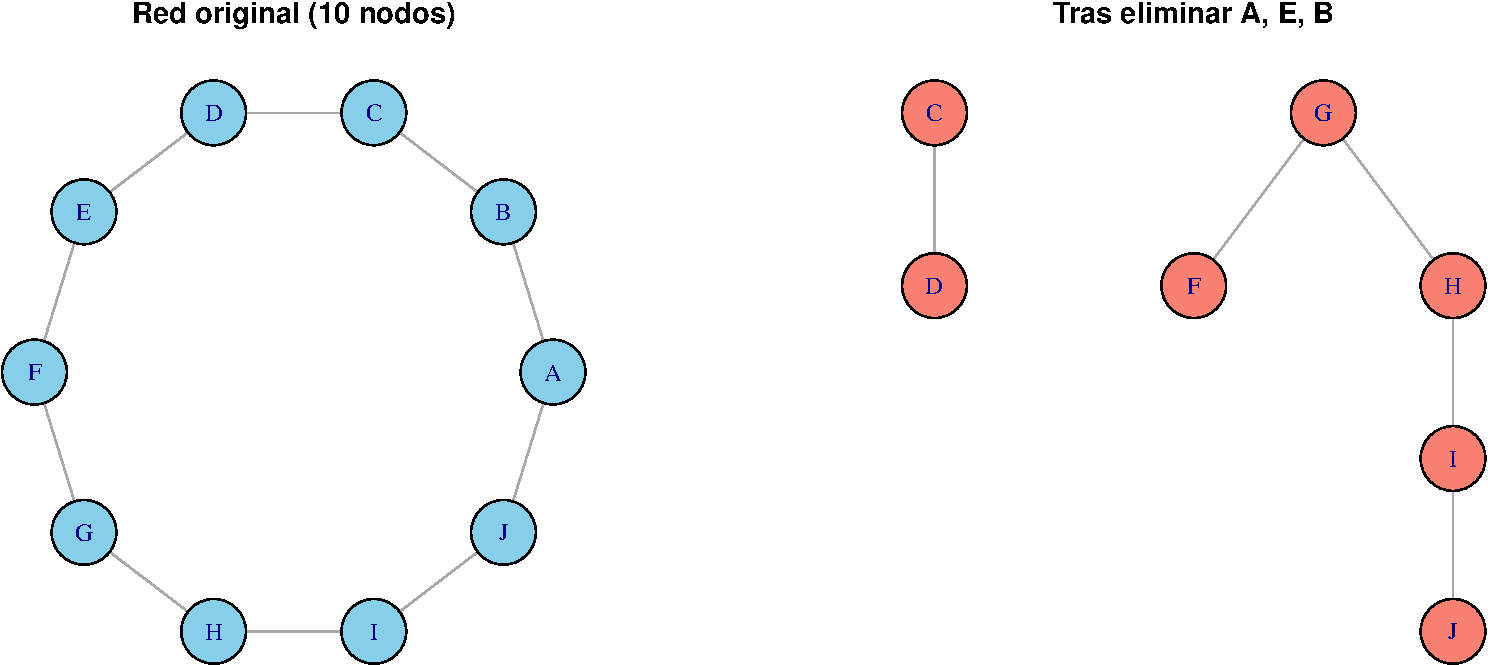
\includegraphics[keepaspectratio]{05-robustez_files/figure-pdf/fig-delete-vertices-demo-1.pdf}}

}

\caption{\label{fig-delete-vertices-demo}Eliminación de nodos en una red
anillo: antes (izq.) y después (der.)}

\end{figure}%

\begin{Shaded}
\begin{Highlighting}[]
\FunctionTok{cat}\NormalTok{(}\StringTok{"=== Red original ===}\SpecialCharTok{\textbackslash{}n}\StringTok{"}\NormalTok{)}
\end{Highlighting}
\end{Shaded}

\begin{verbatim}
=== Red original ===
\end{verbatim}

\begin{Shaded}
\begin{Highlighting}[]
\FunctionTok{cat}\NormalTok{(}\StringTok{"Nodos:"}\NormalTok{, }\FunctionTok{vcount}\NormalTok{(g), }\StringTok{" | Aristas:"}\NormalTok{, }\FunctionTok{ecount}\NormalTok{(g), }\StringTok{"}\SpecialCharTok{\textbackslash{}n}\StringTok{"}\NormalTok{)}
\end{Highlighting}
\end{Shaded}

\begin{verbatim}
Nodos: 10  | Aristas: 10 
\end{verbatim}

\begin{Shaded}
\begin{Highlighting}[]
\FunctionTok{cat}\NormalTok{(}\StringTok{"Componentes:"}\NormalTok{, }\FunctionTok{components}\NormalTok{(g)}\SpecialCharTok{$}\NormalTok{no, }\StringTok{"}\SpecialCharTok{\textbackslash{}n}\StringTok{"}\NormalTok{)}
\end{Highlighting}
\end{Shaded}

\begin{verbatim}
Componentes: 1 
\end{verbatim}

\begin{Shaded}
\begin{Highlighting}[]
\FunctionTok{cat}\NormalTok{(}\StringTok{"Distancia media:"}\NormalTok{, }\FunctionTok{round}\NormalTok{(}\FunctionTok{mean\_distance}\NormalTok{(g), }\DecValTok{3}\NormalTok{), }\StringTok{"}\SpecialCharTok{\textbackslash{}n\textbackslash{}n}\StringTok{"}\NormalTok{)}
\end{Highlighting}
\end{Shaded}

\begin{verbatim}
Distancia media: 2.778 
\end{verbatim}

\begin{Shaded}
\begin{Highlighting}[]
\FunctionTok{cat}\NormalTok{(}\StringTok{"=== Tras eliminar A, E, B ===}\SpecialCharTok{\textbackslash{}n}\StringTok{"}\NormalTok{)}
\end{Highlighting}
\end{Shaded}

\begin{verbatim}
=== Tras eliminar A, E, B ===
\end{verbatim}

\begin{Shaded}
\begin{Highlighting}[]
\FunctionTok{cat}\NormalTok{(}\StringTok{"Nodos:"}\NormalTok{, }\FunctionTok{vcount}\NormalTok{(g2), }\StringTok{" | Aristas:"}\NormalTok{, }\FunctionTok{ecount}\NormalTok{(g2), }\StringTok{"}\SpecialCharTok{\textbackslash{}n}\StringTok{"}\NormalTok{)}
\end{Highlighting}
\end{Shaded}

\begin{verbatim}
Nodos: 7  | Aristas: 5 
\end{verbatim}

\begin{Shaded}
\begin{Highlighting}[]
\FunctionTok{cat}\NormalTok{(}\StringTok{"Componentes:"}\NormalTok{, }\FunctionTok{components}\NormalTok{(g2)}\SpecialCharTok{$}\NormalTok{no, }\StringTok{"}\SpecialCharTok{\textbackslash{}n}\StringTok{"}\NormalTok{)}
\end{Highlighting}
\end{Shaded}

\begin{verbatim}
Componentes: 2 
\end{verbatim}

\begin{Shaded}
\begin{Highlighting}[]
\FunctionTok{cat}\NormalTok{(}\StringTok{"Distancia media:"}\NormalTok{, }\FunctionTok{round}\NormalTok{(}\FunctionTok{mean\_distance}\NormalTok{(g2), }\DecValTok{3}\NormalTok{), }\StringTok{"}\SpecialCharTok{\textbackslash{}n}\StringTok{"}\NormalTok{)}
\end{Highlighting}
\end{Shaded}

\begin{verbatim}
Distancia media: 1.909 
\end{verbatim}

\begin{tcolorbox}[enhanced jigsaw, colback=white, toprule=.15mm, title=\textcolor{quarto-callout-warning-color}{\faExclamationTriangle}\hspace{0.5em}{⚠️ Error frecuente}, titlerule=0mm, colframe=quarto-callout-warning-color-frame, breakable, opacitybacktitle=0.6, toptitle=1mm, left=2mm, bottomrule=.15mm, bottomtitle=1mm, arc=.35mm, rightrule=.15mm, leftrule=.75mm, opacityback=0, coltitle=black, colbacktitle=quarto-callout-warning-color!10!white]

Después de \texttt{delete\_vertices()}, los \textbf{índices de los nodos
cambian}. Si eliminas el nodo 1, el que antes era nodo 2 ahora es nodo
1. Por eso es preferible trabajar con \textbf{nombres}
(\texttt{V(g)\$name}) en vez de índices numéricos cuando eliminas nodos
iterativamente.

\end{tcolorbox}

\section{El componente gigante}\label{el-componente-gigante}

Cuando eliminamos nodos, la red puede fragmentarse en componentes
desconectados. El \textbf{componente gigante} es el componente conectado
más grande. Su tamaño relativo (como fracción del total de nodos
restantes) es la métrica principal de robustez:

\[
S = \frac{|C_{\max}|}{n_{\text{restantes}}}
\]

Si \(S \approx 1\), la red sigue funcionando. Si \(S \ll 1\), la red se
fragmentó.

\begin{Shaded}
\begin{Highlighting}[]
\CommentTok{\# Función auxiliar: tamaño relativo del componente gigante}
\NormalTok{tamano\_gigante }\OtherTok{\textless{}{-}} \ControlFlowTok{function}\NormalTok{(g) \{}
\NormalTok{  comp }\OtherTok{\textless{}{-}} \FunctionTok{components}\NormalTok{(g)}
  \FunctionTok{max}\NormalTok{(comp}\SpecialCharTok{$}\NormalTok{csize) }\SpecialCharTok{/} \FunctionTok{vcount}\NormalTok{(g)}
\NormalTok{\}}

\FunctionTok{cat}\NormalTok{(}\StringTok{"Componente gigante (original):"}\NormalTok{, }\FunctionTok{tamano\_gigante}\NormalTok{(g), }\StringTok{"}\SpecialCharTok{\textbackslash{}n}\StringTok{"}\NormalTok{)}
\end{Highlighting}
\end{Shaded}

\begin{verbatim}
Componente gigante (original): 1 
\end{verbatim}

\begin{Shaded}
\begin{Highlighting}[]
\FunctionTok{cat}\NormalTok{(}\StringTok{"Componente gigante (tras eliminar 3 nodos):"}\NormalTok{, }
    \FunctionTok{round}\NormalTok{(}\FunctionTok{tamano\_gigante}\NormalTok{(g2), }\DecValTok{3}\NormalTok{), }\StringTok{"}\SpecialCharTok{\textbackslash{}n}\StringTok{"}\NormalTok{)}
\end{Highlighting}
\end{Shaded}

\begin{verbatim}
Componente gigante (tras eliminar 3 nodos): 0.714 
\end{verbatim}

\section{Simulación de fallos
aleatorios}\label{simulaciuxf3n-de-fallos-aleatorios}

Vamos a construir una función que elimine nodos al azar de forma
iterativa y registre las métricas en cada paso.

\begin{Shaded}
\begin{Highlighting}[]
\NormalTok{simular\_fallos }\OtherTok{\textless{}{-}} \ControlFlowTok{function}\NormalTok{(g, }\AttributeTok{fraccion\_eliminar =} \FloatTok{0.5}\NormalTok{, }\AttributeTok{semilla =} \DecValTok{42}\NormalTok{) \{}
  \FunctionTok{set.seed}\NormalTok{(semilla)}
\NormalTok{  n\_original }\OtherTok{\textless{}{-}} \FunctionTok{vcount}\NormalTok{(g)}
\NormalTok{  n\_eliminar }\OtherTok{\textless{}{-}} \FunctionTok{floor}\NormalTok{(n\_original }\SpecialCharTok{*}\NormalTok{ fraccion\_eliminar)}
  
  \CommentTok{\# Seleccionar nodos a eliminar en orden aleatorio}
\NormalTok{  orden\_eliminacion }\OtherTok{\textless{}{-}} \FunctionTok{sample}\NormalTok{(}\FunctionTok{V}\NormalTok{(g)}\SpecialCharTok{$}\NormalTok{name, n\_eliminar)}
  
  \CommentTok{\# Registrar métricas en cada paso}
\NormalTok{  resultados }\OtherTok{\textless{}{-}} \FunctionTok{data.frame}\NormalTok{(}
    \AttributeTok{eliminados =} \DecValTok{0}\SpecialCharTok{:}\NormalTok{n\_eliminar,}
    \AttributeTok{fraccion\_eliminada =}\NormalTok{ (}\DecValTok{0}\SpecialCharTok{:}\NormalTok{n\_eliminar) }\SpecialCharTok{/}\NormalTok{ n\_original,}
    \AttributeTok{comp\_gigante =} \FunctionTok{numeric}\NormalTok{(n\_eliminar }\SpecialCharTok{+} \DecValTok{1}\NormalTok{),}
    \AttributeTok{dist\_media =} \FunctionTok{numeric}\NormalTok{(n\_eliminar }\SpecialCharTok{+} \DecValTok{1}\NormalTok{),}
    \AttributeTok{diametro =} \FunctionTok{numeric}\NormalTok{(n\_eliminar }\SpecialCharTok{+} \DecValTok{1}\NormalTok{)}
\NormalTok{  )}
  
\NormalTok{  g\_temp }\OtherTok{\textless{}{-}}\NormalTok{ g}
  
  \ControlFlowTok{for}\NormalTok{ (i }\ControlFlowTok{in} \DecValTok{0}\SpecialCharTok{:}\NormalTok{n\_eliminar) \{}
    \ControlFlowTok{if}\NormalTok{ (i }\SpecialCharTok{\textgreater{}} \DecValTok{0}\NormalTok{) \{}
\NormalTok{      g\_temp }\OtherTok{\textless{}{-}} \FunctionTok{delete\_vertices}\NormalTok{(g\_temp, orden\_eliminacion[i])}
\NormalTok{    \}}
    
\NormalTok{    resultados}\SpecialCharTok{$}\NormalTok{comp\_gigante[i }\SpecialCharTok{+} \DecValTok{1}\NormalTok{] }\OtherTok{\textless{}{-}} \FunctionTok{tamano\_gigante}\NormalTok{(g\_temp)}
    
    \CommentTok{\# Calcular distancia media solo en el componente gigante}
\NormalTok{    comp }\OtherTok{\textless{}{-}} \FunctionTok{components}\NormalTok{(g\_temp)}
\NormalTok{    giant\_id }\OtherTok{\textless{}{-}} \FunctionTok{which.max}\NormalTok{(comp}\SpecialCharTok{$}\NormalTok{csize)}
\NormalTok{    giant\_nodes }\OtherTok{\textless{}{-}} \FunctionTok{which}\NormalTok{(comp}\SpecialCharTok{$}\NormalTok{membership }\SpecialCharTok{==}\NormalTok{ giant\_id)}
    \ControlFlowTok{if}\NormalTok{ (}\FunctionTok{length}\NormalTok{(giant\_nodes) }\SpecialCharTok{\textgreater{}} \DecValTok{1}\NormalTok{) \{}
\NormalTok{      g\_giant }\OtherTok{\textless{}{-}} \FunctionTok{induced\_subgraph}\NormalTok{(g\_temp, giant\_nodes)}
\NormalTok{      resultados}\SpecialCharTok{$}\NormalTok{dist\_media[i }\SpecialCharTok{+} \DecValTok{1}\NormalTok{] }\OtherTok{\textless{}{-}} \FunctionTok{mean\_distance}\NormalTok{(g\_giant)}
\NormalTok{      resultados}\SpecialCharTok{$}\NormalTok{diametro[i }\SpecialCharTok{+} \DecValTok{1}\NormalTok{] }\OtherTok{\textless{}{-}} \FunctionTok{diameter}\NormalTok{(g\_giant)}
\NormalTok{    \} }\ControlFlowTok{else}\NormalTok{ \{}
\NormalTok{      resultados}\SpecialCharTok{$}\NormalTok{dist\_media[i }\SpecialCharTok{+} \DecValTok{1}\NormalTok{] }\OtherTok{\textless{}{-}} \DecValTok{0}
\NormalTok{      resultados}\SpecialCharTok{$}\NormalTok{diametro[i }\SpecialCharTok{+} \DecValTok{1}\NormalTok{] }\OtherTok{\textless{}{-}} \DecValTok{0}
\NormalTok{    \}}
\NormalTok{  \}}
  
\NormalTok{  resultados}
\NormalTok{\}}
\end{Highlighting}
\end{Shaded}

En un ataque dirigido, eliminamos los nodos \textbf{más conectados
primero}. Recalculamos el grado después de cada eliminación, porque el
nodo más conectado puede cambiar.

\begin{Shaded}
\begin{Highlighting}[]
\NormalTok{simular\_ataques }\OtherTok{\textless{}{-}} \ControlFlowTok{function}\NormalTok{(g, }\AttributeTok{fraccion\_eliminar =} \FloatTok{0.5}\NormalTok{, }\AttributeTok{semilla =} \DecValTok{42}\NormalTok{) \{}
  \FunctionTok{set.seed}\NormalTok{(semilla)}
\NormalTok{  n\_original }\OtherTok{\textless{}{-}} \FunctionTok{vcount}\NormalTok{(g)}
\NormalTok{  n\_eliminar }\OtherTok{\textless{}{-}} \FunctionTok{floor}\NormalTok{(n\_original }\SpecialCharTok{*}\NormalTok{ fraccion\_eliminar)}
  
\NormalTok{  resultados }\OtherTok{\textless{}{-}} \FunctionTok{data.frame}\NormalTok{(}
    \AttributeTok{eliminados =} \DecValTok{0}\SpecialCharTok{:}\NormalTok{n\_eliminar,}
    \AttributeTok{fraccion\_eliminada =}\NormalTok{ (}\DecValTok{0}\SpecialCharTok{:}\NormalTok{n\_eliminar) }\SpecialCharTok{/}\NormalTok{ n\_original,}
    \AttributeTok{comp\_gigante =} \FunctionTok{numeric}\NormalTok{(n\_eliminar }\SpecialCharTok{+} \DecValTok{1}\NormalTok{),}
    \AttributeTok{dist\_media =} \FunctionTok{numeric}\NormalTok{(n\_eliminar }\SpecialCharTok{+} \DecValTok{1}\NormalTok{),}
    \AttributeTok{diametro =} \FunctionTok{numeric}\NormalTok{(n\_eliminar }\SpecialCharTok{+} \DecValTok{1}\NormalTok{)}
\NormalTok{  )}
  
\NormalTok{  g\_temp }\OtherTok{\textless{}{-}}\NormalTok{ g}
  
  \ControlFlowTok{for}\NormalTok{ (i }\ControlFlowTok{in} \DecValTok{0}\SpecialCharTok{:}\NormalTok{n\_eliminar) \{}
    \ControlFlowTok{if}\NormalTok{ (i }\SpecialCharTok{\textgreater{}} \DecValTok{0}\NormalTok{) \{}
      \CommentTok{\# Identificar el nodo con mayor grado (recalculado)}
\NormalTok{      deg }\OtherTok{\textless{}{-}} \FunctionTok{degree}\NormalTok{(g\_temp)}
\NormalTok{      hub }\OtherTok{\textless{}{-}} \FunctionTok{V}\NormalTok{(g\_temp)}\SpecialCharTok{$}\NormalTok{name[}\FunctionTok{which.max}\NormalTok{(deg)]}
\NormalTok{      g\_temp }\OtherTok{\textless{}{-}} \FunctionTok{delete\_vertices}\NormalTok{(g\_temp, hub)}
\NormalTok{    \}}
    
\NormalTok{    resultados}\SpecialCharTok{$}\NormalTok{comp\_gigante[i }\SpecialCharTok{+} \DecValTok{1}\NormalTok{] }\OtherTok{\textless{}{-}} \FunctionTok{tamano\_gigante}\NormalTok{(g\_temp)}
    
    \CommentTok{\# Calcular distancia media solo en el componente gigante}
\NormalTok{    comp }\OtherTok{\textless{}{-}} \FunctionTok{components}\NormalTok{(g\_temp)}
\NormalTok{    giant\_id }\OtherTok{\textless{}{-}} \FunctionTok{which.max}\NormalTok{(comp}\SpecialCharTok{$}\NormalTok{csize)}
\NormalTok{    giant\_nodes }\OtherTok{\textless{}{-}} \FunctionTok{which}\NormalTok{(comp}\SpecialCharTok{$}\NormalTok{membership }\SpecialCharTok{==}\NormalTok{ giant\_id)}
    \ControlFlowTok{if}\NormalTok{ (}\FunctionTok{length}\NormalTok{(giant\_nodes) }\SpecialCharTok{\textgreater{}} \DecValTok{1}\NormalTok{) \{}
\NormalTok{      g\_giant }\OtherTok{\textless{}{-}} \FunctionTok{induced\_subgraph}\NormalTok{(g\_temp, giant\_nodes)}
\NormalTok{      resultados}\SpecialCharTok{$}\NormalTok{dist\_media[i }\SpecialCharTok{+} \DecValTok{1}\NormalTok{] }\OtherTok{\textless{}{-}} \FunctionTok{mean\_distance}\NormalTok{(g\_giant)}
\NormalTok{      resultados}\SpecialCharTok{$}\NormalTok{diametro[i }\SpecialCharTok{+} \DecValTok{1}\NormalTok{] }\OtherTok{\textless{}{-}} \FunctionTok{diameter}\NormalTok{(g\_giant)}
\NormalTok{    \} }\ControlFlowTok{else}\NormalTok{ \{}
\NormalTok{      resultados}\SpecialCharTok{$}\NormalTok{dist\_media[i }\SpecialCharTok{+} \DecValTok{1}\NormalTok{] }\OtherTok{\textless{}{-}} \DecValTok{0}
\NormalTok{      resultados}\SpecialCharTok{$}\NormalTok{diametro[i }\SpecialCharTok{+} \DecValTok{1}\NormalTok{] }\OtherTok{\textless{}{-}} \DecValTok{0}
\NormalTok{    \}}
\NormalTok{  \}}
  
\NormalTok{  resultados}
\NormalTok{\}}
\end{Highlighting}
\end{Shaded}

\begin{tcolorbox}[enhanced jigsaw, colback=white, toprule=.15mm, title=\textcolor{quarto-callout-important-color}{\faExclamation}\hspace{0.5em}{🔑 Recuerda}, titlerule=0mm, colframe=quarto-callout-important-color-frame, breakable, opacitybacktitle=0.6, toptitle=1mm, left=2mm, bottomrule=.15mm, bottomtitle=1mm, arc=.35mm, rightrule=.15mm, leftrule=.75mm, opacityback=0, coltitle=black, colbacktitle=quarto-callout-important-color!10!white]

En la simulación de ataques, es crucial \textbf{recalcular el grado} en
cada paso. Después de eliminar un \emph{hub}, otro nodo puede
convertirse en el nuevo más conectado. Esto hace que la simulación sea
más lenta pero realista.

\end{tcolorbox}

\section{Experimento: ER vs.~BA bajo fallos y
ataques}\label{experimento-er-vs.-ba-bajo-fallos-y-ataques}

Ahora viene el experimento central del capítulo. Generaremos una red
Erdős--Rényi y una Barabási--Albert de tamaño similar, y las someteremos
a ambos tipos de perturbación.

\begin{Shaded}
\begin{Highlighting}[]
\FunctionTok{set.seed}\NormalTok{(}\DecValTok{123}\NormalTok{)}

\NormalTok{n }\OtherTok{\textless{}{-}} \DecValTok{500}

\CommentTok{\# Red ER con \textasciitilde{}1000 aristas}
\NormalTok{g\_er }\OtherTok{\textless{}{-}} \FunctionTok{sample\_gnp}\NormalTok{(n, }\AttributeTok{p =} \DecValTok{2} \SpecialCharTok{/}\NormalTok{ (n }\SpecialCharTok{{-}} \DecValTok{1}\NormalTok{) }\SpecialCharTok{*} \DecValTok{2}\NormalTok{)}
\FunctionTok{V}\NormalTok{(g\_er)}\SpecialCharTok{$}\NormalTok{name }\OtherTok{\textless{}{-}} \FunctionTok{paste0}\NormalTok{(}\StringTok{"ER\_"}\NormalTok{, }\DecValTok{1}\SpecialCharTok{:}\FunctionTok{vcount}\NormalTok{(g\_er))}

\CommentTok{\# Red BA con parámetro m = 2 (\textasciitilde{}1000 aristas)}
\NormalTok{g\_ba }\OtherTok{\textless{}{-}} \FunctionTok{sample\_pa}\NormalTok{(n, }\AttributeTok{m =} \DecValTok{2}\NormalTok{, }\AttributeTok{directed =} \ConstantTok{FALSE}\NormalTok{)}
\FunctionTok{V}\NormalTok{(g\_ba)}\SpecialCharTok{$}\NormalTok{name }\OtherTok{\textless{}{-}} \FunctionTok{paste0}\NormalTok{(}\StringTok{"BA\_"}\NormalTok{, }\DecValTok{1}\SpecialCharTok{:}\FunctionTok{vcount}\NormalTok{(g\_ba))}

\FunctionTok{cat}\NormalTok{(}\StringTok{"=== Red Erdős–Rényi ===}\SpecialCharTok{\textbackslash{}n}\StringTok{"}\NormalTok{)}
\end{Highlighting}
\end{Shaded}

\begin{verbatim}
=== Red Erdős–Rényi ===
\end{verbatim}

\begin{Shaded}
\begin{Highlighting}[]
\FunctionTok{cat}\NormalTok{(}\StringTok{"Nodos:"}\NormalTok{, }\FunctionTok{vcount}\NormalTok{(g\_er), }\StringTok{" | Aristas:"}\NormalTok{, }\FunctionTok{ecount}\NormalTok{(g\_er), }\StringTok{"}\SpecialCharTok{\textbackslash{}n}\StringTok{"}\NormalTok{)}
\end{Highlighting}
\end{Shaded}

\begin{verbatim}
Nodos: 500  | Aristas: 965 
\end{verbatim}

\begin{Shaded}
\begin{Highlighting}[]
\FunctionTok{cat}\NormalTok{(}\StringTok{"Grado medio:"}\NormalTok{, }\FunctionTok{round}\NormalTok{(}\FunctionTok{mean}\NormalTok{(}\FunctionTok{degree}\NormalTok{(g\_er)), }\DecValTok{2}\NormalTok{), }\StringTok{"}\SpecialCharTok{\textbackslash{}n}\StringTok{"}\NormalTok{)}
\end{Highlighting}
\end{Shaded}

\begin{verbatim}
Grado medio: 3.86 
\end{verbatim}

\begin{Shaded}
\begin{Highlighting}[]
\FunctionTok{cat}\NormalTok{(}\StringTok{"Grado máximo:"}\NormalTok{, }\FunctionTok{max}\NormalTok{(}\FunctionTok{degree}\NormalTok{(g\_er)), }\StringTok{"}\SpecialCharTok{\textbackslash{}n\textbackslash{}n}\StringTok{"}\NormalTok{)}
\end{Highlighting}
\end{Shaded}

\begin{verbatim}
Grado máximo: 10 
\end{verbatim}

\begin{Shaded}
\begin{Highlighting}[]
\FunctionTok{cat}\NormalTok{(}\StringTok{"=== Red Barabási–Albert ===}\SpecialCharTok{\textbackslash{}n}\StringTok{"}\NormalTok{)}
\end{Highlighting}
\end{Shaded}

\begin{verbatim}
=== Red Barabási–Albert ===
\end{verbatim}

\begin{Shaded}
\begin{Highlighting}[]
\FunctionTok{cat}\NormalTok{(}\StringTok{"Nodos:"}\NormalTok{, }\FunctionTok{vcount}\NormalTok{(g\_ba), }\StringTok{" | Aristas:"}\NormalTok{, }\FunctionTok{ecount}\NormalTok{(g\_ba), }\StringTok{"}\SpecialCharTok{\textbackslash{}n}\StringTok{"}\NormalTok{)}
\end{Highlighting}
\end{Shaded}

\begin{verbatim}
Nodos: 500  | Aristas: 997 
\end{verbatim}

\begin{Shaded}
\begin{Highlighting}[]
\FunctionTok{cat}\NormalTok{(}\StringTok{"Grado medio:"}\NormalTok{, }\FunctionTok{round}\NormalTok{(}\FunctionTok{mean}\NormalTok{(}\FunctionTok{degree}\NormalTok{(g\_ba)), }\DecValTok{2}\NormalTok{), }\StringTok{"}\SpecialCharTok{\textbackslash{}n}\StringTok{"}\NormalTok{)}
\end{Highlighting}
\end{Shaded}

\begin{verbatim}
Grado medio: 3.99 
\end{verbatim}

\begin{Shaded}
\begin{Highlighting}[]
\FunctionTok{cat}\NormalTok{(}\StringTok{"Grado máximo:"}\NormalTok{, }\FunctionTok{max}\NormalTok{(}\FunctionTok{degree}\NormalTok{(g\_ba)), }\StringTok{"}\SpecialCharTok{\textbackslash{}n}\StringTok{"}\NormalTok{)}
\end{Highlighting}
\end{Shaded}

\begin{verbatim}
Grado máximo: 54 
\end{verbatim}

\begin{Shaded}
\begin{Highlighting}[]
\CommentTok{\# Simular los 4 escenarios}
\NormalTok{fallo\_er  }\OtherTok{\textless{}{-}} \FunctionTok{simular\_fallos}\NormalTok{(g\_er, }\AttributeTok{fraccion\_eliminar =} \FloatTok{0.4}\NormalTok{)}
\NormalTok{fallo\_ba  }\OtherTok{\textless{}{-}} \FunctionTok{simular\_fallos}\NormalTok{(g\_ba, }\AttributeTok{fraccion\_eliminar =} \FloatTok{0.4}\NormalTok{)}
\NormalTok{ataque\_er }\OtherTok{\textless{}{-}} \FunctionTok{simular\_ataques}\NormalTok{(g\_er, }\AttributeTok{fraccion\_eliminar =} \FloatTok{0.4}\NormalTok{)}
\NormalTok{ataque\_ba }\OtherTok{\textless{}{-}} \FunctionTok{simular\_ataques}\NormalTok{(g\_ba, }\AttributeTok{fraccion\_eliminar =} \FloatTok{0.4}\NormalTok{)}
\end{Highlighting}
\end{Shaded}

\subsection{Resultado 1: Componente
gigante}\label{resultado-1-componente-gigante}

\begin{Shaded}
\begin{Highlighting}[]
\FunctionTok{par}\NormalTok{(}\AttributeTok{mfrow =} \FunctionTok{c}\NormalTok{(}\DecValTok{1}\NormalTok{, }\DecValTok{2}\NormalTok{), }\AttributeTok{mar =} \FunctionTok{c}\NormalTok{(}\DecValTok{4}\NormalTok{, }\DecValTok{4}\NormalTok{, }\DecValTok{3}\NormalTok{, }\DecValTok{1}\NormalTok{))}

\CommentTok{\# Fallos aleatorios}
\FunctionTok{plot}\NormalTok{(fallo\_er}\SpecialCharTok{$}\NormalTok{fraccion\_eliminada, fallo\_er}\SpecialCharTok{$}\NormalTok{comp\_gigante,}
     \AttributeTok{type =} \StringTok{"l"}\NormalTok{, }\AttributeTok{lwd =} \FloatTok{2.5}\NormalTok{, }\AttributeTok{col =} \StringTok{"skyblue"}\NormalTok{,}
     \AttributeTok{xlab =} \StringTok{"Fracción de nodos eliminados"}\NormalTok{,}
     \AttributeTok{ylab =} \StringTok{"Tamaño relativo del componente gigante"}\NormalTok{,}
     \AttributeTok{main =} \StringTok{"Fallos aleatorios"}\NormalTok{,}
     \AttributeTok{ylim =} \FunctionTok{c}\NormalTok{(}\DecValTok{0}\NormalTok{, }\DecValTok{1}\NormalTok{))}
\FunctionTok{lines}\NormalTok{(fallo\_ba}\SpecialCharTok{$}\NormalTok{fraccion\_eliminada, fallo\_ba}\SpecialCharTok{$}\NormalTok{comp\_gigante,}
      \AttributeTok{lwd =} \FloatTok{2.5}\NormalTok{, }\AttributeTok{col =} \StringTok{"tomato"}\NormalTok{)}
\FunctionTok{legend}\NormalTok{(}\StringTok{"topright"}\NormalTok{, }\AttributeTok{legend =} \FunctionTok{c}\NormalTok{(}\StringTok{"ER"}\NormalTok{, }\StringTok{"BA"}\NormalTok{),}
       \AttributeTok{col =} \FunctionTok{c}\NormalTok{(}\StringTok{"skyblue"}\NormalTok{, }\StringTok{"tomato"}\NormalTok{), }\AttributeTok{lwd =} \FloatTok{2.5}\NormalTok{, }\AttributeTok{bty =} \StringTok{"n"}\NormalTok{)}

\CommentTok{\# Ataques dirigidos}
\FunctionTok{plot}\NormalTok{(ataque\_er}\SpecialCharTok{$}\NormalTok{fraccion\_eliminada, ataque\_er}\SpecialCharTok{$}\NormalTok{comp\_gigante,}
     \AttributeTok{type =} \StringTok{"l"}\NormalTok{, }\AttributeTok{lwd =} \FloatTok{2.5}\NormalTok{, }\AttributeTok{col =} \StringTok{"skyblue"}\NormalTok{,}
     \AttributeTok{xlab =} \StringTok{"Fracción de nodos eliminados"}\NormalTok{,}
     \AttributeTok{ylab =} \StringTok{"Tamaño relativo del componente gigante"}\NormalTok{,}
     \AttributeTok{main =} \StringTok{"Ataques dirigidos (hubs primero)"}\NormalTok{,}
     \AttributeTok{ylim =} \FunctionTok{c}\NormalTok{(}\DecValTok{0}\NormalTok{, }\DecValTok{1}\NormalTok{))}
\FunctionTok{lines}\NormalTok{(ataque\_ba}\SpecialCharTok{$}\NormalTok{fraccion\_eliminada, ataque\_ba}\SpecialCharTok{$}\NormalTok{comp\_gigante,}
      \AttributeTok{lwd =} \FloatTok{2.5}\NormalTok{, }\AttributeTok{col =} \StringTok{"tomato"}\NormalTok{)}
\FunctionTok{legend}\NormalTok{(}\StringTok{"topright"}\NormalTok{, }\AttributeTok{legend =} \FunctionTok{c}\NormalTok{(}\StringTok{"ER"}\NormalTok{, }\StringTok{"BA"}\NormalTok{),}
       \AttributeTok{col =} \FunctionTok{c}\NormalTok{(}\StringTok{"skyblue"}\NormalTok{, }\StringTok{"tomato"}\NormalTok{), }\AttributeTok{lwd =} \FloatTok{2.5}\NormalTok{, }\AttributeTok{bty =} \StringTok{"n"}\NormalTok{)}
\end{Highlighting}
\end{Shaded}

\begin{figure}[H]

\centering{

\pandocbounded{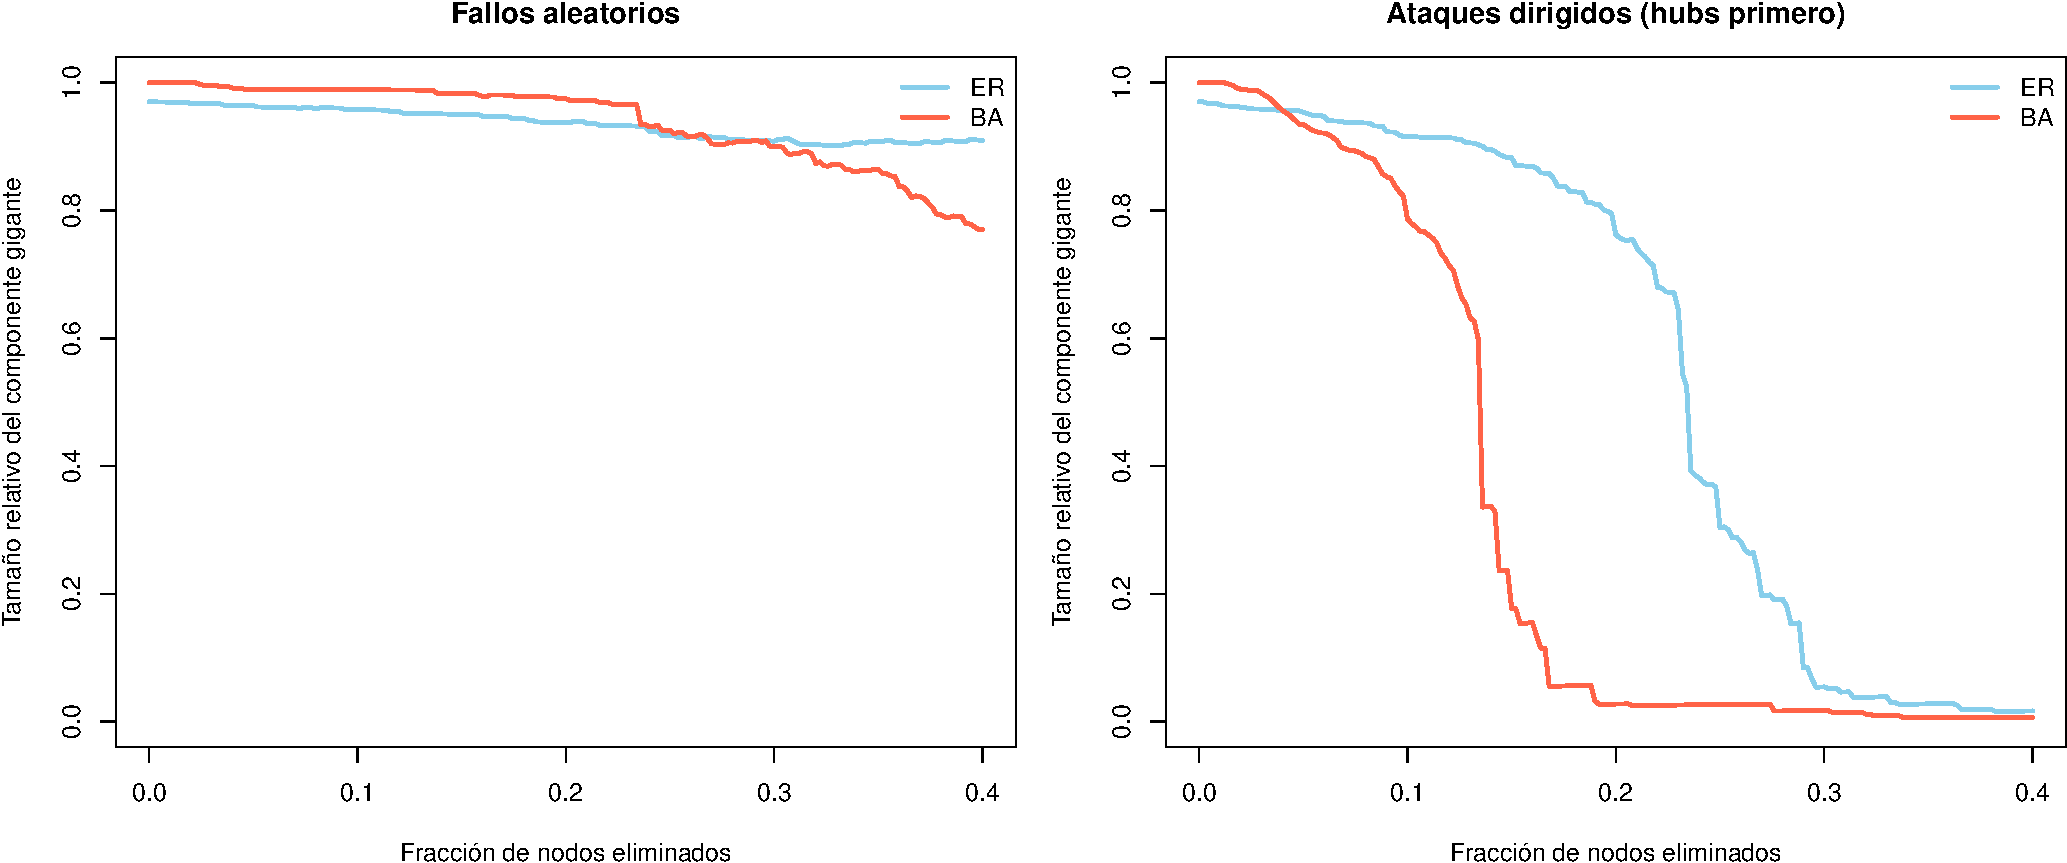
\includegraphics[keepaspectratio]{05-robustez_files/figure-pdf/fig-robustez-comp-gigante-1.pdf}}

}

\caption{\label{fig-robustez-comp-gigante}Tamaño del componente gigante
bajo fallos aleatorios (izq.) y ataques dirigidos (der.)}

\end{figure}%

\begin{tcolorbox}[enhanced jigsaw, colback=white, toprule=.15mm, title=\textcolor{quarto-callout-tip-color}{\faLightbulb}\hspace{0.5em}{💡 Concepto clave}, titlerule=0mm, colframe=quarto-callout-tip-color-frame, breakable, opacitybacktitle=0.6, toptitle=1mm, left=2mm, bottomrule=.15mm, bottomtitle=1mm, arc=.35mm, rightrule=.15mm, leftrule=.75mm, opacityback=0, coltitle=black, colbacktitle=quarto-callout-tip-color!10!white]

Este es el resultado más famoso de la robustez de redes (Albert et al.,
2000):

\begin{itemize}
\tightlist
\item
  \textbf{Ante fallos aleatorios}, la red BA es \textbf{más robusta} que
  la ER: como la mayoría de sus nodos tienen grado bajo, es improbable
  que un fallo aleatorio afecte un \emph{hub}.
\item
  \textbf{Ante ataques dirigidos}, la red BA es \textbf{extremadamente
  vulnerable}: eliminar unos pocos \emph{hubs} destruye la conectividad
  global. La red ER, sin \emph{hubs}, resiste mejor.
\end{itemize}

Esta dualidad se conoce como la paradoja de la
\textbf{robustez-fragilidad} de las redes \emph{scale-free}.

\end{tcolorbox}

\subsection{Resultado 2: Distancia
media}\label{resultado-2-distancia-media}

\begin{Shaded}
\begin{Highlighting}[]
\FunctionTok{par}\NormalTok{(}\AttributeTok{mfrow =} \FunctionTok{c}\NormalTok{(}\DecValTok{1}\NormalTok{, }\DecValTok{2}\NormalTok{), }\AttributeTok{mar =} \FunctionTok{c}\NormalTok{(}\DecValTok{4}\NormalTok{, }\DecValTok{4}\NormalTok{, }\DecValTok{3}\NormalTok{, }\DecValTok{1}\NormalTok{))}

\CommentTok{\# Calcular ylim seguro para distancias}
\NormalTok{all\_dist }\OtherTok{\textless{}{-}} \FunctionTok{c}\NormalTok{(fallo\_er}\SpecialCharTok{$}\NormalTok{dist\_media, fallo\_ba}\SpecialCharTok{$}\NormalTok{dist\_media, }
\NormalTok{              ataque\_er}\SpecialCharTok{$}\NormalTok{dist\_media, ataque\_ba}\SpecialCharTok{$}\NormalTok{dist\_media)}
\NormalTok{ylim\_max }\OtherTok{\textless{}{-}} \FunctionTok{max}\NormalTok{(all\_dist, }\AttributeTok{na.rm =} \ConstantTok{TRUE}\NormalTok{)}
\ControlFlowTok{if}\NormalTok{ (}\SpecialCharTok{!}\FunctionTok{is.finite}\NormalTok{(ylim\_max) }\SpecialCharTok{||}\NormalTok{ ylim\_max }\SpecialCharTok{==} \DecValTok{0}\NormalTok{) ylim\_max }\OtherTok{\textless{}{-}} \DecValTok{10}
\NormalTok{ylim\_dist }\OtherTok{\textless{}{-}} \FunctionTok{c}\NormalTok{(}\DecValTok{0}\NormalTok{, ylim\_max }\SpecialCharTok{*} \FloatTok{1.1}\NormalTok{)}

\CommentTok{\# Fallos}
\FunctionTok{plot}\NormalTok{(fallo\_er}\SpecialCharTok{$}\NormalTok{fraccion\_eliminada, fallo\_er}\SpecialCharTok{$}\NormalTok{dist\_media,}
     \AttributeTok{type =} \StringTok{"l"}\NormalTok{, }\AttributeTok{lwd =} \FloatTok{2.5}\NormalTok{, }\AttributeTok{col =} \StringTok{"skyblue"}\NormalTok{,}
     \AttributeTok{xlab =} \StringTok{"Fracción de nodos eliminados"}\NormalTok{,}
     \AttributeTok{ylab =} \StringTok{"Distancia media"}\NormalTok{,}
     \AttributeTok{main =} \StringTok{"Distancia media — Fallos aleatorios"}\NormalTok{,}
     \AttributeTok{ylim =}\NormalTok{ ylim\_dist)}
\FunctionTok{lines}\NormalTok{(fallo\_ba}\SpecialCharTok{$}\NormalTok{fraccion\_eliminada, fallo\_ba}\SpecialCharTok{$}\NormalTok{dist\_media,}
      \AttributeTok{lwd =} \FloatTok{2.5}\NormalTok{, }\AttributeTok{col =} \StringTok{"tomato"}\NormalTok{)}
\FunctionTok{legend}\NormalTok{(}\StringTok{"topleft"}\NormalTok{, }\AttributeTok{legend =} \FunctionTok{c}\NormalTok{(}\StringTok{"ER"}\NormalTok{, }\StringTok{"BA"}\NormalTok{),}
       \AttributeTok{col =} \FunctionTok{c}\NormalTok{(}\StringTok{"skyblue"}\NormalTok{, }\StringTok{"tomato"}\NormalTok{), }\AttributeTok{lwd =} \FloatTok{2.5}\NormalTok{, }\AttributeTok{bty =} \StringTok{"n"}\NormalTok{)}

\CommentTok{\# Ataques}
\FunctionTok{plot}\NormalTok{(ataque\_er}\SpecialCharTok{$}\NormalTok{fraccion\_eliminada, ataque\_er}\SpecialCharTok{$}\NormalTok{dist\_media,}
     \AttributeTok{type =} \StringTok{"l"}\NormalTok{, }\AttributeTok{lwd =} \FloatTok{2.5}\NormalTok{, }\AttributeTok{col =} \StringTok{"skyblue"}\NormalTok{,}
     \AttributeTok{xlab =} \StringTok{"Fracción de nodos eliminados"}\NormalTok{,}
     \AttributeTok{ylab =} \StringTok{"Distancia media"}\NormalTok{,}
     \AttributeTok{main =} \StringTok{"Distancia media — Ataques dirigidos"}\NormalTok{,}
     \AttributeTok{ylim =}\NormalTok{ ylim\_dist)}
\FunctionTok{lines}\NormalTok{(ataque\_ba}\SpecialCharTok{$}\NormalTok{fraccion\_eliminada, ataque\_ba}\SpecialCharTok{$}\NormalTok{dist\_media,}
      \AttributeTok{lwd =} \FloatTok{2.5}\NormalTok{, }\AttributeTok{col =} \StringTok{"tomato"}\NormalTok{)}
\FunctionTok{legend}\NormalTok{(}\StringTok{"topleft"}\NormalTok{, }\AttributeTok{legend =} \FunctionTok{c}\NormalTok{(}\StringTok{"ER"}\NormalTok{, }\StringTok{"BA"}\NormalTok{),}
       \AttributeTok{col =} \FunctionTok{c}\NormalTok{(}\StringTok{"skyblue"}\NormalTok{, }\StringTok{"tomato"}\NormalTok{), }\AttributeTok{lwd =} \FloatTok{2.5}\NormalTok{, }\AttributeTok{bty =} \StringTok{"n"}\NormalTok{)}
\end{Highlighting}
\end{Shaded}

\begin{figure}[H]

\centering{

\pandocbounded{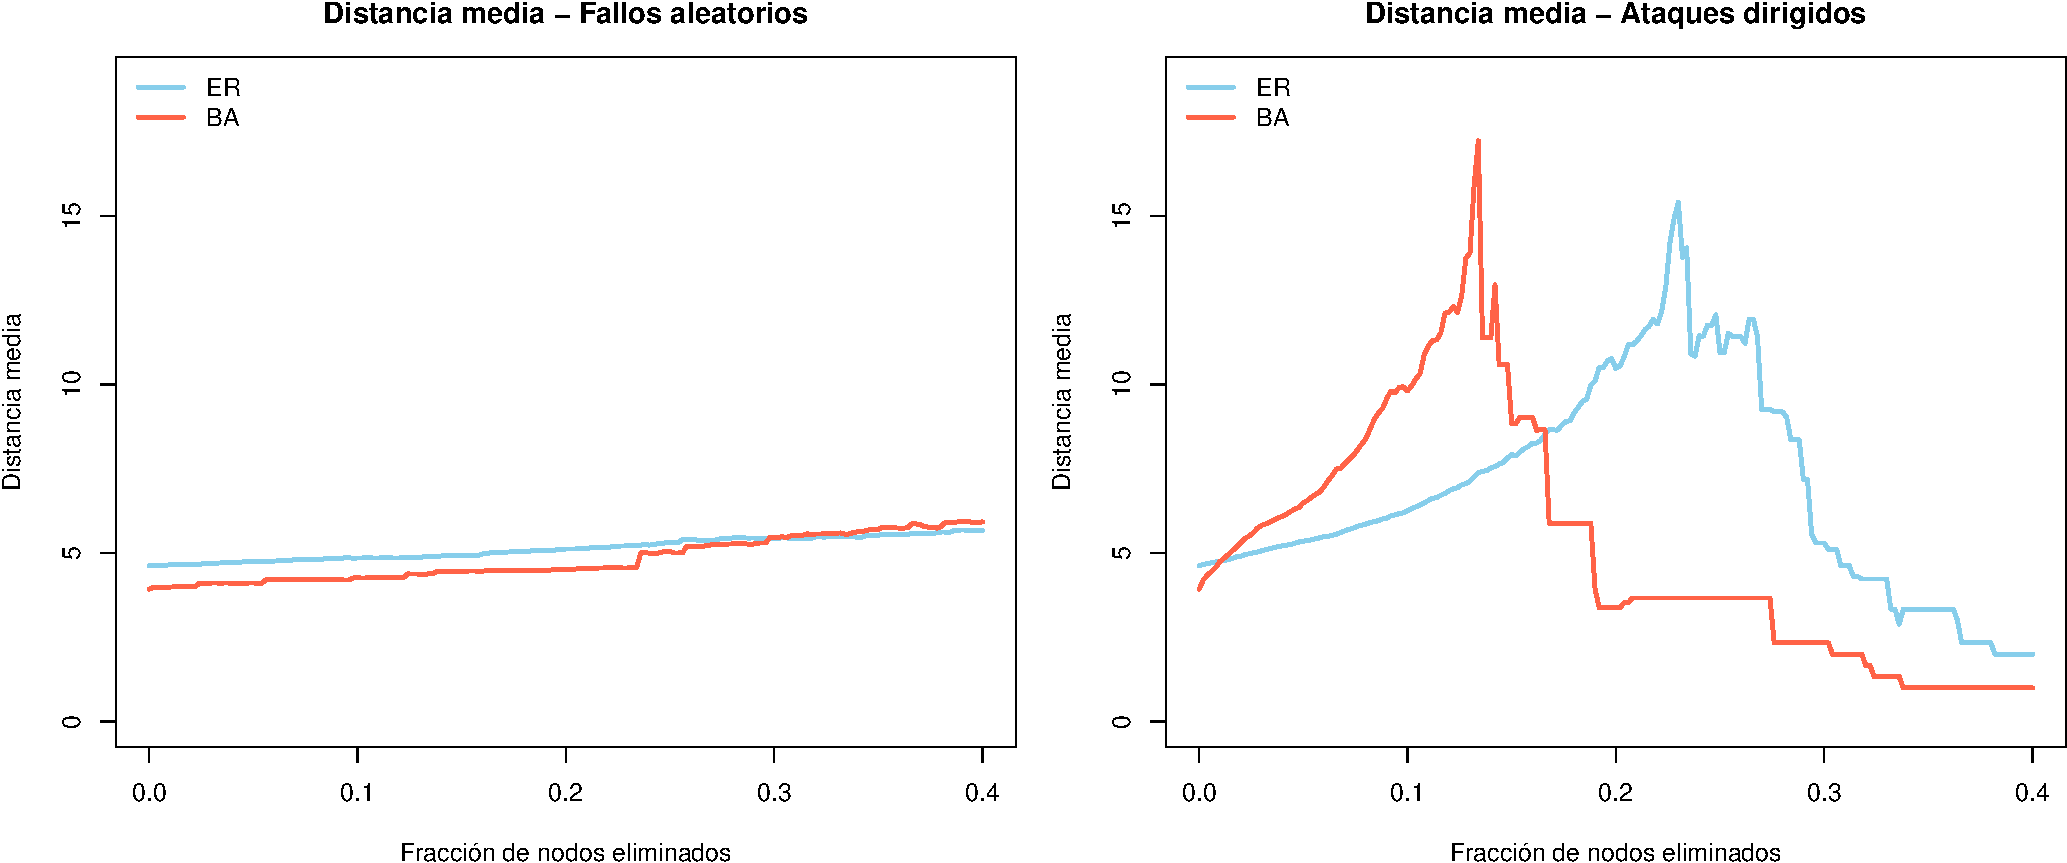
\includegraphics[keepaspectratio]{05-robustez_files/figure-pdf/fig-robustez-distancia-1.pdf}}

}

\caption{\label{fig-robustez-distancia}Evolución de la distancia media
bajo fallos (izq.) y ataques (der.)}

\end{figure}%

\subsection{Resultado 3: Diámetro}\label{resultado-3-diuxe1metro}

\begin{Shaded}
\begin{Highlighting}[]
\FunctionTok{par}\NormalTok{(}\AttributeTok{mfrow =} \FunctionTok{c}\NormalTok{(}\DecValTok{1}\NormalTok{, }\DecValTok{2}\NormalTok{), }\AttributeTok{mar =} \FunctionTok{c}\NormalTok{(}\DecValTok{4}\NormalTok{, }\DecValTok{4}\NormalTok{, }\DecValTok{3}\NormalTok{, }\DecValTok{1}\NormalTok{))}

\CommentTok{\# Calcular ylim seguro para diámetro}
\NormalTok{all\_diam }\OtherTok{\textless{}{-}} \FunctionTok{c}\NormalTok{(fallo\_er}\SpecialCharTok{$}\NormalTok{diametro, fallo\_ba}\SpecialCharTok{$}\NormalTok{diametro,}
\NormalTok{              ataque\_er}\SpecialCharTok{$}\NormalTok{diametro, ataque\_ba}\SpecialCharTok{$}\NormalTok{diametro)}
\NormalTok{ylim\_max\_d }\OtherTok{\textless{}{-}} \FunctionTok{max}\NormalTok{(all\_diam, }\AttributeTok{na.rm =} \ConstantTok{TRUE}\NormalTok{)}
\ControlFlowTok{if}\NormalTok{ (}\SpecialCharTok{!}\FunctionTok{is.finite}\NormalTok{(ylim\_max\_d) }\SpecialCharTok{||}\NormalTok{ ylim\_max\_d }\SpecialCharTok{==} \DecValTok{0}\NormalTok{) ylim\_max\_d }\OtherTok{\textless{}{-}} \DecValTok{10}
\NormalTok{ylim\_diam }\OtherTok{\textless{}{-}} \FunctionTok{c}\NormalTok{(}\DecValTok{0}\NormalTok{, ylim\_max\_d }\SpecialCharTok{*} \FloatTok{1.1}\NormalTok{)}

\CommentTok{\# Fallos}
\FunctionTok{plot}\NormalTok{(fallo\_er}\SpecialCharTok{$}\NormalTok{fraccion\_eliminada, fallo\_er}\SpecialCharTok{$}\NormalTok{diametro,}
     \AttributeTok{type =} \StringTok{"l"}\NormalTok{, }\AttributeTok{lwd =} \FloatTok{2.5}\NormalTok{, }\AttributeTok{col =} \StringTok{"skyblue"}\NormalTok{,}
     \AttributeTok{xlab =} \StringTok{"Fracción de nodos eliminados"}\NormalTok{,}
     \AttributeTok{ylab =} \StringTok{"Diámetro"}\NormalTok{,}
     \AttributeTok{main =} \StringTok{"Diámetro — Fallos aleatorios"}\NormalTok{,}
     \AttributeTok{ylim =}\NormalTok{ ylim\_diam)}
\FunctionTok{lines}\NormalTok{(fallo\_ba}\SpecialCharTok{$}\NormalTok{fraccion\_eliminada, fallo\_ba}\SpecialCharTok{$}\NormalTok{diametro,}
      \AttributeTok{lwd =} \FloatTok{2.5}\NormalTok{, }\AttributeTok{col =} \StringTok{"tomato"}\NormalTok{)}
\FunctionTok{legend}\NormalTok{(}\StringTok{"topleft"}\NormalTok{, }\AttributeTok{legend =} \FunctionTok{c}\NormalTok{(}\StringTok{"ER"}\NormalTok{, }\StringTok{"BA"}\NormalTok{),}
       \AttributeTok{col =} \FunctionTok{c}\NormalTok{(}\StringTok{"skyblue"}\NormalTok{, }\StringTok{"tomato"}\NormalTok{), }\AttributeTok{lwd =} \FloatTok{2.5}\NormalTok{, }\AttributeTok{bty =} \StringTok{"n"}\NormalTok{)}

\CommentTok{\# Ataques}
\FunctionTok{plot}\NormalTok{(ataque\_er}\SpecialCharTok{$}\NormalTok{fraccion\_eliminada, ataque\_er}\SpecialCharTok{$}\NormalTok{diametro,}
     \AttributeTok{type =} \StringTok{"l"}\NormalTok{, }\AttributeTok{lwd =} \FloatTok{2.5}\NormalTok{, }\AttributeTok{col =} \StringTok{"skyblue"}\NormalTok{,}
     \AttributeTok{xlab =} \StringTok{"Fracción de nodos eliminados"}\NormalTok{,}
     \AttributeTok{ylab =} \StringTok{"Diámetro"}\NormalTok{,}
     \AttributeTok{main =} \StringTok{"Diámetro — Ataques dirigidos"}\NormalTok{,}
     \AttributeTok{ylim =}\NormalTok{ ylim\_diam)}
\FunctionTok{lines}\NormalTok{(ataque\_ba}\SpecialCharTok{$}\NormalTok{fraccion\_eliminada, ataque\_ba}\SpecialCharTok{$}\NormalTok{diametro,}
      \AttributeTok{lwd =} \FloatTok{2.5}\NormalTok{, }\AttributeTok{col =} \StringTok{"tomato"}\NormalTok{)}
\FunctionTok{legend}\NormalTok{(}\StringTok{"topleft"}\NormalTok{, }\AttributeTok{legend =} \FunctionTok{c}\NormalTok{(}\StringTok{"ER"}\NormalTok{, }\StringTok{"BA"}\NormalTok{),}
       \AttributeTok{col =} \FunctionTok{c}\NormalTok{(}\StringTok{"skyblue"}\NormalTok{, }\StringTok{"tomato"}\NormalTok{), }\AttributeTok{lwd =} \FloatTok{2.5}\NormalTok{, }\AttributeTok{bty =} \StringTok{"n"}\NormalTok{)}
\end{Highlighting}
\end{Shaded}

\begin{figure}[H]

\centering{

\pandocbounded{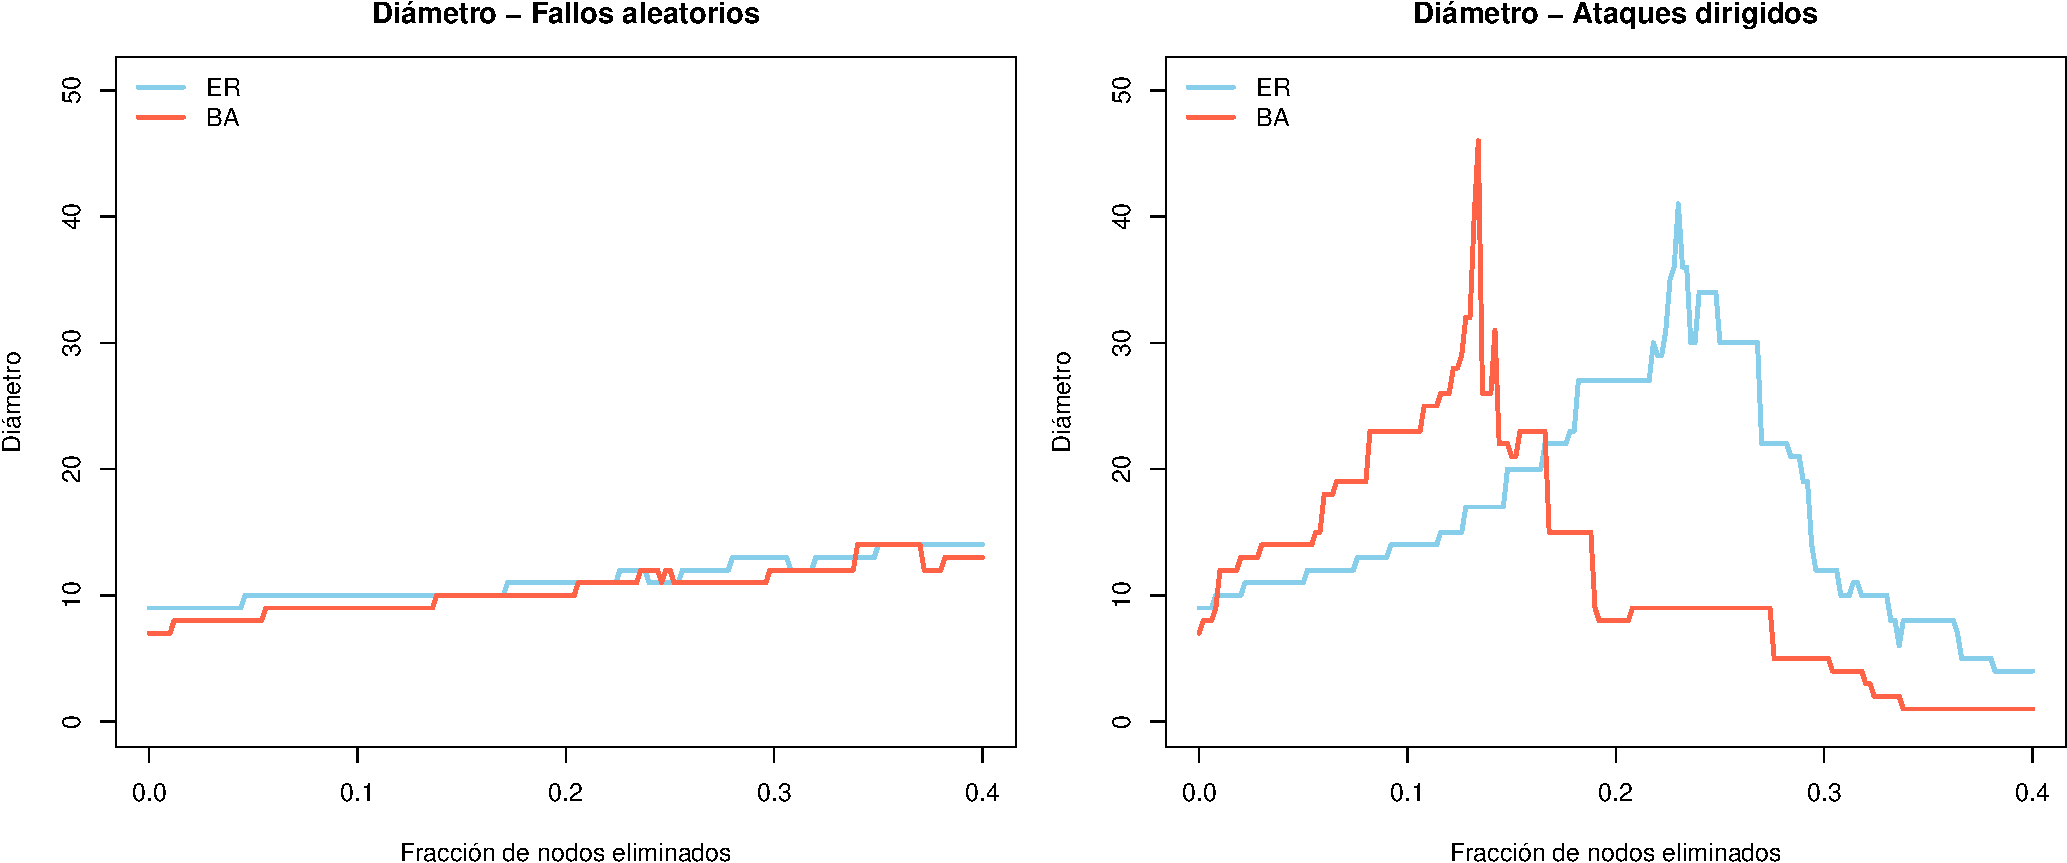
\includegraphics[keepaspectratio]{05-robustez_files/figure-pdf/fig-robustez-diametro-1.pdf}}

}

\caption{\label{fig-robustez-diametro}Evolución del diámetro bajo fallos
(izq.) y ataques (der.)}

\end{figure}%

\section{\texorpdfstring{Incluyendo la red
\emph{Small-World}}{Incluyendo la red Small-World}}\label{incluyendo-la-red-small-world}

Agreguemos una tercera topología para tener una comparación más
completa:

\begin{Shaded}
\begin{Highlighting}[]
\FunctionTok{set.seed}\NormalTok{(}\DecValTok{123}\NormalTok{)}

\NormalTok{g\_sw }\OtherTok{\textless{}{-}} \FunctionTok{sample\_smallworld}\NormalTok{(}\DecValTok{1}\NormalTok{, n, }\AttributeTok{nei =} \DecValTok{2}\NormalTok{, }\AttributeTok{p =} \FloatTok{0.05}\NormalTok{)}
\FunctionTok{V}\NormalTok{(g\_sw)}\SpecialCharTok{$}\NormalTok{name }\OtherTok{\textless{}{-}} \FunctionTok{paste0}\NormalTok{(}\StringTok{"SW\_"}\NormalTok{, }\DecValTok{1}\SpecialCharTok{:}\FunctionTok{vcount}\NormalTok{(g\_sw))}

\FunctionTok{cat}\NormalTok{(}\StringTok{"=== Red Small{-}World ===}\SpecialCharTok{\textbackslash{}n}\StringTok{"}\NormalTok{)}
\end{Highlighting}
\end{Shaded}

\begin{verbatim}
=== Red Small-World ===
\end{verbatim}

\begin{Shaded}
\begin{Highlighting}[]
\FunctionTok{cat}\NormalTok{(}\StringTok{"Nodos:"}\NormalTok{, }\FunctionTok{vcount}\NormalTok{(g\_sw), }\StringTok{" | Aristas:"}\NormalTok{, }\FunctionTok{ecount}\NormalTok{(g\_sw), }\StringTok{"}\SpecialCharTok{\textbackslash{}n}\StringTok{"}\NormalTok{)}
\end{Highlighting}
\end{Shaded}

\begin{verbatim}
Nodos: 500  | Aristas: 1000 
\end{verbatim}

\begin{Shaded}
\begin{Highlighting}[]
\FunctionTok{cat}\NormalTok{(}\StringTok{"Grado medio:"}\NormalTok{, }\FunctionTok{round}\NormalTok{(}\FunctionTok{mean}\NormalTok{(}\FunctionTok{degree}\NormalTok{(g\_sw)), }\DecValTok{2}\NormalTok{), }\StringTok{"}\SpecialCharTok{\textbackslash{}n}\StringTok{"}\NormalTok{)}
\end{Highlighting}
\end{Shaded}

\begin{verbatim}
Grado medio: 4 
\end{verbatim}

\begin{Shaded}
\begin{Highlighting}[]
\FunctionTok{cat}\NormalTok{(}\StringTok{"Grado máximo:"}\NormalTok{, }\FunctionTok{max}\NormalTok{(}\FunctionTok{degree}\NormalTok{(g\_sw)), }\StringTok{"}\SpecialCharTok{\textbackslash{}n}\StringTok{"}\NormalTok{)}
\end{Highlighting}
\end{Shaded}

\begin{verbatim}
Grado máximo: 7 
\end{verbatim}

\begin{Shaded}
\begin{Highlighting}[]
\NormalTok{fallo\_sw  }\OtherTok{\textless{}{-}} \FunctionTok{simular\_fallos}\NormalTok{(g\_sw, }\AttributeTok{fraccion\_eliminar =} \FloatTok{0.4}\NormalTok{)}
\NormalTok{ataque\_sw }\OtherTok{\textless{}{-}} \FunctionTok{simular\_ataques}\NormalTok{(g\_sw, }\AttributeTok{fraccion\_eliminar =} \FloatTok{0.4}\NormalTok{)}
\end{Highlighting}
\end{Shaded}

\begin{Shaded}
\begin{Highlighting}[]
\FunctionTok{par}\NormalTok{(}\AttributeTok{mfrow =} \FunctionTok{c}\NormalTok{(}\DecValTok{1}\NormalTok{, }\DecValTok{2}\NormalTok{), }\AttributeTok{mar =} \FunctionTok{c}\NormalTok{(}\DecValTok{4}\NormalTok{, }\DecValTok{4}\NormalTok{, }\DecValTok{3}\NormalTok{, }\DecValTok{1}\NormalTok{))}

\CommentTok{\# Fallos}
\FunctionTok{plot}\NormalTok{(fallo\_er}\SpecialCharTok{$}\NormalTok{fraccion\_eliminada, fallo\_er}\SpecialCharTok{$}\NormalTok{comp\_gigante,}
     \AttributeTok{type =} \StringTok{"l"}\NormalTok{, }\AttributeTok{lwd =} \FloatTok{2.5}\NormalTok{, }\AttributeTok{col =} \StringTok{"skyblue"}\NormalTok{,}
     \AttributeTok{xlab =} \StringTok{"Fracción eliminada"}\NormalTok{, }\AttributeTok{ylab =} \StringTok{"Componente gigante"}\NormalTok{,}
     \AttributeTok{main =} \StringTok{"Fallos aleatorios"}\NormalTok{, }\AttributeTok{ylim =} \FunctionTok{c}\NormalTok{(}\DecValTok{0}\NormalTok{, }\DecValTok{1}\NormalTok{))}
\FunctionTok{lines}\NormalTok{(fallo\_ba}\SpecialCharTok{$}\NormalTok{fraccion\_eliminada, fallo\_ba}\SpecialCharTok{$}\NormalTok{comp\_gigante,}
      \AttributeTok{lwd =} \FloatTok{2.5}\NormalTok{, }\AttributeTok{col =} \StringTok{"tomato"}\NormalTok{)}
\FunctionTok{lines}\NormalTok{(fallo\_sw}\SpecialCharTok{$}\NormalTok{fraccion\_eliminada, fallo\_sw}\SpecialCharTok{$}\NormalTok{comp\_gigante,}
      \AttributeTok{lwd =} \FloatTok{2.5}\NormalTok{, }\AttributeTok{col =} \StringTok{"mediumpurple"}\NormalTok{)}
\FunctionTok{legend}\NormalTok{(}\StringTok{"topright"}\NormalTok{, }\AttributeTok{legend =} \FunctionTok{c}\NormalTok{(}\StringTok{"ER"}\NormalTok{, }\StringTok{"BA"}\NormalTok{, }\StringTok{"Small{-}world"}\NormalTok{),}
       \AttributeTok{col =} \FunctionTok{c}\NormalTok{(}\StringTok{"skyblue"}\NormalTok{, }\StringTok{"tomato"}\NormalTok{, }\StringTok{"mediumpurple"}\NormalTok{), }\AttributeTok{lwd =} \FloatTok{2.5}\NormalTok{, }\AttributeTok{bty =} \StringTok{"n"}\NormalTok{)}

\CommentTok{\# Ataques}
\FunctionTok{plot}\NormalTok{(ataque\_er}\SpecialCharTok{$}\NormalTok{fraccion\_eliminada, ataque\_er}\SpecialCharTok{$}\NormalTok{comp\_gigante,}
     \AttributeTok{type =} \StringTok{"l"}\NormalTok{, }\AttributeTok{lwd =} \FloatTok{2.5}\NormalTok{, }\AttributeTok{col =} \StringTok{"skyblue"}\NormalTok{,}
     \AttributeTok{xlab =} \StringTok{"Fracción eliminada"}\NormalTok{, }\AttributeTok{ylab =} \StringTok{"Componente gigante"}\NormalTok{,}
     \AttributeTok{main =} \StringTok{"Ataques dirigidos"}\NormalTok{, }\AttributeTok{ylim =} \FunctionTok{c}\NormalTok{(}\DecValTok{0}\NormalTok{, }\DecValTok{1}\NormalTok{))}
\FunctionTok{lines}\NormalTok{(ataque\_ba}\SpecialCharTok{$}\NormalTok{fraccion\_eliminada, ataque\_ba}\SpecialCharTok{$}\NormalTok{comp\_gigante,}
      \AttributeTok{lwd =} \FloatTok{2.5}\NormalTok{, }\AttributeTok{col =} \StringTok{"tomato"}\NormalTok{)}
\FunctionTok{lines}\NormalTok{(ataque\_sw}\SpecialCharTok{$}\NormalTok{fraccion\_eliminada, ataque\_sw}\SpecialCharTok{$}\NormalTok{comp\_gigante,}
      \AttributeTok{lwd =} \FloatTok{2.5}\NormalTok{, }\AttributeTok{col =} \StringTok{"mediumpurple"}\NormalTok{)}
\FunctionTok{legend}\NormalTok{(}\StringTok{"topright"}\NormalTok{, }\AttributeTok{legend =} \FunctionTok{c}\NormalTok{(}\StringTok{"ER"}\NormalTok{, }\StringTok{"BA"}\NormalTok{, }\StringTok{"Small{-}world"}\NormalTok{),}
       \AttributeTok{col =} \FunctionTok{c}\NormalTok{(}\StringTok{"skyblue"}\NormalTok{, }\StringTok{"tomato"}\NormalTok{, }\StringTok{"mediumpurple"}\NormalTok{), }\AttributeTok{lwd =} \FloatTok{2.5}\NormalTok{, }\AttributeTok{bty =} \StringTok{"n"}\NormalTok{)}
\end{Highlighting}
\end{Shaded}

\begin{figure}[H]

\centering{

\pandocbounded{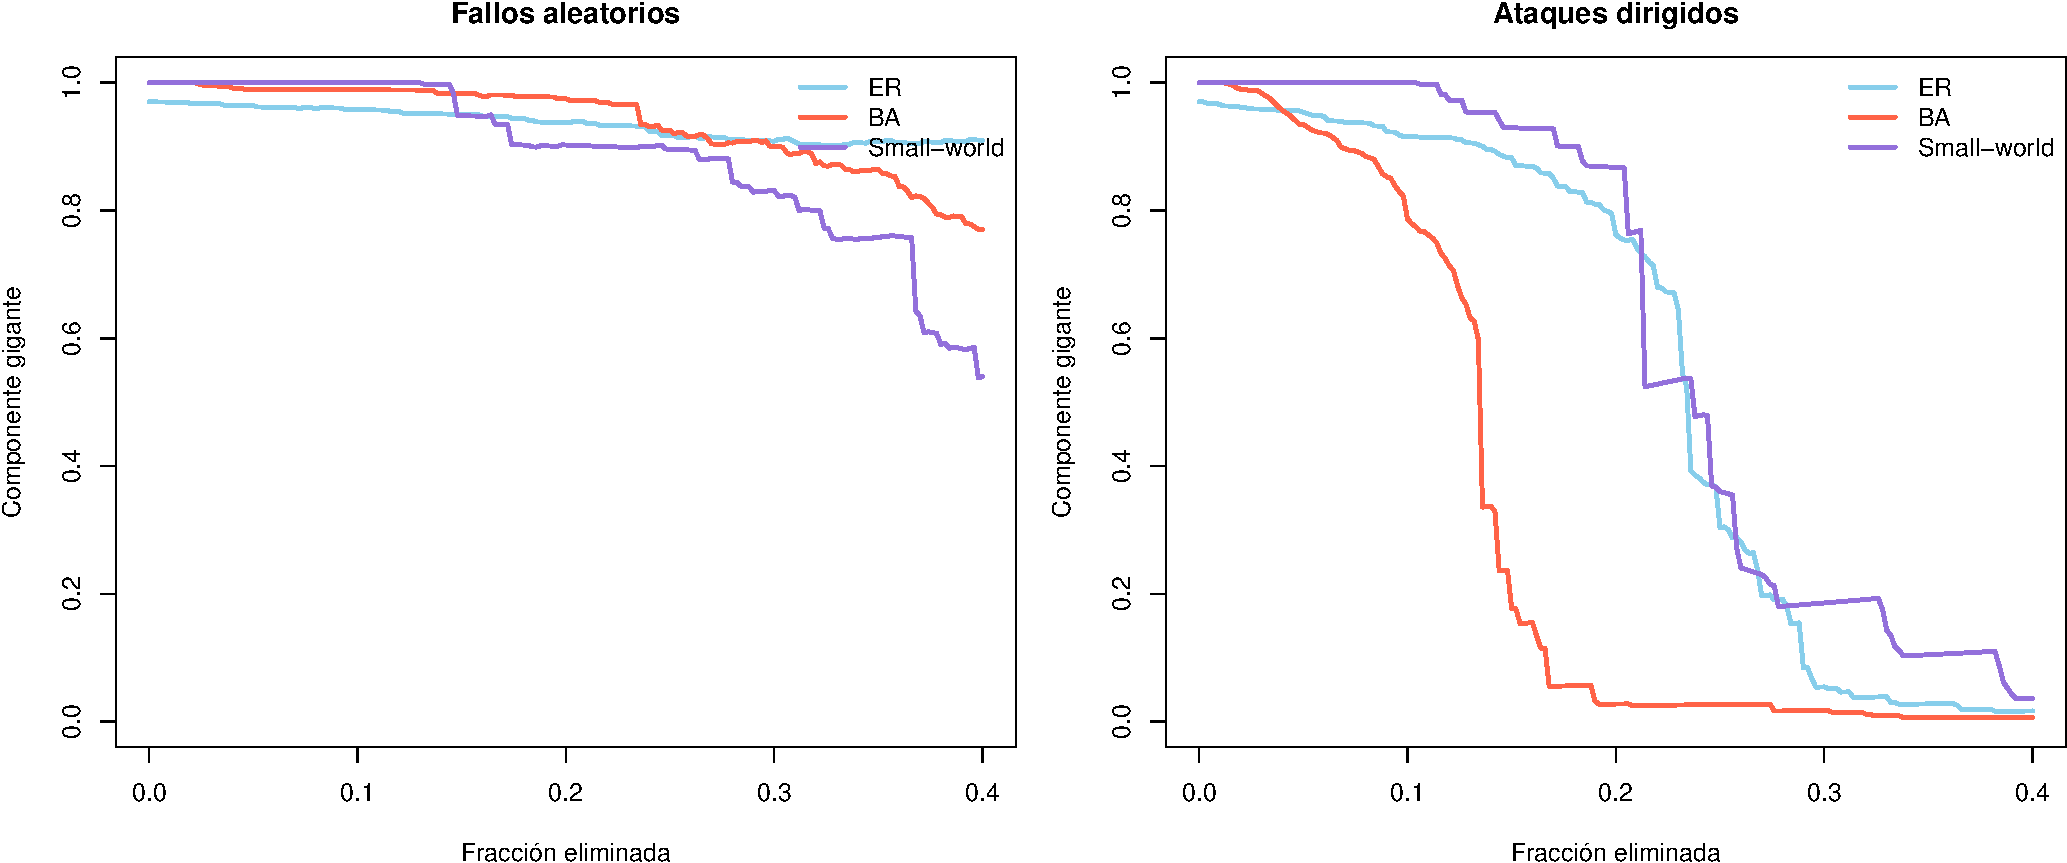
\includegraphics[keepaspectratio]{05-robustez_files/figure-pdf/fig-robustez-tres-redes-1.pdf}}

}

\caption{\label{fig-robustez-tres-redes}Componente gigante bajo fallos y
ataques para tres topologías}

\end{figure}%

\section{Tabla resumen de robustez}\label{tabla-resumen-de-robustez}

\begin{Shaded}
\begin{Highlighting}[]
\CommentTok{\# Fracción de nodos que se deben eliminar para que el comp. gigante baje del 50\%}
\NormalTok{umbral\_fragmentacion }\OtherTok{\textless{}{-}} \ControlFlowTok{function}\NormalTok{(resultados, }\AttributeTok{umbral =} \FloatTok{0.5}\NormalTok{) \{}
\NormalTok{  idx }\OtherTok{\textless{}{-}} \FunctionTok{which}\NormalTok{(resultados}\SpecialCharTok{$}\NormalTok{comp\_gigante }\SpecialCharTok{\textless{}}\NormalTok{ umbral)}
  \ControlFlowTok{if}\NormalTok{ (}\FunctionTok{length}\NormalTok{(idx) }\SpecialCharTok{==} \DecValTok{0}\NormalTok{) }\FunctionTok{return}\NormalTok{(}\StringTok{"\textgreater{} 40\%"}\NormalTok{)}
  \FunctionTok{paste0}\NormalTok{(}\FunctionTok{round}\NormalTok{(resultados}\SpecialCharTok{$}\NormalTok{fraccion\_eliminada[}\FunctionTok{min}\NormalTok{(idx)] }\SpecialCharTok{*} \DecValTok{100}\NormalTok{, }\DecValTok{1}\NormalTok{), }\StringTok{"\%"}\NormalTok{)}
\NormalTok{\}}

\NormalTok{resumen\_rob }\OtherTok{\textless{}{-}} \FunctionTok{data.frame}\NormalTok{(}
  \AttributeTok{Red =} \FunctionTok{c}\NormalTok{(}\StringTok{"Erdős–Rényi"}\NormalTok{, }\StringTok{"Barabási–Albert"}\NormalTok{, }\StringTok{"Small{-}world"}\NormalTok{),}
  \AttributeTok{Fallo\_50 =} \FunctionTok{c}\NormalTok{(}
    \FunctionTok{umbral\_fragmentacion}\NormalTok{(fallo\_er),}
    \FunctionTok{umbral\_fragmentacion}\NormalTok{(fallo\_ba),}
    \FunctionTok{umbral\_fragmentacion}\NormalTok{(fallo\_sw)}
\NormalTok{  ),}
  \AttributeTok{Ataque\_50 =} \FunctionTok{c}\NormalTok{(}
    \FunctionTok{umbral\_fragmentacion}\NormalTok{(ataque\_er),}
    \FunctionTok{umbral\_fragmentacion}\NormalTok{(ataque\_ba),}
    \FunctionTok{umbral\_fragmentacion}\NormalTok{(ataque\_sw)}
\NormalTok{  )}
\NormalTok{)}

\NormalTok{knitr}\SpecialCharTok{::}\FunctionTok{kable}\NormalTok{(resumen\_rob,}
             \AttributeTok{caption =} \StringTok{"Fracción de nodos a eliminar para fragmentar la red (comp. gigante \textless{} 50\%)"}\NormalTok{,}
             \AttributeTok{col.names =} \FunctionTok{c}\NormalTok{(}\StringTok{"Red"}\NormalTok{, }\StringTok{"Fallos aleatorios"}\NormalTok{, }\StringTok{"Ataques dirigidos"}\NormalTok{))}
\end{Highlighting}
\end{Shaded}

\begin{longtable}[]{@{}lll@{}}
\caption{Fracción de nodos a eliminar para fragmentar la red (comp.
gigante \textless{} 50\%)}\tabularnewline
\toprule\noalign{}
Red & Fallos aleatorios & Ataques dirigidos \\
\midrule\noalign{}
\endfirsthead
\toprule\noalign{}
Red & Fallos aleatorios & Ataques dirigidos \\
\midrule\noalign{}
\endhead
\bottomrule\noalign{}
\endlastfoot
Erdős--Rényi & \textgreater{} 40\% & 23.6\% \\
Barabási--Albert & \textgreater{} 40\% & 13.6\% \\
Small-world & \textgreater{} 40\% & 23.8\% \\
\end{longtable}

\section{Visualización del proceso de
fragmentación}\label{visualizaciuxf3n-del-proceso-de-fragmentaciuxf3n}

Veamos cómo luce la red BA antes, durante y después de un ataque
dirigido:

\begin{Shaded}
\begin{Highlighting}[]
\FunctionTok{set.seed}\NormalTok{(}\DecValTok{42}\NormalTok{)}
\NormalTok{g\_vis }\OtherTok{\textless{}{-}} \FunctionTok{sample\_pa}\NormalTok{(}\DecValTok{100}\NormalTok{, }\AttributeTok{m =} \DecValTok{2}\NormalTok{, }\AttributeTok{directed =} \ConstantTok{FALSE}\NormalTok{)}
\FunctionTok{V}\NormalTok{(g\_vis)}\SpecialCharTok{$}\NormalTok{name }\OtherTok{\textless{}{-}} \FunctionTok{paste0}\NormalTok{(}\StringTok{"v"}\NormalTok{, }\DecValTok{1}\SpecialCharTok{:}\DecValTok{100}\NormalTok{)}

\CommentTok{\# Layout fijo}
\NormalTok{lay\_vis }\OtherTok{\textless{}{-}} \FunctionTok{layout\_with\_fr}\NormalTok{(g\_vis)}

\FunctionTok{par}\NormalTok{(}\AttributeTok{mfrow =} \FunctionTok{c}\NormalTok{(}\DecValTok{1}\NormalTok{, }\DecValTok{3}\NormalTok{), }\AttributeTok{mar =} \FunctionTok{c}\NormalTok{(}\DecValTok{1}\NormalTok{, }\DecValTok{1}\NormalTok{, }\DecValTok{3}\NormalTok{, }\DecValTok{1}\NormalTok{))}

\CommentTok{\# Estado original}
\FunctionTok{V}\NormalTok{(g\_vis)}\SpecialCharTok{$}\NormalTok{color }\OtherTok{\textless{}{-}} \StringTok{"skyblue"}
\FunctionTok{V}\NormalTok{(g\_vis)}\SpecialCharTok{$}\NormalTok{size }\OtherTok{\textless{}{-}} \FunctionTok{degree}\NormalTok{(g\_vis) }\SpecialCharTok{*} \FloatTok{0.8} \SpecialCharTok{+} \DecValTok{3}
\FunctionTok{plot}\NormalTok{(g\_vis, }\AttributeTok{layout =}\NormalTok{ lay\_vis, }\AttributeTok{vertex.label =} \ConstantTok{NA}\NormalTok{,}
     \AttributeTok{edge.color =} \FunctionTok{adjustcolor}\NormalTok{(}\StringTok{"gray50"}\NormalTok{, }\FloatTok{0.4}\NormalTok{),}
     \AttributeTok{main =} \FunctionTok{paste0}\NormalTok{(}\StringTok{"Original}\SpecialCharTok{\textbackslash{}n}\StringTok{("}\NormalTok{, }\FunctionTok{vcount}\NormalTok{(g\_vis), }\StringTok{" nodos, "}\NormalTok{, }
                   \FunctionTok{components}\NormalTok{(g\_vis)}\SpecialCharTok{$}\NormalTok{no, }\StringTok{" comp.)"}\NormalTok{))}

\CommentTok{\# Eliminar los 5 hubs más conectados}
\NormalTok{g\_vis2 }\OtherTok{\textless{}{-}}\NormalTok{ g\_vis}
\ControlFlowTok{for}\NormalTok{ (j }\ControlFlowTok{in} \DecValTok{1}\SpecialCharTok{:}\DecValTok{5}\NormalTok{) \{}
\NormalTok{  hub }\OtherTok{\textless{}{-}} \FunctionTok{V}\NormalTok{(g\_vis2)}\SpecialCharTok{$}\NormalTok{name[}\FunctionTok{which.max}\NormalTok{(}\FunctionTok{degree}\NormalTok{(g\_vis2))]}
\NormalTok{  g\_vis2 }\OtherTok{\textless{}{-}} \FunctionTok{delete\_vertices}\NormalTok{(g\_vis2, hub)}
\NormalTok{\}}
\FunctionTok{plot}\NormalTok{(g\_vis2, }\AttributeTok{vertex.label =} \ConstantTok{NA}\NormalTok{,}
     \AttributeTok{vertex.size =} \FunctionTok{degree}\NormalTok{(g\_vis2) }\SpecialCharTok{*} \FloatTok{0.8} \SpecialCharTok{+} \DecValTok{3}\NormalTok{,}
     \AttributeTok{vertex.color =} \StringTok{"gold"}\NormalTok{,}
     \AttributeTok{edge.color =} \FunctionTok{adjustcolor}\NormalTok{(}\StringTok{"gray50"}\NormalTok{, }\FloatTok{0.4}\NormalTok{),}
     \AttributeTok{main =} \FunctionTok{paste0}\NormalTok{(}\StringTok{"Tras 5 ataques}\SpecialCharTok{\textbackslash{}n}\StringTok{("}\NormalTok{, }\FunctionTok{vcount}\NormalTok{(g\_vis2), }\StringTok{" nodos, "}\NormalTok{, }
                   \FunctionTok{components}\NormalTok{(g\_vis2)}\SpecialCharTok{$}\NormalTok{no, }\StringTok{" comp.)"}\NormalTok{))}

\CommentTok{\# Eliminar 5 hubs más (10 total)}
\ControlFlowTok{for}\NormalTok{ (j }\ControlFlowTok{in} \DecValTok{1}\SpecialCharTok{:}\DecValTok{5}\NormalTok{) \{}
\NormalTok{  hub }\OtherTok{\textless{}{-}} \FunctionTok{V}\NormalTok{(g\_vis2)}\SpecialCharTok{$}\NormalTok{name[}\FunctionTok{which.max}\NormalTok{(}\FunctionTok{degree}\NormalTok{(g\_vis2))]}
\NormalTok{  g\_vis2 }\OtherTok{\textless{}{-}} \FunctionTok{delete\_vertices}\NormalTok{(g\_vis2, hub)}
\NormalTok{\}}
\FunctionTok{plot}\NormalTok{(g\_vis2, }\AttributeTok{vertex.label =} \ConstantTok{NA}\NormalTok{,}
     \AttributeTok{vertex.size =} \FunctionTok{degree}\NormalTok{(g\_vis2) }\SpecialCharTok{*} \FloatTok{0.8} \SpecialCharTok{+} \DecValTok{3}\NormalTok{,}
     \AttributeTok{vertex.color =} \StringTok{"tomato"}\NormalTok{,}
     \AttributeTok{edge.color =} \FunctionTok{adjustcolor}\NormalTok{(}\StringTok{"gray50"}\NormalTok{, }\FloatTok{0.4}\NormalTok{),}
     \AttributeTok{main =} \FunctionTok{paste0}\NormalTok{(}\StringTok{"Tras 10 ataques}\SpecialCharTok{\textbackslash{}n}\StringTok{("}\NormalTok{, }\FunctionTok{vcount}\NormalTok{(g\_vis2), }\StringTok{" nodos, "}\NormalTok{, }
                   \FunctionTok{components}\NormalTok{(g\_vis2)}\SpecialCharTok{$}\NormalTok{no, }\StringTok{" comp.)"}\NormalTok{))}
\end{Highlighting}
\end{Shaded}

\begin{figure}[H]

\centering{

\pandocbounded{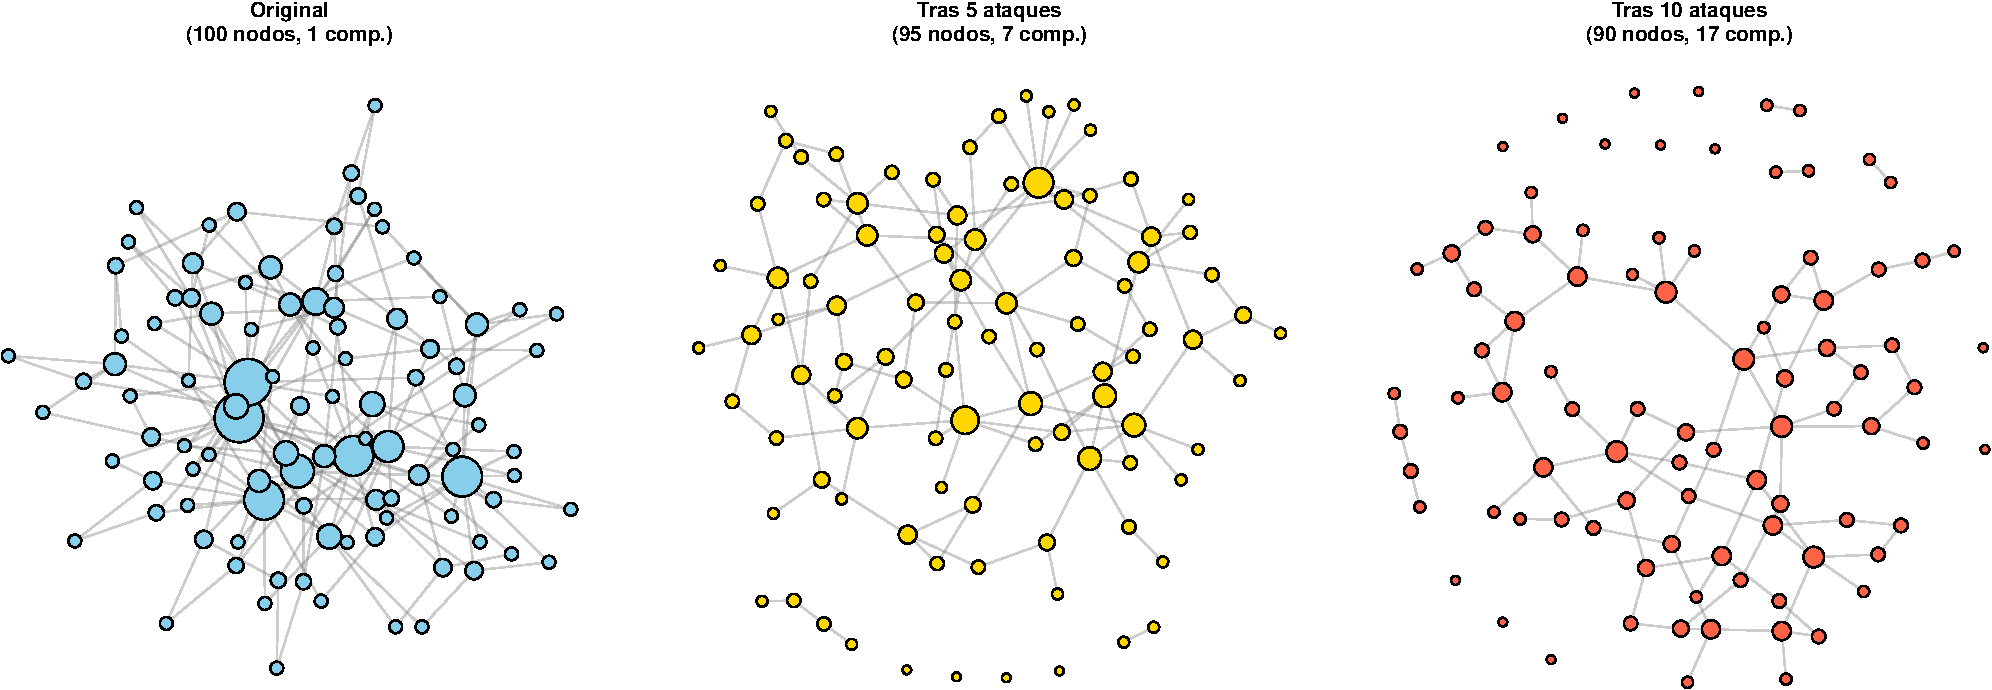
\includegraphics[keepaspectratio]{05-robustez_files/figure-pdf/fig-fragmentacion-visual-1.pdf}}

}

\caption{\label{fig-fragmentacion-visual}Fragmentación progresiva de una
red BA (100 nodos) bajo ataque dirigido}

\end{figure}%

\section{Múltiples realizaciones: promediar la
incertidumbre}\label{muxfaltiples-realizaciones-promediar-la-incertidumbre}

Una sola simulación puede dar resultados atípicos. Para tener
conclusiones robustas, repetimos el experimento múltiples veces y
promediamos.

\begin{Shaded}
\begin{Highlighting}[]
\FunctionTok{set.seed}\NormalTok{(}\DecValTok{42}\NormalTok{)}

\NormalTok{n\_reps }\OtherTok{\textless{}{-}} \DecValTok{10}
\NormalTok{n\_red }\OtherTok{\textless{}{-}} \DecValTok{200}
\NormalTok{fraccion }\OtherTok{\textless{}{-}} \FloatTok{0.5}
\NormalTok{n\_elim }\OtherTok{\textless{}{-}} \FunctionTok{floor}\NormalTok{(n\_red }\SpecialCharTok{*}\NormalTok{ fraccion)}

\CommentTok{\# Matriz para almacenar resultados}
\NormalTok{resultados\_mat }\OtherTok{\textless{}{-}} \FunctionTok{matrix}\NormalTok{(}\ConstantTok{NA}\NormalTok{, }\AttributeTok{nrow =}\NormalTok{ n\_elim }\SpecialCharTok{+} \DecValTok{1}\NormalTok{, }\AttributeTok{ncol =}\NormalTok{ n\_reps)}

\ControlFlowTok{for}\NormalTok{ (r }\ControlFlowTok{in} \DecValTok{1}\SpecialCharTok{:}\NormalTok{n\_reps) \{}
\NormalTok{  g\_rep }\OtherTok{\textless{}{-}} \FunctionTok{sample\_pa}\NormalTok{(n\_red, }\AttributeTok{m =} \DecValTok{2}\NormalTok{, }\AttributeTok{directed =} \ConstantTok{FALSE}\NormalTok{)}
  \FunctionTok{V}\NormalTok{(g\_rep)}\SpecialCharTok{$}\NormalTok{name }\OtherTok{\textless{}{-}} \FunctionTok{paste0}\NormalTok{(}\StringTok{"v"}\NormalTok{, }\DecValTok{1}\SpecialCharTok{:}\FunctionTok{vcount}\NormalTok{(g\_rep))}
  
  \CommentTok{\# Orden aleatorio de eliminación}
\NormalTok{  orden }\OtherTok{\textless{}{-}} \FunctionTok{sample}\NormalTok{(}\FunctionTok{V}\NormalTok{(g\_rep)}\SpecialCharTok{$}\NormalTok{name, n\_elim)}
\NormalTok{  g\_temp }\OtherTok{\textless{}{-}}\NormalTok{ g\_rep}
\NormalTok{  resultados\_mat[}\DecValTok{1}\NormalTok{, r] }\OtherTok{\textless{}{-}} \FunctionTok{tamano\_gigante}\NormalTok{(g\_temp)}
  
  \ControlFlowTok{for}\NormalTok{ (i }\ControlFlowTok{in} \DecValTok{1}\SpecialCharTok{:}\NormalTok{n\_elim) \{}
\NormalTok{    g\_temp }\OtherTok{\textless{}{-}} \FunctionTok{delete\_vertices}\NormalTok{(g\_temp, orden[i])}
\NormalTok{    resultados\_mat[i }\SpecialCharTok{+} \DecValTok{1}\NormalTok{, r] }\OtherTok{\textless{}{-}} \FunctionTok{tamano\_gigante}\NormalTok{(g\_temp)}
\NormalTok{  \}}
\NormalTok{\}}

\CommentTok{\# Calcular media y banda}
\NormalTok{frac\_x }\OtherTok{\textless{}{-}}\NormalTok{ (}\DecValTok{0}\SpecialCharTok{:}\NormalTok{n\_elim) }\SpecialCharTok{/}\NormalTok{ n\_red}
\NormalTok{media }\OtherTok{\textless{}{-}} \FunctionTok{rowMeans}\NormalTok{(resultados\_mat)}
\NormalTok{desv }\OtherTok{\textless{}{-}} \FunctionTok{apply}\NormalTok{(resultados\_mat, }\DecValTok{1}\NormalTok{, sd)}

\FunctionTok{plot}\NormalTok{(frac\_x, media,}
     \AttributeTok{type =} \StringTok{"l"}\NormalTok{, }\AttributeTok{lwd =} \DecValTok{3}\NormalTok{, }\AttributeTok{col =} \StringTok{"tomato"}\NormalTok{,}
     \AttributeTok{xlab =} \StringTok{"Fracción de nodos eliminados"}\NormalTok{,}
     \AttributeTok{ylab =} \StringTok{"Componente gigante (media ± 1 DE)"}\NormalTok{,}
     \AttributeTok{main =} \FunctionTok{paste}\NormalTok{(}\StringTok{"Fallos aleatorios — Red BA (n=200),"}\NormalTok{, n\_reps, }\StringTok{"realizaciones"}\NormalTok{),}
     \AttributeTok{ylim =} \FunctionTok{c}\NormalTok{(}\DecValTok{0}\NormalTok{, }\DecValTok{1}\NormalTok{))}

\CommentTok{\# Banda de ± 1 desviación estándar}
\FunctionTok{polygon}\NormalTok{(}\FunctionTok{c}\NormalTok{(frac\_x, }\FunctionTok{rev}\NormalTok{(frac\_x)),}
        \FunctionTok{c}\NormalTok{(media }\SpecialCharTok{+}\NormalTok{ desv, }\FunctionTok{rev}\NormalTok{(media }\SpecialCharTok{{-}}\NormalTok{ desv)),}
        \AttributeTok{col =} \FunctionTok{adjustcolor}\NormalTok{(}\StringTok{"tomato"}\NormalTok{, }\FloatTok{0.2}\NormalTok{), }\AttributeTok{border =} \ConstantTok{NA}\NormalTok{)}

\FunctionTok{lines}\NormalTok{(frac\_x, media, }\AttributeTok{lwd =} \DecValTok{3}\NormalTok{, }\AttributeTok{col =} \StringTok{"tomato"}\NormalTok{)}
\FunctionTok{legend}\NormalTok{(}\StringTok{"topright"}\NormalTok{, }
       \AttributeTok{legend =} \FunctionTok{c}\NormalTok{(}\StringTok{"Media"}\NormalTok{, }\StringTok{"± 1 DE"}\NormalTok{),}
       \AttributeTok{col =} \FunctionTok{c}\NormalTok{(}\StringTok{"tomato"}\NormalTok{, }\FunctionTok{adjustcolor}\NormalTok{(}\StringTok{"tomato"}\NormalTok{, }\FloatTok{0.3}\NormalTok{)),}
       \AttributeTok{lwd =} \FunctionTok{c}\NormalTok{(}\DecValTok{3}\NormalTok{, }\DecValTok{10}\NormalTok{), }\AttributeTok{bty =} \StringTok{"n"}\NormalTok{)}
\end{Highlighting}
\end{Shaded}

\begin{figure}[H]

\centering{

\pandocbounded{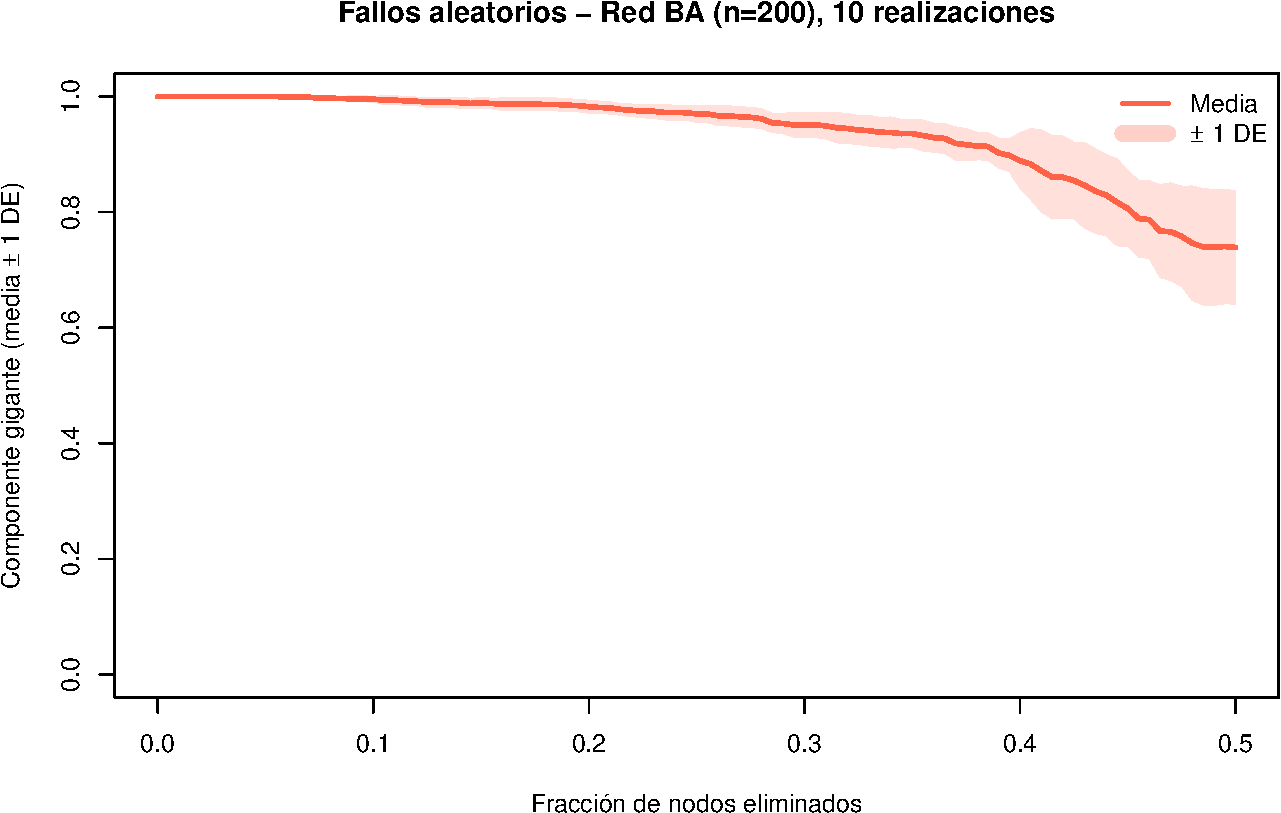
\includegraphics[keepaspectratio]{05-robustez_files/figure-pdf/fig-multiples-realizaciones-1.pdf}}

}

\caption{\label{fig-multiples-realizaciones}Componente gigante promedio
(10 realizaciones) bajo fallos aleatorios para redes BA de 200 nodos}

\end{figure}%

\begin{tcolorbox}[enhanced jigsaw, colback=white, toprule=.15mm, title=\textcolor{quarto-callout-tip-color}{\faLightbulb}\hspace{0.5em}{💡 Concepto clave}, titlerule=0mm, colframe=quarto-callout-tip-color-frame, breakable, opacitybacktitle=0.6, toptitle=1mm, left=2mm, bottomrule=.15mm, bottomtitle=1mm, arc=.35mm, rightrule=.15mm, leftrule=.75mm, opacityback=0, coltitle=black, colbacktitle=quarto-callout-tip-color!10!white]

La \textbf{banda de variabilidad} (sombreada) muestra cuánto varían los
resultados entre realizaciones. Si la banda es estrecha, el resultado es
robusto y reproducible. Siempre que hagas simulaciones estocásticas,
reporta la variabilidad, no solo la media.

\end{tcolorbox}

\section{Ejercicios}\label{ejercicios-4}

\subsection*{Ejercicios resueltos}\label{ejercicios-resueltos-4}
\addcontentsline{toc}{subsection}{Ejercicios resueltos}

\textbf{Ejercicio resuelto 1:} Genera las siguientes cuatro redes. Para
cada una, elimina aleatoriamente 1/100 de sus nodos 10 veces
consecutivas. En cada paso, calcula la distancia media y el diámetro.
Presenta los resultados en una tabla.

\begin{itemize}
\tightlist
\item
  \texttt{g100}: Barabási--Albert con 100 nodos
\item
  \texttt{g1K}: Barabási--Albert con 1000 nodos
\item
  \texttt{g\_er}: Erdős--Rényi con 1000 nodos y \(p = 0.20\)
\item
  \texttt{g\_sw}: \emph{Small-world} con 1000 nodos, \texttt{nei\ =\ 3},
  \(p = 0.2\)
\end{itemize}

\begin{tcolorbox}[enhanced jigsaw, colback=white, toprule=.15mm, title=\textcolor{quarto-callout-tip-color}{\faLightbulb}\hspace{0.5em}{📝 Solución}, titlerule=0mm, colframe=quarto-callout-tip-color-frame, breakable, opacitybacktitle=0.6, toptitle=1mm, left=2mm, bottomrule=.15mm, bottomtitle=1mm, arc=.35mm, rightrule=.15mm, leftrule=.75mm, opacityback=0, coltitle=black, colbacktitle=quarto-callout-tip-color!10!white]

\textbf{Paso 1:} Crear las redes.

\begin{Shaded}
\begin{Highlighting}[]
\FunctionTok{set.seed}\NormalTok{(}\DecValTok{42}\NormalTok{)}

\NormalTok{redes\_ej }\OtherTok{\textless{}{-}} \FunctionTok{list}\NormalTok{(}
  \AttributeTok{BA\_100  =} \FunctionTok{sample\_pa}\NormalTok{(}\DecValTok{100}\NormalTok{, }\AttributeTok{directed =} \ConstantTok{FALSE}\NormalTok{),}
  \AttributeTok{BA\_1000 =} \FunctionTok{sample\_pa}\NormalTok{(}\DecValTok{1000}\NormalTok{, }\AttributeTok{directed =} \ConstantTok{FALSE}\NormalTok{),}
  \AttributeTok{ER\_1000 =} \FunctionTok{sample\_gnp}\NormalTok{(}\DecValTok{1000}\NormalTok{, }\FloatTok{0.20}\NormalTok{),}
  \AttributeTok{SW\_1000 =} \FunctionTok{sample\_smallworld}\NormalTok{(}\DecValTok{1}\NormalTok{, }\DecValTok{1000}\NormalTok{, }\AttributeTok{nei =} \DecValTok{3}\NormalTok{, }\AttributeTok{p =} \FloatTok{0.2}\NormalTok{)}
\NormalTok{)}

\CommentTok{\# Asignar nombres a los nodos}
\ControlFlowTok{for}\NormalTok{ (nombre }\ControlFlowTok{in} \FunctionTok{names}\NormalTok{(redes\_ej)) \{}
  \FunctionTok{V}\NormalTok{(redes\_ej[[nombre]])}\SpecialCharTok{$}\NormalTok{name }\OtherTok{\textless{}{-}} \FunctionTok{paste0}\NormalTok{(}\StringTok{"n"}\NormalTok{, }\DecValTok{1}\SpecialCharTok{:}\FunctionTok{vcount}\NormalTok{(redes\_ej[[nombre]]))}
\NormalTok{\}}
\end{Highlighting}
\end{Shaded}

\textbf{Paso 2:} Simular eliminación de 1/100 de los nodos, 10 veces
consecutivas.

\begin{Shaded}
\begin{Highlighting}[]
\NormalTok{resultados\_ej1 }\OtherTok{\textless{}{-}} \FunctionTok{list}\NormalTok{()}

\ControlFlowTok{for}\NormalTok{ (nombre }\ControlFlowTok{in} \FunctionTok{names}\NormalTok{(redes\_ej)) \{}
\NormalTok{  g }\OtherTok{\textless{}{-}}\NormalTok{ redes\_ej[[nombre]]}
\NormalTok{  n }\OtherTok{\textless{}{-}} \FunctionTok{vcount}\NormalTok{(g)}
\NormalTok{  n\_elim\_paso }\OtherTok{\textless{}{-}} \FunctionTok{max}\NormalTok{(}\DecValTok{1}\NormalTok{, }\FunctionTok{floor}\NormalTok{(n }\SpecialCharTok{/} \DecValTok{100}\NormalTok{))  }\CommentTok{\# 1/100 de los nodos}
  
\NormalTok{  registros }\OtherTok{\textless{}{-}} \FunctionTok{data.frame}\NormalTok{(}
    \AttributeTok{paso =} \DecValTok{0}\SpecialCharTok{:}\DecValTok{10}\NormalTok{,}
    \AttributeTok{nodos\_restantes =} \FunctionTok{numeric}\NormalTok{(}\DecValTok{11}\NormalTok{),}
    \AttributeTok{dist\_media =} \FunctionTok{numeric}\NormalTok{(}\DecValTok{11}\NormalTok{),}
    \AttributeTok{diametro =} \FunctionTok{numeric}\NormalTok{(}\DecValTok{11}\NormalTok{)}
\NormalTok{  )}
  
\NormalTok{  g\_temp }\OtherTok{\textless{}{-}}\NormalTok{ g}
  \ControlFlowTok{for}\NormalTok{ (paso }\ControlFlowTok{in} \DecValTok{0}\SpecialCharTok{:}\DecValTok{10}\NormalTok{) \{}
    \ControlFlowTok{if}\NormalTok{ (paso }\SpecialCharTok{\textgreater{}} \DecValTok{0}\NormalTok{) \{}
      \CommentTok{\# Eliminar 1/100 nodos al azar}
\NormalTok{      n\_actual }\OtherTok{\textless{}{-}} \FunctionTok{vcount}\NormalTok{(g\_temp)}
\NormalTok{      n\_quitar }\OtherTok{\textless{}{-}} \FunctionTok{min}\NormalTok{(n\_elim\_paso, n\_actual }\SpecialCharTok{{-}} \DecValTok{1}\NormalTok{)}
\NormalTok{      victimas }\OtherTok{\textless{}{-}} \FunctionTok{sample}\NormalTok{(}\FunctionTok{V}\NormalTok{(g\_temp)}\SpecialCharTok{$}\NormalTok{name, n\_quitar)}
\NormalTok{      g\_temp }\OtherTok{\textless{}{-}} \FunctionTok{delete\_vertices}\NormalTok{(g\_temp, victimas)}
\NormalTok{    \}}
\NormalTok{    registros}\SpecialCharTok{$}\NormalTok{nodos\_restantes[paso }\SpecialCharTok{+} \DecValTok{1}\NormalTok{] }\OtherTok{\textless{}{-}} \FunctionTok{vcount}\NormalTok{(g\_temp)}
\NormalTok{    registros}\SpecialCharTok{$}\NormalTok{dist\_media[paso }\SpecialCharTok{+} \DecValTok{1}\NormalTok{] }\OtherTok{\textless{}{-}} \FunctionTok{round}\NormalTok{(}\FunctionTok{mean\_distance}\NormalTok{(g\_temp), }\DecValTok{3}\NormalTok{)}
\NormalTok{    registros}\SpecialCharTok{$}\NormalTok{diametro[paso }\SpecialCharTok{+} \DecValTok{1}\NormalTok{] }\OtherTok{\textless{}{-}} \FunctionTok{diameter}\NormalTok{(g\_temp)}
\NormalTok{  \}}
  
\NormalTok{  resultados\_ej1[[nombre]] }\OtherTok{\textless{}{-}}\NormalTok{ registros}
\NormalTok{\}}
\end{Highlighting}
\end{Shaded}

\textbf{Paso 3:} Mostrar la tabla resumen (valores finales tras 10
rondas).

\begin{Shaded}
\begin{Highlighting}[]
\NormalTok{resumen\_final }\OtherTok{\textless{}{-}} \FunctionTok{data.frame}\NormalTok{(}
  \AttributeTok{Red =} \FunctionTok{names}\NormalTok{(redes\_ej),}
  \AttributeTok{N\_original =} \FunctionTok{sapply}\NormalTok{(redes\_ej, vcount),}
  \AttributeTok{N\_final =} \FunctionTok{sapply}\NormalTok{(resultados\_ej1, }\ControlFlowTok{function}\NormalTok{(r) r}\SpecialCharTok{$}\NormalTok{nodos\_restantes[}\DecValTok{11}\NormalTok{]),}
  \AttributeTok{Dist\_media\_inicio =} \FunctionTok{sapply}\NormalTok{(resultados\_ej1, }\ControlFlowTok{function}\NormalTok{(r) r}\SpecialCharTok{$}\NormalTok{dist\_media[}\DecValTok{1}\NormalTok{]),}
  \AttributeTok{Dist\_media\_final =} \FunctionTok{sapply}\NormalTok{(resultados\_ej1, }\ControlFlowTok{function}\NormalTok{(r) r}\SpecialCharTok{$}\NormalTok{dist\_media[}\DecValTok{11}\NormalTok{]),}
\NormalTok{  Diámetro}\AttributeTok{\_inicio =} \FunctionTok{sapply}\NormalTok{(resultados\_ej1, }\ControlFlowTok{function}\NormalTok{(r) r}\SpecialCharTok{$}\NormalTok{diametro[}\DecValTok{1}\NormalTok{]),}
\NormalTok{  Diámetro}\AttributeTok{\_final =} \FunctionTok{sapply}\NormalTok{(resultados\_ej1, }\ControlFlowTok{function}\NormalTok{(r) r}\SpecialCharTok{$}\NormalTok{diametro[}\DecValTok{11}\NormalTok{])}
\NormalTok{)}

\NormalTok{knitr}\SpecialCharTok{::}\FunctionTok{kable}\NormalTok{(resumen\_final,}
             \AttributeTok{caption =} \StringTok{"Efecto de eliminar 1/100 nodos aleatorios en 10 rondas"}\NormalTok{,}
             \AttributeTok{col.names =} \FunctionTok{c}\NormalTok{(}\StringTok{"Red"}\NormalTok{, }\StringTok{"N original"}\NormalTok{, }\StringTok{"N final"}\NormalTok{, }
                           \StringTok{"Dist. media (inicio)"}\NormalTok{, }\StringTok{"Dist. media (final)"}\NormalTok{,}
                           \StringTok{"Diámetro (inicio)"}\NormalTok{, }\StringTok{"Diámetro (final)"}\NormalTok{))}
\end{Highlighting}
\end{Shaded}

\begin{longtable}[]{@{}
  >{\raggedright\arraybackslash}p{(\linewidth - 14\tabcolsep) * \real{0.0721}}
  >{\raggedright\arraybackslash}p{(\linewidth - 14\tabcolsep) * \real{0.0721}}
  >{\raggedleft\arraybackslash}p{(\linewidth - 14\tabcolsep) * \real{0.0991}}
  >{\raggedleft\arraybackslash}p{(\linewidth - 14\tabcolsep) * \real{0.0721}}
  >{\raggedleft\arraybackslash}p{(\linewidth - 14\tabcolsep) * \real{0.1892}}
  >{\raggedleft\arraybackslash}p{(\linewidth - 14\tabcolsep) * \real{0.1802}}
  >{\raggedleft\arraybackslash}p{(\linewidth - 14\tabcolsep) * \real{0.1622}}
  >{\raggedleft\arraybackslash}p{(\linewidth - 14\tabcolsep) * \real{0.1532}}@{}}
\caption{Efecto de eliminar 1/100 nodos aleatorios en 10
rondas}\tabularnewline
\toprule\noalign{}
\begin{minipage}[b]{\linewidth}\raggedright
\end{minipage} & \begin{minipage}[b]{\linewidth}\raggedright
Red
\end{minipage} & \begin{minipage}[b]{\linewidth}\raggedleft
N original
\end{minipage} & \begin{minipage}[b]{\linewidth}\raggedleft
N final
\end{minipage} & \begin{minipage}[b]{\linewidth}\raggedleft
Dist. media (inicio)
\end{minipage} & \begin{minipage}[b]{\linewidth}\raggedleft
Dist. media (final)
\end{minipage} & \begin{minipage}[b]{\linewidth}\raggedleft
Diámetro (inicio)
\end{minipage} & \begin{minipage}[b]{\linewidth}\raggedleft
Diámetro (final)
\end{minipage} \\
\midrule\noalign{}
\endfirsthead
\toprule\noalign{}
\begin{minipage}[b]{\linewidth}\raggedright
\end{minipage} & \begin{minipage}[b]{\linewidth}\raggedright
Red
\end{minipage} & \begin{minipage}[b]{\linewidth}\raggedleft
N original
\end{minipage} & \begin{minipage}[b]{\linewidth}\raggedleft
N final
\end{minipage} & \begin{minipage}[b]{\linewidth}\raggedleft
Dist. media (inicio)
\end{minipage} & \begin{minipage}[b]{\linewidth}\raggedleft
Dist. media (final)
\end{minipage} & \begin{minipage}[b]{\linewidth}\raggedleft
Diámetro (inicio)
\end{minipage} & \begin{minipage}[b]{\linewidth}\raggedleft
Diámetro (final)
\end{minipage} \\
\midrule\noalign{}
\endhead
\bottomrule\noalign{}
\endlastfoot
BA\_100 & BA\_100 & 100 & 90 & 5.816 & 5.706 & 12 & 12 \\
BA\_1000 & BA\_1000 & 1000 & 900 & 7.790 & 6.978 & 20 & 17 \\
ER\_1000 & ER\_1000 & 1000 & 900 & 1.801 & 1.801 & 2 & 2 \\
SW\_1000 & SW\_1000 & 1000 & 900 & 4.463 & 4.671 & 8 & 9 \\
\end{longtable}

\textbf{Interpretación:} Las redes grandes (1000 nodos) apenas notan la
eliminación de 10 nodos por ronda. La red ER con \(p = 0.20\) es tan
densa que prácticamente no se ve afectada. Las redes BA son más
sensibles a los cambios porque tienen menos redundancia en sus caminos.

\end{tcolorbox}

\begin{center}\rule{0.5\linewidth}{0.5pt}\end{center}

\textbf{Ejercicio resuelto 2:} Usando las mismas cuatro redes, elimina
los 10 nodos más conectados (\emph{hubs}). Compara la distancia media y
el diámetro antes y después del ataque. ¿Qué red sufre más?

\begin{tcolorbox}[enhanced jigsaw, colback=white, toprule=.15mm, title=\textcolor{quarto-callout-tip-color}{\faLightbulb}\hspace{0.5em}{📝 Solución}, titlerule=0mm, colframe=quarto-callout-tip-color-frame, breakable, opacitybacktitle=0.6, toptitle=1mm, left=2mm, bottomrule=.15mm, bottomtitle=1mm, arc=.35mm, rightrule=.15mm, leftrule=.75mm, opacityback=0, coltitle=black, colbacktitle=quarto-callout-tip-color!10!white]

\textbf{Paso 1:} Función para eliminar los top-\(k\) hubs.

\begin{Shaded}
\begin{Highlighting}[]
\NormalTok{eliminar\_top\_hubs }\OtherTok{\textless{}{-}} \ControlFlowTok{function}\NormalTok{(g, }\AttributeTok{k =} \DecValTok{10}\NormalTok{) \{}
\NormalTok{  g\_temp }\OtherTok{\textless{}{-}}\NormalTok{ g}
  \ControlFlowTok{for}\NormalTok{ (i }\ControlFlowTok{in} \DecValTok{1}\SpecialCharTok{:}\NormalTok{k) \{}
\NormalTok{    hub }\OtherTok{\textless{}{-}} \FunctionTok{V}\NormalTok{(g\_temp)}\SpecialCharTok{$}\NormalTok{name[}\FunctionTok{which.max}\NormalTok{(}\FunctionTok{degree}\NormalTok{(g\_temp))]}
\NormalTok{    g\_temp }\OtherTok{\textless{}{-}} \FunctionTok{delete\_vertices}\NormalTok{(g\_temp, hub)}
\NormalTok{  \}}
\NormalTok{  g\_temp}
\NormalTok{\}}
\end{Highlighting}
\end{Shaded}

\textbf{Paso 2:} Aplicar a cada red y comparar.

\begin{Shaded}
\begin{Highlighting}[]
\NormalTok{comparacion\_ataque }\OtherTok{\textless{}{-}} \FunctionTok{data.frame}\NormalTok{(}
  \AttributeTok{Red =} \FunctionTok{names}\NormalTok{(redes\_ej),}
  \AttributeTok{Dist\_antes =} \FunctionTok{round}\NormalTok{(}\FunctionTok{sapply}\NormalTok{(redes\_ej, mean\_distance), }\DecValTok{3}\NormalTok{),}
\NormalTok{  Diámetro}\AttributeTok{\_antes =} \FunctionTok{sapply}\NormalTok{(redes\_ej, diameter),}
  \AttributeTok{Componentes\_antes =} \FunctionTok{sapply}\NormalTok{(redes\_ej, }\ControlFlowTok{function}\NormalTok{(g) }\FunctionTok{components}\NormalTok{(g)}\SpecialCharTok{$}\NormalTok{no)}
\NormalTok{)}

\NormalTok{redes\_atacadas }\OtherTok{\textless{}{-}} \FunctionTok{lapply}\NormalTok{(redes\_ej, eliminar\_top\_hubs, }\AttributeTok{k =} \DecValTok{10}\NormalTok{)}

\NormalTok{comparacion\_ataque}\SpecialCharTok{$}\NormalTok{Dist\_después }\OtherTok{\textless{}{-}} \FunctionTok{round}\NormalTok{(}
  \FunctionTok{sapply}\NormalTok{(redes\_atacadas, mean\_distance), }\DecValTok{3}\NormalTok{)}
\NormalTok{comparacion\_ataque}\SpecialCharTok{$}\NormalTok{Diámetro\_después }\OtherTok{\textless{}{-}} \FunctionTok{sapply}\NormalTok{(redes\_atacadas, diameter)}
\NormalTok{comparacion\_ataque}\SpecialCharTok{$}\NormalTok{Componentes\_después }\OtherTok{\textless{}{-}} \FunctionTok{sapply}\NormalTok{(}
\NormalTok{  redes\_atacadas, }\ControlFlowTok{function}\NormalTok{(g) }\FunctionTok{components}\NormalTok{(g)}\SpecialCharTok{$}\NormalTok{no)}

\NormalTok{knitr}\SpecialCharTok{::}\FunctionTok{kable}\NormalTok{(comparacion\_ataque,}
             \AttributeTok{caption =} \StringTok{"Efecto de eliminar los 10 hubs más conectados"}\NormalTok{,}
             \AttributeTok{col.names =} \FunctionTok{c}\NormalTok{(}\StringTok{"Red"}\NormalTok{, }\StringTok{"Dist. antes"}\NormalTok{, }\StringTok{"Diám. antes"}\NormalTok{, }\StringTok{"Comp. antes"}\NormalTok{,}
                           \StringTok{"Dist. después"}\NormalTok{, }\StringTok{"Diám. después"}\NormalTok{, }\StringTok{"Comp. después"}\NormalTok{))}
\end{Highlighting}
\end{Shaded}

\begin{longtable}[]{@{}
  >{\raggedright\arraybackslash}p{(\linewidth - 14\tabcolsep) * \real{0.0851}}
  >{\raggedright\arraybackslash}p{(\linewidth - 14\tabcolsep) * \real{0.0851}}
  >{\raggedleft\arraybackslash}p{(\linewidth - 14\tabcolsep) * \real{0.1277}}
  >{\raggedleft\arraybackslash}p{(\linewidth - 14\tabcolsep) * \real{0.1277}}
  >{\raggedleft\arraybackslash}p{(\linewidth - 14\tabcolsep) * \real{0.1277}}
  >{\raggedleft\arraybackslash}p{(\linewidth - 14\tabcolsep) * \real{0.1489}}
  >{\raggedleft\arraybackslash}p{(\linewidth - 14\tabcolsep) * \real{0.1489}}
  >{\raggedleft\arraybackslash}p{(\linewidth - 14\tabcolsep) * \real{0.1489}}@{}}
\caption{Efecto de eliminar los 10 hubs más conectados}\tabularnewline
\toprule\noalign{}
\begin{minipage}[b]{\linewidth}\raggedright
\end{minipage} & \begin{minipage}[b]{\linewidth}\raggedright
Red
\end{minipage} & \begin{minipage}[b]{\linewidth}\raggedleft
Dist. antes
\end{minipage} & \begin{minipage}[b]{\linewidth}\raggedleft
Diám. antes
\end{minipage} & \begin{minipage}[b]{\linewidth}\raggedleft
Comp. antes
\end{minipage} & \begin{minipage}[b]{\linewidth}\raggedleft
Dist. después
\end{minipage} & \begin{minipage}[b]{\linewidth}\raggedleft
Diám. después
\end{minipage} & \begin{minipage}[b]{\linewidth}\raggedleft
Comp. después
\end{minipage} \\
\midrule\noalign{}
\endfirsthead
\toprule\noalign{}
\begin{minipage}[b]{\linewidth}\raggedright
\end{minipage} & \begin{minipage}[b]{\linewidth}\raggedright
Red
\end{minipage} & \begin{minipage}[b]{\linewidth}\raggedleft
Dist. antes
\end{minipage} & \begin{minipage}[b]{\linewidth}\raggedleft
Diám. antes
\end{minipage} & \begin{minipage}[b]{\linewidth}\raggedleft
Comp. antes
\end{minipage} & \begin{minipage}[b]{\linewidth}\raggedleft
Dist. después
\end{minipage} & \begin{minipage}[b]{\linewidth}\raggedleft
Diám. después
\end{minipage} & \begin{minipage}[b]{\linewidth}\raggedleft
Comp. después
\end{minipage} \\
\midrule\noalign{}
\endhead
\bottomrule\noalign{}
\endlastfoot
BA\_100 & BA\_100 & 5.816 & 12 & 1 & 2.062 & 6 & 43 \\
BA\_1000 & BA\_1000 & 7.790 & 20 & 1 & 4.870 & 15 & 186 \\
ER\_1000 & ER\_1000 & 1.801 & 2 & 1 & 1.802 & 2 & 1 \\
SW\_1000 & SW\_1000 & 4.463 & 8 & 1 & 4.533 & 8 & 1 \\
\end{longtable}

\textbf{Interpretación:} Las redes BA sufren el mayor impacto porque sus
\emph{hubs} concentran una gran fracción de las conexiones. Al
eliminarlos, la red se fragmenta en múltiples componentes, el diámetro
puede dispararse o volverse infinito, y la distancia media aumenta
drásticamente. Las redes ER y \emph{small-world}, sin \emph{hubs}
dominantes, resisten mucho mejor.

\end{tcolorbox}

\subsection*{Ejercicios con pistas}\label{ejercicios-con-pistas-4}
\addcontentsline{toc}{subsection}{Ejercicios con pistas}

\textbf{Ejercicio 1:} Modifica la función \texttt{simular\_ataques()}
para que en vez de eliminar el nodo con mayor grado, elimine el nodo con
mayor \emph{betweenness centrality}. ¿Cambia el resultado? Compara ambas
estrategias de ataque en una red BA de 300 nodos.

\begin{tcolorbox}[enhanced jigsaw, colback=white, toprule=.15mm, title=\textcolor{quarto-callout-note-color}{\faInfo}\hspace{0.5em}{💡 Pista 1}, titlerule=0mm, colframe=quarto-callout-note-color-frame, breakable, opacitybacktitle=0.6, toptitle=1mm, left=2mm, bottomrule=.15mm, bottomtitle=1mm, arc=.35mm, rightrule=.15mm, leftrule=.75mm, opacityback=0, coltitle=black, colbacktitle=quarto-callout-note-color!10!white]

Reemplaza \texttt{which.max(degree(g\_temp))} por
\texttt{which.max(betweenness(g\_temp))}. La \emph{betweenness} mide
cuántos caminos más cortos pasan por un nodo.

\end{tcolorbox}

\begin{tcolorbox}[enhanced jigsaw, colback=white, toprule=.15mm, title=\textcolor{quarto-callout-note-color}{\faInfo}\hspace{0.5em}{💡 Pista 2}, titlerule=0mm, colframe=quarto-callout-note-color-frame, breakable, opacitybacktitle=0.6, toptitle=1mm, left=2mm, bottomrule=.15mm, bottomtitle=1mm, arc=.35mm, rightrule=.15mm, leftrule=.75mm, opacityback=0, coltitle=black, colbacktitle=quarto-callout-note-color!10!white]

El ataque por \emph{betweenness} puede ser aún más destructivo que por
grado, porque apunta a los ``puentes'' de la red --- nodos que conectan
comunidades, aunque no necesariamente tengan el grado más alto.

\end{tcolorbox}

\begin{tcolorbox}[enhanced jigsaw, colback=white, toprule=.15mm, title=\textcolor{quarto-callout-note-color}{\faInfo}\hspace{0.5em}{💡 Pista 3 --- Pseudocódigo}, titlerule=0mm, colframe=quarto-callout-note-color-frame, breakable, opacitybacktitle=0.6, toptitle=1mm, left=2mm, bottomrule=.15mm, bottomtitle=1mm, arc=.35mm, rightrule=.15mm, leftrule=.75mm, opacityback=0, coltitle=black, colbacktitle=quarto-callout-note-color!10!white]

\begin{verbatim}
1. Copiar simular_ataques() como simular_ataques_betw()
2. Cambiar: deg <- degree(g_temp)
   Por:     btw <- betweenness(g_temp)
3. Cambiar: hub <- V(g_temp)$name[which.max(deg)]
   Por:     hub <- V(g_temp)$name[which.max(btw)]
4. Ejecutar ambas sobre sample_pa(300, m=2, directed=FALSE)
5. Graficar comp_gigante de ambas en el mismo gráfico
\end{verbatim}

\end{tcolorbox}

\begin{center}\rule{0.5\linewidth}{0.5pt}\end{center}

\textbf{Ejercicio 2:} Genera una red BA de 500 nodos. Realiza 20
simulaciones de fallo aleatorio (eliminando el 30\% de los nodos en cada
una). Calcula el promedio y la desviación estándar del tamaño final del
componente gigante. Presenta un histograma de los 20 valores finales.

\begin{tcolorbox}[enhanced jigsaw, colback=white, toprule=.15mm, title=\textcolor{quarto-callout-note-color}{\faInfo}\hspace{0.5em}{💡 Pista 1}, titlerule=0mm, colframe=quarto-callout-note-color-frame, breakable, opacitybacktitle=0.6, toptitle=1mm, left=2mm, bottomrule=.15mm, bottomtitle=1mm, arc=.35mm, rightrule=.15mm, leftrule=.75mm, opacityback=0, coltitle=black, colbacktitle=quarto-callout-note-color!10!white]

Usa un bucle externo para las 20 repeticiones. En cada una, genera una
nueva permutación aleatoria de nodos a eliminar (usa semillas
diferentes).

\end{tcolorbox}

\begin{tcolorbox}[enhanced jigsaw, colback=white, toprule=.15mm, title=\textcolor{quarto-callout-note-color}{\faInfo}\hspace{0.5em}{💡 Pista 2}, titlerule=0mm, colframe=quarto-callout-note-color-frame, breakable, opacitybacktitle=0.6, toptitle=1mm, left=2mm, bottomrule=.15mm, bottomtitle=1mm, arc=.35mm, rightrule=.15mm, leftrule=.75mm, opacityback=0, coltitle=black, colbacktitle=quarto-callout-note-color!10!white]

Almacena solo el valor final de \texttt{tamano\_gigante()} después de
eliminar el 30\%. Al final, tendrás un vector de 20 valores para
graficar con \texttt{hist()}.

\end{tcolorbox}

\begin{tcolorbox}[enhanced jigsaw, colback=white, toprule=.15mm, title=\textcolor{quarto-callout-note-color}{\faInfo}\hspace{0.5em}{💡 Pista 3 --- Pseudocódigo}, titlerule=0mm, colframe=quarto-callout-note-color-frame, breakable, opacitybacktitle=0.6, toptitle=1mm, left=2mm, bottomrule=.15mm, bottomtitle=1mm, arc=.35mm, rightrule=.15mm, leftrule=.75mm, opacityback=0, coltitle=black, colbacktitle=quarto-callout-note-color!10!white]

\begin{verbatim}
1. set.seed(42)
2. g <- sample_pa(500, m = 2, directed = FALSE)
3. V(g)$name <- paste0("v", 1:500)
4. resultados <- numeric(20)
5. for (r in 1:20) {
6.     res <- simular_fallos(g, fraccion = 0.3, semilla = r)
7.     resultados[r] <- tail(res$comp_gigante, 1)
8. }
9. hist(resultados, col = "tomato")
10. cat("Media:", mean(resultados), "DE:", sd(resultados))
\end{verbatim}

\end{tcolorbox}

\begin{center}\rule{0.5\linewidth}{0.5pt}\end{center}

\textbf{Ejercicio 3:} Compara la robustez de una red \emph{small-world}
variando el parámetro \(p\): genera redes con
\(p \in \{0, 0.01, 0.05, 0.1, 0.5\}\) y somete cada una a un ataque
dirigido del 20\%. ¿Para qué valor de \(p\) la red es más robusta ante
ataques?

\begin{tcolorbox}[enhanced jigsaw, colback=white, toprule=.15mm, title=\textcolor{quarto-callout-note-color}{\faInfo}\hspace{0.5em}{💡 Pista 1}, titlerule=0mm, colframe=quarto-callout-note-color-frame, breakable, opacitybacktitle=0.6, toptitle=1mm, left=2mm, bottomrule=.15mm, bottomtitle=1mm, arc=.35mm, rightrule=.15mm, leftrule=.75mm, opacityback=0, coltitle=black, colbacktitle=quarto-callout-note-color!10!white]

Con \(p = 0\) (lattice puro), todos los nodos tienen el mismo grado, así
que el ataque ``dirigido'' es esencialmente aleatorio. Con \(p\) alto,
aparecen nodos con grado ligeramente mayor que pueden ser objetivo.

\end{tcolorbox}

\begin{tcolorbox}[enhanced jigsaw, colback=white, toprule=.15mm, title=\textcolor{quarto-callout-note-color}{\faInfo}\hspace{0.5em}{💡 Pista 2}, titlerule=0mm, colframe=quarto-callout-note-color-frame, breakable, opacitybacktitle=0.6, toptitle=1mm, left=2mm, bottomrule=.15mm, bottomtitle=1mm, arc=.35mm, rightrule=.15mm, leftrule=.75mm, opacityback=0, coltitle=black, colbacktitle=quarto-callout-note-color!10!white]

Ejecuta \texttt{simular\_ataques()} para cada red y compara el valor
final de \texttt{comp\_gigante}. Grafica con \texttt{barplot()} o
\texttt{plot()} para ver la tendencia.

\end{tcolorbox}

\begin{tcolorbox}[enhanced jigsaw, colback=white, toprule=.15mm, title=\textcolor{quarto-callout-note-color}{\faInfo}\hspace{0.5em}{💡 Pista 3 --- Pseudocódigo}, titlerule=0mm, colframe=quarto-callout-note-color-frame, breakable, opacitybacktitle=0.6, toptitle=1mm, left=2mm, bottomrule=.15mm, bottomtitle=1mm, arc=.35mm, rightrule=.15mm, leftrule=.75mm, opacityback=0, coltitle=black, colbacktitle=quarto-callout-note-color!10!white]

\begin{verbatim}
1. p_vals <- c(0, 0.01, 0.05, 0.1, 0.5)
2. robustez <- numeric(length(p_vals))
3. for (i in seq_along(p_vals)) {
4.     g <- sample_smallworld(1, 300, nei = 3, p = p_vals[i])
5.     V(g)$name <- paste0("v", 1:vcount(g))
6.     res <- simular_ataques(g, fraccion = 0.2)
7.     robustez[i] <- tail(res$comp_gigante, 1)
8. }
9. barplot(robustez, names.arg = p_vals,
10.        xlab = "p", ylab = "Comp. gigante tras 20% ataque")
\end{verbatim}

\end{tcolorbox}

\subsection*{Ejercicios propuestos}\label{ejercicios-propuestos-4}
\addcontentsline{toc}{subsection}{Ejercicios propuestos}

\textbf{Ejercicio propuesto 1} ⭐

Genera una red anillo de 100 nodos. Elimina 10 nodos aleatorios y
observa cuántos componentes se crean. Repite 20 veces y reporta el
número promedio de componentes.

\begin{quote}
\textbf{Autoevaluación:} En un anillo, cada nodo eliminado puede crear a
lo sumo 1 componente nuevo (si corta la cadena). Con 10 nodos
eliminados, espera entre 5 y 10 componentes en promedio.
\end{quote}

\begin{center}\rule{0.5\linewidth}{0.5pt}\end{center}

\textbf{Ejercicio propuesto 2} ⭐⭐

Compara la robustez ante ataques de una red BA con \(m = 1\)
vs.~\(m = 3\) (ambas con 500 nodos). ¿Cuál es más robusta? ¿Por qué?

\begin{quote}
\textbf{Autoevaluación:} La red con \(m = 3\) debería ser más robusta
porque tiene más redundancia (mayor grado medio = más caminos
alternativos). Sin embargo, ambas siguen siendo vulnerables a ataques
dirigidos por su estructura \emph{scale-free}.
\end{quote}

\begin{center}\rule{0.5\linewidth}{0.5pt}\end{center}

\textbf{Ejercicio propuesto 3} ⭐⭐

Diseña una métrica propia de robustez: el ``índice R'' = área bajo la
curva del componente gigante vs.~fracción eliminada (usando la regla del
trapecio). Un \(R = 1\) significa red indestructible; \(R = 0\)
significa que colapsa inmediatamente. Calcula \(R\) para una red ER y
una BA bajo ataques.

\begin{quote}
\textbf{Autoevaluación:} Puedes calcular el área con
\texttt{sum(diff(x)\ *\ (y{[}-1{]}\ +\ y{[}-length(y){]})\ /\ 2)}. La
red ER debería tener un \(R\) mayor que la BA bajo ataques.
\end{quote}

\begin{center}\rule{0.5\linewidth}{0.5pt}\end{center}

\textbf{Ejercicio propuesto 4} ⭐⭐⭐

Realiza un análisis completo de robustez de una red \emph{small-world}
de 500 nodos: fallos aleatorios (10 realizaciones) y ataques dirigidos.
Presenta los resultados con gráficos que incluyan bandas de variabilidad
para los fallos y una sola curva para los ataques (deterministas).
Incluye una tabla resumen con la fracción crítica de eliminación para
cada escenario.

\begin{quote}
\textbf{Autoevaluación:} Los fallos aleatorios deberían mostrar una
degradación gradual con baja varianza. Los ataques deberían degradar la
red más rápido pero no tan abruptamente como en una red BA.
\end{quote}

\begin{center}\rule{0.5\linewidth}{0.5pt}\end{center}

\textbf{Ejercicio propuesto 5} ⭐⭐⭐

Investiga: ¿Se puede hacer una red BA más robusta ante ataques sin
cambiar el número de nodos ni aristas? Estrategia propuesta: después de
generar una red BA de 300 nodos, ``redistribuye'' el 10\% de las aristas
de los \emph{hubs} hacia nodos de bajo grado (elimina aristas de
\emph{hubs} y las reconecta aleatoriamente). Compara la robustez antes y
después de la redistribución.

\begin{quote}
\textbf{Autoevaluación:} La redistribución debería reducir la
vulnerabilidad a ataques (los \emph{hubs} son menos críticos) a costa de
aumentar ligeramente la distancia media. Es un \emph{trade-off} entre
eficiencia y robustez.
\end{quote}

\section{Resumen del capítulo}\label{resumen-del-capuxedtulo-4}

\begin{Shaded}
\begin{Highlighting}[]
\NormalTok{flowchart LR}
\NormalTok{    A[Eliminar nodos] {-}{-}\textgreater{} B[Fallos aleatorios]}
\NormalTok{    A {-}{-}\textgreater{} C[Ataques dirigidos]}
\NormalTok{    B {-}{-}\textgreater{} D[BA robusta / ER se degrada]}
\NormalTok{    C {-}{-}\textgreater{} E[BA colapsa / ER resiste]}
\NormalTok{    D {-}{-}\textgreater{} F[Paradoja robustez{-}fragilidad]}
\NormalTok{    E {-}{-}\textgreater{} F}
\NormalTok{    F {-}{-}\textgreater{} G["Siguiente: Ejercicios integradores →"]}
\NormalTok{    style G fill:\#e8f4f8,stroke:\#3ABEF9}
\end{Highlighting}
\end{Shaded}

\begin{figure}[H]

\centering{


\includegraphics[width=13.94in,height=1.81in]{05-robustez_files/figure-latex/mermaid-figure-2.png}

}

\caption{\label{fig-resumen-cap5}Resumen visual del capítulo}

\end{figure}%

\begin{longtable}[]{@{}
  >{\raggedright\arraybackslash}p{(\linewidth - 2\tabcolsep) * \real{0.6176}}
  >{\raggedright\arraybackslash}p{(\linewidth - 2\tabcolsep) * \real{0.3824}}@{}}
\caption{Funciones y conceptos clave del capítulo}\tabularnewline
\toprule\noalign{}
\begin{minipage}[b]{\linewidth}\raggedright
Función / Concepto
\end{minipage} & \begin{minipage}[b]{\linewidth}\raggedright
Descripción
\end{minipage} \\
\midrule\noalign{}
\endfirsthead
\toprule\noalign{}
\begin{minipage}[b]{\linewidth}\raggedright
Función / Concepto
\end{minipage} & \begin{minipage}[b]{\linewidth}\raggedright
Descripción
\end{minipage} \\
\midrule\noalign{}
\endhead
\bottomrule\noalign{}
\endlastfoot
\texttt{delete\_vertices(g,\ v)} & Eliminar nodos de un grafo \\
\texttt{components(g)} & Identificar componentes conectados \\
\texttt{components(g)\$csize} & Tamaños de cada componente \\
Componente gigante & Componente conectado más grande \\
Fallo aleatorio & Eliminación aleatoria de nodos \\
Ataque dirigido & Eliminación del nodo con mayor grado (o
\emph{betweenness}) \\
Paradoja robustez-fragilidad & Redes \emph{scale-free}: robustas a
fallos, frágiles a ataques \\
\end{longtable}

\textbf{Conexión con los ejercicios integradores:} En el
Chapter~\ref{sec-ejercicios-integradores} pondrás en práctica todo lo
aprendido: crearás redes, calcularás métricas, compararás topologías y
evaluarás su robustez en escenarios completos que combinan los conceptos
de todos los capítulos.

\section*{Autoevaluación}\label{autoevaluaciuxf3n-4}
\addcontentsline{toc}{section}{Autoevaluación}

\markright{Autoevaluación}

\begin{tcolorbox}[enhanced jigsaw, colback=white, toprule=.15mm, title=\textcolor{quarto-callout-caution-color}{\faFire}\hspace{0.5em}{Pregunta 1}, titlerule=0mm, colframe=quarto-callout-caution-color-frame, breakable, opacitybacktitle=0.6, toptitle=1mm, left=2mm, bottomrule=.15mm, bottomtitle=1mm, arc=.35mm, rightrule=.15mm, leftrule=.75mm, opacityback=0, coltitle=black, colbacktitle=quarto-callout-caution-color!10!white]

\textbf{¿Qué tipo de red es más vulnerable ante ataques dirigidos a los
\emph{hubs}?}

\begin{enumerate}
\def\labelenumi{\alph{enumi})}
\tightlist
\item
  Erdős--Rényi
\item
  \emph{Small-world}
\item
  Barabási--Albert ✅
\item
  Anillo
\end{enumerate}

Las redes BA dependen de sus \emph{hubs} para mantener la conectividad.
Eliminarlos fragmenta la red rápidamente.

\end{tcolorbox}

\begin{tcolorbox}[enhanced jigsaw, colback=white, toprule=.15mm, title=\textcolor{quarto-callout-caution-color}{\faFire}\hspace{0.5em}{Pregunta 2}, titlerule=0mm, colframe=quarto-callout-caution-color-frame, breakable, opacitybacktitle=0.6, toptitle=1mm, left=2mm, bottomrule=.15mm, bottomtitle=1mm, arc=.35mm, rightrule=.15mm, leftrule=.75mm, opacityback=0, coltitle=black, colbacktitle=quarto-callout-caution-color!10!white]

\textbf{Verdadero o Falso:} Una red Barabási--Albert es más robusta que
una Erdős--Rényi ante fallos aleatorios.

✅ \textbf{Verdadero.} Como la mayoría de los nodos en una red BA tienen
grado bajo, es poco probable que un fallo aleatorio afecte un
\emph{hub}. La red mantiene su conectividad.

\end{tcolorbox}

\begin{tcolorbox}[enhanced jigsaw, colback=white, toprule=.15mm, title=\textcolor{quarto-callout-caution-color}{\faFire}\hspace{0.5em}{Pregunta 3}, titlerule=0mm, colframe=quarto-callout-caution-color-frame, breakable, opacitybacktitle=0.6, toptitle=1mm, left=2mm, bottomrule=.15mm, bottomtitle=1mm, arc=.35mm, rightrule=.15mm, leftrule=.75mm, opacityback=0, coltitle=black, colbacktitle=quarto-callout-caution-color!10!white]

\textbf{¿Qué métrica es la más informativa para evaluar si una red sigue
``funcionando'' tras eliminar nodos?}

\begin{enumerate}
\def\labelenumi{\alph{enumi})}
\tightlist
\item
  Número de aristas restantes
\item
  Grado medio
\item
  Tamaño relativo del componente gigante ✅
\item
  Número de triángulos
\end{enumerate}

Si el componente gigante abarca la mayoría de los nodos, la red sigue
conectada y funcional. Si se fragmenta en muchos componentes pequeños,
la comunicación global se pierde.

\end{tcolorbox}

\begin{tcolorbox}[enhanced jigsaw, colback=white, toprule=.15mm, title=\textcolor{quarto-callout-caution-color}{\faFire}\hspace{0.5em}{Pregunta 4}, titlerule=0mm, colframe=quarto-callout-caution-color-frame, breakable, opacitybacktitle=0.6, toptitle=1mm, left=2mm, bottomrule=.15mm, bottomtitle=1mm, arc=.35mm, rightrule=.15mm, leftrule=.75mm, opacityback=0, coltitle=black, colbacktitle=quarto-callout-caution-color!10!white]

\textbf{¿Por qué es importante recalcular el grado después de cada
eliminación en un ataque dirigido?}

Porque al eliminar un \emph{hub}, sus vecinos pierden conexiones y el
\textbf{ranking de grado cambia}. El nodo que antes era el segundo más
conectado puede no serlo después del primer ataque. Recalcular garantiza
que siempre ataquemos al nodo actualmente más importante.

\end{tcolorbox}

\begin{tcolorbox}[enhanced jigsaw, colback=white, toprule=.15mm, title=\textcolor{quarto-callout-caution-color}{\faFire}\hspace{0.5em}{Pregunta 5}, titlerule=0mm, colframe=quarto-callout-caution-color-frame, breakable, opacitybacktitle=0.6, toptitle=1mm, left=2mm, bottomrule=.15mm, bottomtitle=1mm, arc=.35mm, rightrule=.15mm, leftrule=.75mm, opacityback=0, coltitle=black, colbacktitle=quarto-callout-caution-color!10!white]

\textbf{Verdadero o Falso:} Agregar redundancia (más aristas) siempre
mejora la robustez de una red.

✅ \textbf{Verdadero en general}, pero con matices. Más aristas crean
caminos alternativos, lo que dificulta la fragmentación. Sin embargo, si
las aristas nuevas solo conectan \emph{hubs} entre sí, la red sigue
siendo vulnerable a ataques dirigidos. La \textbf{distribución} de las
aristas importa tanto como su cantidad.

\end{tcolorbox}

\bookmarksetup{startatroot}

\chapter{Medidas de centralidad}\label{sec-centralidad}

\begin{tcolorbox}[enhanced jigsaw, colback=white, toprule=.15mm, title=\textcolor{quarto-callout-note-color}{\faInfo}\hspace{0.5em}{🎯 Objetivos de aprendizaje}, titlerule=0mm, colframe=quarto-callout-note-color-frame, breakable, opacitybacktitle=0.6, toptitle=1mm, left=2mm, bottomrule=.15mm, bottomtitle=1mm, arc=.35mm, rightrule=.15mm, leftrule=.75mm, opacityback=0, coltitle=black, colbacktitle=quarto-callout-note-color!10!white]

Al finalizar este capítulo serás capaz de:

\begin{enumerate}
\def\labelenumi{\arabic{enumi}.}
\tightlist
\item
  \textbf{Definir} qué es la centralidad y por qué existen múltiples
  formas de medirla.
\item
  \textbf{Calcular e interpretar} las cuatro medidas clásicas: grado,
  cercanía, intermediación y vector propio.
\item
  \textbf{Aplicar} medidas avanzadas de centralidad disponibles en
  \texttt{igraph}: PageRank, HITS, centralidad armónica, de subgrafo,
  alpha y de Bonacich.
\item
  \textbf{Comparar} las diferentes medidas sobre una misma red y
  analizar sus correlaciones.
\item
  \textbf{Evaluar} la centralización de una red completa (nivel macro) y
  no solo de nodos individuales.
\end{enumerate}

\end{tcolorbox}

\begin{quote}
\textbf{Pregunta motivadora:} En una organización, ¿quién es la persona
más ``importante''? ¿La que tiene más contactos? ¿La que conecta
departamentos? ¿La que está más cerca de todos? ¿O aquella cuyos
contactos también son importantes? Cada respuesta lleva a una medida de
centralidad diferente.
\end{quote}

\begin{Shaded}
\begin{Highlighting}[]
\NormalTok{flowchart TD}
\NormalTok{    A[Centralidad] {-}{-}\textgreater{} B[Medidas clásicas]}
\NormalTok{    A {-}{-}\textgreater{} C[Medidas avanzadas]}
\NormalTok{    A {-}{-}\textgreater{} D[Centralización]}
\NormalTok{    B {-}{-}\textgreater{} B1[Grado]}
\NormalTok{    B {-}{-}\textgreater{} B2[Cercanía / Closeness]}
\NormalTok{    B {-}{-}\textgreater{} B3[Intermediación / Betweenness]}
\NormalTok{    B {-}{-}\textgreater{} B4[Vector propio / Eigenvector]}
\NormalTok{    C {-}{-}\textgreater{} C1[PageRank]}
\NormalTok{    C {-}{-}\textgreater{} C2[HITS: Hubs \& Authorities]}
\NormalTok{    C {-}{-}\textgreater{} C3[Centralidad armónica]}
\NormalTok{    C {-}{-}\textgreater{} C4[Subgraph centrality]}
\NormalTok{    C {-}{-}\textgreater{} C5[Alpha \& Bonacich Power]}
\NormalTok{    D {-}{-}\textgreater{} D1[centr\_degree / centr\_betw / centr\_clo / centr\_eigen]}
\end{Highlighting}
\end{Shaded}

\begin{figure}[H]

\centering{


\includegraphics[width=26.76in,height=3.4in]{06-centralidad_files/figure-latex/mermaid-figure-1.png}

}

\caption{\label{fig-mapa-cap6}Mapa conceptual del capítulo}

\end{figure}%

\section{Preparación del entorno}\label{preparaciuxf3n-del-entorno-5}

\begin{Shaded}
\begin{Highlighting}[]
\FunctionTok{library}\NormalTok{(igraph)}
\end{Highlighting}
\end{Shaded}

\section{¿Qué es la centralidad?}\label{quuxe9-es-la-centralidad}

La \textbf{centralidad} es un concepto que asigna un valor numérico a
cada nodo de una red según su ``importancia''. Pero la importancia
depende del criterio:

\begin{longtable}[]{@{}
  >{\raggedright\arraybackslash}p{(\linewidth - 4\tabcolsep) * \real{0.1961}}
  >{\raggedright\arraybackslash}p{(\linewidth - 4\tabcolsep) * \real{0.4314}}
  >{\raggedright\arraybackslash}p{(\linewidth - 4\tabcolsep) * \real{0.3725}}@{}}
\caption{Medidas de centralidad disponibles en igraph}\tabularnewline
\toprule\noalign{}
\begin{minipage}[b]{\linewidth}\raggedright
Pregunta
\end{minipage} & \begin{minipage}[b]{\linewidth}\raggedright
Medida de centralidad
\end{minipage} & \begin{minipage}[b]{\linewidth}\raggedright
Función en igraph
\end{minipage} \\
\midrule\noalign{}
\endfirsthead
\toprule\noalign{}
\begin{minipage}[b]{\linewidth}\raggedright
Pregunta
\end{minipage} & \begin{minipage}[b]{\linewidth}\raggedright
Medida de centralidad
\end{minipage} & \begin{minipage}[b]{\linewidth}\raggedright
Función en igraph
\end{minipage} \\
\midrule\noalign{}
\endhead
\bottomrule\noalign{}
\endlastfoot
¿Quién tiene más conexiones? & Grado (\emph{degree}) &
\texttt{degree()} \\
¿Quién está más cerca de todos? & Cercanía (\emph{closeness}) &
\texttt{closeness()} \\
¿Quién controla el flujo de información? & Intermediación
(\emph{betweenness}) & \texttt{betweenness()} \\
¿Quién está conectado a nodos importantes? & Vector propio
(\emph{eigenvector}) & \texttt{eigen\_centrality()} \\
¿Quién recibe más ``votos'' de otros nodos? & PageRank &
\texttt{page\_rank()} \\
¿Quién es buen hub o buena autoridad? & HITS & \texttt{hub\_score()} /
\texttt{authority\_score()} \\
¿Quién está cerca incluso en redes desconectadas? & Armónica
(\emph{harmonic}) & \texttt{harmonic\_centrality()} \\
¿Quién participa en más subgrafos? & Subgrafo &
\texttt{subgraph\_centrality()} \\
¿Quién tiene influencia exógena + endógena? & Alpha &
\texttt{alpha\_centrality()} \\
¿Quién tiene poder según Bonacich? & Poder de Bonacich &
\texttt{power\_centrality()} \\
¿Quién tiene más peso en aristas? & Fuerza (\emph{strength}) &
\texttt{strength()} \\
\end{longtable}

\begin{tcolorbox}[enhanced jigsaw, colback=white, toprule=.15mm, title=\textcolor{quarto-callout-tip-color}{\faLightbulb}\hspace{0.5em}{💡 Concepto clave}, titlerule=0mm, colframe=quarto-callout-tip-color-frame, breakable, opacitybacktitle=0.6, toptitle=1mm, left=2mm, bottomrule=.15mm, bottomtitle=1mm, arc=.35mm, rightrule=.15mm, leftrule=.75mm, opacityback=0, coltitle=black, colbacktitle=quarto-callout-tip-color!10!white]

No existe una medida de centralidad ``correcta'' universal. Cada una
captura un aspecto diferente de la importancia. La elección depende de
la \textbf{pregunta de investigación} y del \textbf{contexto} de la red.

\end{tcolorbox}

\section{Red de ejemplo}\label{red-de-ejemplo}

Usaremos la red de Zachary's Karate Club, un clásico del análisis de
redes que representa las amistades entre 34 miembros de un club
universitario de karate.

\begin{Shaded}
\begin{Highlighting}[]
\NormalTok{g }\OtherTok{\textless{}{-}} \FunctionTok{make\_graph}\NormalTok{(}\StringTok{"Zachary"}\NormalTok{)}
\FunctionTok{V}\NormalTok{(g)}\SpecialCharTok{$}\NormalTok{name }\OtherTok{\textless{}{-}} \FunctionTok{paste0}\NormalTok{(}\StringTok{"M"}\NormalTok{, }\DecValTok{1}\SpecialCharTok{:}\FunctionTok{vcount}\NormalTok{(g))}

\CommentTok{\# Layout fijo para todas las visualizaciones}
\FunctionTok{set.seed}\NormalTok{(}\DecValTok{42}\NormalTok{)}
\NormalTok{lay }\OtherTok{\textless{}{-}} \FunctionTok{layout\_with\_fr}\NormalTok{(g)}

\FunctionTok{plot}\NormalTok{(g, }\AttributeTok{layout =}\NormalTok{ lay,}
     \AttributeTok{vertex.color =} \StringTok{"skyblue"}\NormalTok{,}
     \AttributeTok{vertex.size =} \DecValTok{12}\NormalTok{,}
     \AttributeTok{vertex.label.cex =} \FloatTok{0.6}\NormalTok{,}
     \AttributeTok{edge.color =} \FunctionTok{adjustcolor}\NormalTok{(}\StringTok{"gray50"}\NormalTok{, }\FloatTok{0.5}\NormalTok{),}
     \AttributeTok{main =} \StringTok{"Club de Karate de Zachary"}\NormalTok{)}
\end{Highlighting}
\end{Shaded}

\begin{figure}[H]

\centering{

\pandocbounded{
\includegraphics[keepaspectratio]{06-centralidad_files/figure-pdf/fig-karate-club-1.pdf}}

}

\caption{\label{fig-karate-club}Red del Club de Karate de Zachary (34
nodos, 78 aristas)}

\end{figure}%

\begin{Shaded}
\begin{Highlighting}[]
\FunctionTok{cat}\NormalTok{(}\StringTok{"Nodos:"}\NormalTok{, }\FunctionTok{vcount}\NormalTok{(g), }\StringTok{"}\SpecialCharTok{\textbackslash{}n}\StringTok{"}\NormalTok{)}
\end{Highlighting}
\end{Shaded}

\begin{verbatim}
Nodos: 34 
\end{verbatim}

\begin{Shaded}
\begin{Highlighting}[]
\FunctionTok{cat}\NormalTok{(}\StringTok{"Aristas:"}\NormalTok{, }\FunctionTok{ecount}\NormalTok{(g), }\StringTok{"}\SpecialCharTok{\textbackslash{}n}\StringTok{"}\NormalTok{)}
\end{Highlighting}
\end{Shaded}

\begin{verbatim}
Aristas: 78 
\end{verbatim}

\begin{Shaded}
\begin{Highlighting}[]
\FunctionTok{cat}\NormalTok{(}\StringTok{"Densidad:"}\NormalTok{, }\FunctionTok{round}\NormalTok{(}\FunctionTok{edge\_density}\NormalTok{(g), }\DecValTok{4}\NormalTok{), }\StringTok{"}\SpecialCharTok{\textbackslash{}n}\StringTok{"}\NormalTok{)}
\end{Highlighting}
\end{Shaded}

\begin{verbatim}
Densidad: 0.139 
\end{verbatim}

\begin{Shaded}
\begin{Highlighting}[]
\FunctionTok{cat}\NormalTok{(}\StringTok{"¿Conexa?:"}\NormalTok{, }\FunctionTok{is\_connected}\NormalTok{(g), }\StringTok{"}\SpecialCharTok{\textbackslash{}n}\StringTok{"}\NormalTok{)}
\end{Highlighting}
\end{Shaded}

\begin{verbatim}
¿Conexa?: TRUE 
\end{verbatim}

\begin{center}\rule{0.5\linewidth}{0.5pt}\end{center}

\section{Las cuatro medidas
clásicas}\label{las-cuatro-medidas-cluxe1sicas}

\subsection{\texorpdfstring{1. Centralidad de grado (\emph{Degree
Centrality})}{1. Centralidad de grado (Degree Centrality)}}\label{centralidad-de-grado-degree-centrality}

La más simple: cuenta cuántas conexiones tiene cada nodo.

\[
C_D(v) = k_v = \text{número de aristas incidentes a } v
\]

En su versión normalizada: \(C_D^{\text{norm}}(v) = \frac{k_v}{n - 1}\)

\begin{Shaded}
\begin{Highlighting}[]
\NormalTok{deg }\OtherTok{\textless{}{-}} \FunctionTok{degree}\NormalTok{(g)}
\NormalTok{deg\_norm }\OtherTok{\textless{}{-}} \FunctionTok{degree}\NormalTok{(g, }\AttributeTok{normalized =} \ConstantTok{TRUE}\NormalTok{)}

\CommentTok{\# Top 5}
\NormalTok{top\_deg }\OtherTok{\textless{}{-}} \FunctionTok{sort}\NormalTok{(deg, }\AttributeTok{decreasing =} \ConstantTok{TRUE}\NormalTok{)[}\DecValTok{1}\SpecialCharTok{:}\DecValTok{5}\NormalTok{]}
\NormalTok{knitr}\SpecialCharTok{::}\FunctionTok{kable}\NormalTok{(}
  \FunctionTok{data.frame}\NormalTok{(}\AttributeTok{Nodo =} \FunctionTok{names}\NormalTok{(top\_deg), }\AttributeTok{Grado =}\NormalTok{ top\_deg, }
             \AttributeTok{Normalizado =} \FunctionTok{round}\NormalTok{(deg\_norm[}\FunctionTok{names}\NormalTok{(top\_deg)], }\DecValTok{3}\NormalTok{)),}
  \AttributeTok{caption =} \StringTok{"Top 5 nodos por centralidad de grado"}\NormalTok{,}
  \AttributeTok{row.names =} \ConstantTok{FALSE}
\NormalTok{)}
\end{Highlighting}
\end{Shaded}

\begin{longtable}[]{@{}lrr@{}}
\caption{Top 5 nodos por centralidad de grado}\tabularnewline
\toprule\noalign{}
Nodo & Grado & Normalizado \\
\midrule\noalign{}
\endfirsthead
\toprule\noalign{}
Nodo & Grado & Normalizado \\
\midrule\noalign{}
\endhead
\bottomrule\noalign{}
\endlastfoot
M34 & 17 & 0.515 \\
M1 & 16 & 0.485 \\
M33 & 12 & 0.364 \\
M3 & 10 & 0.303 \\
M2 & 9 & 0.273 \\
\end{longtable}

\begin{Shaded}
\begin{Highlighting}[]
\FunctionTok{plot}\NormalTok{(g, }\AttributeTok{layout =}\NormalTok{ lay,}
     \AttributeTok{vertex.size =}\NormalTok{ deg }\SpecialCharTok{*} \FloatTok{1.5} \SpecialCharTok{+} \DecValTok{3}\NormalTok{,}
     \AttributeTok{vertex.color =} \StringTok{"gold"}\NormalTok{,}
     \AttributeTok{vertex.label.cex =} \FloatTok{0.5}\NormalTok{,}
     \AttributeTok{edge.color =} \FunctionTok{adjustcolor}\NormalTok{(}\StringTok{"gray50"}\NormalTok{, }\FloatTok{0.4}\NormalTok{),}
     \AttributeTok{main =} \StringTok{"Centralidad de grado"}\NormalTok{)}
\end{Highlighting}
\end{Shaded}

\begin{figure}[H]

\centering{

\pandocbounded{
\includegraphics[keepaspectratio]{06-centralidad_files/figure-pdf/fig-grado-visual-1.pdf}}

}

\caption{\label{fig-grado-visual}Red con nodos escalados por centralidad
de grado}

\end{figure}%

\begin{tcolorbox}[enhanced jigsaw, colback=white, toprule=.15mm, title=\textcolor{quarto-callout-tip-color}{\faLightbulb}\hspace{0.5em}{💡 Concepto clave}, titlerule=0mm, colframe=quarto-callout-tip-color-frame, breakable, opacitybacktitle=0.6, toptitle=1mm, left=2mm, bottomrule=.15mm, bottomtitle=1mm, arc=.35mm, rightrule=.15mm, leftrule=.75mm, opacityback=0, coltitle=black, colbacktitle=quarto-callout-tip-color!10!white]

La centralidad de grado es una medida \textbf{local}: solo mira las
conexiones inmediatas del nodo, sin considerar la estructura global de
la red. Un nodo con muchos contactos aislados puede tener alto grado
pero poca influencia real.

\end{tcolorbox}

\subsection{\texorpdfstring{2. Centralidad de cercanía (\emph{Closeness
Centrality})}{2. Centralidad de cercanía (Closeness Centrality)}}\label{centralidad-de-cercanuxeda-closeness-centrality}

Mide qué tan cerca está un nodo de todos los demás. Un nodo con alta
cercanía puede alcanzar rápidamente a cualquier otro.

\[
C_C(v) = \frac{1}{\sum_{u \neq v} d(v, u)}
\]

En su versión normalizada:
\(C_C^{\text{norm}}(v) = \frac{n - 1}{\sum_{u \neq v} d(v, u)}\)

\begin{Shaded}
\begin{Highlighting}[]
\NormalTok{clo }\OtherTok{\textless{}{-}} \FunctionTok{closeness}\NormalTok{(g, }\AttributeTok{normalized =} \ConstantTok{TRUE}\NormalTok{)}

\NormalTok{top\_clo }\OtherTok{\textless{}{-}} \FunctionTok{sort}\NormalTok{(clo, }\AttributeTok{decreasing =} \ConstantTok{TRUE}\NormalTok{)[}\DecValTok{1}\SpecialCharTok{:}\DecValTok{5}\NormalTok{]}
\NormalTok{knitr}\SpecialCharTok{::}\FunctionTok{kable}\NormalTok{(}
  \FunctionTok{data.frame}\NormalTok{(}\AttributeTok{Nodo =} \FunctionTok{names}\NormalTok{(top\_clo), }\AttributeTok{Closeness =} \FunctionTok{round}\NormalTok{(top\_clo, }\DecValTok{4}\NormalTok{)),}
  \AttributeTok{caption =} \StringTok{"Top 5 nodos por centralidad de cercanía"}\NormalTok{,}
  \AttributeTok{row.names =} \ConstantTok{FALSE}
\NormalTok{)}
\end{Highlighting}
\end{Shaded}

\begin{longtable}[]{@{}lr@{}}
\caption{Top 5 nodos por centralidad de cercanía}\tabularnewline
\toprule\noalign{}
Nodo & Closeness \\
\midrule\noalign{}
\endfirsthead
\toprule\noalign{}
Nodo & Closeness \\
\midrule\noalign{}
\endhead
\bottomrule\noalign{}
\endlastfoot
M1 & 0.5690 \\
M3 & 0.5593 \\
M34 & 0.5500 \\
M32 & 0.5410 \\
M9 & 0.5156 \\
\end{longtable}

\begin{Shaded}
\begin{Highlighting}[]
\CommentTok{\# Escalar para visualización}
\NormalTok{clo\_scaled }\OtherTok{\textless{}{-}}\NormalTok{ (clo }\SpecialCharTok{{-}} \FunctionTok{min}\NormalTok{(clo)) }\SpecialCharTok{/}\NormalTok{ (}\FunctionTok{max}\NormalTok{(clo) }\SpecialCharTok{{-}} \FunctionTok{min}\NormalTok{(clo)) }\SpecialCharTok{*} \DecValTok{20} \SpecialCharTok{+} \DecValTok{5}

\FunctionTok{plot}\NormalTok{(g, }\AttributeTok{layout =}\NormalTok{ lay,}
     \AttributeTok{vertex.size =}\NormalTok{ clo\_scaled,}
     \AttributeTok{vertex.color =} \StringTok{"tomato"}\NormalTok{,}
     \AttributeTok{vertex.label.cex =} \FloatTok{0.5}\NormalTok{,}
     \AttributeTok{edge.color =} \FunctionTok{adjustcolor}\NormalTok{(}\StringTok{"gray50"}\NormalTok{, }\FloatTok{0.4}\NormalTok{),}
     \AttributeTok{main =} \StringTok{"Centralidad de cercanía (closeness)"}\NormalTok{)}
\end{Highlighting}
\end{Shaded}

\begin{figure}[H]

\centering{

\pandocbounded{
\includegraphics[keepaspectratio]{06-centralidad_files/figure-pdf/fig-closeness-visual-1.pdf}}

}

\caption{\label{fig-closeness-visual}Red con nodos escalados por
centralidad de cercanía}

\end{figure}%

\begin{tcolorbox}[enhanced jigsaw, colback=white, toprule=.15mm, title=\textcolor{quarto-callout-warning-color}{\faExclamationTriangle}\hspace{0.5em}{⚠️ Error frecuente}, titlerule=0mm, colframe=quarto-callout-warning-color-frame, breakable, opacitybacktitle=0.6, toptitle=1mm, left=2mm, bottomrule=.15mm, bottomtitle=1mm, arc=.35mm, rightrule=.15mm, leftrule=.75mm, opacityback=0, coltitle=black, colbacktitle=quarto-callout-warning-color!10!white]

La cercanía estándar \textbf{no funciona bien en redes desconectadas},
porque la distancia a nodos inalcanzables es infinita. En esos casos usa
\texttt{harmonic\_centrality()} (que veremos más adelante), que
reemplaza las distancias infinitas por 0 en el cálculo.

\end{tcolorbox}

\subsection{\texorpdfstring{3. Centralidad de intermediación
(\emph{Betweenness
Centrality})}{3. Centralidad de intermediación (Betweenness Centrality)}}\label{centralidad-de-intermediaciuxf3n-betweenness-centrality}

Mide cuántos \textbf{caminos más cortos} entre otros pares de nodos
pasan por un nodo dado. Un nodo con alta intermediación actúa como
``puente'' o ``cuello de botella''.

\[
C_B(v) = \sum_{s \neq v \neq t} \frac{\sigma_{st}(v)}{\sigma_{st}}
\]

donde \(\sigma_{st}\) es el número de caminos más cortos entre \(s\) y
\(t\), y \(\sigma_{st}(v)\) es cuántos de esos caminos pasan por \(v\).

\begin{Shaded}
\begin{Highlighting}[]
\NormalTok{btw }\OtherTok{\textless{}{-}} \FunctionTok{betweenness}\NormalTok{(g, }\AttributeTok{normalized =} \ConstantTok{TRUE}\NormalTok{)}

\NormalTok{top\_btw }\OtherTok{\textless{}{-}} \FunctionTok{sort}\NormalTok{(btw, }\AttributeTok{decreasing =} \ConstantTok{TRUE}\NormalTok{)[}\DecValTok{1}\SpecialCharTok{:}\DecValTok{5}\NormalTok{]}
\NormalTok{knitr}\SpecialCharTok{::}\FunctionTok{kable}\NormalTok{(}
  \FunctionTok{data.frame}\NormalTok{(}\AttributeTok{Nodo =} \FunctionTok{names}\NormalTok{(top\_btw), }\AttributeTok{Betweenness =} \FunctionTok{round}\NormalTok{(top\_btw, }\DecValTok{4}\NormalTok{)),}
  \AttributeTok{caption =} \StringTok{"Top 5 nodos por centralidad de intermediación"}\NormalTok{,}
  \AttributeTok{row.names =} \ConstantTok{FALSE}
\NormalTok{)}
\end{Highlighting}
\end{Shaded}

\begin{longtable}[]{@{}lr@{}}
\caption{Top 5 nodos por centralidad de intermediación}\tabularnewline
\toprule\noalign{}
Nodo & Betweenness \\
\midrule\noalign{}
\endfirsthead
\toprule\noalign{}
Nodo & Betweenness \\
\midrule\noalign{}
\endhead
\bottomrule\noalign{}
\endlastfoot
M1 & 0.4376 \\
M34 & 0.3041 \\
M33 & 0.1452 \\
M3 & 0.1437 \\
M32 & 0.1383 \\
\end{longtable}

\begin{Shaded}
\begin{Highlighting}[]
\NormalTok{btw\_raw }\OtherTok{\textless{}{-}} \FunctionTok{betweenness}\NormalTok{(g)}
\NormalTok{btw\_scaled }\OtherTok{\textless{}{-}}\NormalTok{ (btw\_raw }\SpecialCharTok{{-}} \FunctionTok{min}\NormalTok{(btw\_raw)) }\SpecialCharTok{/}\NormalTok{ (}\FunctionTok{max}\NormalTok{(btw\_raw) }\SpecialCharTok{{-}} \FunctionTok{min}\NormalTok{(btw\_raw)) }\SpecialCharTok{*} \DecValTok{20} \SpecialCharTok{+} \DecValTok{5}

\FunctionTok{plot}\NormalTok{(g, }\AttributeTok{layout =}\NormalTok{ lay,}
     \AttributeTok{vertex.size =}\NormalTok{ btw\_scaled,}
     \AttributeTok{vertex.color =} \StringTok{"mediumpurple"}\NormalTok{,}
     \AttributeTok{vertex.label.cex =} \FloatTok{0.5}\NormalTok{,}
     \AttributeTok{edge.color =} \FunctionTok{adjustcolor}\NormalTok{(}\StringTok{"gray50"}\NormalTok{, }\FloatTok{0.4}\NormalTok{),}
     \AttributeTok{main =} \StringTok{"Centralidad de intermediación (betweenness)"}\NormalTok{)}
\end{Highlighting}
\end{Shaded}

\begin{figure}[H]

\centering{

\pandocbounded{
\includegraphics[keepaspectratio]{06-centralidad_files/figure-pdf/fig-betweenness-visual-1.pdf}}

}

\caption{\label{fig-betweenness-visual}Red con nodos escalados por
centralidad de intermediación}

\end{figure}%

\begin{tcolorbox}[enhanced jigsaw, colback=white, toprule=.15mm, title=\textcolor{quarto-callout-tip-color}{\faLightbulb}\hspace{0.5em}{💡 Concepto clave}, titlerule=0mm, colframe=quarto-callout-tip-color-frame, breakable, opacitybacktitle=0.6, toptitle=1mm, left=2mm, bottomrule=.15mm, bottomtitle=1mm, arc=.35mm, rightrule=.15mm, leftrule=.75mm, opacityback=0, coltitle=black, colbacktitle=quarto-callout-tip-color!10!white]

La intermediación identifica a los \textbf{intermediarios} de la red:
nodos que, si se eliminan, alargan los caminos entre otros nodos o
incluso desconectan partes de la red. Es especialmente útil para
encontrar puentes entre comunidades.

\end{tcolorbox}

\subsubsection{Intermediación de
aristas}\label{intermediaciuxf3n-de-aristas}

\texttt{igraph} también permite calcular la intermediación de
\textbf{aristas} (no solo nodos):

\begin{Shaded}
\begin{Highlighting}[]
\NormalTok{ebtw }\OtherTok{\textless{}{-}} \FunctionTok{edge\_betweenness}\NormalTok{(g)}

\CommentTok{\# Top 5 aristas más "puente"}
\NormalTok{top\_edges }\OtherTok{\textless{}{-}} \FunctionTok{order}\NormalTok{(ebtw, }\AttributeTok{decreasing =} \ConstantTok{TRUE}\NormalTok{)[}\DecValTok{1}\SpecialCharTok{:}\DecValTok{5}\NormalTok{]}

\NormalTok{knitr}\SpecialCharTok{::}\FunctionTok{kable}\NormalTok{(}
  \FunctionTok{data.frame}\NormalTok{(}
    \AttributeTok{Arista =} \FunctionTok{paste}\NormalTok{(}\FunctionTok{ends}\NormalTok{(g, top\_edges)[,}\DecValTok{1}\NormalTok{], }\StringTok{"—"}\NormalTok{, }\FunctionTok{ends}\NormalTok{(g, top\_edges)[,}\DecValTok{2}\NormalTok{]),}
    \AttributeTok{Betweenness =} \FunctionTok{round}\NormalTok{(ebtw[top\_edges], }\DecValTok{2}\NormalTok{)}
\NormalTok{  ),}
  \AttributeTok{caption =} \StringTok{"Top 5 aristas por intermediación"}\NormalTok{,}
  \AttributeTok{row.names =} \ConstantTok{FALSE}
\NormalTok{)}
\end{Highlighting}
\end{Shaded}

\begin{longtable}[]{@{}lr@{}}
\caption{Top 5 aristas por intermediación}\tabularnewline
\toprule\noalign{}
Arista & Betweenness \\
\midrule\noalign{}
\endfirsthead
\toprule\noalign{}
Arista & Betweenness \\
\midrule\noalign{}
\endhead
\bottomrule\noalign{}
\endlastfoot
M1 --- M32 & 71.39 \\
M1 --- M7 & 43.83 \\
M1 --- M6 & 43.83 \\
M1 --- M3 & 43.64 \\
M1 --- M9 & 41.65 \\
\end{longtable}

\subsection{\texorpdfstring{4. Centralidad de vector propio
(\emph{Eigenvector
Centrality})}{4. Centralidad de vector propio (Eigenvector Centrality)}}\label{centralidad-de-vector-propio-eigenvector-centrality}

Un nodo es importante si está conectado a \textbf{otros nodos
importantes}. Es una definición recursiva que se resuelve calculando el
vector propio dominante de la matriz de adyacencia.

\[
C_E(v) = \frac{1}{\lambda} \sum_{u \in N(v)} C_E(u)
\]

donde \(\lambda\) es el mayor valor propio de la matriz de adyacencia.

\begin{Shaded}
\begin{Highlighting}[]
\NormalTok{eig }\OtherTok{\textless{}{-}} \FunctionTok{eigen\_centrality}\NormalTok{(g)}\SpecialCharTok{$}\NormalTok{vector}

\NormalTok{top\_eig }\OtherTok{\textless{}{-}} \FunctionTok{sort}\NormalTok{(eig, }\AttributeTok{decreasing =} \ConstantTok{TRUE}\NormalTok{)[}\DecValTok{1}\SpecialCharTok{:}\DecValTok{5}\NormalTok{]}
\NormalTok{knitr}\SpecialCharTok{::}\FunctionTok{kable}\NormalTok{(}
  \FunctionTok{data.frame}\NormalTok{(}\AttributeTok{Nodo =} \FunctionTok{names}\NormalTok{(top\_eig), }\AttributeTok{Eigenvector =} \FunctionTok{round}\NormalTok{(top\_eig, }\DecValTok{4}\NormalTok{)),}
  \AttributeTok{caption =} \StringTok{"Top 5 nodos por centralidad de vector propio"}\NormalTok{,}
  \AttributeTok{row.names =} \ConstantTok{FALSE}
\NormalTok{)}
\end{Highlighting}
\end{Shaded}

\begin{longtable}[]{@{}lr@{}}
\caption{Top 5 nodos por centralidad de vector propio}\tabularnewline
\toprule\noalign{}
Nodo & Eigenvector \\
\midrule\noalign{}
\endfirsthead
\toprule\noalign{}
Nodo & Eigenvector \\
\midrule\noalign{}
\endhead
\bottomrule\noalign{}
\endlastfoot
M34 & 1.0000 \\
M1 & 0.9521 \\
M3 & 0.8496 \\
M33 & 0.8267 \\
M2 & 0.7123 \\
\end{longtable}

\begin{Shaded}
\begin{Highlighting}[]
\NormalTok{eig\_scaled }\OtherTok{\textless{}{-}}\NormalTok{ eig }\SpecialCharTok{*} \DecValTok{20} \SpecialCharTok{+} \DecValTok{5}

\FunctionTok{plot}\NormalTok{(g, }\AttributeTok{layout =}\NormalTok{ lay,}
     \AttributeTok{vertex.size =}\NormalTok{ eig\_scaled,}
     \AttributeTok{vertex.color =} \StringTok{"steelblue"}\NormalTok{,}
     \AttributeTok{vertex.label.cex =} \FloatTok{0.5}\NormalTok{,}
     \AttributeTok{edge.color =} \FunctionTok{adjustcolor}\NormalTok{(}\StringTok{"gray50"}\NormalTok{, }\FloatTok{0.4}\NormalTok{),}
     \AttributeTok{main =} \StringTok{"Centralidad de vector propio (eigenvector)"}\NormalTok{)}
\end{Highlighting}
\end{Shaded}

\begin{figure}[H]

\centering{

\pandocbounded{
\includegraphics[keepaspectratio]{06-centralidad_files/figure-pdf/fig-eigenvector-visual-1.pdf}}

}

\caption{\label{fig-eigenvector-visual}Red con nodos escalados por
centralidad de vector propio}

\end{figure}%

\begin{tcolorbox}[enhanced jigsaw, colback=white, toprule=.15mm, title=\textcolor{quarto-callout-important-color}{\faExclamation}\hspace{0.5em}{🔑 Recuerda}, titlerule=0mm, colframe=quarto-callout-important-color-frame, breakable, opacitybacktitle=0.6, toptitle=1mm, left=2mm, bottomrule=.15mm, bottomtitle=1mm, arc=.35mm, rightrule=.15mm, leftrule=.75mm, opacityback=0, coltitle=black, colbacktitle=quarto-callout-important-color!10!white]

La diferencia clave entre grado y vector propio: el \textbf{grado}
cuenta \emph{cuántas} conexiones tienes; el \textbf{vector propio}
pondera \emph{con quién} estás conectado. Un nodo con pocos amigos pero
muy bien conectados puede tener un eigenvector alto y un grado bajo.

\end{tcolorbox}

\section{Comparación visual: las 4
clásicas}\label{comparaciuxf3n-visual-las-4-cluxe1sicas}

\begin{Shaded}
\begin{Highlighting}[]
\NormalTok{colores }\OtherTok{\textless{}{-}} \FunctionTok{c}\NormalTok{(}\StringTok{"gold"}\NormalTok{, }\StringTok{"tomato"}\NormalTok{, }\StringTok{"mediumpurple"}\NormalTok{, }\StringTok{"steelblue"}\NormalTok{)}
\NormalTok{titulos }\OtherTok{\textless{}{-}} \FunctionTok{c}\NormalTok{(}\StringTok{"Grado"}\NormalTok{, }\StringTok{"Cercanía"}\NormalTok{, }\StringTok{"Intermediación"}\NormalTok{, }\StringTok{"Vector propio"}\NormalTok{)}

\CommentTok{\# Normalizar todas las medidas a [0, 1] para escalar visualmente}
\NormalTok{medidas }\OtherTok{\textless{}{-}} \FunctionTok{list}\NormalTok{(}
  \FunctionTok{degree}\NormalTok{(g, }\AttributeTok{normalized =} \ConstantTok{TRUE}\NormalTok{),}
  \FunctionTok{closeness}\NormalTok{(g, }\AttributeTok{normalized =} \ConstantTok{TRUE}\NormalTok{),}
  \FunctionTok{betweenness}\NormalTok{(g, }\AttributeTok{normalized =} \ConstantTok{TRUE}\NormalTok{),}
  \FunctionTok{eigen\_centrality}\NormalTok{(g)}\SpecialCharTok{$}\NormalTok{vector}
\NormalTok{)}

\FunctionTok{par}\NormalTok{(}\AttributeTok{mfrow =} \FunctionTok{c}\NormalTok{(}\DecValTok{2}\NormalTok{, }\DecValTok{2}\NormalTok{), }\AttributeTok{mar =} \FunctionTok{c}\NormalTok{(}\DecValTok{1}\NormalTok{, }\DecValTok{1}\NormalTok{, }\DecValTok{3}\NormalTok{, }\DecValTok{1}\NormalTok{))}

\ControlFlowTok{for}\NormalTok{ (i }\ControlFlowTok{in} \DecValTok{1}\SpecialCharTok{:}\DecValTok{4}\NormalTok{) \{}
\NormalTok{  m }\OtherTok{\textless{}{-}}\NormalTok{ medidas[[i]]}
\NormalTok{  m\_scaled }\OtherTok{\textless{}{-}}\NormalTok{ m }\SpecialCharTok{/} \FunctionTok{max}\NormalTok{(m) }\SpecialCharTok{*} \DecValTok{20} \SpecialCharTok{+} \DecValTok{5}
  
  \FunctionTok{plot}\NormalTok{(g, }\AttributeTok{layout =}\NormalTok{ lay,}
       \AttributeTok{vertex.size =}\NormalTok{ m\_scaled,}
       \AttributeTok{vertex.color =}\NormalTok{ colores[i],}
       \AttributeTok{vertex.label.cex =} \FloatTok{0.45}\NormalTok{,}
       \AttributeTok{edge.color =} \FunctionTok{adjustcolor}\NormalTok{(}\StringTok{"gray50"}\NormalTok{, }\FloatTok{0.3}\NormalTok{),}
       \AttributeTok{main =}\NormalTok{ titulos[i])}
\NormalTok{\}}
\end{Highlighting}
\end{Shaded}

\begin{figure}[H]

\centering{

\pandocbounded{
\includegraphics[keepaspectratio]{06-centralidad_files/figure-pdf/fig-4-centralidades-1.pdf}}

}

\caption{\label{fig-4-centralidades}Comparación visual de las cuatro
medidas clásicas de centralidad}

\end{figure}%

\begin{center}\rule{0.5\linewidth}{0.5pt}\end{center}

\section{Medidas avanzadas de
centralidad}\label{medidas-avanzadas-de-centralidad}

\subsection{5. PageRank}\label{pagerank}

Desarrollado por Google para clasificar páginas web. Similar al
eigenvector, pero incluye un factor de ``teletransportación'' (damping)
que evita que los nodos aislados tengan centralidad cero.

\[
PR(v) = \frac{1 - d}{n} + d \sum_{u \in N_{\text{in}}(v)} \frac{PR(u)}{k_{\text{out}}(u)}
\]

donde \(d\) es el factor de amortiguamiento (por defecto 0.85).

\begin{Shaded}
\begin{Highlighting}[]
\NormalTok{pr }\OtherTok{\textless{}{-}} \FunctionTok{page\_rank}\NormalTok{(g, }\AttributeTok{damping =} \FloatTok{0.85}\NormalTok{)}\SpecialCharTok{$}\NormalTok{vector}

\NormalTok{top\_pr }\OtherTok{\textless{}{-}} \FunctionTok{sort}\NormalTok{(pr, }\AttributeTok{decreasing =} \ConstantTok{TRUE}\NormalTok{)[}\DecValTok{1}\SpecialCharTok{:}\DecValTok{5}\NormalTok{]}
\NormalTok{knitr}\SpecialCharTok{::}\FunctionTok{kable}\NormalTok{(}
  \FunctionTok{data.frame}\NormalTok{(}\AttributeTok{Nodo =} \FunctionTok{names}\NormalTok{(top\_pr), }\AttributeTok{PageRank =} \FunctionTok{round}\NormalTok{(top\_pr, }\DecValTok{4}\NormalTok{)),}
  \AttributeTok{caption =} \StringTok{"Top 5 nodos por PageRank"}\NormalTok{,}
  \AttributeTok{row.names =} \ConstantTok{FALSE}
\NormalTok{)}
\end{Highlighting}
\end{Shaded}

\begin{longtable}[]{@{}lr@{}}
\caption{Top 5 nodos por PageRank}\tabularnewline
\toprule\noalign{}
Nodo & PageRank \\
\midrule\noalign{}
\endfirsthead
\toprule\noalign{}
Nodo & PageRank \\
\midrule\noalign{}
\endhead
\bottomrule\noalign{}
\endlastfoot
M34 & 0.1009 \\
M1 & 0.0970 \\
M33 & 0.0717 \\
M3 & 0.0571 \\
M2 & 0.0529 \\
\end{longtable}

\begin{tcolorbox}[enhanced jigsaw, colback=white, toprule=.15mm, title=\textcolor{quarto-callout-tip-color}{\faLightbulb}\hspace{0.5em}{💡 Concepto clave}, titlerule=0mm, colframe=quarto-callout-tip-color-frame, breakable, opacitybacktitle=0.6, toptitle=1mm, left=2mm, bottomrule=.15mm, bottomtitle=1mm, arc=.35mm, rightrule=.15mm, leftrule=.75mm, opacityback=0, coltitle=black, colbacktitle=quarto-callout-tip-color!10!white]

La diferencia entre eigenvector y PageRank: el eigenvector puede fallar
en redes dirigidas con nodos ``sumidero'' (sin aristas de salida). El
PageRank resuelve esto con el factor de amortiguamiento \(d\): con
probabilidad \(1 - d\), un ``caminante aleatorio'' salta a un nodo al
azar en vez de seguir una arista.

\end{tcolorbox}

\subsection{6. HITS: Hubs y Authorities}\label{hits-hubs-y-authorities}

El algoritmo HITS (\emph{Hyperlink-Induced Topic Search}) asigna
\textbf{dos} valores a cada nodo:

\begin{itemize}
\tightlist
\item
  \textbf{Authority score}: un nodo es buena autoridad si muchos buenos
  \emph{hubs} apuntan a él.
\item
  \textbf{Hub score}: un nodo es buen \emph{hub} si apunta a muchas
  buenas autoridades.
\end{itemize}

\begin{Shaded}
\begin{Highlighting}[]
\NormalTok{hub }\OtherTok{\textless{}{-}} \FunctionTok{hub\_score}\NormalTok{(g)}\SpecialCharTok{$}\NormalTok{vector}
\NormalTok{auth }\OtherTok{\textless{}{-}} \FunctionTok{authority\_score}\NormalTok{(g)}\SpecialCharTok{$}\NormalTok{vector}

\NormalTok{hits\_df }\OtherTok{\textless{}{-}} \FunctionTok{data.frame}\NormalTok{(}
  \AttributeTok{Nodo =} \FunctionTok{V}\NormalTok{(g)}\SpecialCharTok{$}\NormalTok{name,}
  \AttributeTok{Hub =} \FunctionTok{round}\NormalTok{(hub, }\DecValTok{4}\NormalTok{),}
  \AttributeTok{Authority =} \FunctionTok{round}\NormalTok{(auth, }\DecValTok{4}\NormalTok{)}
\NormalTok{)}

\CommentTok{\# Top 5 por cada score}
\NormalTok{knitr}\SpecialCharTok{::}\FunctionTok{kable}\NormalTok{(}
  \FunctionTok{head}\NormalTok{(hits\_df[}\FunctionTok{order}\NormalTok{(hits\_df}\SpecialCharTok{$}\NormalTok{Hub, }\AttributeTok{decreasing =} \ConstantTok{TRUE}\NormalTok{), ], }\DecValTok{5}\NormalTok{),}
  \AttributeTok{caption =} \StringTok{"Top 5 nodos por Hub score"}\NormalTok{,}
  \AttributeTok{row.names =} \ConstantTok{FALSE}
\NormalTok{)}
\end{Highlighting}
\end{Shaded}

\begin{longtable}[]{@{}lrr@{}}
\caption{Top 5 nodos por Hub score}\tabularnewline
\toprule\noalign{}
Nodo & Hub & Authority \\
\midrule\noalign{}
\endfirsthead
\toprule\noalign{}
Nodo & Hub & Authority \\
\midrule\noalign{}
\endhead
\bottomrule\noalign{}
\endlastfoot
M34 & 1.0000 & 1.0000 \\
M1 & 0.9521 & 0.9521 \\
M3 & 0.8496 & 0.8496 \\
M33 & 0.8267 & 0.8267 \\
M2 & 0.7123 & 0.7123 \\
\end{longtable}

\begin{Shaded}
\begin{Highlighting}[]
\NormalTok{knitr}\SpecialCharTok{::}\FunctionTok{kable}\NormalTok{(}
  \FunctionTok{head}\NormalTok{(hits\_df[}\FunctionTok{order}\NormalTok{(hits\_df}\SpecialCharTok{$}\NormalTok{Authority, }\AttributeTok{decreasing =} \ConstantTok{TRUE}\NormalTok{), ], }\DecValTok{5}\NormalTok{),}
  \AttributeTok{caption =} \StringTok{"Top 5 nodos por Authority score"}\NormalTok{,}
  \AttributeTok{row.names =} \ConstantTok{FALSE}
\NormalTok{)}
\end{Highlighting}
\end{Shaded}

\begin{longtable}[]{@{}lrr@{}}
\caption{Top 5 nodos por Authority score}\tabularnewline
\toprule\noalign{}
Nodo & Hub & Authority \\
\midrule\noalign{}
\endfirsthead
\toprule\noalign{}
Nodo & Hub & Authority \\
\midrule\noalign{}
\endhead
\bottomrule\noalign{}
\endlastfoot
M34 & 1.0000 & 1.0000 \\
M1 & 0.9521 & 0.9521 \\
M3 & 0.8496 & 0.8496 \\
M33 & 0.8267 & 0.8267 \\
M2 & 0.7123 & 0.7123 \\
\end{longtable}

\begin{tcolorbox}[enhanced jigsaw, colback=white, toprule=.15mm, title=\textcolor{quarto-callout-warning-color}{\faExclamationTriangle}\hspace{0.5em}{⚠️ Error frecuente}, titlerule=0mm, colframe=quarto-callout-warning-color-frame, breakable, opacitybacktitle=0.6, toptitle=1mm, left=2mm, bottomrule=.15mm, bottomtitle=1mm, arc=.35mm, rightrule=.15mm, leftrule=.75mm, opacityback=0, coltitle=black, colbacktitle=quarto-callout-warning-color!10!white]

En redes \textbf{no dirigidas}, los \emph{hub scores} y \emph{authority
scores} son idénticos y equivalentes al eigenvector centrality. La
distinción hub/authority solo tiene sentido en redes \textbf{dirigidas}
(como la web: páginas que enlazan vs.~páginas enlazadas).

\end{tcolorbox}

\subsection{\texorpdfstring{7. Centralidad armónica (\emph{Harmonic
Centrality})}{7. Centralidad armónica (Harmonic Centrality)}}\label{centralidad-armuxf3nica-harmonic-centrality}

Una alternativa a la cercanía que \textbf{funciona en redes
desconectadas}. Usa el inverso de cada distancia individualmente:

\[
C_H(v) = \sum_{u \neq v} \frac{1}{d(v, u)}
\]

Si \(d(v, u) = \infty\) (nodos en diferentes componentes), su
contribución es simplemente 0.

\begin{Shaded}
\begin{Highlighting}[]
\NormalTok{harm }\OtherTok{\textless{}{-}} \FunctionTok{harmonic\_centrality}\NormalTok{(g, }\AttributeTok{normalized =} \ConstantTok{TRUE}\NormalTok{)}

\NormalTok{top\_harm }\OtherTok{\textless{}{-}} \FunctionTok{sort}\NormalTok{(harm, }\AttributeTok{decreasing =} \ConstantTok{TRUE}\NormalTok{)[}\DecValTok{1}\SpecialCharTok{:}\DecValTok{5}\NormalTok{]}
\NormalTok{knitr}\SpecialCharTok{::}\FunctionTok{kable}\NormalTok{(}
  \FunctionTok{data.frame}\NormalTok{(}\AttributeTok{Nodo =} \FunctionTok{names}\NormalTok{(top\_harm), }\AttributeTok{Harmonic =} \FunctionTok{round}\NormalTok{(top\_harm, }\DecValTok{4}\NormalTok{)),}
  \AttributeTok{caption =} \StringTok{"Top 5 nodos por centralidad armónica"}\NormalTok{,}
  \AttributeTok{row.names =} \ConstantTok{FALSE}
\NormalTok{)}
\end{Highlighting}
\end{Shaded}

\begin{longtable}[]{@{}lr@{}}
\caption{Top 5 nodos por centralidad armónica}\tabularnewline
\toprule\noalign{}
Nodo & Harmonic \\
\midrule\noalign{}
\endfirsthead
\toprule\noalign{}
Nodo & Harmonic \\
\midrule\noalign{}
\endhead
\bottomrule\noalign{}
\endlastfoot
M34 & 0.7045 \\
M1 & 0.7020 \\
M3 & 0.6364 \\
M33 & 0.6338 \\
M32 & 0.5859 \\
\end{longtable}

\begin{tcolorbox}[enhanced jigsaw, colback=white, toprule=.15mm, title=\textcolor{quarto-callout-tip-color}{\faLightbulb}\hspace{0.5em}{💡 Concepto clave}, titlerule=0mm, colframe=quarto-callout-tip-color-frame, breakable, opacitybacktitle=0.6, toptitle=1mm, left=2mm, bottomrule=.15mm, bottomtitle=1mm, arc=.35mm, rightrule=.15mm, leftrule=.75mm, opacityback=0, coltitle=black, colbacktitle=quarto-callout-tip-color!10!white]

Usa \texttt{harmonic\_centrality()} en lugar de \texttt{closeness()}
siempre que trabajes con redes que \textbf{podrían tener componentes
desconectados}. Es matemáticamente más robusta y no produce valores
indefinidos.

\end{tcolorbox}

\subsection{\texorpdfstring{8. Centralidad de subgrafo (\emph{Subgraph
Centrality})}{8. Centralidad de subgrafo (Subgraph Centrality)}}\label{centralidad-de-subgrafo-subgraph-centrality}

Mide en cuántos subgrafos cerrados (ciclos, triángulos, etc.) participa
un nodo, ponderando por el tamaño del subgrafo. Los subgrafos más
grandes reciben menos peso.

\[
SC(v) = \sum_{k=0}^{\infty} \frac{(\mathbf{A}^k)_{vv}}{k!}
\]

donde \(\mathbf{A}\) es la matriz de adyacencia. Esto equivale a la
diagonal de \(e^{\mathbf{A}}\).

\begin{Shaded}
\begin{Highlighting}[]
\NormalTok{sc }\OtherTok{\textless{}{-}} \FunctionTok{subgraph\_centrality}\NormalTok{(g)}

\CommentTok{\# Asignar nombres}
\FunctionTok{names}\NormalTok{(sc) }\OtherTok{\textless{}{-}} \FunctionTok{V}\NormalTok{(g)}\SpecialCharTok{$}\NormalTok{name}

\NormalTok{top\_sc }\OtherTok{\textless{}{-}} \FunctionTok{sort}\NormalTok{(sc, }\AttributeTok{decreasing =} \ConstantTok{TRUE}\NormalTok{)[}\DecValTok{1}\SpecialCharTok{:}\DecValTok{5}\NormalTok{]}
\NormalTok{knitr}\SpecialCharTok{::}\FunctionTok{kable}\NormalTok{(}
  \FunctionTok{data.frame}\NormalTok{(}\AttributeTok{Nodo =} \FunctionTok{names}\NormalTok{(top\_sc), }\AttributeTok{Subgraph =} \FunctionTok{round}\NormalTok{(top\_sc, }\DecValTok{2}\NormalTok{)),}
  \AttributeTok{caption =} \StringTok{"Top 5 nodos por centralidad de subgrafo"}\NormalTok{,}
  \AttributeTok{row.names =} \ConstantTok{FALSE}
\NormalTok{)}
\end{Highlighting}
\end{Shaded}

\begin{longtable}[]{@{}lr@{}}
\caption{Top 5 nodos por centralidad de subgrafo}\tabularnewline
\toprule\noalign{}
Nodo & Subgraph \\
\midrule\noalign{}
\endfirsthead
\toprule\noalign{}
Nodo & Subgraph \\
\midrule\noalign{}
\endhead
\bottomrule\noalign{}
\endlastfoot
M34 & 136.72 \\
M1 & 128.10 \\
M33 & 95.69 \\
M3 & 88.70 \\
M2 & 71.43 \\
\end{longtable}

\begin{tcolorbox}[enhanced jigsaw, colback=white, toprule=.15mm, title=\textcolor{quarto-callout-warning-color}{\faExclamationTriangle}\hspace{0.5em}{⚠️ Error frecuente}, titlerule=0mm, colframe=quarto-callout-warning-color-frame, breakable, opacitybacktitle=0.6, toptitle=1mm, left=2mm, bottomrule=.15mm, bottomtitle=1mm, arc=.35mm, rightrule=.15mm, leftrule=.75mm, opacityback=0, coltitle=black, colbacktitle=quarto-callout-warning-color!10!white]

\texttt{subgraph\_centrality()} calcula todos los valores y vectores
propios de la matriz de adyacencia, lo que la hace \textbf{muy costosa
computacionalmente} para redes grandes (más de \textasciitilde1000
nodos). Úsala solo en redes pequeñas o medianas.

\end{tcolorbox}

\subsection{9. Alpha Centrality}\label{alpha-centrality}

Generaliza la centralidad de eigenvector incorporando una fuente de
influencia \textbf{exógena} (externa a la red). Cada nodo recibe una
influencia base \texttt{exo} más la influencia de sus vecinos ponderada
por \texttt{alpha}.

\[
\mathbf{x} = \alpha \mathbf{A}^T \mathbf{x} + \mathbf{e}
\]

donde \(\mathbf{e}\) es el vector de influencia exógena.

\begin{Shaded}
\begin{Highlighting}[]
\CommentTok{\# alpha debe ser menor que 1/valor\_propio\_max para convergencia}
\NormalTok{lambda\_max }\OtherTok{\textless{}{-}} \FunctionTok{max}\NormalTok{(}\FunctionTok{Re}\NormalTok{(}\FunctionTok{eigen}\NormalTok{(}\FunctionTok{as\_adjacency\_matrix}\NormalTok{(g, }\AttributeTok{sparse =} \ConstantTok{FALSE}\NormalTok{))}\SpecialCharTok{$}\NormalTok{values))}
\NormalTok{alpha\_seguro }\OtherTok{\textless{}{-}} \DecValTok{1} \SpecialCharTok{/}\NormalTok{ (lambda\_max }\SpecialCharTok{+} \DecValTok{1}\NormalTok{)}

\NormalTok{ac }\OtherTok{\textless{}{-}} \FunctionTok{alpha\_centrality}\NormalTok{(g, }\AttributeTok{alpha =}\NormalTok{ alpha\_seguro, }\AttributeTok{exo =} \DecValTok{1}\NormalTok{)}
\FunctionTok{names}\NormalTok{(ac) }\OtherTok{\textless{}{-}} \FunctionTok{V}\NormalTok{(g)}\SpecialCharTok{$}\NormalTok{name}

\NormalTok{top\_ac }\OtherTok{\textless{}{-}} \FunctionTok{sort}\NormalTok{(ac, }\AttributeTok{decreasing =} \ConstantTok{TRUE}\NormalTok{)[}\DecValTok{1}\SpecialCharTok{:}\DecValTok{5}\NormalTok{]}
\NormalTok{knitr}\SpecialCharTok{::}\FunctionTok{kable}\NormalTok{(}
  \FunctionTok{data.frame}\NormalTok{(}\AttributeTok{Nodo =} \FunctionTok{names}\NormalTok{(top\_ac), }\AttributeTok{Alpha =} \FunctionTok{round}\NormalTok{(top\_ac, }\DecValTok{4}\NormalTok{)),}
  \AttributeTok{caption =} \StringTok{"Top 5 nodos por alpha centrality"}\NormalTok{,}
  \AttributeTok{row.names =} \ConstantTok{FALSE}
\NormalTok{)}
\end{Highlighting}
\end{Shaded}

\begin{longtable}[]{@{}lr@{}}
\caption{Top 5 nodos por alpha centrality}\tabularnewline
\toprule\noalign{}
Nodo & Alpha \\
\midrule\noalign{}
\endfirsthead
\toprule\noalign{}
Nodo & Alpha \\
\midrule\noalign{}
\endhead
\bottomrule\noalign{}
\endlastfoot
M34 & 13.8889 \\
M1 & 13.3480 \\
M33 & 11.4642 \\
M3 & 11.4312 \\
M2 & 9.7812 \\
\end{longtable}

\subsection{\texorpdfstring{10. Centralidad de poder de Bonacich
(\emph{Power
Centrality})}{10. Centralidad de poder de Bonacich (Power Centrality)}}\label{centralidad-de-poder-de-bonacich-power-centrality}

Similar a la alpha centrality pero con una interpretación diferente del
parámetro \texttt{exponent} (\(\beta\)). Cuando \(\beta > 0\), estar
conectado a nodos bien conectados es ventajoso; cuando \(\beta < 0\),
estar conectado a nodos \textbf{poco} conectados da más poder (modelo de
negociación).

\begin{Shaded}
\begin{Highlighting}[]
\CommentTok{\# El exponente beta debe ser menor que 1/valor\_propio\_max en valor absoluto}
\CommentTok{\# para que la matriz (I {-} beta*A) sea invertible}
\NormalTok{lambda\_max\_bp }\OtherTok{\textless{}{-}} \FunctionTok{max}\NormalTok{(}\FunctionTok{Re}\NormalTok{(}\FunctionTok{eigen}\NormalTok{(}\FunctionTok{as\_adjacency\_matrix}\NormalTok{(g, }\AttributeTok{sparse =} \ConstantTok{FALSE}\NormalTok{))}\SpecialCharTok{$}\NormalTok{values))}
\NormalTok{beta\_max }\OtherTok{\textless{}{-}} \DecValTok{1} \SpecialCharTok{/}\NormalTok{ lambda\_max\_bp}

\FunctionTok{cat}\NormalTok{(}\StringTok{"Valor propio máximo:"}\NormalTok{, }\FunctionTok{round}\NormalTok{(lambda\_max\_bp, }\DecValTok{3}\NormalTok{), }\StringTok{"}\SpecialCharTok{\textbackslash{}n}\StringTok{"}\NormalTok{)}
\end{Highlighting}
\end{Shaded}

\begin{verbatim}
Valor propio máximo: 6.726 
\end{verbatim}

\begin{Shaded}
\begin{Highlighting}[]
\FunctionTok{cat}\NormalTok{(}\StringTok{"Rango seguro de β: ("}\NormalTok{, }\FunctionTok{round}\NormalTok{(}\SpecialCharTok{{-}}\NormalTok{beta\_max, }\DecValTok{4}\NormalTok{), }\StringTok{","}\NormalTok{, }\FunctionTok{round}\NormalTok{(beta\_max, }\DecValTok{4}\NormalTok{), }\StringTok{")}\SpecialCharTok{\textbackslash{}n\textbackslash{}n}\StringTok{"}\NormalTok{)}
\end{Highlighting}
\end{Shaded}

\begin{verbatim}
Rango seguro de β: ( -0.1487 , 0.1487 )
\end{verbatim}

\begin{Shaded}
\begin{Highlighting}[]
\CommentTok{\# Exponente positivo (dentro del rango seguro)}
\NormalTok{beta\_pos }\OtherTok{\textless{}{-}}\NormalTok{ beta\_max }\SpecialCharTok{*} \FloatTok{0.5}
\NormalTok{pc\_pos }\OtherTok{\textless{}{-}} \FunctionTok{power\_centrality}\NormalTok{(g, }\AttributeTok{exponent =}\NormalTok{ beta\_pos)}
\FunctionTok{names}\NormalTok{(pc\_pos) }\OtherTok{\textless{}{-}} \FunctionTok{V}\NormalTok{(g)}\SpecialCharTok{$}\NormalTok{name}

\CommentTok{\# Exponente negativo (dentro del rango seguro)}
\NormalTok{beta\_neg }\OtherTok{\textless{}{-}} \SpecialCharTok{{-}}\NormalTok{beta\_max }\SpecialCharTok{*} \FloatTok{0.5}
\NormalTok{pc\_neg }\OtherTok{\textless{}{-}} \FunctionTok{power\_centrality}\NormalTok{(g, }\AttributeTok{exponent =}\NormalTok{ beta\_neg)}
\FunctionTok{names}\NormalTok{(pc\_neg) }\OtherTok{\textless{}{-}} \FunctionTok{V}\NormalTok{(g)}\SpecialCharTok{$}\NormalTok{name}

\NormalTok{knitr}\SpecialCharTok{::}\FunctionTok{kable}\NormalTok{(}
  \FunctionTok{data.frame}\NormalTok{(}
    \AttributeTok{Nodo =} \FunctionTok{V}\NormalTok{(g)}\SpecialCharTok{$}\NormalTok{name[}\FunctionTok{order}\NormalTok{(pc\_pos, }\AttributeTok{decreasing =} \ConstantTok{TRUE}\NormalTok{)[}\DecValTok{1}\SpecialCharTok{:}\DecValTok{5}\NormalTok{]],}
    \StringTok{"Bonacich\_pos"} \OtherTok{=} \FunctionTok{round}\NormalTok{(}\FunctionTok{sort}\NormalTok{(pc\_pos, }\AttributeTok{decreasing =} \ConstantTok{TRUE}\NormalTok{)[}\DecValTok{1}\SpecialCharTok{:}\DecValTok{5}\NormalTok{], }\DecValTok{4}\NormalTok{),}
    \AttributeTok{Nodo\_neg =} \FunctionTok{V}\NormalTok{(g)}\SpecialCharTok{$}\NormalTok{name[}\FunctionTok{order}\NormalTok{(pc\_neg, }\AttributeTok{decreasing =} \ConstantTok{TRUE}\NormalTok{)[}\DecValTok{1}\SpecialCharTok{:}\DecValTok{5}\NormalTok{]],}
    \StringTok{"Bonacich\_neg"} \OtherTok{=} \FunctionTok{round}\NormalTok{(}\FunctionTok{sort}\NormalTok{(pc\_neg, }\AttributeTok{decreasing =} \ConstantTok{TRUE}\NormalTok{)[}\DecValTok{1}\SpecialCharTok{:}\DecValTok{5}\NormalTok{], }\DecValTok{4}\NormalTok{)}
\NormalTok{  ),}
  \AttributeTok{caption =} \FunctionTok{paste0}\NormalTok{(}\StringTok{"Top 5 nodos: Bonacich con β = "}\NormalTok{, }\FunctionTok{round}\NormalTok{(beta\_pos, }\DecValTok{3}\NormalTok{), }
                   \StringTok{" vs. β = "}\NormalTok{, }\FunctionTok{round}\NormalTok{(beta\_neg, }\DecValTok{3}\NormalTok{)),}
  \AttributeTok{row.names =} \ConstantTok{FALSE}\NormalTok{,}
  \AttributeTok{col.names =} \FunctionTok{c}\NormalTok{(}\StringTok{"Nodo (β \textgreater{} 0)"}\NormalTok{, }\StringTok{"Power (β \textgreater{} 0)"}\NormalTok{, }\StringTok{"Nodo (β \textless{} 0)"}\NormalTok{, }\StringTok{"Power (β \textless{} 0)"}\NormalTok{)}
\NormalTok{)}
\end{Highlighting}
\end{Shaded}

\begin{longtable}[]{@{}lrlr@{}}
\caption{Top 5 nodos: Bonacich con β = 0.074 vs.~β =
-0.074}\tabularnewline
\toprule\noalign{}
Nodo (β \textgreater{} 0) & Power (β \textgreater{} 0) & Nodo (β
\textless{} 0) & Power (β \textless{} 0) \\
\midrule\noalign{}
\endfirsthead
\toprule\noalign{}
Nodo (β \textgreater{} 0) & Power (β \textgreater{} 0) & Nodo (β
\textless{} 0) & Power (β \textless{} 0) \\
\midrule\noalign{}
\endhead
\bottomrule\noalign{}
\endlastfoot
M34 & 2.4581 & M34 & 3.3745 \\
M1 & 2.3640 & M1 & 3.0078 \\
M33 & 1.8894 & M33 & 2.1464 \\
M3 & 1.7446 & M3 & 1.5538 \\
M2 & 1.4981 & M2 & 1.5212 \\
\end{longtable}

\begin{tcolorbox}[enhanced jigsaw, colback=white, toprule=.15mm, title=\textcolor{quarto-callout-warning-color}{\faExclamationTriangle}\hspace{0.5em}{⚠️ Error frecuente}, titlerule=0mm, colframe=quarto-callout-warning-color-frame, breakable, opacitybacktitle=0.6, toptitle=1mm, left=2mm, bottomrule=.15mm, bottomtitle=1mm, arc=.35mm, rightrule=.15mm, leftrule=.75mm, opacityback=0, coltitle=black, colbacktitle=quarto-callout-warning-color!10!white]

\texttt{power\_centrality()} requiere que
\(|\beta| < 1/\lambda_{\max}\), donde \(\lambda_{\max}\) es el mayor
valor propio de la matriz de adyacencia. Si usas un \(\beta\) fuera de
ese rango, la función falla con un error de ``matriz singular''. Siempre
calcula el rango seguro antes de usarla.

\end{tcolorbox}

\subsection{\texorpdfstring{11. Fuerza (\emph{Strength}) --- Centralidad
para redes
ponderadas}{11. Fuerza (Strength) --- Centralidad para redes ponderadas}}\label{fuerza-strength-centralidad-para-redes-ponderadas}

Si las aristas tienen peso, \texttt{strength()} suma los pesos de las
aristas incidentes a cada nodo, generalizando el grado:

\[
s(v) = \sum_{u \in N(v)} w(v, u)
\]

\begin{Shaded}
\begin{Highlighting}[]
\CommentTok{\# Crear una copia con pesos aleatorios para demostración}
\FunctionTok{set.seed}\NormalTok{(}\DecValTok{42}\NormalTok{)}
\NormalTok{g\_w }\OtherTok{\textless{}{-}}\NormalTok{ g}
\FunctionTok{E}\NormalTok{(g\_w)}\SpecialCharTok{$}\NormalTok{weight }\OtherTok{\textless{}{-}} \FunctionTok{sample}\NormalTok{(}\DecValTok{1}\SpecialCharTok{:}\DecValTok{10}\NormalTok{, }\FunctionTok{ecount}\NormalTok{(g\_w), }\AttributeTok{replace =} \ConstantTok{TRUE}\NormalTok{)}

\NormalTok{str\_val }\OtherTok{\textless{}{-}} \FunctionTok{strength}\NormalTok{(g\_w)}

\NormalTok{top\_str }\OtherTok{\textless{}{-}} \FunctionTok{sort}\NormalTok{(str\_val, }\AttributeTok{decreasing =} \ConstantTok{TRUE}\NormalTok{)[}\DecValTok{1}\SpecialCharTok{:}\DecValTok{5}\NormalTok{]}
\NormalTok{knitr}\SpecialCharTok{::}\FunctionTok{kable}\NormalTok{(}
  \FunctionTok{data.frame}\NormalTok{(}
    \AttributeTok{Nodo =} \FunctionTok{names}\NormalTok{(top\_str), }
    \AttributeTok{Grado =} \FunctionTok{degree}\NormalTok{(g\_w)[}\FunctionTok{names}\NormalTok{(top\_str)],}
    \AttributeTok{Fuerza =}\NormalTok{ top\_str}
\NormalTok{  ),}
  \AttributeTok{caption =} \StringTok{"Top 5 nodos por fuerza (strength) — red con pesos aleatorios"}\NormalTok{,}
  \AttributeTok{row.names =} \ConstantTok{FALSE}
\NormalTok{)}
\end{Highlighting}
\end{Shaded}

\begin{longtable}[]{@{}lrr@{}}
\caption{Top 5 nodos por fuerza (strength) --- red con pesos
aleatorios}\tabularnewline
\toprule\noalign{}
Nodo & Grado & Fuerza \\
\midrule\noalign{}
\endfirsthead
\toprule\noalign{}
Nodo & Grado & Fuerza \\
\midrule\noalign{}
\endhead
\bottomrule\noalign{}
\endlastfoot
M1 & 16 & 90 \\
M34 & 17 & 88 \\
M33 & 12 & 57 \\
M3 & 10 & 55 \\
M2 & 9 & 42 \\
\end{longtable}

\begin{center}\rule{0.5\linewidth}{0.5pt}\end{center}

\section{Tabla comparativa completa}\label{tabla-comparativa-completa}

Calculemos \textbf{todas} las medidas sobre la red de Zachary y
comparemos los rankings:

\begin{Shaded}
\begin{Highlighting}[]
\CommentTok{\# Recalcular alpha con parámetro seguro}
\NormalTok{lambda\_max }\OtherTok{\textless{}{-}} \FunctionTok{max}\NormalTok{(}\FunctionTok{Re}\NormalTok{(}\FunctionTok{eigen}\NormalTok{(}\FunctionTok{as\_adjacency\_matrix}\NormalTok{(g, }\AttributeTok{sparse =} \ConstantTok{FALSE}\NormalTok{))}\SpecialCharTok{$}\NormalTok{values))}
\NormalTok{alpha\_seguro }\OtherTok{\textless{}{-}} \DecValTok{1} \SpecialCharTok{/}\NormalTok{ (lambda\_max }\SpecialCharTok{+} \DecValTok{1}\NormalTok{)}

\NormalTok{centralidades }\OtherTok{\textless{}{-}} \FunctionTok{data.frame}\NormalTok{(}
  \AttributeTok{Nodo =} \FunctionTok{V}\NormalTok{(g)}\SpecialCharTok{$}\NormalTok{name,}
  \AttributeTok{Grado =} \FunctionTok{degree}\NormalTok{(g, }\AttributeTok{normalized =} \ConstantTok{TRUE}\NormalTok{),}
\NormalTok{  Cercanía }\OtherTok{=} \FunctionTok{closeness}\NormalTok{(g, }\AttributeTok{normalized =} \ConstantTok{TRUE}\NormalTok{),}
\NormalTok{  Intermediación }\OtherTok{=} \FunctionTok{betweenness}\NormalTok{(g, }\AttributeTok{normalized =} \ConstantTok{TRUE}\NormalTok{),}
  \AttributeTok{Eigenvector =} \FunctionTok{eigen\_centrality}\NormalTok{(g)}\SpecialCharTok{$}\NormalTok{vector,}
  \AttributeTok{PageRank =} \FunctionTok{page\_rank}\NormalTok{(g)}\SpecialCharTok{$}\NormalTok{vector,}
\NormalTok{  Armónica }\OtherTok{=} \FunctionTok{harmonic\_centrality}\NormalTok{(g, }\AttributeTok{normalized =} \ConstantTok{TRUE}\NormalTok{),}
  \AttributeTok{Subgrafo =} \FunctionTok{subgraph\_centrality}\NormalTok{(g),}
  \AttributeTok{Hub =} \FunctionTok{hub\_score}\NormalTok{(g)}\SpecialCharTok{$}\NormalTok{vector,}
  \AttributeTok{Alpha =} \FunctionTok{alpha\_centrality}\NormalTok{(g, }\AttributeTok{alpha =}\NormalTok{ alpha\_seguro, }\AttributeTok{exo =} \DecValTok{1}\NormalTok{)}
\NormalTok{)}

\CommentTok{\# Mostrar top 10 por grado}
\NormalTok{top10 }\OtherTok{\textless{}{-}} \FunctionTok{order}\NormalTok{(centralidades}\SpecialCharTok{$}\NormalTok{Grado, }\AttributeTok{decreasing =} \ConstantTok{TRUE}\NormalTok{)[}\DecValTok{1}\SpecialCharTok{:}\DecValTok{10}\NormalTok{]}

\NormalTok{tabla\_top10 }\OtherTok{\textless{}{-}}\NormalTok{ centralidades[top10, ]}
\NormalTok{tabla\_top10[, }\SpecialCharTok{{-}}\DecValTok{1}\NormalTok{] }\OtherTok{\textless{}{-}} \FunctionTok{round}\NormalTok{(tabla\_top10[, }\SpecialCharTok{{-}}\DecValTok{1}\NormalTok{], }\DecValTok{4}\NormalTok{)}

\NormalTok{knitr}\SpecialCharTok{::}\FunctionTok{kable}\NormalTok{(}
\NormalTok{  tabla\_top10,}
  \AttributeTok{caption =} \StringTok{"Medidas de centralidad para los 10 nodos con mayor grado"}\NormalTok{,}
  \AttributeTok{row.names =} \ConstantTok{FALSE}
\NormalTok{)}
\end{Highlighting}
\end{Shaded}

\begin{longtable}[]{@{}
  >{\raggedright\arraybackslash}p{(\linewidth - 18\tabcolsep) * \real{0.0556}}
  >{\raggedleft\arraybackslash}p{(\linewidth - 18\tabcolsep) * \real{0.0778}}
  >{\raggedleft\arraybackslash}p{(\linewidth - 18\tabcolsep) * \real{0.1000}}
  >{\raggedleft\arraybackslash}p{(\linewidth - 18\tabcolsep) * \real{0.1667}}
  >{\raggedleft\arraybackslash}p{(\linewidth - 18\tabcolsep) * \real{0.1333}}
  >{\raggedleft\arraybackslash}p{(\linewidth - 18\tabcolsep) * \real{0.1000}}
  >{\raggedleft\arraybackslash}p{(\linewidth - 18\tabcolsep) * \real{0.1000}}
  >{\raggedleft\arraybackslash}p{(\linewidth - 18\tabcolsep) * \real{0.1000}}
  >{\raggedleft\arraybackslash}p{(\linewidth - 18\tabcolsep) * \real{0.0778}}
  >{\raggedleft\arraybackslash}p{(\linewidth - 18\tabcolsep) * \real{0.0889}}@{}}
\caption{Medidas de centralidad para los 10 nodos con mayor
grado}\tabularnewline
\toprule\noalign{}
\begin{minipage}[b]{\linewidth}\raggedright
Nodo
\end{minipage} & \begin{minipage}[b]{\linewidth}\raggedleft
Grado
\end{minipage} & \begin{minipage}[b]{\linewidth}\raggedleft
Cercanía
\end{minipage} & \begin{minipage}[b]{\linewidth}\raggedleft
Intermediación
\end{minipage} & \begin{minipage}[b]{\linewidth}\raggedleft
Eigenvector
\end{minipage} & \begin{minipage}[b]{\linewidth}\raggedleft
PageRank
\end{minipage} & \begin{minipage}[b]{\linewidth}\raggedleft
Armónica
\end{minipage} & \begin{minipage}[b]{\linewidth}\raggedleft
Subgrafo
\end{minipage} & \begin{minipage}[b]{\linewidth}\raggedleft
Hub
\end{minipage} & \begin{minipage}[b]{\linewidth}\raggedleft
Alpha
\end{minipage} \\
\midrule\noalign{}
\endfirsthead
\toprule\noalign{}
\begin{minipage}[b]{\linewidth}\raggedright
Nodo
\end{minipage} & \begin{minipage}[b]{\linewidth}\raggedleft
Grado
\end{minipage} & \begin{minipage}[b]{\linewidth}\raggedleft
Cercanía
\end{minipage} & \begin{minipage}[b]{\linewidth}\raggedleft
Intermediación
\end{minipage} & \begin{minipage}[b]{\linewidth}\raggedleft
Eigenvector
\end{minipage} & \begin{minipage}[b]{\linewidth}\raggedleft
PageRank
\end{minipage} & \begin{minipage}[b]{\linewidth}\raggedleft
Armónica
\end{minipage} & \begin{minipage}[b]{\linewidth}\raggedleft
Subgrafo
\end{minipage} & \begin{minipage}[b]{\linewidth}\raggedleft
Hub
\end{minipage} & \begin{minipage}[b]{\linewidth}\raggedleft
Alpha
\end{minipage} \\
\midrule\noalign{}
\endhead
\bottomrule\noalign{}
\endlastfoot
M34 & 0.5152 & 0.5500 & 0.3041 & 1.0000 & 0.1009 & 0.7045 & 136.7223 &
1.0000 & 13.8889 \\
M1 & 0.4848 & 0.5690 & 0.4376 & 0.9521 & 0.0970 & 0.7020 & 128.0950 &
0.9521 & 13.3480 \\
M33 & 0.3636 & 0.5156 & 0.1452 & 0.8267 & 0.0717 & 0.6338 & 95.6947 &
0.8267 & 11.4642 \\
M3 & 0.3030 & 0.5593 & 0.1437 & 0.8496 & 0.0571 & 0.6364 & 88.7046 &
0.8496 & 11.4312 \\
M2 & 0.2727 & 0.4853 & 0.0539 & 0.7123 & 0.0529 & 0.5808 & 71.4310 &
0.7123 & 9.7812 \\
M4 & 0.1818 & 0.4648 & 0.0119 & 0.5656 & 0.0359 & 0.5354 & 48.1806 &
0.5656 & 7.8718 \\
M32 & 0.1818 & 0.5410 & 0.1383 & 0.5117 & 0.0372 & 0.5859 & 34.8494 &
0.5117 & 7.4975 \\
M9 & 0.1515 & 0.5156 & 0.0559 & 0.6091 & 0.0298 & 0.5606 & 45.0675 &
0.6091 & 8.3469 \\
M14 & 0.1515 & 0.5156 & 0.0459 & 0.6066 & 0.0295 & 0.5606 & 46.7691 &
0.6066 & 8.2901 \\
M24 & 0.1515 & 0.3929 & 0.0176 & 0.4021 & 0.0315 & 0.4859 & 27.4029 &
0.4021 & 6.1142 \\
\end{longtable}

\section{Correlación entre medidas}\label{correlaciuxf3n-entre-medidas}

¿Qué tan de acuerdo están las diferentes medidas? Calculemos la
correlación:

\begin{Shaded}
\begin{Highlighting}[]
\CommentTok{\# Matriz de correlación (solo columnas numéricas)}
\NormalTok{cor\_mat }\OtherTok{\textless{}{-}} \FunctionTok{cor}\NormalTok{(centralidades[, }\SpecialCharTok{{-}}\DecValTok{1}\NormalTok{], }\AttributeTok{use =} \StringTok{"complete.obs"}\NormalTok{)}

\CommentTok{\# Visualizar como heatmap}
\FunctionTok{heatmap}\NormalTok{(cor\_mat,}
        \AttributeTok{col =} \FunctionTok{hcl.colors}\NormalTok{(}\DecValTok{20}\NormalTok{, }\AttributeTok{palette =} \StringTok{"RdBu"}\NormalTok{, }\AttributeTok{rev =} \ConstantTok{TRUE}\NormalTok{),}
        \AttributeTok{scale =} \StringTok{"none"}\NormalTok{,}
        \AttributeTok{margins =} \FunctionTok{c}\NormalTok{(}\DecValTok{10}\NormalTok{, }\DecValTok{10}\NormalTok{),}
        \AttributeTok{main =} \StringTok{"Correlación entre medidas de centralidad"}\NormalTok{)}
\end{Highlighting}
\end{Shaded}

\begin{figure}[H]

\centering{

\pandocbounded{
\includegraphics[keepaspectratio]{06-centralidad_files/figure-pdf/fig-correlacion-centralidades-1.pdf}}

}

\caption{\label{fig-correlacion-centralidades}Matriz de correlación
entre medidas de centralidad}

\end{figure}%

\begin{Shaded}
\begin{Highlighting}[]
\NormalTok{knitr}\SpecialCharTok{::}\FunctionTok{kable}\NormalTok{(}
  \FunctionTok{round}\NormalTok{(cor\_mat, }\DecValTok{3}\NormalTok{),}
  \AttributeTok{caption =} \StringTok{"Matriz de correlación entre medidas de centralidad"}
\NormalTok{)}
\end{Highlighting}
\end{Shaded}

\begin{longtable}[]{@{}
  >{\raggedright\arraybackslash}p{(\linewidth - 18\tabcolsep) * \real{0.1562}}
  >{\raggedleft\arraybackslash}p{(\linewidth - 18\tabcolsep) * \real{0.0625}}
  >{\raggedleft\arraybackslash}p{(\linewidth - 18\tabcolsep) * \real{0.0938}}
  >{\raggedleft\arraybackslash}p{(\linewidth - 18\tabcolsep) * \real{0.1562}}
  >{\raggedleft\arraybackslash}p{(\linewidth - 18\tabcolsep) * \real{0.1250}}
  >{\raggedleft\arraybackslash}p{(\linewidth - 18\tabcolsep) * \real{0.0938}}
  >{\raggedleft\arraybackslash}p{(\linewidth - 18\tabcolsep) * \real{0.0938}}
  >{\raggedleft\arraybackslash}p{(\linewidth - 18\tabcolsep) * \real{0.0938}}
  >{\raggedleft\arraybackslash}p{(\linewidth - 18\tabcolsep) * \real{0.0625}}
  >{\raggedleft\arraybackslash}p{(\linewidth - 18\tabcolsep) * \real{0.0625}}@{}}
\caption{Matriz de correlación entre medidas de
centralidad}\tabularnewline
\toprule\noalign{}
\begin{minipage}[b]{\linewidth}\raggedright
\end{minipage} & \begin{minipage}[b]{\linewidth}\raggedleft
Grado
\end{minipage} & \begin{minipage}[b]{\linewidth}\raggedleft
Cercanía
\end{minipage} & \begin{minipage}[b]{\linewidth}\raggedleft
Intermediación
\end{minipage} & \begin{minipage}[b]{\linewidth}\raggedleft
Eigenvector
\end{minipage} & \begin{minipage}[b]{\linewidth}\raggedleft
PageRank
\end{minipage} & \begin{minipage}[b]{\linewidth}\raggedleft
Armónica
\end{minipage} & \begin{minipage}[b]{\linewidth}\raggedleft
Subgrafo
\end{minipage} & \begin{minipage}[b]{\linewidth}\raggedleft
Hub
\end{minipage} & \begin{minipage}[b]{\linewidth}\raggedleft
Alpha
\end{minipage} \\
\midrule\noalign{}
\endfirsthead
\toprule\noalign{}
\begin{minipage}[b]{\linewidth}\raggedright
\end{minipage} & \begin{minipage}[b]{\linewidth}\raggedleft
Grado
\end{minipage} & \begin{minipage}[b]{\linewidth}\raggedleft
Cercanía
\end{minipage} & \begin{minipage}[b]{\linewidth}\raggedleft
Intermediación
\end{minipage} & \begin{minipage}[b]{\linewidth}\raggedleft
Eigenvector
\end{minipage} & \begin{minipage}[b]{\linewidth}\raggedleft
PageRank
\end{minipage} & \begin{minipage}[b]{\linewidth}\raggedleft
Armónica
\end{minipage} & \begin{minipage}[b]{\linewidth}\raggedleft
Subgrafo
\end{minipage} & \begin{minipage}[b]{\linewidth}\raggedleft
Hub
\end{minipage} & \begin{minipage}[b]{\linewidth}\raggedleft
Alpha
\end{minipage} \\
\midrule\noalign{}
\endhead
\bottomrule\noalign{}
\endlastfoot
Grado & 1.000 & 0.772 & 0.915 & 0.917 & 0.998 & 0.912 & 0.981 & 0.917 &
0.940 \\
Cercanía & 0.772 & 1.000 & 0.718 & 0.905 & 0.742 & 0.959 & 0.812 & 0.905
& 0.897 \\
Intermediación & 0.915 & 0.718 & 1.000 & 0.803 & 0.923 & 0.832 & 0.892 &
0.803 & 0.832 \\
Eigenvector & 0.917 & 0.905 & 0.803 & 1.000 & 0.892 & 0.969 & 0.963 &
1.000 & 0.998 \\
PageRank & 0.998 & 0.742 & 0.923 & 0.892 & 1.000 & 0.892 & 0.969 & 0.892
& 0.919 \\
Armónica & 0.912 & 0.959 & 0.832 & 0.969 & 0.892 & 1.000 & 0.930 & 0.969
& 0.973 \\
Subgrafo & 0.981 & 0.812 & 0.892 & 0.963 & 0.969 & 0.930 & 1.000 & 0.963
& 0.976 \\
Hub & 0.917 & 0.905 & 0.803 & 1.000 & 0.892 & 0.969 & 0.963 & 1.000 &
0.998 \\
Alpha & 0.940 & 0.897 & 0.832 & 0.998 & 0.919 & 0.973 & 0.976 & 0.998 &
1.000 \\
\end{longtable}

\begin{tcolorbox}[enhanced jigsaw, colback=white, toprule=.15mm, title=\textcolor{quarto-callout-tip-color}{\faLightbulb}\hspace{0.5em}{💡 Concepto clave}, titlerule=0mm, colframe=quarto-callout-tip-color-frame, breakable, opacitybacktitle=0.6, toptitle=1mm, left=2mm, bottomrule=.15mm, bottomtitle=1mm, arc=.35mm, rightrule=.15mm, leftrule=.75mm, opacityback=0, coltitle=black, colbacktitle=quarto-callout-tip-color!10!white]

Medidas como grado, eigenvector, hub y PageRank suelen estar
\textbf{altamente correlacionadas} porque todas se basan en la cantidad
o calidad de conexiones directas. La intermediación (\emph{betweenness})
suele ser la más \textbf{diferente}, porque mide posición estructural
(ser ``puente'') en vez de popularidad.

\end{tcolorbox}

\section{Centralización: del nodo a la
red}\label{centralizaciuxf3n-del-nodo-a-la-red}

Las medidas anteriores dan un valor \textbf{por nodo}. La
\textbf{centralización} resume cuánto se concentra la centralidad en
unos pocos nodos a nivel de \textbf{toda la red}.

\[
C_X = \frac{\sum_{v} [C_X^* - C_X(v)]}{\max \sum_{v} [C_X^* - C_X(v)]}
\]

donde \(C_X^*\) es el valor máximo observado. Un valor cercano a 1
indica que la red está dominada por uno o pocos nodos; cercano a 0
indica distribución uniforme.

\begin{Shaded}
\begin{Highlighting}[]
\NormalTok{centraliz }\OtherTok{\textless{}{-}} \FunctionTok{data.frame}\NormalTok{(}
  \AttributeTok{Medida =} \FunctionTok{c}\NormalTok{(}\StringTok{"Grado"}\NormalTok{, }\StringTok{"Cercanía"}\NormalTok{, }\StringTok{"Intermediación"}\NormalTok{, }\StringTok{"Eigenvector"}\NormalTok{),}
\NormalTok{  Centralización }\OtherTok{=} \FunctionTok{round}\NormalTok{(}\FunctionTok{c}\NormalTok{(}
    \FunctionTok{centr\_degree}\NormalTok{(g)}\SpecialCharTok{$}\NormalTok{centralization,}
    \FunctionTok{centr\_clo}\NormalTok{(g, }\AttributeTok{mode =} \StringTok{"all"}\NormalTok{)}\SpecialCharTok{$}\NormalTok{centralization,}
    \FunctionTok{centr\_betw}\NormalTok{(g)}\SpecialCharTok{$}\NormalTok{centralization,}
    \FunctionTok{centr\_eigen}\NormalTok{(g, }\AttributeTok{directed =} \ConstantTok{FALSE}\NormalTok{)}\SpecialCharTok{$}\NormalTok{centralization}
\NormalTok{  ), }\DecValTok{4}\NormalTok{)}
\NormalTok{)}

\NormalTok{knitr}\SpecialCharTok{::}\FunctionTok{kable}\NormalTok{(centraliz,}
             \AttributeTok{caption =} \StringTok{"Centralización de la red de Zachary por cada medida"}\NormalTok{)}
\end{Highlighting}
\end{Shaded}

\begin{longtable}[]{@{}lr@{}}
\caption{Centralización de la red de Zachary por cada
medida}\tabularnewline
\toprule\noalign{}
Medida & Centralización \\
\midrule\noalign{}
\endfirsthead
\toprule\noalign{}
Medida & Centralización \\
\midrule\noalign{}
\endhead
\bottomrule\noalign{}
\endlastfoot
Grado & 0.3761 \\
Cercanía & 0.2982 \\
Intermediación & 0.4056 \\
Eigenvector & 0.6458 \\
\end{longtable}

\begin{Shaded}
\begin{Highlighting}[]
\FunctionTok{barplot}\NormalTok{(centraliz}\SpecialCharTok{$}\NormalTok{Centralización,}
        \AttributeTok{names.arg =}\NormalTok{ centraliz}\SpecialCharTok{$}\NormalTok{Medida,}
        \AttributeTok{col =} \FunctionTok{c}\NormalTok{(}\StringTok{"gold"}\NormalTok{, }\StringTok{"tomato"}\NormalTok{, }\StringTok{"mediumpurple"}\NormalTok{, }\StringTok{"steelblue"}\NormalTok{),}
        \AttributeTok{main =} \StringTok{"Centralización de la red"}\NormalTok{,}
        \AttributeTok{ylab =} \StringTok{"Índice de centralización"}\NormalTok{,}
        \AttributeTok{ylim =} \FunctionTok{c}\NormalTok{(}\DecValTok{0}\NormalTok{, }\FloatTok{0.6}\NormalTok{),}
        \AttributeTok{las =} \DecValTok{1}\NormalTok{)}
\FunctionTok{text}\NormalTok{(}\AttributeTok{x =} \FunctionTok{c}\NormalTok{(}\FloatTok{0.7}\NormalTok{, }\FloatTok{1.9}\NormalTok{, }\FloatTok{3.1}\NormalTok{, }\FloatTok{4.3}\NormalTok{),}
     \AttributeTok{y =}\NormalTok{ centraliz}\SpecialCharTok{$}\NormalTok{Centralización }\SpecialCharTok{+} \FloatTok{0.02}\NormalTok{,}
     \AttributeTok{labels =}\NormalTok{ centraliz}\SpecialCharTok{$}\NormalTok{Centralización,}
     \AttributeTok{cex =} \FloatTok{0.9}\NormalTok{, }\AttributeTok{font =} \DecValTok{2}\NormalTok{)}
\end{Highlighting}
\end{Shaded}

\begin{figure}[H]

\centering{

\pandocbounded{
\includegraphics[keepaspectratio]{06-centralidad_files/figure-pdf/fig-centralizacion-barplot-1.pdf}}

}

\caption{\label{fig-centralizacion-barplot}Centralización de la red de
Zachary por tipo de medida}

\end{figure}%

\subsection{Comparación con redes de
referencia}\label{comparaciuxf3n-con-redes-de-referencia}

Para contextualizar, comparemos la centralización de la red de Zachary
con redes extremas:

\begin{Shaded}
\begin{Highlighting}[]
\NormalTok{redes\_ref }\OtherTok{\textless{}{-}} \FunctionTok{list}\NormalTok{(}
  \StringTok{"Zachary"}  \OtherTok{=}\NormalTok{ g,}
  \StringTok{"Estrella"} \OtherTok{=} \FunctionTok{make\_star}\NormalTok{(}\DecValTok{34}\NormalTok{, }\AttributeTok{mode =} \StringTok{"undirected"}\NormalTok{),}
  \StringTok{"Anillo"}   \OtherTok{=} \FunctionTok{make\_ring}\NormalTok{(}\DecValTok{34}\NormalTok{),}
  \StringTok{"Completa"} \OtherTok{=} \FunctionTok{make\_full\_graph}\NormalTok{(}\DecValTok{34}\NormalTok{),}
  \StringTok{"BA"}       \OtherTok{=} \FunctionTok{sample\_pa}\NormalTok{(}\DecValTok{34}\NormalTok{, }\AttributeTok{directed =} \ConstantTok{FALSE}\NormalTok{)}
\NormalTok{)}

\NormalTok{centr\_ref }\OtherTok{\textless{}{-}} \FunctionTok{data.frame}\NormalTok{(}
  \AttributeTok{Red =} \FunctionTok{names}\NormalTok{(redes\_ref),}
  \AttributeTok{C\_grado =} \FunctionTok{round}\NormalTok{(}\FunctionTok{sapply}\NormalTok{(redes\_ref, }\ControlFlowTok{function}\NormalTok{(x) }\FunctionTok{centr\_degree}\NormalTok{(x)}\SpecialCharTok{$}\NormalTok{centralization), }\DecValTok{4}\NormalTok{),}
  \AttributeTok{C\_betw =} \FunctionTok{round}\NormalTok{(}\FunctionTok{sapply}\NormalTok{(redes\_ref, }\ControlFlowTok{function}\NormalTok{(x) }\FunctionTok{centr\_betw}\NormalTok{(x)}\SpecialCharTok{$}\NormalTok{centralization), }\DecValTok{4}\NormalTok{),}
  \AttributeTok{C\_eigen =} \FunctionTok{round}\NormalTok{(}\FunctionTok{sapply}\NormalTok{(redes\_ref, }\ControlFlowTok{function}\NormalTok{(x) }
    \FunctionTok{centr\_eigen}\NormalTok{(x, }\AttributeTok{directed =} \ConstantTok{FALSE}\NormalTok{)}\SpecialCharTok{$}\NormalTok{centralization), }\DecValTok{4}\NormalTok{)}
\NormalTok{)}

\NormalTok{knitr}\SpecialCharTok{::}\FunctionTok{kable}\NormalTok{(centr\_ref,}
             \AttributeTok{caption =} \StringTok{"Centralización comparada: Zachary vs. redes de referencia"}\NormalTok{,}
             \AttributeTok{col.names =} \FunctionTok{c}\NormalTok{(}\StringTok{"Red"}\NormalTok{, }\StringTok{"C. grado"}\NormalTok{, }\StringTok{"C. betweenness"}\NormalTok{, }\StringTok{"C. eigenvector"}\NormalTok{))}
\end{Highlighting}
\end{Shaded}

\begin{longtable}[]{@{}llrrr@{}}
\caption{Centralización comparada: Zachary vs.~redes de
referencia}\tabularnewline
\toprule\noalign{}
& Red & C. grado & C. betweenness & C. eigenvector \\
\midrule\noalign{}
\endfirsthead
\toprule\noalign{}
& Red & C. grado & C. betweenness & C. eigenvector \\
\midrule\noalign{}
\endhead
\bottomrule\noalign{}
\endlastfoot
Zachary & Zachary & 0.3761 & 0.4056 & 0.6458 \\
Estrella & Estrella & 0.9412 & 1.0000 & 0.8517 \\
Anillo & Anillo & 0.0000 & 0.0000 & 0.0000 \\
Completa & Completa & 0.0000 & 0.0000 & 0.0000 \\
BA & BA & 0.1836 & 0.7017 & 0.7661 \\
\end{longtable}

\begin{tcolorbox}[enhanced jigsaw, colback=white, toprule=.15mm, title=\textcolor{quarto-callout-important-color}{\faExclamation}\hspace{0.5em}{🔑 Recuerda}, titlerule=0mm, colframe=quarto-callout-important-color-frame, breakable, opacitybacktitle=0.6, toptitle=1mm, left=2mm, bottomrule=.15mm, bottomtitle=1mm, arc=.35mm, rightrule=.15mm, leftrule=.75mm, opacityback=0, coltitle=black, colbacktitle=quarto-callout-important-color!10!white]

La red \textbf{estrella} tiene centralización máxima (un solo nodo
domina). El \textbf{anillo} y la red \textbf{completa} tienen
centralización mínima (todos los nodos son iguales). Las redes reales
caen en algún punto intermedio.

\end{tcolorbox}

\begin{center}\rule{0.5\linewidth}{0.5pt}\end{center}

\section{Ejercicios}\label{ejercicios-5}

\subsection*{Ejercicios resueltos}\label{ejercicios-resueltos-5}
\addcontentsline{toc}{subsection}{Ejercicios resueltos}

\textbf{Ejercicio resuelto 1:} Crea un \emph{data frame} con las cuatro
centralidades clásicas (grado, cercanía, intermediación, eigenvector)
para la red de Zachary. Identifica el nodo que ocupa el top 3 en
\textbf{todas} las medidas simultáneamente.

\begin{tcolorbox}[enhanced jigsaw, colback=white, toprule=.15mm, title=\textcolor{quarto-callout-tip-color}{\faLightbulb}\hspace{0.5em}{📝 Solución}, titlerule=0mm, colframe=quarto-callout-tip-color-frame, breakable, opacitybacktitle=0.6, toptitle=1mm, left=2mm, bottomrule=.15mm, bottomtitle=1mm, arc=.35mm, rightrule=.15mm, leftrule=.75mm, opacityback=0, coltitle=black, colbacktitle=quarto-callout-tip-color!10!white]

\textbf{Paso 1:} Calcular rankings por cada medida.

\begin{Shaded}
\begin{Highlighting}[]
\NormalTok{rankings }\OtherTok{\textless{}{-}} \FunctionTok{data.frame}\NormalTok{(}
  \AttributeTok{Nodo =} \FunctionTok{V}\NormalTok{(g)}\SpecialCharTok{$}\NormalTok{name,}
  \AttributeTok{Rank\_grado =} \FunctionTok{rank}\NormalTok{(}\SpecialCharTok{{-}}\FunctionTok{degree}\NormalTok{(g)),}
  \AttributeTok{Rank\_closeness =} \FunctionTok{rank}\NormalTok{(}\SpecialCharTok{{-}}\FunctionTok{closeness}\NormalTok{(g)),}
  \AttributeTok{Rank\_betweenness =} \FunctionTok{rank}\NormalTok{(}\SpecialCharTok{{-}}\FunctionTok{betweenness}\NormalTok{(g)),}
  \AttributeTok{Rank\_eigen =} \FunctionTok{rank}\NormalTok{(}\SpecialCharTok{{-}}\FunctionTok{eigen\_centrality}\NormalTok{(g)}\SpecialCharTok{$}\NormalTok{vector)}
\NormalTok{)}

\CommentTok{\# Nodos en top 3 en TODAS las medidas}
\NormalTok{rankings}\SpecialCharTok{$}\NormalTok{Mejor\_rank }\OtherTok{\textless{}{-}} \FunctionTok{pmax}\NormalTok{(rankings}\SpecialCharTok{$}\NormalTok{Rank\_grado, rankings}\SpecialCharTok{$}\NormalTok{Rank\_closeness,}
\NormalTok{                            rankings}\SpecialCharTok{$}\NormalTok{Rank\_betweenness, rankings}\SpecialCharTok{$}\NormalTok{Rank\_eigen)}

\NormalTok{top\_global }\OtherTok{\textless{}{-}}\NormalTok{ rankings[rankings}\SpecialCharTok{$}\NormalTok{Mejor\_rank }\SpecialCharTok{\textless{}=} \DecValTok{3}\NormalTok{, ]}

\NormalTok{knitr}\SpecialCharTok{::}\FunctionTok{kable}\NormalTok{(top\_global,}
             \AttributeTok{caption =} \StringTok{"Nodos en el top 3 de todas las medidas simultáneamente"}\NormalTok{,}
             \AttributeTok{row.names =} \ConstantTok{FALSE}\NormalTok{)}
\end{Highlighting}
\end{Shaded}

\begin{longtable}[]{@{}
  >{\raggedright\arraybackslash}p{(\linewidth - 10\tabcolsep) * \real{0.0714}}
  >{\raggedleft\arraybackslash}p{(\linewidth - 10\tabcolsep) * \real{0.1571}}
  >{\raggedleft\arraybackslash}p{(\linewidth - 10\tabcolsep) * \real{0.2143}}
  >{\raggedleft\arraybackslash}p{(\linewidth - 10\tabcolsep) * \real{0.2429}}
  >{\raggedleft\arraybackslash}p{(\linewidth - 10\tabcolsep) * \real{0.1571}}
  >{\raggedleft\arraybackslash}p{(\linewidth - 10\tabcolsep) * \real{0.1571}}@{}}
\caption{Nodos en el top 3 de todas las medidas
simultáneamente}\tabularnewline
\toprule\noalign{}
\begin{minipage}[b]{\linewidth}\raggedright
Nodo
\end{minipage} & \begin{minipage}[b]{\linewidth}\raggedleft
Rank\_grado
\end{minipage} & \begin{minipage}[b]{\linewidth}\raggedleft
Rank\_closeness
\end{minipage} & \begin{minipage}[b]{\linewidth}\raggedleft
Rank\_betweenness
\end{minipage} & \begin{minipage}[b]{\linewidth}\raggedleft
Rank\_eigen
\end{minipage} & \begin{minipage}[b]{\linewidth}\raggedleft
Mejor\_rank
\end{minipage} \\
\midrule\noalign{}
\endfirsthead
\toprule\noalign{}
\begin{minipage}[b]{\linewidth}\raggedright
Nodo
\end{minipage} & \begin{minipage}[b]{\linewidth}\raggedleft
Rank\_grado
\end{minipage} & \begin{minipage}[b]{\linewidth}\raggedleft
Rank\_closeness
\end{minipage} & \begin{minipage}[b]{\linewidth}\raggedleft
Rank\_betweenness
\end{minipage} & \begin{minipage}[b]{\linewidth}\raggedleft
Rank\_eigen
\end{minipage} & \begin{minipage}[b]{\linewidth}\raggedleft
Mejor\_rank
\end{minipage} \\
\midrule\noalign{}
\endhead
\bottomrule\noalign{}
\endlastfoot
M1 & 2 & 1 & 1 & 2 & 2 \\
M34 & 1 & 3 & 2 & 1 & 3 \\
\end{longtable}

\textbf{Interpretación:} Solo uno o dos nodos suelen estar en el top 3
de las cuatro medidas simultáneamente. M1 y M34 (los líderes del club en
la historia real) suelen dominar en grado y eigenvector, pero M1 también
destaca en intermediación porque conecta diferentes subgrupos.

\end{tcolorbox}

\begin{center}\rule{0.5\linewidth}{0.5pt}\end{center}

\textbf{Ejercicio resuelto 2:} Genera una red BA de 200 nodos y compara
grado vs.~betweenness en un gráfico de dispersión. ¿Los \emph{hubs}
siempre tienen alta intermediación?

\begin{tcolorbox}[enhanced jigsaw, colback=white, toprule=.15mm, title=\textcolor{quarto-callout-tip-color}{\faLightbulb}\hspace{0.5em}{📝 Solución}, titlerule=0mm, colframe=quarto-callout-tip-color-frame, breakable, opacitybacktitle=0.6, toptitle=1mm, left=2mm, bottomrule=.15mm, bottomtitle=1mm, arc=.35mm, rightrule=.15mm, leftrule=.75mm, opacityback=0, coltitle=black, colbacktitle=quarto-callout-tip-color!10!white]

\begin{Shaded}
\begin{Highlighting}[]
\FunctionTok{set.seed}\NormalTok{(}\DecValTok{42}\NormalTok{)}
\NormalTok{g\_ba }\OtherTok{\textless{}{-}} \FunctionTok{sample\_pa}\NormalTok{(}\DecValTok{200}\NormalTok{, }\AttributeTok{m =} \DecValTok{2}\NormalTok{, }\AttributeTok{directed =} \ConstantTok{FALSE}\NormalTok{)}

\NormalTok{deg\_ba }\OtherTok{\textless{}{-}} \FunctionTok{degree}\NormalTok{(g\_ba)}
\NormalTok{btw\_ba }\OtherTok{\textless{}{-}} \FunctionTok{betweenness}\NormalTok{(g\_ba, }\AttributeTok{normalized =} \ConstantTok{TRUE}\NormalTok{)}

\FunctionTok{plot}\NormalTok{(deg\_ba, btw\_ba,}
     \AttributeTok{pch =} \DecValTok{19}\NormalTok{, }\AttributeTok{cex =} \FloatTok{0.8}\NormalTok{,}
     \AttributeTok{col =} \FunctionTok{adjustcolor}\NormalTok{(}\StringTok{"steelblue"}\NormalTok{, }\FloatTok{0.6}\NormalTok{),}
     \AttributeTok{xlab =} \StringTok{"Grado"}\NormalTok{, }\AttributeTok{ylab =} \StringTok{"Betweenness (normalizado)"}\NormalTok{,}
     \AttributeTok{main =} \StringTok{"Grado vs. Betweenness — Red BA (n=200)"}\NormalTok{)}

\CommentTok{\# Resaltar hubs}
\NormalTok{top5 }\OtherTok{\textless{}{-}} \FunctionTok{order}\NormalTok{(deg\_ba, }\AttributeTok{decreasing =} \ConstantTok{TRUE}\NormalTok{)[}\DecValTok{1}\SpecialCharTok{:}\DecValTok{5}\NormalTok{]}
\FunctionTok{points}\NormalTok{(deg\_ba[top5], btw\_ba[top5], }\AttributeTok{pch =} \DecValTok{19}\NormalTok{, }\AttributeTok{cex =} \FloatTok{1.5}\NormalTok{, }\AttributeTok{col =} \StringTok{"red"}\NormalTok{)}
\FunctionTok{text}\NormalTok{(deg\_ba[top5], btw\_ba[top5], }\AttributeTok{labels =}\NormalTok{ top5, }\AttributeTok{pos =} \DecValTok{4}\NormalTok{, }\AttributeTok{cex =} \FloatTok{0.7}\NormalTok{, }\AttributeTok{col =} \StringTok{"red"}\NormalTok{)}

\CommentTok{\# Correlación}
\FunctionTok{legend}\NormalTok{(}\StringTok{"topleft"}\NormalTok{,}
       \AttributeTok{legend =} \FunctionTok{paste}\NormalTok{(}\StringTok{"r ="}\NormalTok{, }\FunctionTok{round}\NormalTok{(}\FunctionTok{cor}\NormalTok{(deg\_ba, btw\_ba), }\DecValTok{3}\NormalTok{)),}
       \AttributeTok{bty =} \StringTok{"n"}\NormalTok{, }\AttributeTok{cex =} \FloatTok{1.1}\NormalTok{)}
\end{Highlighting}
\end{Shaded}

\begin{figure}[H]

\centering{

\pandocbounded{
\includegraphics[keepaspectratio]{06-centralidad_files/figure-pdf/fig-ej-res-cap6-2-1.pdf}}

}

\caption{\label{fig-ej-res-cap6-2}Grado vs.~betweenness en una red BA de
200 nodos}

\end{figure}%

\textbf{Interpretación:} La correlación es positiva pero \textbf{no
perfecta}. Los \emph{hubs} suelen tener alta intermediación porque
muchos caminos pasan por ellos, pero un nodo de grado moderado ubicado
en una posición ``puente'' puede tener betweenness más alta que un hub
periférico. Grado y betweenness capturan aspectos diferentes de la
importancia.

\end{tcolorbox}

\subsection*{Ejercicios con pistas}\label{ejercicios-con-pistas-5}
\addcontentsline{toc}{subsection}{Ejercicios con pistas}

\textbf{Ejercicio 1:} Crea una red dirigida simple de 8 nodos (por
ejemplo, una cadena alimentaria o un flujo de información). Calcula los
scores HITS (hub y authority). ¿Los mejores hubs son también las mejores
autoridades? ¿Por qué tiene sentido que sean distintos en una red
dirigida?

\begin{tcolorbox}[enhanced jigsaw, colback=white, toprule=.15mm, title=\textcolor{quarto-callout-note-color}{\faInfo}\hspace{0.5em}{💡 Pista 1}, titlerule=0mm, colframe=quarto-callout-note-color-frame, breakable, opacitybacktitle=0.6, toptitle=1mm, left=2mm, bottomrule=.15mm, bottomtitle=1mm, arc=.35mm, rightrule=.15mm, leftrule=.75mm, opacityback=0, coltitle=black, colbacktitle=quarto-callout-note-color!10!white]

Usa \texttt{graph\_from\_literal()} con \texttt{+} para aristas
dirigidas. Por ejemplo:
\texttt{graph\_from\_literal(A\ -+\ B,\ B\ -+\ C,\ A\ -+\ C)}.

\end{tcolorbox}

\begin{tcolorbox}[enhanced jigsaw, colback=white, toprule=.15mm, title=\textcolor{quarto-callout-note-color}{\faInfo}\hspace{0.5em}{💡 Pista 2}, titlerule=0mm, colframe=quarto-callout-note-color-frame, breakable, opacitybacktitle=0.6, toptitle=1mm, left=2mm, bottomrule=.15mm, bottomtitle=1mm, arc=.35mm, rightrule=.15mm, leftrule=.75mm, opacityback=0, coltitle=black, colbacktitle=quarto-callout-note-color!10!white]

En una cadena alimentaria dirigida, los depredadores (que ``apuntan a''
presas) deberían tener alto hub score, mientras que las presas (que
``reciben'' flechas) deberían tener alto authority score.

\end{tcolorbox}

\begin{tcolorbox}[enhanced jigsaw, colback=white, toprule=.15mm, title=\textcolor{quarto-callout-note-color}{\faInfo}\hspace{0.5em}{💡 Pista 3 --- Pseudocódigo}, titlerule=0mm, colframe=quarto-callout-note-color-frame, breakable, opacitybacktitle=0.6, toptitle=1mm, left=2mm, bottomrule=.15mm, bottomtitle=1mm, arc=.35mm, rightrule=.15mm, leftrule=.75mm, opacityback=0, coltitle=black, colbacktitle=quarto-callout-note-color!10!white]

\begin{verbatim}
1. g <- graph_from_literal(Sol -+ Planta, Planta -+ Insecto,
2.                         Insecto -+ Rana, Rana -+ Serpiente, ...)
3. hub_score(g)$vector
4. authority_score(g)$vector
5. # Comparar lado a lado en un data.frame
\end{verbatim}

\end{tcolorbox}

\begin{center}\rule{0.5\linewidth}{0.5pt}\end{center}

\textbf{Ejercicio 2:} Compara \texttt{closeness()} con
\texttt{harmonic\_centrality()} en una red que \textbf{no sea conexa}.
Genera una red ER de 100 nodos con \(p = 0.01\) (probablemente no sea
conexa). ¿Cuál medida produce resultados más informativos?

\begin{tcolorbox}[enhanced jigsaw, colback=white, toprule=.15mm, title=\textcolor{quarto-callout-note-color}{\faInfo}\hspace{0.5em}{💡 Pista 1}, titlerule=0mm, colframe=quarto-callout-note-color-frame, breakable, opacitybacktitle=0.6, toptitle=1mm, left=2mm, bottomrule=.15mm, bottomtitle=1mm, arc=.35mm, rightrule=.15mm, leftrule=.75mm, opacityback=0, coltitle=black, colbacktitle=quarto-callout-note-color!10!white]

Verifica si es conexa con \texttt{is\_connected(g)}. Si no lo es,
\texttt{closeness()} puede dar \texttt{NaN} para algunos nodos, mientras
que \texttt{harmonic\_centrality()} siempre da un valor finito.

\end{tcolorbox}

\begin{tcolorbox}[enhanced jigsaw, colback=white, toprule=.15mm, title=\textcolor{quarto-callout-note-color}{\faInfo}\hspace{0.5em}{💡 Pista 2}, titlerule=0mm, colframe=quarto-callout-note-color-frame, breakable, opacitybacktitle=0.6, toptitle=1mm, left=2mm, bottomrule=.15mm, bottomtitle=1mm, arc=.35mm, rightrule=.15mm, leftrule=.75mm, opacityback=0, coltitle=black, colbacktitle=quarto-callout-note-color!10!white]

Compara cuántos \texttt{NaN} produce cada medida:
\texttt{sum(is.nan(closeness(g)))}
vs.~\texttt{sum(is.nan(harmonic\_centrality(g)))}.

\end{tcolorbox}

\begin{tcolorbox}[enhanced jigsaw, colback=white, toprule=.15mm, title=\textcolor{quarto-callout-note-color}{\faInfo}\hspace{0.5em}{💡 Pista 3 --- Pseudocódigo}, titlerule=0mm, colframe=quarto-callout-note-color-frame, breakable, opacitybacktitle=0.6, toptitle=1mm, left=2mm, bottomrule=.15mm, bottomtitle=1mm, arc=.35mm, rightrule=.15mm, leftrule=.75mm, opacityback=0, coltitle=black, colbacktitle=quarto-callout-note-color!10!white]

\begin{verbatim}
1. set.seed(42)
2. g <- sample_gnp(100, 0.01)
3. is_connected(g)
4. components(g)$no
5. clo <- closeness(g)
6. harm <- harmonic_centrality(g)
7. cat("NaN en closeness:", sum(is.nan(clo)))
8. cat("NaN en harmonic:", sum(is.nan(harm)))
9. # Graficar ambas
\end{verbatim}

\end{tcolorbox}

\begin{center}\rule{0.5\linewidth}{0.5pt}\end{center}

\textbf{Ejercicio 3:} Calcula la centralización de grado para redes BA
de tamaño creciente (\(n = 50, 100, 200, 500, 1000\)). ¿La
centralización aumenta o disminuye con el tamaño? ¿Por qué?

\begin{tcolorbox}[enhanced jigsaw, colback=white, toprule=.15mm, title=\textcolor{quarto-callout-note-color}{\faInfo}\hspace{0.5em}{💡 Pista 1}, titlerule=0mm, colframe=quarto-callout-note-color-frame, breakable, opacitybacktitle=0.6, toptitle=1mm, left=2mm, bottomrule=.15mm, bottomtitle=1mm, arc=.35mm, rightrule=.15mm, leftrule=.75mm, opacityback=0, coltitle=black, colbacktitle=quarto-callout-note-color!10!white]

Usa \texttt{centr\_degree(g)\$centralization} para cada red. Guarda los
resultados en un vector y grafícalos.

\end{tcolorbox}

\begin{tcolorbox}[enhanced jigsaw, colback=white, toprule=.15mm, title=\textcolor{quarto-callout-note-color}{\faInfo}\hspace{0.5em}{💡 Pista 2}, titlerule=0mm, colframe=quarto-callout-note-color-frame, breakable, opacitybacktitle=0.6, toptitle=1mm, left=2mm, bottomrule=.15mm, bottomtitle=1mm, arc=.35mm, rightrule=.15mm, leftrule=.75mm, opacityback=0, coltitle=black, colbacktitle=quarto-callout-note-color!10!white]

En redes BA, la centralización de grado tiende a \textbf{disminuir} con
\(n\) porque el hub más grande crece como \(\sqrt{n}\) pero el
denominador (máximo teórico) crece como \(n\). El cociente tiende a 0.

\end{tcolorbox}

\begin{tcolorbox}[enhanced jigsaw, colback=white, toprule=.15mm, title=\textcolor{quarto-callout-note-color}{\faInfo}\hspace{0.5em}{💡 Pista 3 --- Pseudocódigo}, titlerule=0mm, colframe=quarto-callout-note-color-frame, breakable, opacitybacktitle=0.6, toptitle=1mm, left=2mm, bottomrule=.15mm, bottomtitle=1mm, arc=.35mm, rightrule=.15mm, leftrule=.75mm, opacityback=0, coltitle=black, colbacktitle=quarto-callout-note-color!10!white]

\begin{verbatim}
1. tamanos <- c(50, 100, 200, 500, 1000)
2. set.seed(42)
3. centr_vals <- sapply(tamanos, function(n) {
4.     g <- sample_pa(n, m = 2, directed = FALSE)
5.     centr_degree(g)$centralization
6. })
7. plot(tamanos, centr_vals, type = "b", log = "x")
\end{verbatim}

\end{tcolorbox}

\subsection*{Ejercicios propuestos}\label{ejercicios-propuestos-5}
\addcontentsline{toc}{subsection}{Ejercicios propuestos}

\textbf{Ejercicio propuesto 1} ⭐

Calcula las cuatro centralidades clásicas para una red tipo estrella de
20 nodos. ¿El nodo central es siempre el más central en las cuatro
medidas? ¿Tiene sentido?

\begin{quote}
\textbf{Autoevaluación:} El nodo central debe ser \#1 en las cuatro
medidas. Su grado es 19, su closeness es 1, su betweenness es 1
(normalizado), y su eigenvector es 1.
\end{quote}

\begin{center}\rule{0.5\linewidth}{0.5pt}\end{center}

\textbf{Ejercicio propuesto 2} ⭐⭐

Genera una red \emph{small-world} de 100 nodos. Encuentra el nodo con
mayor betweenness y el nodo con mayor eigenvector. ¿Son el mismo?
Visualiza la red coloreando el top-betweenness en rojo y el
top-eigenvector en azul.

\begin{quote}
\textbf{Autoevaluación:} En redes \emph{small-world} homogéneas, los
nodos top pueden ser diferentes: el top-betweenness suele ser un
``puente'' entre clusters, mientras que el top-eigenvector está en el
cluster más denso.
\end{quote}

\begin{center}\rule{0.5\linewidth}{0.5pt}\end{center}

\textbf{Ejercicio propuesto 3} ⭐⭐

Crea una función \texttt{perfil\_centralidad()} que reciba un grafo y
devuelva un \emph{data frame} con todas las medidas de centralidad
calculables. Incluye manejo de errores para medidas que no apliquen (por
ejemplo, HITS en redes no dirigidas). Pruébala con tres redes
diferentes.

\begin{quote}
\textbf{Autoevaluación:} Tu función debe devolver al menos 8 columnas de
centralidad y funcionar sin errores tanto en redes dirigidas como no
dirigidas.
\end{quote}

\begin{center}\rule{0.5\linewidth}{0.5pt}\end{center}

\textbf{Ejercicio propuesto 4} ⭐⭐⭐

Investiga: ¿qué medida de centralidad predice mejor la \textbf{robustez}
de una red? Genera una red BA de 300 nodos. Ordena los nodos por cada
medida de centralidad y elimina los top-10 según cada criterio. ¿Cuál
estrategia de ataque (por grado, por betweenness, por eigenvector, por
PageRank) fragmenta más rápidamente la red?

\begin{quote}
\textbf{Autoevaluación:} El ataque por betweenness suele ser el más
destructivo porque apunta directamente a los ``puentes'' de la red. El
ataque por grado es un buen segundo lugar.
\end{quote}

\begin{center}\rule{0.5\linewidth}{0.5pt}\end{center}

\textbf{Ejercicio propuesto 5} ⭐⭐⭐

Calcula el PageRank de una red de Zachary variando el parámetro de
amortiguamiento \(d \in \{0.5, 0.85, 0.95, 0.99\}\). ¿Cómo cambia el
ranking de los nodos? Grafica la correlación entre los rankings para
cada par de valores de \(d\).

\begin{quote}
\textbf{Autoevaluación:} Con \(d\) bajo (0.5), el PageRank se vuelve más
uniforme (todos los nodos reciben más ``teletransportación''). Con \(d\)
alto (0.99), se concentra más en los nodos bien conectados y el ranking
se acerca al eigenvector.
\end{quote}

\section{Resumen del capítulo}\label{resumen-del-capuxedtulo-5}

\begin{Shaded}
\begin{Highlighting}[]
\NormalTok{flowchart LR}
\NormalTok{    A[Centralidad] {-}{-}\textgreater{} B[Clásicas: grado, closeness, betweenness, eigenvector]}
\NormalTok{    A {-}{-}\textgreater{} C[Avanzadas: PageRank, HITS, armónica, subgrafo, alpha, Bonacich]}
\NormalTok{    B {-}{-}\textgreater{} D[Comparar rankings]}
\NormalTok{    C {-}{-}\textgreater{} D}
\NormalTok{    D {-}{-}\textgreater{} E[Correlación entre medidas]}
\NormalTok{    E {-}{-}\textgreater{} F[Centralización: nivel de red]}
\end{Highlighting}
\end{Shaded}

\begin{figure}[H]

\centering{


\includegraphics[width=13.78in,height=2.56in]{06-centralidad_files/figure-latex/mermaid-figure-2.png}

}

\caption{\label{fig-resumen-cap6}Resumen visual del capítulo}

\end{figure}%

\begin{longtable}[]{@{}
  >{\raggedright\arraybackslash}p{(\linewidth - 4\tabcolsep) * \real{0.3913}}
  >{\raggedright\arraybackslash}p{(\linewidth - 4\tabcolsep) * \real{0.3478}}
  >{\raggedright\arraybackslash}p{(\linewidth - 4\tabcolsep) * \real{0.2609}}@{}}
\caption{Resumen de funciones de centralidad en igraph}\tabularnewline
\toprule\noalign{}
\begin{minipage}[b]{\linewidth}\raggedright
Función
\end{minipage} & \begin{minipage}[b]{\linewidth}\raggedright
Medida
\end{minipage} & \begin{minipage}[b]{\linewidth}\raggedright
Tipo
\end{minipage} \\
\midrule\noalign{}
\endfirsthead
\toprule\noalign{}
\begin{minipage}[b]{\linewidth}\raggedright
Función
\end{minipage} & \begin{minipage}[b]{\linewidth}\raggedright
Medida
\end{minipage} & \begin{minipage}[b]{\linewidth}\raggedright
Tipo
\end{minipage} \\
\midrule\noalign{}
\endhead
\bottomrule\noalign{}
\endlastfoot
\texttt{degree()} & Grado & Local \\
\texttt{closeness()} & Cercanía & Global \\
\texttt{betweenness()} & Intermediación & Global \\
\texttt{eigen\_centrality()} & Vector propio & Global \\
\texttt{page\_rank()} & PageRank & Global \\
\texttt{hub\_score()} / \texttt{authority\_score()} & HITS & Global
(dirigidas) \\
\texttt{harmonic\_centrality()} & Armónica & Global (robusta) \\
\texttt{subgraph\_centrality()} & Subgrafo & Global (costosa) \\
\texttt{alpha\_centrality()} & Alpha & Global (exógena) \\
\texttt{power\_centrality()} & Bonacich & Global (negociación) \\
\texttt{strength()} & Fuerza & Local (ponderada) \\
\texttt{centr\_degree()} / \texttt{centr\_betw()} / etc. &
Centralización & Nivel de red \\
\end{longtable}

\section*{Autoevaluación}\label{autoevaluaciuxf3n-5}
\addcontentsline{toc}{section}{Autoevaluación}

\markright{Autoevaluación}

\begin{tcolorbox}[enhanced jigsaw, colback=white, toprule=.15mm, title=\textcolor{quarto-callout-caution-color}{\faFire}\hspace{0.5em}{Pregunta 1}, titlerule=0mm, colframe=quarto-callout-caution-color-frame, breakable, opacitybacktitle=0.6, toptitle=1mm, left=2mm, bottomrule=.15mm, bottomtitle=1mm, arc=.35mm, rightrule=.15mm, leftrule=.75mm, opacityback=0, coltitle=black, colbacktitle=quarto-callout-caution-color!10!white]

\textbf{¿Qué medida de centralidad identifica a los ``puentes'' de una
red?}

\begin{enumerate}
\def\labelenumi{\alph{enumi})}
\tightlist
\item
  Grado
\item
  Cercanía
\item
  Intermediación (\emph{betweenness}) ✅
\item
  Vector propio
\end{enumerate}

La intermediación mide cuántos caminos más cortos pasan por un nodo,
identificando los conectores entre comunidades.

\end{tcolorbox}

\begin{tcolorbox}[enhanced jigsaw, colback=white, toprule=.15mm, title=\textcolor{quarto-callout-caution-color}{\faFire}\hspace{0.5em}{Pregunta 2}, titlerule=0mm, colframe=quarto-callout-caution-color-frame, breakable, opacitybacktitle=0.6, toptitle=1mm, left=2mm, bottomrule=.15mm, bottomtitle=1mm, arc=.35mm, rightrule=.15mm, leftrule=.75mm, opacityback=0, coltitle=black, colbacktitle=quarto-callout-caution-color!10!white]

\textbf{Verdadero o Falso:} Un nodo con alto grado siempre tiene alta
centralidad de vector propio.

❌ \textbf{Falso.} Un nodo puede tener muchas conexiones pero a nodos
periféricos y poco conectados, lo que le daría un eigenvector bajo. El
eigenvector pondera la \textbf{calidad} de las conexiones, no solo la
cantidad.

\end{tcolorbox}

\begin{tcolorbox}[enhanced jigsaw, colback=white, toprule=.15mm, title=\textcolor{quarto-callout-caution-color}{\faFire}\hspace{0.5em}{Pregunta 3}, titlerule=0mm, colframe=quarto-callout-caution-color-frame, breakable, opacitybacktitle=0.6, toptitle=1mm, left=2mm, bottomrule=.15mm, bottomtitle=1mm, arc=.35mm, rightrule=.15mm, leftrule=.75mm, opacityback=0, coltitle=black, colbacktitle=quarto-callout-caution-color!10!white]

\textbf{¿Por qué \texttt{harmonic\_centrality()} es preferible a
\texttt{closeness()} en redes desconectadas?}

Porque \texttt{closeness()} usa \(\frac{1}{\sum d(v,u)}\) y las
distancias infinitas hacen que el denominador sea infinito (resultado =
0 o NaN). La armónica usa \(\sum \frac{1}{d(v,u)}\) donde cada distancia
infinita simplemente contribuye 0, dando un resultado finito e
interpretable.

\end{tcolorbox}

\begin{tcolorbox}[enhanced jigsaw, colback=white, toprule=.15mm, title=\textcolor{quarto-callout-caution-color}{\faFire}\hspace{0.5em}{Pregunta 4}, titlerule=0mm, colframe=quarto-callout-caution-color-frame, breakable, opacitybacktitle=0.6, toptitle=1mm, left=2mm, bottomrule=.15mm, bottomtitle=1mm, arc=.35mm, rightrule=.15mm, leftrule=.75mm, opacityback=0, coltitle=black, colbacktitle=quarto-callout-caution-color!10!white]

\textbf{¿Qué mide la centralización de una red?}

\begin{enumerate}
\def\labelenumi{\alph{enumi})}
\tightlist
\item
  La centralidad del nodo más importante
\item
  El promedio de centralidad de todos los nodos
\item
  Cuánto se concentra la centralidad en unos pocos nodos ✅
\item
  El número de nodos centrales
\end{enumerate}

La centralización mide la \textbf{desigualdad} en la distribución de
centralidad. Una estrella tiene centralización máxima; un anillo tiene
centralización mínima.

\end{tcolorbox}

\begin{tcolorbox}[enhanced jigsaw, colback=white, toprule=.15mm, title=\textcolor{quarto-callout-caution-color}{\faFire}\hspace{0.5em}{Pregunta 5}, titlerule=0mm, colframe=quarto-callout-caution-color-frame, breakable, opacitybacktitle=0.6, toptitle=1mm, left=2mm, bottomrule=.15mm, bottomtitle=1mm, arc=.35mm, rightrule=.15mm, leftrule=.75mm, opacityback=0, coltitle=black, colbacktitle=quarto-callout-caution-color!10!white]

\textbf{En una red no dirigida, ¿los hub scores y authority scores son
diferentes?}

❌ \textbf{No.} En redes no dirigidas, ambos scores son idénticos y
equivalentes al eigenvector centrality. La distinción hub/authority solo
tiene sentido en redes \textbf{dirigidas}.

\end{tcolorbox}

\bookmarksetup{startatroot}

\chapter{Detección de comunidades}\label{sec-comunidades}

\begin{tcolorbox}[enhanced jigsaw, colback=white, toprule=.15mm, title=\textcolor{quarto-callout-note-color}{\faInfo}\hspace{0.5em}{🎯 Objetivos de aprendizaje}, titlerule=0mm, colframe=quarto-callout-note-color-frame, breakable, opacitybacktitle=0.6, toptitle=1mm, left=2mm, bottomrule=.15mm, bottomtitle=1mm, arc=.35mm, rightrule=.15mm, leftrule=.75mm, opacityback=0, coltitle=black, colbacktitle=quarto-callout-note-color!10!white]

Al finalizar este capítulo serás capaz de:

\begin{enumerate}
\def\labelenumi{\arabic{enumi}.}
\tightlist
\item
  \textbf{Definir} qué es una comunidad en una red y por qué es
  importante detectarlas.
\item
  \textbf{Aplicar} los 11 algoritmos de detección de comunidades
  disponibles en \texttt{igraph}.
\item
  \textbf{Evaluar} la calidad de una partición usando la modularidad y
  otras métricas.
\item
  \textbf{Comparar} los resultados de diferentes algoritmos sobre una
  misma red.
\item
  \textbf{Visualizar} comunidades con colores, regiones sombreadas y
  dendrogramas.
\end{enumerate}

\end{tcolorbox}

\begin{quote}
\textbf{Pregunta motivadora:} En una red social de una universidad,
¿cómo encontrarías automáticamente los grupos de amigos, los
departamentos o las comunidades temáticas sin información previa sobre
quién pertenece a qué grupo?
\end{quote}

\begin{Shaded}
\begin{Highlighting}[]
\NormalTok{flowchart TD}
\NormalTok{    A[Detección de comunidades] {-}{-}\textgreater{} B[¿Qué es una comunidad?]}
\NormalTok{    A {-}{-}\textgreater{} C[Modularidad]}
\NormalTok{    A {-}{-}\textgreater{} D[Algoritmos]}
\NormalTok{    A {-}{-}\textgreater{} E[Comparación y evaluación]}
\NormalTok{    D {-}{-}\textgreater{} D1[Jerárquicos]}
\NormalTok{    D {-}{-}\textgreater{} D2[Optimización]}
\NormalTok{    D {-}{-}\textgreater{} D3[Propagación]}
\NormalTok{    D {-}{-}\textgreater{} D4[Otros]}
\NormalTok{    D1 {-}{-}\textgreater{} D1a[Edge betweenness]}
\NormalTok{    D1 {-}{-}\textgreater{} D1b[Fast greedy]}
\NormalTok{    D1 {-}{-}\textgreater{} D1c[Walktrap]}
\NormalTok{    D1 {-}{-}\textgreater{} D1d[Leading eigenvector]}
\NormalTok{    D2 {-}{-}\textgreater{} D2a[Louvain]}
\NormalTok{    D2 {-}{-}\textgreater{} D2b[Leiden]}
\NormalTok{    D2 {-}{-}\textgreater{} D2c[Optimal]}
\NormalTok{    D3 {-}{-}\textgreater{} D3a[Label propagation]}
\NormalTok{    D4 {-}{-}\textgreater{} D4a[Spinglass]}
\NormalTok{    D4 {-}{-}\textgreater{} D4b[Infomap]}
\NormalTok{    D4 {-}{-}\textgreater{} D4c[Fluid communities]}
\end{Highlighting}
\end{Shaded}

\begin{figure}[H]

\centering{


\includegraphics[width=22.31in,height=3.98in]{07-comunidades_files/figure-latex/mermaid-figure-1.png}

}

\caption{\label{fig-mapa-cap7}Mapa conceptual del capítulo}

\end{figure}%

\section{Preparación del entorno}\label{preparaciuxf3n-del-entorno-6}

\begin{Shaded}
\begin{Highlighting}[]
\FunctionTok{library}\NormalTok{(igraph)}
\end{Highlighting}
\end{Shaded}

\section{¿Qué es una comunidad?}\label{quuxe9-es-una-comunidad}

Una \textbf{comunidad} (o módulo) es un grupo de nodos que están más
densamente conectados entre sí que con el resto de la red. Piensa en
grupos de amigos, departamentos de una empresa o clusters funcionales en
una red biológica.

\begin{Shaded}
\begin{Highlighting}[]
\FunctionTok{set.seed}\NormalTok{(}\DecValTok{42}\NormalTok{)}

\CommentTok{\# Crear una red con estructura de comunidades clara}
\NormalTok{g\_demo }\OtherTok{\textless{}{-}} \FunctionTok{sample\_islands}\NormalTok{(}\AttributeTok{islands.n =} \DecValTok{3}\NormalTok{, }\AttributeTok{islands.size =} \DecValTok{10}\NormalTok{, }
                         \AttributeTok{islands.pin =} \FloatTok{0.6}\NormalTok{, }\AttributeTok{n.inter =} \DecValTok{3}\NormalTok{)}
\FunctionTok{V}\NormalTok{(g\_demo)}\SpecialCharTok{$}\NormalTok{name }\OtherTok{\textless{}{-}} \FunctionTok{paste0}\NormalTok{(}\StringTok{"n"}\NormalTok{, }\DecValTok{1}\SpecialCharTok{:}\FunctionTok{vcount}\NormalTok{(g\_demo))}

\CommentTok{\# Colorear por comunidad real}
\NormalTok{colores\_demo }\OtherTok{\textless{}{-}} \FunctionTok{rep}\NormalTok{(}\FunctionTok{c}\NormalTok{(}\StringTok{"tomato"}\NormalTok{, }\StringTok{"skyblue"}\NormalTok{, }\StringTok{"lightgreen"}\NormalTok{), }\AttributeTok{each =} \DecValTok{10}\NormalTok{)}

\FunctionTok{plot}\NormalTok{(g\_demo,}
     \AttributeTok{vertex.color =}\NormalTok{ colores\_demo,}
     \AttributeTok{vertex.size =} \DecValTok{12}\NormalTok{,}
     \AttributeTok{vertex.label.cex =} \FloatTok{0.5}\NormalTok{,}
     \AttributeTok{edge.color =} \FunctionTok{adjustcolor}\NormalTok{(}\StringTok{"gray50"}\NormalTok{, }\FloatTok{0.4}\NormalTok{),}
     \AttributeTok{main =} \StringTok{"Red con 3 comunidades"}\NormalTok{)}
\end{Highlighting}
\end{Shaded}

\begin{figure}[H]

\centering{

\pandocbounded{
\includegraphics[keepaspectratio]{07-comunidades_files/figure-pdf/fig-comunidades-concepto-1.pdf}}

}

\caption{\label{fig-comunidades-concepto}Ejemplo visual: red con 3
comunidades claramente separadas}

\end{figure}%

\begin{tcolorbox}[enhanced jigsaw, colback=white, toprule=.15mm, title=\textcolor{quarto-callout-tip-color}{\faLightbulb}\hspace{0.5em}{💡 Concepto clave}, titlerule=0mm, colframe=quarto-callout-tip-color-frame, breakable, opacitybacktitle=0.6, toptitle=1mm, left=2mm, bottomrule=.15mm, bottomtitle=1mm, arc=.35mm, rightrule=.15mm, leftrule=.75mm, opacityback=0, coltitle=black, colbacktitle=quarto-callout-tip-color!10!white]

La detección de comunidades es un problema \textbf{no supervisado}: no
sabemos de antemano cuántas comunidades hay ni a cuál pertenece cada
nodo. Los algoritmos deben descubrirlo a partir de la estructura de la
red.

\end{tcolorbox}

\section{Modularidad: la métrica de
calidad}\label{modularidad-la-muxe9trica-de-calidad}

La \textbf{modularidad} \(Q\) mide qué tan buena es una partición
comparando la densidad de aristas dentro de las comunidades con lo que
esperaríamos en una red aleatoria con la misma distribución de grado:

\[
Q = \frac{1}{2m} \sum_{ij} \left[ A_{ij} - \frac{k_i k_j}{2m} \right] \delta(c_i, c_j)
\]

donde \(\delta(c_i, c_j) = 1\) si los nodos \(i\) y \(j\) están en la
misma comunidad.

\begin{itemize}
\tightlist
\item
  \(Q \approx 0\): la partición no es mejor que una división aleatoria.
\item
  \(Q > 0.3\): indica estructura de comunidades significativa.
\item
  \(Q_{\max} \leq 1\): valores más altos = mejores particiones.
\end{itemize}

\begin{Shaded}
\begin{Highlighting}[]
\CommentTok{\# Asignar comunidades "reales" a la red demo}
\NormalTok{memb\_real }\OtherTok{\textless{}{-}} \FunctionTok{rep}\NormalTok{(}\DecValTok{1}\SpecialCharTok{:}\DecValTok{3}\NormalTok{, }\AttributeTok{each =} \DecValTok{10}\NormalTok{)}

\FunctionTok{cat}\NormalTok{(}\StringTok{"Modularidad con comunidades correctas:"}\NormalTok{, }
    \FunctionTok{round}\NormalTok{(}\FunctionTok{modularity}\NormalTok{(g\_demo, memb\_real), }\DecValTok{4}\NormalTok{), }\StringTok{"}\SpecialCharTok{\textbackslash{}n}\StringTok{"}\NormalTok{)}
\end{Highlighting}
\end{Shaded}

\begin{verbatim}
Modularidad con comunidades correctas: 0.579 
\end{verbatim}

\begin{Shaded}
\begin{Highlighting}[]
\CommentTok{\# Comparar con una asignación aleatoria}
\FunctionTok{set.seed}\NormalTok{(}\DecValTok{10}\NormalTok{)}
\NormalTok{memb\_random }\OtherTok{\textless{}{-}} \FunctionTok{sample}\NormalTok{(}\DecValTok{1}\SpecialCharTok{:}\DecValTok{3}\NormalTok{, }\FunctionTok{vcount}\NormalTok{(g\_demo), }\AttributeTok{replace =} \ConstantTok{TRUE}\NormalTok{)}
\FunctionTok{cat}\NormalTok{(}\StringTok{"Modularidad con comunidades aleatorias:"}\NormalTok{, }
    \FunctionTok{round}\NormalTok{(}\FunctionTok{modularity}\NormalTok{(g\_demo, memb\_random), }\DecValTok{4}\NormalTok{), }\StringTok{"}\SpecialCharTok{\textbackslash{}n}\StringTok{"}\NormalTok{)}
\end{Highlighting}
\end{Shaded}

\begin{verbatim}
Modularidad con comunidades aleatorias: 0.0033 
\end{verbatim}

\section{Red de ejemplo: Club de Karate de
Zachary}\label{red-de-ejemplo-club-de-karate-de-zachary}

Usaremos esta red clásica para probar todos los algoritmos:

\begin{Shaded}
\begin{Highlighting}[]
\NormalTok{g }\OtherTok{\textless{}{-}} \FunctionTok{make\_graph}\NormalTok{(}\StringTok{"Zachary"}\NormalTok{)}
\FunctionTok{V}\NormalTok{(g)}\SpecialCharTok{$}\NormalTok{name }\OtherTok{\textless{}{-}} \FunctionTok{paste0}\NormalTok{(}\StringTok{"M"}\NormalTok{, }\DecValTok{1}\SpecialCharTok{:}\FunctionTok{vcount}\NormalTok{(g))}

\FunctionTok{set.seed}\NormalTok{(}\DecValTok{42}\NormalTok{)}
\NormalTok{lay }\OtherTok{\textless{}{-}} \FunctionTok{layout\_with\_fr}\NormalTok{(g)}
\end{Highlighting}
\end{Shaded}

\begin{center}\rule{0.5\linewidth}{0.5pt}\end{center}

\section{Los 11 algoritmos de igraph}\label{los-11-algoritmos-de-igraph}

\subsection{\texorpdfstring{1. Edge Betweenness
(\texttt{cluster\_edge\_betweenness})}{1. Edge Betweenness (cluster\_edge\_betweenness)}}\label{edge-betweenness-cluster_edge_betweenness}

\textbf{Tipo:} Jerárquico divisivo (Girvan-Newman).

\textbf{Idea:} Elimina iterativamente la arista con mayor intermediación
(\emph{edge betweenness}). Las aristas ``puente'' entre comunidades
tienen alta intermediación, así que al eliminarlas la red se fragmenta
en comunidades.

\textbf{Complejidad:} \(O(m^2 n)\) --- lento para redes grandes.

\begin{Shaded}
\begin{Highlighting}[]
\NormalTok{c\_eb }\OtherTok{\textless{}{-}} \FunctionTok{cluster\_edge\_betweenness}\NormalTok{(g)}

\FunctionTok{par}\NormalTok{(}\AttributeTok{mfrow =} \FunctionTok{c}\NormalTok{(}\DecValTok{1}\NormalTok{, }\DecValTok{2}\NormalTok{), }\AttributeTok{mar =} \FunctionTok{c}\NormalTok{(}\DecValTok{1}\NormalTok{, }\DecValTok{1}\NormalTok{, }\DecValTok{3}\NormalTok{, }\DecValTok{1}\NormalTok{))}

\FunctionTok{plot}\NormalTok{(c\_eb, g, }\AttributeTok{layout =}\NormalTok{ lay,}
     \AttributeTok{vertex.size =} \DecValTok{12}\NormalTok{, }\AttributeTok{vertex.label.cex =} \FloatTok{0.5}\NormalTok{,}
     \AttributeTok{main =} \FunctionTok{paste0}\NormalTok{(}\StringTok{"Edge betweenness}\SpecialCharTok{\textbackslash{}n}\StringTok{Q = "}\NormalTok{, }\FunctionTok{round}\NormalTok{(}\FunctionTok{modularity}\NormalTok{(g, }\FunctionTok{membership}\NormalTok{(c\_eb)), }\DecValTok{4}\NormalTok{),}
                   \StringTok{" | k = "}\NormalTok{, }\FunctionTok{length}\NormalTok{(c\_eb)))}

\CommentTok{\# Dendrograma}
\FunctionTok{plot\_dendrogram}\NormalTok{(c\_eb, }\AttributeTok{mode =} \StringTok{"hclust"}\NormalTok{,}
                \AttributeTok{main =} \StringTok{"Dendrograma"}\NormalTok{)}
\end{Highlighting}
\end{Shaded}

\begin{figure}[H]

\centering{

\pandocbounded{
\includegraphics[keepaspectratio]{07-comunidades_files/figure-pdf/fig-edge-betweenness-1.pdf}}

}

\caption{\label{fig-edge-betweenness}Comunidades por edge betweenness
(Girvan-Newman)}

\end{figure}%

\subsection{\texorpdfstring{2. Fast Greedy
(\texttt{cluster\_fast\_greedy})}{2. Fast Greedy (cluster\_fast\_greedy)}}\label{fast-greedy-cluster_fast_greedy}

\textbf{Tipo:} Jerárquico aglomerativo.

\textbf{Idea:} Comienza con cada nodo en su propia comunidad. En cada
paso, fusiona las dos comunidades que producen el mayor incremento en
modularidad. Es rápido y eficiente.

\textbf{Complejidad:} \(O(m \cdot d \cdot \log n)\) donde \(d\) es la
profundidad del dendrograma.

\begin{Shaded}
\begin{Highlighting}[]
\NormalTok{c\_fg }\OtherTok{\textless{}{-}} \FunctionTok{cluster\_fast\_greedy}\NormalTok{(g)}

\FunctionTok{par}\NormalTok{(}\AttributeTok{mfrow =} \FunctionTok{c}\NormalTok{(}\DecValTok{1}\NormalTok{, }\DecValTok{2}\NormalTok{), }\AttributeTok{mar =} \FunctionTok{c}\NormalTok{(}\DecValTok{1}\NormalTok{, }\DecValTok{1}\NormalTok{, }\DecValTok{3}\NormalTok{, }\DecValTok{1}\NormalTok{))}

\FunctionTok{plot}\NormalTok{(c\_fg, g, }\AttributeTok{layout =}\NormalTok{ lay,}
     \AttributeTok{vertex.size =} \DecValTok{12}\NormalTok{, }\AttributeTok{vertex.label.cex =} \FloatTok{0.5}\NormalTok{,}
     \AttributeTok{main =} \FunctionTok{paste0}\NormalTok{(}\StringTok{"Fast greedy}\SpecialCharTok{\textbackslash{}n}\StringTok{Q = "}\NormalTok{, }\FunctionTok{round}\NormalTok{(}\FunctionTok{modularity}\NormalTok{(g, }\FunctionTok{membership}\NormalTok{(c\_fg)), }\DecValTok{4}\NormalTok{),}
                   \StringTok{" | k = "}\NormalTok{, }\FunctionTok{length}\NormalTok{(c\_fg)))}

\FunctionTok{plot\_dendrogram}\NormalTok{(c\_fg, }\AttributeTok{mode =} \StringTok{"hclust"}\NormalTok{, }\AttributeTok{main =} \StringTok{"Dendrograma"}\NormalTok{)}
\end{Highlighting}
\end{Shaded}

\begin{figure}[H]

\centering{

\pandocbounded{
\includegraphics[keepaspectratio]{07-comunidades_files/figure-pdf/fig-fast-greedy-1.pdf}}

}

\caption{\label{fig-fast-greedy}Comunidades por fast greedy}

\end{figure}%

\subsection{\texorpdfstring{3. Walktrap
(\texttt{cluster\_walktrap})}{3. Walktrap (cluster\_walktrap)}}\label{walktrap-cluster_walktrap}

\textbf{Tipo:} Jerárquico aglomerativo.

\textbf{Idea:} Los caminantes aleatorios (\emph{random walkers}) tienden
a quedarse ``atrapados'' dentro de comunidades densas. Dos nodos
pertenecen a la misma comunidad si las distribuciones de sus caminatas
son similares.

\textbf{Parámetro clave:} \texttt{steps} --- longitud de las caminatas
(por defecto 4).

\begin{Shaded}
\begin{Highlighting}[]
\NormalTok{c\_wt }\OtherTok{\textless{}{-}} \FunctionTok{cluster\_walktrap}\NormalTok{(g, }\AttributeTok{steps =} \DecValTok{4}\NormalTok{)}

\FunctionTok{par}\NormalTok{(}\AttributeTok{mfrow =} \FunctionTok{c}\NormalTok{(}\DecValTok{1}\NormalTok{, }\DecValTok{2}\NormalTok{), }\AttributeTok{mar =} \FunctionTok{c}\NormalTok{(}\DecValTok{1}\NormalTok{, }\DecValTok{1}\NormalTok{, }\DecValTok{3}\NormalTok{, }\DecValTok{1}\NormalTok{))}

\FunctionTok{plot}\NormalTok{(c\_wt, g, }\AttributeTok{layout =}\NormalTok{ lay,}
     \AttributeTok{vertex.size =} \DecValTok{12}\NormalTok{, }\AttributeTok{vertex.label.cex =} \FloatTok{0.5}\NormalTok{,}
     \AttributeTok{main =} \FunctionTok{paste0}\NormalTok{(}\StringTok{"Walktrap (steps=4)}\SpecialCharTok{\textbackslash{}n}\StringTok{Q = "}\NormalTok{, }\FunctionTok{round}\NormalTok{(}\FunctionTok{modularity}\NormalTok{(g, }\FunctionTok{membership}\NormalTok{(c\_wt)), }\DecValTok{4}\NormalTok{),}
                   \StringTok{" | k = "}\NormalTok{, }\FunctionTok{length}\NormalTok{(c\_wt)))}

\FunctionTok{plot\_dendrogram}\NormalTok{(c\_wt, }\AttributeTok{mode =} \StringTok{"hclust"}\NormalTok{, }\AttributeTok{main =} \StringTok{"Dendrograma"}\NormalTok{)}
\end{Highlighting}
\end{Shaded}

\begin{figure}[H]

\centering{

\pandocbounded{
\includegraphics[keepaspectratio]{07-comunidades_files/figure-pdf/fig-walktrap-1.pdf}}

}

\caption{\label{fig-walktrap}Comunidades por walktrap con caminatas de 4
pasos}

\end{figure}%

\subsection{\texorpdfstring{4. Leading Eigenvector
(\texttt{cluster\_leading\_eigen})}{4. Leading Eigenvector (cluster\_leading\_eigen)}}\label{leading-eigenvector-cluster_leading_eigen}

\textbf{Tipo:} Jerárquico divisivo.

\textbf{Idea:} Divide la red usando el vector propio líder de la
\textbf{matriz de modularidad}. Si los elementos del vector propio
tienen signos opuestos, los nodos correspondientes están en comunidades
distintas.

\begin{Shaded}
\begin{Highlighting}[]
\NormalTok{c\_le }\OtherTok{\textless{}{-}} \FunctionTok{cluster\_leading\_eigen}\NormalTok{(g)}

\FunctionTok{plot}\NormalTok{(c\_le, g, }\AttributeTok{layout =}\NormalTok{ lay,}
     \AttributeTok{vertex.size =} \DecValTok{12}\NormalTok{, }\AttributeTok{vertex.label.cex =} \FloatTok{0.5}\NormalTok{,}
     \AttributeTok{main =} \FunctionTok{paste0}\NormalTok{(}\StringTok{"Leading eigenvector}\SpecialCharTok{\textbackslash{}n}\StringTok{Q = "}\NormalTok{, }\FunctionTok{round}\NormalTok{(}\FunctionTok{modularity}\NormalTok{(g, }\FunctionTok{membership}\NormalTok{(c\_le)), }\DecValTok{4}\NormalTok{),}
                   \StringTok{" | k = "}\NormalTok{, }\FunctionTok{length}\NormalTok{(c\_le)))}
\end{Highlighting}
\end{Shaded}

\begin{figure}[H]

\centering{

\pandocbounded{
\includegraphics[keepaspectratio]{07-comunidades_files/figure-pdf/fig-leading-eigen-1.pdf}}

}

\caption{\label{fig-leading-eigen}Comunidades por leading eigenvector}

\end{figure}%

\subsection{\texorpdfstring{5. Louvain
(\texttt{cluster\_louvain})}{5. Louvain (cluster\_louvain)}}\label{louvain-cluster_louvain}

\textbf{Tipo:} Optimización multinivel de modularidad.

\textbf{Idea:} Cada nodo comienza en su propia comunidad. En cada
iteración, mueve nodos a la comunidad vecina que maximiza el incremento
de modularidad. Luego colapsa las comunidades encontradas en
``supernodos'' y repite. Muy rápido y popular.

\textbf{Complejidad:} Casi lineal \(O(m)\).

\begin{Shaded}
\begin{Highlighting}[]
\NormalTok{c\_lv }\OtherTok{\textless{}{-}} \FunctionTok{cluster\_louvain}\NormalTok{(g)}

\FunctionTok{plot}\NormalTok{(c\_lv, g, }\AttributeTok{layout =}\NormalTok{ lay,}
     \AttributeTok{vertex.size =} \DecValTok{12}\NormalTok{, }\AttributeTok{vertex.label.cex =} \FloatTok{0.5}\NormalTok{,}
     \AttributeTok{main =} \FunctionTok{paste0}\NormalTok{(}\StringTok{"Louvain}\SpecialCharTok{\textbackslash{}n}\StringTok{Q = "}\NormalTok{, }\FunctionTok{round}\NormalTok{(}\FunctionTok{modularity}\NormalTok{(g, }\FunctionTok{membership}\NormalTok{(c\_lv)), }\DecValTok{4}\NormalTok{),}
                   \StringTok{" | k = "}\NormalTok{, }\FunctionTok{length}\NormalTok{(c\_lv)))}
\end{Highlighting}
\end{Shaded}

\begin{figure}[H]

\centering{

\pandocbounded{
\includegraphics[keepaspectratio]{07-comunidades_files/figure-pdf/fig-louvain-1.pdf}}

}

\caption{\label{fig-louvain}Comunidades por Louvain}

\end{figure}%

\begin{tcolorbox}[enhanced jigsaw, colback=white, toprule=.15mm, title=\textcolor{quarto-callout-tip-color}{\faLightbulb}\hspace{0.5em}{💡 Concepto clave}, titlerule=0mm, colframe=quarto-callout-tip-color-frame, breakable, opacitybacktitle=0.6, toptitle=1mm, left=2mm, bottomrule=.15mm, bottomtitle=1mm, arc=.35mm, rightrule=.15mm, leftrule=.75mm, opacityback=0, coltitle=black, colbacktitle=quarto-callout-tip-color!10!white]

Louvain es uno de los algoritmos más usados por su \textbf{velocidad} y
buenos resultados. Sin embargo, puede producir comunidades mal
conectadas internamente. El algoritmo \textbf{Leiden} (siguiente) fue
diseñado para corregir este problema.

\end{tcolorbox}

\subsection{\texorpdfstring{6. Leiden
(\texttt{cluster\_leiden})}{6. Leiden (cluster\_leiden)}}\label{leiden-cluster_leiden}

\textbf{Tipo:} Optimización mejorada (evolución de Louvain).

\textbf{Idea:} Mejora a Louvain garantizando que las comunidades
detectadas estén \textbf{bien conectadas} internamente. Introduce una
fase de refinamiento que evita comunidades degeneradas.

\textbf{Parámetro clave:} \texttt{resolution} --- mayor resolución = más
comunidades más pequeñas.

\begin{Shaded}
\begin{Highlighting}[]
\NormalTok{c\_ld1 }\OtherTok{\textless{}{-}} \FunctionTok{cluster\_leiden}\NormalTok{(g, }\AttributeTok{objective\_function =} \StringTok{"modularity"}\NormalTok{, }\AttributeTok{resolution =} \DecValTok{1}\NormalTok{)}
\NormalTok{c\_ld2 }\OtherTok{\textless{}{-}} \FunctionTok{cluster\_leiden}\NormalTok{(g, }\AttributeTok{objective\_function =} \StringTok{"modularity"}\NormalTok{, }\AttributeTok{resolution =} \FloatTok{1.5}\NormalTok{)}

\CommentTok{\# Leiden no almacena modularidad en el objeto, hay que calcularla manualmente}
\NormalTok{q\_ld1 }\OtherTok{\textless{}{-}} \FunctionTok{modularity}\NormalTok{(g, }\FunctionTok{membership}\NormalTok{(c\_ld1))}
\NormalTok{q\_ld2 }\OtherTok{\textless{}{-}} \FunctionTok{modularity}\NormalTok{(g, }\FunctionTok{membership}\NormalTok{(c\_ld2))}

\FunctionTok{par}\NormalTok{(}\AttributeTok{mfrow =} \FunctionTok{c}\NormalTok{(}\DecValTok{1}\NormalTok{, }\DecValTok{2}\NormalTok{), }\AttributeTok{mar =} \FunctionTok{c}\NormalTok{(}\DecValTok{1}\NormalTok{, }\DecValTok{1}\NormalTok{, }\DecValTok{3}\NormalTok{, }\DecValTok{1}\NormalTok{))}

\FunctionTok{plot}\NormalTok{(c\_ld1, g, }\AttributeTok{layout =}\NormalTok{ lay,}
     \AttributeTok{vertex.size =} \DecValTok{12}\NormalTok{, }\AttributeTok{vertex.label.cex =} \FloatTok{0.5}\NormalTok{,}
     \AttributeTok{main =} \FunctionTok{paste0}\NormalTok{(}\StringTok{"Leiden (res=1)}\SpecialCharTok{\textbackslash{}n}\StringTok{Q = "}\NormalTok{, }\FunctionTok{round}\NormalTok{(q\_ld1, }\DecValTok{4}\NormalTok{),}
                   \StringTok{" | k = "}\NormalTok{, }\FunctionTok{length}\NormalTok{(c\_ld1)))}

\FunctionTok{plot}\NormalTok{(c\_ld2, g, }\AttributeTok{layout =}\NormalTok{ lay,}
     \AttributeTok{vertex.size =} \DecValTok{12}\NormalTok{, }\AttributeTok{vertex.label.cex =} \FloatTok{0.5}\NormalTok{,}
     \AttributeTok{main =} \FunctionTok{paste0}\NormalTok{(}\StringTok{"Leiden (res=1.5)}\SpecialCharTok{\textbackslash{}n}\StringTok{Q = "}\NormalTok{, }\FunctionTok{round}\NormalTok{(q\_ld2, }\DecValTok{4}\NormalTok{),}
                   \StringTok{" | k = "}\NormalTok{, }\FunctionTok{length}\NormalTok{(c\_ld2)))}
\end{Highlighting}
\end{Shaded}

\begin{figure}[H]

\centering{

\pandocbounded{
\includegraphics[keepaspectratio]{07-comunidades_files/figure-pdf/fig-leiden-1.pdf}}

}

\caption{\label{fig-leiden}Comunidades por Leiden con dos resoluciones
diferentes}

\end{figure}%

\subsection{\texorpdfstring{7. Label Propagation
(\texttt{cluster\_label\_prop})}{7. Label Propagation (cluster\_label\_prop)}}\label{label-propagation-cluster_label_prop}

\textbf{Tipo:} Propagación iterativa.

\textbf{Idea:} Cada nodo adopta la etiqueta más frecuente entre sus
vecinos. Las etiquetas se propagan por la red hasta converger.
Extremadamente rápido pero \textbf{no determinista} (puede dar
resultados diferentes en cada ejecución).

\textbf{Complejidad:} Casi lineal \(O(m)\).

\begin{Shaded}
\begin{Highlighting}[]
\FunctionTok{par}\NormalTok{(}\AttributeTok{mfrow =} \FunctionTok{c}\NormalTok{(}\DecValTok{1}\NormalTok{, }\DecValTok{3}\NormalTok{), }\AttributeTok{mar =} \FunctionTok{c}\NormalTok{(}\DecValTok{1}\NormalTok{, }\DecValTok{1}\NormalTok{, }\DecValTok{3}\NormalTok{, }\DecValTok{1}\NormalTok{))}

\ControlFlowTok{for}\NormalTok{ (s }\ControlFlowTok{in} \DecValTok{1}\SpecialCharTok{:}\DecValTok{3}\NormalTok{) \{}
  \FunctionTok{set.seed}\NormalTok{(s)}
\NormalTok{  c\_lp }\OtherTok{\textless{}{-}} \FunctionTok{cluster\_label\_prop}\NormalTok{(g)}
  \FunctionTok{plot}\NormalTok{(c\_lp, g, }\AttributeTok{layout =}\NormalTok{ lay,}
       \AttributeTok{vertex.size =} \DecValTok{12}\NormalTok{, }\AttributeTok{vertex.label.cex =} \FloatTok{0.5}\NormalTok{,}
       \AttributeTok{main =} \FunctionTok{paste0}\NormalTok{(}\StringTok{"Label prop. (seed="}\NormalTok{, s, }\StringTok{")}\SpecialCharTok{\textbackslash{}n}\StringTok{Q = "}\NormalTok{, }
                     \FunctionTok{round}\NormalTok{(}\FunctionTok{modularity}\NormalTok{(g, }\FunctionTok{membership}\NormalTok{(c\_lp)), }\DecValTok{4}\NormalTok{),}
                     \StringTok{" | k = "}\NormalTok{, }\FunctionTok{length}\NormalTok{(c\_lp)))}
\NormalTok{\}}
\end{Highlighting}
\end{Shaded}

\begin{figure}[H]

\centering{

\pandocbounded{
\includegraphics[keepaspectratio]{07-comunidades_files/figure-pdf/fig-label-prop-1.pdf}}

}

\caption{\label{fig-label-prop}Comunidades por label propagation (3
ejecuciones)}

\end{figure}%

\begin{tcolorbox}[enhanced jigsaw, colback=white, toprule=.15mm, title=\textcolor{quarto-callout-warning-color}{\faExclamationTriangle}\hspace{0.5em}{⚠️ Error frecuente}, titlerule=0mm, colframe=quarto-callout-warning-color-frame, breakable, opacitybacktitle=0.6, toptitle=1mm, left=2mm, bottomrule=.15mm, bottomtitle=1mm, arc=.35mm, rightrule=.15mm, leftrule=.75mm, opacityback=0, coltitle=black, colbacktitle=quarto-callout-warning-color!10!white]

\texttt{cluster\_label\_prop()} es \textbf{no determinista}: ejecutarlo
varias veces puede dar resultados diferentes. Siempre fija la semilla
con \texttt{set.seed()} si necesitas reproducibilidad, o ejecuta
múltiples veces y selecciona la partición con mayor modularidad.

\end{tcolorbox}

\subsection{\texorpdfstring{8. Spinglass
(\texttt{cluster\_spinglass})}{8. Spinglass (cluster\_spinglass)}}\label{spinglass-cluster_spinglass}

\textbf{Tipo:} Basado en mecánica estadística.

\textbf{Idea:} Modela la red como un sistema de partículas con
``espines'' (\emph{spins}). Minimiza la energía del sistema, donde los
nodos en la misma comunidad tienen espines alineados. Permite ajustar la
resolución con \texttt{gamma}.

\textbf{Limitación:} Solo funciona en redes \textbf{conexas}.

\begin{Shaded}
\begin{Highlighting}[]
\FunctionTok{set.seed}\NormalTok{(}\DecValTok{42}\NormalTok{)}
\NormalTok{c\_sg }\OtherTok{\textless{}{-}} \FunctionTok{cluster\_spinglass}\NormalTok{(g, }\AttributeTok{spins =} \DecValTok{10}\NormalTok{)}

\FunctionTok{plot}\NormalTok{(c\_sg, g, }\AttributeTok{layout =}\NormalTok{ lay,}
     \AttributeTok{vertex.size =} \DecValTok{12}\NormalTok{, }\AttributeTok{vertex.label.cex =} \FloatTok{0.5}\NormalTok{,}
     \AttributeTok{main =} \FunctionTok{paste0}\NormalTok{(}\StringTok{"Spinglass}\SpecialCharTok{\textbackslash{}n}\StringTok{Q = "}\NormalTok{, }\FunctionTok{round}\NormalTok{(}\FunctionTok{modularity}\NormalTok{(g, }\FunctionTok{membership}\NormalTok{(c\_sg)), }\DecValTok{4}\NormalTok{),}
                   \StringTok{" | k = "}\NormalTok{, }\FunctionTok{length}\NormalTok{(c\_sg)))}
\end{Highlighting}
\end{Shaded}

\begin{figure}[H]

\centering{

\pandocbounded{
\includegraphics[keepaspectratio]{07-comunidades_files/figure-pdf/fig-spinglass-1.pdf}}

}

\caption{\label{fig-spinglass}Comunidades por spinglass}

\end{figure}%

\subsection{\texorpdfstring{9. Infomap
(\texttt{cluster\_infomap})}{9. Infomap (cluster\_infomap)}}\label{infomap-cluster_infomap}

\textbf{Tipo:} Basado en teoría de la información.

\textbf{Idea:} Busca la partición que \textbf{minimiza la longitud de
descripción} del recorrido de un caminante aleatorio por la red.
Comprime el ``mapa'' de la red usando la estructura de comunidades.

\begin{Shaded}
\begin{Highlighting}[]
\NormalTok{c\_im }\OtherTok{\textless{}{-}} \FunctionTok{cluster\_infomap}\NormalTok{(g)}

\FunctionTok{plot}\NormalTok{(c\_im, g, }\AttributeTok{layout =}\NormalTok{ lay,}
     \AttributeTok{vertex.size =} \DecValTok{12}\NormalTok{, }\AttributeTok{vertex.label.cex =} \FloatTok{0.5}\NormalTok{,}
     \AttributeTok{main =} \FunctionTok{paste0}\NormalTok{(}\StringTok{"Infomap}\SpecialCharTok{\textbackslash{}n}\StringTok{Q = "}\NormalTok{, }\FunctionTok{round}\NormalTok{(}\FunctionTok{modularity}\NormalTok{(g, }\FunctionTok{membership}\NormalTok{(c\_im)), }\DecValTok{4}\NormalTok{),}
                   \StringTok{" | k = "}\NormalTok{, }\FunctionTok{length}\NormalTok{(c\_im)))}
\end{Highlighting}
\end{Shaded}

\begin{figure}[H]

\centering{

\pandocbounded{
\includegraphics[keepaspectratio]{07-comunidades_files/figure-pdf/fig-infomap-1.pdf}}

}

\caption{\label{fig-infomap}Comunidades por Infomap}

\end{figure}%

\subsection{\texorpdfstring{10. Fluid Communities
(\texttt{cluster\_fluid\_communities})}{10. Fluid Communities (cluster\_fluid\_communities)}}\label{fluid-communities-cluster_fluid_communities}

\textbf{Tipo:} Basado en dinámica de fluidos.

\textbf{Idea:} Simula varios ``fluidos'' que se expanden y contraen en
la topología de la red. Cada fluido representa una comunidad.
\textbf{Requiere especificar} el número de comunidades de antemano.

\begin{Shaded}
\begin{Highlighting}[]
\FunctionTok{par}\NormalTok{(}\AttributeTok{mfrow =} \FunctionTok{c}\NormalTok{(}\DecValTok{1}\NormalTok{, }\DecValTok{3}\NormalTok{), }\AttributeTok{mar =} \FunctionTok{c}\NormalTok{(}\DecValTok{1}\NormalTok{, }\DecValTok{1}\NormalTok{, }\DecValTok{3}\NormalTok{, }\DecValTok{1}\NormalTok{))}

\ControlFlowTok{for}\NormalTok{ (k }\ControlFlowTok{in} \DecValTok{2}\SpecialCharTok{:}\DecValTok{4}\NormalTok{) \{}
  \FunctionTok{set.seed}\NormalTok{(}\DecValTok{42}\NormalTok{)}
\NormalTok{  c\_fl }\OtherTok{\textless{}{-}} \FunctionTok{cluster\_fluid\_communities}\NormalTok{(g, }\AttributeTok{no.of.communities =}\NormalTok{ k)}
\NormalTok{  q\_fl }\OtherTok{\textless{}{-}} \FunctionTok{modularity}\NormalTok{(g, }\FunctionTok{membership}\NormalTok{(c\_fl))}
  \FunctionTok{plot}\NormalTok{(c\_fl, g, }\AttributeTok{layout =}\NormalTok{ lay,}
       \AttributeTok{vertex.size =} \DecValTok{12}\NormalTok{, }\AttributeTok{vertex.label.cex =} \FloatTok{0.5}\NormalTok{,}
       \AttributeTok{main =} \FunctionTok{paste0}\NormalTok{(}\StringTok{"Fluid (k="}\NormalTok{, k, }\StringTok{")}\SpecialCharTok{\textbackslash{}n}\StringTok{Q = "}\NormalTok{, }
                     \FunctionTok{round}\NormalTok{(q\_fl, }\DecValTok{4}\NormalTok{)))}
\NormalTok{\}}
\end{Highlighting}
\end{Shaded}

\begin{figure}[H]

\centering{

\pandocbounded{
\includegraphics[keepaspectratio]{07-comunidades_files/figure-pdf/fig-fluid-1.pdf}}

}

\caption{\label{fig-fluid}Comunidades por fluid communities (k=2, 3 y
4)}

\end{figure}%

\subsection{\texorpdfstring{11. Optimal
(\texttt{cluster\_optimal})}{11. Optimal (cluster\_optimal)}}\label{optimal-cluster_optimal}

\textbf{Tipo:} Optimización exacta.

\textbf{Idea:} Encuentra la partición que \textbf{maximiza exactamente}
la modularidad. Garantiza el resultado óptimo, pero es
computacionalmente intratable para redes grandes (NP-completo).

\textbf{Limitación:} Solo viable para redes pequeñas
(\(n < 50\)--\(100\)).

\begin{Shaded}
\begin{Highlighting}[]
\NormalTok{c\_opt }\OtherTok{\textless{}{-}} \FunctionTok{cluster\_optimal}\NormalTok{(g)}

\FunctionTok{plot}\NormalTok{(c\_opt, g, }\AttributeTok{layout =}\NormalTok{ lay,}
     \AttributeTok{vertex.size =} \DecValTok{12}\NormalTok{, }\AttributeTok{vertex.label.cex =} \FloatTok{0.5}\NormalTok{,}
     \AttributeTok{main =} \FunctionTok{paste0}\NormalTok{(}\StringTok{"Optimal}\SpecialCharTok{\textbackslash{}n}\StringTok{Q = "}\NormalTok{, }\FunctionTok{round}\NormalTok{(}\FunctionTok{modularity}\NormalTok{(g, }\FunctionTok{membership}\NormalTok{(c\_opt)), }\DecValTok{4}\NormalTok{),}
                   \StringTok{" | k = "}\NormalTok{, }\FunctionTok{length}\NormalTok{(c\_opt)))}
\end{Highlighting}
\end{Shaded}

\begin{figure}[H]

\centering{

\pandocbounded{
\includegraphics[keepaspectratio]{07-comunidades_files/figure-pdf/fig-optimal-1.pdf}}

}

\caption{\label{fig-optimal}Comunidades por optimización exacta de
modularidad}

\end{figure}%

\begin{tcolorbox}[enhanced jigsaw, colback=white, toprule=.15mm, title=\textcolor{quarto-callout-important-color}{\faExclamation}\hspace{0.5em}{🔑 Recuerda}, titlerule=0mm, colframe=quarto-callout-important-color-frame, breakable, opacitybacktitle=0.6, toptitle=1mm, left=2mm, bottomrule=.15mm, bottomtitle=1mm, arc=.35mm, rightrule=.15mm, leftrule=.75mm, opacityback=0, coltitle=black, colbacktitle=quarto-callout-important-color!10!white]

\texttt{cluster\_optimal()} da la \textbf{mejor partición posible} según
modularidad, pero es extremadamente lento. Úsalo como referencia en
redes pequeñas para evaluar qué tan cerca están los otros algoritmos del
óptimo.

\end{tcolorbox}

\begin{center}\rule{0.5\linewidth}{0.5pt}\end{center}

\section{Comparación de todos los
algoritmos}\label{comparaciuxf3n-de-todos-los-algoritmos}

\subsection{Tabla resumen}\label{tabla-resumen}

\begin{Shaded}
\begin{Highlighting}[]
\FunctionTok{set.seed}\NormalTok{(}\DecValTok{42}\NormalTok{)}

\CommentTok{\# Ejecutar todos los algoritmos}
\NormalTok{algoritmos }\OtherTok{\textless{}{-}} \FunctionTok{list}\NormalTok{(}
  \StringTok{"Edge betweenness"}   \OtherTok{=} \FunctionTok{cluster\_edge\_betweenness}\NormalTok{(g),}
  \StringTok{"Fast greedy"}        \OtherTok{=} \FunctionTok{cluster\_fast\_greedy}\NormalTok{(g),}
  \StringTok{"Walktrap"}           \OtherTok{=} \FunctionTok{cluster\_walktrap}\NormalTok{(g),}
  \StringTok{"Leading eigenvector"} \OtherTok{=} \FunctionTok{cluster\_leading\_eigen}\NormalTok{(g),}
  \StringTok{"Louvain"}            \OtherTok{=} \FunctionTok{cluster\_louvain}\NormalTok{(g),}
  \StringTok{"Leiden"}             \OtherTok{=} \FunctionTok{cluster\_leiden}\NormalTok{(g, }\AttributeTok{objective\_function =} \StringTok{"modularity"}\NormalTok{),}
  \StringTok{"Label propagation"}  \OtherTok{=} \FunctionTok{cluster\_label\_prop}\NormalTok{(g),}
  \StringTok{"Spinglass"}          \OtherTok{=} \FunctionTok{cluster\_spinglass}\NormalTok{(g),}
  \StringTok{"Infomap"}            \OtherTok{=} \FunctionTok{cluster\_infomap}\NormalTok{(g),}
  \StringTok{"Fluid (k=2)"}        \OtherTok{=} \FunctionTok{cluster\_fluid\_communities}\NormalTok{(g, }\AttributeTok{no.of.communities =} \DecValTok{2}\NormalTok{),}
  \StringTok{"Optimal"}            \OtherTok{=} \FunctionTok{cluster\_optimal}\NormalTok{(g)}
\NormalTok{)}

\NormalTok{comparacion }\OtherTok{\textless{}{-}} \FunctionTok{data.frame}\NormalTok{(}
  \AttributeTok{Algoritmo =} \FunctionTok{names}\NormalTok{(algoritmos),}
  \AttributeTok{Comunidades =} \FunctionTok{sapply}\NormalTok{(algoritmos, length),}
  \AttributeTok{Modularidad =} \FunctionTok{round}\NormalTok{(}\FunctionTok{sapply}\NormalTok{(algoritmos, }\ControlFlowTok{function}\NormalTok{(c) }\FunctionTok{modularity}\NormalTok{(g, }\FunctionTok{membership}\NormalTok{(c))), }\DecValTok{4}\NormalTok{),}
\NormalTok{  Tamaño}\AttributeTok{\_max =} \FunctionTok{sapply}\NormalTok{(algoritmos, }\ControlFlowTok{function}\NormalTok{(c) }\FunctionTok{max}\NormalTok{(}\FunctionTok{sizes}\NormalTok{(c))),}
\NormalTok{  Tamaño}\AttributeTok{\_min =} \FunctionTok{sapply}\NormalTok{(algoritmos, }\ControlFlowTok{function}\NormalTok{(c) }\FunctionTok{min}\NormalTok{(}\FunctionTok{sizes}\NormalTok{(c)))}
\NormalTok{)}

\NormalTok{comparacion }\OtherTok{\textless{}{-}}\NormalTok{ comparacion[}\FunctionTok{order}\NormalTok{(comparacion}\SpecialCharTok{$}\NormalTok{Modularidad, }\AttributeTok{decreasing =} \ConstantTok{TRUE}\NormalTok{), ]}

\NormalTok{knitr}\SpecialCharTok{::}\FunctionTok{kable}\NormalTok{(comparacion,}
             \AttributeTok{caption =} \StringTok{"Comparación de los 11 algoritmos de detección de comunidades"}\NormalTok{,}
             \AttributeTok{col.names =} \FunctionTok{c}\NormalTok{(}\StringTok{"Algoritmo"}\NormalTok{, }\StringTok{"Comunidades"}\NormalTok{, }\StringTok{"Modularidad"}\NormalTok{, }
                           \StringTok{"Tamaño máx."}\NormalTok{, }\StringTok{"Tamaño mín."}\NormalTok{),}
             \AttributeTok{row.names =} \ConstantTok{FALSE}\NormalTok{)}
\end{Highlighting}
\end{Shaded}

\begin{longtable}[]{@{}
  >{\raggedright\arraybackslash}p{(\linewidth - 8\tabcolsep) * \real{0.2941}}
  >{\raggedleft\arraybackslash}p{(\linewidth - 8\tabcolsep) * \real{0.1765}}
  >{\raggedleft\arraybackslash}p{(\linewidth - 8\tabcolsep) * \real{0.1765}}
  >{\raggedleft\arraybackslash}p{(\linewidth - 8\tabcolsep) * \real{0.1765}}
  >{\raggedleft\arraybackslash}p{(\linewidth - 8\tabcolsep) * \real{0.1765}}@{}}
\caption{Comparación de los 11 algoritmos de detección de
comunidades}\tabularnewline
\toprule\noalign{}
\begin{minipage}[b]{\linewidth}\raggedright
Algoritmo
\end{minipage} & \begin{minipage}[b]{\linewidth}\raggedleft
Comunidades
\end{minipage} & \begin{minipage}[b]{\linewidth}\raggedleft
Modularidad
\end{minipage} & \begin{minipage}[b]{\linewidth}\raggedleft
Tamaño máx.
\end{minipage} & \begin{minipage}[b]{\linewidth}\raggedleft
Tamaño mín.
\end{minipage} \\
\midrule\noalign{}
\endfirsthead
\toprule\noalign{}
\begin{minipage}[b]{\linewidth}\raggedright
Algoritmo
\end{minipage} & \begin{minipage}[b]{\linewidth}\raggedleft
Comunidades
\end{minipage} & \begin{minipage}[b]{\linewidth}\raggedleft
Modularidad
\end{minipage} & \begin{minipage}[b]{\linewidth}\raggedleft
Tamaño máx.
\end{minipage} & \begin{minipage}[b]{\linewidth}\raggedleft
Tamaño mín.
\end{minipage} \\
\midrule\noalign{}
\endhead
\bottomrule\noalign{}
\endlastfoot
Leiden & 4 & 0.4198 & 12 & 5 \\
Spinglass & 4 & 0.4198 & 12 & 5 \\
Optimal & 4 & 0.4198 & 12 & 5 \\
Louvain & 4 & 0.4156 & 13 & 4 \\
Infomap & 3 & 0.4020 & 17 & 5 \\
Edge betweenness & 5 & 0.4013 & 12 & 1 \\
Leading eigenvector & 4 & 0.3934 & 12 & 6 \\
Fast greedy & 3 & 0.3807 & 17 & 8 \\
Label propagation & 3 & 0.3589 & 17 & 5 \\
Fluid (k=2) & 2 & 0.3589 & 17 & 17 \\
Walktrap & 5 & 0.3532 & 9 & 4 \\
\end{longtable}

\subsection{Visualización
comparativa}\label{visualizaciuxf3n-comparativa}

\begin{Shaded}
\begin{Highlighting}[]
\NormalTok{seleccion }\OtherTok{\textless{}{-}} \FunctionTok{c}\NormalTok{(}\StringTok{"Edge betweenness"}\NormalTok{, }\StringTok{"Fast greedy"}\NormalTok{, }\StringTok{"Walktrap"}\NormalTok{, }
               \StringTok{"Louvain"}\NormalTok{, }\StringTok{"Leiden"}\NormalTok{, }\StringTok{"Optimal"}\NormalTok{)}

\FunctionTok{par}\NormalTok{(}\AttributeTok{mfrow =} \FunctionTok{c}\NormalTok{(}\DecValTok{2}\NormalTok{, }\DecValTok{3}\NormalTok{), }\AttributeTok{mar =} \FunctionTok{c}\NormalTok{(}\DecValTok{1}\NormalTok{, }\DecValTok{1}\NormalTok{, }\DecValTok{3}\NormalTok{, }\DecValTok{1}\NormalTok{))}

\ControlFlowTok{for}\NormalTok{ (nombre }\ControlFlowTok{in}\NormalTok{ seleccion) \{}
\NormalTok{  c\_alg }\OtherTok{\textless{}{-}}\NormalTok{ algoritmos[[nombre]]}
\NormalTok{  q\_alg }\OtherTok{\textless{}{-}} \FunctionTok{modularity}\NormalTok{(g, }\FunctionTok{membership}\NormalTok{(c\_alg))}
  \FunctionTok{plot}\NormalTok{(c\_alg, g, }\AttributeTok{layout =}\NormalTok{ lay,}
       \AttributeTok{vertex.size =} \DecValTok{12}\NormalTok{, }\AttributeTok{vertex.label.cex =} \FloatTok{0.45}\NormalTok{,}
       \AttributeTok{main =} \FunctionTok{paste0}\NormalTok{(nombre, }\StringTok{"}\SpecialCharTok{\textbackslash{}n}\StringTok{Q = "}\NormalTok{, }\FunctionTok{round}\NormalTok{(q\_alg, }\DecValTok{4}\NormalTok{),}
                     \StringTok{" | k = "}\NormalTok{, }\FunctionTok{length}\NormalTok{(c\_alg)))}
\NormalTok{\}}
\end{Highlighting}
\end{Shaded}

\begin{figure}[H]

\centering{

\pandocbounded{
\includegraphics[keepaspectratio]{07-comunidades_files/figure-pdf/fig-comparacion-6-algoritmos-1.pdf}}

}

\caption{\label{fig-comparacion-6-algoritmos}Seis algoritmos aplicados a
la red de Zachary}

\end{figure}%

\subsection{Gráfico de barras:
modularidad}\label{gruxe1fico-de-barras-modularidad}

\begin{Shaded}
\begin{Highlighting}[]
\NormalTok{comp\_sorted }\OtherTok{\textless{}{-}}\NormalTok{ comparacion[}\FunctionTok{order}\NormalTok{(comparacion}\SpecialCharTok{$}\NormalTok{Modularidad, }\AttributeTok{decreasing =} \ConstantTok{TRUE}\NormalTok{), ]}

\FunctionTok{barplot}\NormalTok{(comp\_sorted}\SpecialCharTok{$}\NormalTok{Modularidad,}
        \AttributeTok{names.arg =}\NormalTok{ comp\_sorted}\SpecialCharTok{$}\NormalTok{Algoritmo,}
        \AttributeTok{col =} \FunctionTok{hcl.colors}\NormalTok{(}\FunctionTok{nrow}\NormalTok{(comp\_sorted), }\AttributeTok{palette =} \StringTok{"Zissou 1"}\NormalTok{),}
        \AttributeTok{main =} \StringTok{"Modularidad por algoritmo"}\NormalTok{,}
        \AttributeTok{ylab =} \StringTok{"Modularidad (Q)"}\NormalTok{,}
        \AttributeTok{las =} \DecValTok{2}\NormalTok{, }\AttributeTok{cex.names =} \FloatTok{0.7}\NormalTok{,}
        \AttributeTok{ylim =} \FunctionTok{c}\NormalTok{(}\DecValTok{0}\NormalTok{, }\FunctionTok{max}\NormalTok{(comp\_sorted}\SpecialCharTok{$}\NormalTok{Modularidad) }\SpecialCharTok{*} \FloatTok{1.15}\NormalTok{))}

\CommentTok{\# Línea del óptimo}
\NormalTok{q\_optimo }\OtherTok{\textless{}{-}} \FunctionTok{modularity}\NormalTok{(g, }\FunctionTok{membership}\NormalTok{(algoritmos[[}\StringTok{"Optimal"}\NormalTok{]]))}
\FunctionTok{abline}\NormalTok{(}\AttributeTok{h =}\NormalTok{ q\_optimo, }\AttributeTok{col =} \StringTok{"red"}\NormalTok{, }\AttributeTok{lty =} \DecValTok{2}\NormalTok{, }\AttributeTok{lwd =} \DecValTok{2}\NormalTok{)}
\FunctionTok{legend}\NormalTok{(}\StringTok{"topright"}\NormalTok{, }\StringTok{"Óptimo"}\NormalTok{, }\AttributeTok{col =} \StringTok{"red"}\NormalTok{, }\AttributeTok{lty =} \DecValTok{2}\NormalTok{, }\AttributeTok{lwd =} \DecValTok{2}\NormalTok{, }\AttributeTok{bty =} \StringTok{"n"}\NormalTok{)}
\end{Highlighting}
\end{Shaded}

\begin{figure}[H]

\centering{

\pandocbounded{
\includegraphics[keepaspectratio]{07-comunidades_files/figure-pdf/fig-modularidad-barplot-1.pdf}}

}

\caption{\label{fig-modularidad-barplot}Modularidad de cada algoritmo en
la red de Zachary}

\end{figure}%

\section{Comparar dos particiones: NMI y Rand
Index}\label{comparar-dos-particiones-nmi-y-rand-index}

¿Qué tan similares son las particiones encontradas por dos algoritmos
diferentes? Usamos métricas de comparación:

\begin{itemize}
\tightlist
\item
  \textbf{NMI} (Normalized Mutual Information): mide cuánta información
  comparten dos particiones. 1 = idénticas, 0 = independientes.
\item
  \textbf{Rand Index ajustado}: mide la proporción de pares de nodos
  clasificados igual en ambas particiones.
\end{itemize}

\begin{Shaded}
\begin{Highlighting}[]
\NormalTok{n\_alg }\OtherTok{\textless{}{-}} \FunctionTok{length}\NormalTok{(algoritmos)}
\NormalTok{nmi\_mat }\OtherTok{\textless{}{-}} \FunctionTok{matrix}\NormalTok{(}\DecValTok{0}\NormalTok{, n\_alg, n\_alg)}
\FunctionTok{rownames}\NormalTok{(nmi\_mat) }\OtherTok{\textless{}{-}} \FunctionTok{colnames}\NormalTok{(nmi\_mat) }\OtherTok{\textless{}{-}} \FunctionTok{names}\NormalTok{(algoritmos)}

\ControlFlowTok{for}\NormalTok{ (i }\ControlFlowTok{in} \DecValTok{1}\SpecialCharTok{:}\NormalTok{n\_alg) \{}
  \ControlFlowTok{for}\NormalTok{ (j }\ControlFlowTok{in} \DecValTok{1}\SpecialCharTok{:}\NormalTok{n\_alg) \{}
\NormalTok{    nmi\_mat[i, j] }\OtherTok{\textless{}{-}} \FunctionTok{compare}\NormalTok{(algoritmos[[i]], algoritmos[[j]], }\AttributeTok{method =} \StringTok{"nmi"}\NormalTok{)}
\NormalTok{  \}}
\NormalTok{\}}

\FunctionTok{heatmap}\NormalTok{(nmi\_mat,}
        \AttributeTok{col =} \FunctionTok{hcl.colors}\NormalTok{(}\DecValTok{20}\NormalTok{, }\AttributeTok{palette =} \StringTok{"YlOrRd"}\NormalTok{, }\AttributeTok{rev =} \ConstantTok{TRUE}\NormalTok{),}
        \AttributeTok{scale =} \StringTok{"none"}\NormalTok{,}
        \AttributeTok{margins =} \FunctionTok{c}\NormalTok{(}\DecValTok{12}\NormalTok{, }\DecValTok{12}\NormalTok{),}
        \AttributeTok{main =} \StringTok{"Similitud entre algoritmos (NMI)"}\NormalTok{)}
\end{Highlighting}
\end{Shaded}

\begin{figure}[H]

\centering{

\pandocbounded{
\includegraphics[keepaspectratio]{07-comunidades_files/figure-pdf/fig-nmi-matrix-1.pdf}}

}

\caption{\label{fig-nmi-matrix}Similitud (NMI) entre las particiones de
todos los algoritmos}

\end{figure}%

\begin{Shaded}
\begin{Highlighting}[]
\NormalTok{knitr}\SpecialCharTok{::}\FunctionTok{kable}\NormalTok{(}\FunctionTok{round}\NormalTok{(nmi\_mat, }\DecValTok{3}\NormalTok{),}
             \AttributeTok{caption =} \StringTok{"Matriz de similitud NMI entre algoritmos"}\NormalTok{)}
\end{Highlighting}
\end{Shaded}

\begin{longtable}[]{@{}
  >{\raggedright\arraybackslash}p{(\linewidth - 22\tabcolsep) * \real{0.1342}}
  >{\raggedleft\arraybackslash}p{(\linewidth - 22\tabcolsep) * \real{0.1141}}
  >{\raggedleft\arraybackslash}p{(\linewidth - 22\tabcolsep) * \real{0.0805}}
  >{\raggedleft\arraybackslash}p{(\linewidth - 22\tabcolsep) * \real{0.0604}}
  >{\raggedleft\arraybackslash}p{(\linewidth - 22\tabcolsep) * \real{0.1342}}
  >{\raggedleft\arraybackslash}p{(\linewidth - 22\tabcolsep) * \real{0.0537}}
  >{\raggedleft\arraybackslash}p{(\linewidth - 22\tabcolsep) * \real{0.0470}}
  >{\raggedleft\arraybackslash}p{(\linewidth - 22\tabcolsep) * \real{0.1208}}
  >{\raggedleft\arraybackslash}p{(\linewidth - 22\tabcolsep) * \real{0.0671}}
  >{\raggedleft\arraybackslash}p{(\linewidth - 22\tabcolsep) * \real{0.0537}}
  >{\raggedleft\arraybackslash}p{(\linewidth - 22\tabcolsep) * \real{0.0805}}
  >{\raggedleft\arraybackslash}p{(\linewidth - 22\tabcolsep) * \real{0.0537}}@{}}
\caption{Matriz de similitud NMI entre algoritmos}\tabularnewline
\toprule\noalign{}
\begin{minipage}[b]{\linewidth}\raggedright
\end{minipage} & \begin{minipage}[b]{\linewidth}\raggedleft
Edge betweenness
\end{minipage} & \begin{minipage}[b]{\linewidth}\raggedleft
Fast greedy
\end{minipage} & \begin{minipage}[b]{\linewidth}\raggedleft
Walktrap
\end{minipage} & \begin{minipage}[b]{\linewidth}\raggedleft
Leading eigenvector
\end{minipage} & \begin{minipage}[b]{\linewidth}\raggedleft
Louvain
\end{minipage} & \begin{minipage}[b]{\linewidth}\raggedleft
Leiden
\end{minipage} & \begin{minipage}[b]{\linewidth}\raggedleft
Label propagation
\end{minipage} & \begin{minipage}[b]{\linewidth}\raggedleft
Spinglass
\end{minipage} & \begin{minipage}[b]{\linewidth}\raggedleft
Infomap
\end{minipage} & \begin{minipage}[b]{\linewidth}\raggedleft
Fluid (k=2)
\end{minipage} & \begin{minipage}[b]{\linewidth}\raggedleft
Optimal
\end{minipage} \\
\midrule\noalign{}
\endfirsthead
\toprule\noalign{}
\begin{minipage}[b]{\linewidth}\raggedright
\end{minipage} & \begin{minipage}[b]{\linewidth}\raggedleft
Edge betweenness
\end{minipage} & \begin{minipage}[b]{\linewidth}\raggedleft
Fast greedy
\end{minipage} & \begin{minipage}[b]{\linewidth}\raggedleft
Walktrap
\end{minipage} & \begin{minipage}[b]{\linewidth}\raggedleft
Leading eigenvector
\end{minipage} & \begin{minipage}[b]{\linewidth}\raggedleft
Louvain
\end{minipage} & \begin{minipage}[b]{\linewidth}\raggedleft
Leiden
\end{minipage} & \begin{minipage}[b]{\linewidth}\raggedleft
Label propagation
\end{minipage} & \begin{minipage}[b]{\linewidth}\raggedleft
Spinglass
\end{minipage} & \begin{minipage}[b]{\linewidth}\raggedleft
Infomap
\end{minipage} & \begin{minipage}[b]{\linewidth}\raggedleft
Fluid (k=2)
\end{minipage} & \begin{minipage}[b]{\linewidth}\raggedleft
Optimal
\end{minipage} \\
\midrule\noalign{}
\endhead
\bottomrule\noalign{}
\endlastfoot
Edge betweenness & 1.000 & 0.634 & 0.731 & 0.739 & 0.830 & 0.832 & 0.825
& 0.832 & 0.759 & 0.550 & 0.832 \\
Fast greedy & 0.634 & 1.000 & 0.561 & 0.707 & 0.728 & 0.634 & 0.528 &
0.634 & 0.826 & 0.565 & 0.634 \\
Walktrap & 0.731 & 0.561 & 1.000 & 0.679 & 0.682 & 0.762 & 0.631 & 0.762
& 0.669 & 0.490 & 0.762 \\
Leading eigenvector & 0.739 & 0.707 & 0.679 & 1.000 & 0.712 & 0.896 &
0.590 & 0.896 & 0.658 & 0.600 & 0.896 \\
Louvain & 0.830 & 0.728 & 0.682 & 0.712 & 1.000 & 0.815 & 0.788 & 0.815
& 0.880 & 0.536 & 0.815 \\
Leiden & 0.832 & 0.634 & 0.762 & 0.896 & 0.815 & 1.000 & 0.704 & 1.000 &
0.772 & 0.609 & 1.000 \\
Label propagation & 0.825 & 0.528 & 0.631 & 0.590 & 0.788 & 0.704 &
1.000 & 0.704 & 0.696 & 0.462 & 0.704 \\
Spinglass & 0.832 & 0.634 & 0.762 & 0.896 & 0.815 & 1.000 & 0.704 &
1.000 & 0.772 & 0.609 & 1.000 \\
Infomap & 0.759 & 0.826 & 0.669 & 0.658 & 0.880 & 0.772 & 0.696 & 0.772
& 1.000 & 0.568 & 0.772 \\
Fluid (k=2) & 0.550 & 0.565 & 0.490 & 0.600 & 0.536 & 0.609 & 0.462 &
0.609 & 0.568 & 1.000 & 0.609 \\
Optimal & 0.832 & 0.634 & 0.762 & 0.896 & 0.815 & 1.000 & 0.704 & 1.000
& 0.772 & 0.609 & 1.000 \\
\end{longtable}

\begin{tcolorbox}[enhanced jigsaw, colback=white, toprule=.15mm, title=\textcolor{quarto-callout-tip-color}{\faLightbulb}\hspace{0.5em}{💡 Concepto clave}, titlerule=0mm, colframe=quarto-callout-tip-color-frame, breakable, opacitybacktitle=0.6, toptitle=1mm, left=2mm, bottomrule=.15mm, bottomtitle=1mm, arc=.35mm, rightrule=.15mm, leftrule=.75mm, opacityback=0, coltitle=black, colbacktitle=quarto-callout-tip-color!10!white]

Cuando varios algoritmos \textbf{diferentes} producen particiones
similares (NMI alto entre ellos), es una señal fuerte de que la
estructura de comunidades es \textbf{robusta} y no un artefacto de un
algoritmo particular.

\end{tcolorbox}

\section{Guía de selección de
algoritmo}\label{guuxeda-de-selecciuxf3n-de-algoritmo}

\begin{longtable}[]{@{}
  >{\raggedright\arraybackslash}p{(\linewidth - 2\tabcolsep) * \real{0.3125}}
  >{\raggedright\arraybackslash}p{(\linewidth - 2\tabcolsep) * \real{0.6875}}@{}}
\caption{Guía de selección de algoritmo}\tabularnewline
\toprule\noalign{}
\begin{minipage}[b]{\linewidth}\raggedright
Criterio
\end{minipage} & \begin{minipage}[b]{\linewidth}\raggedright
Algoritmo recomendado
\end{minipage} \\
\midrule\noalign{}
\endfirsthead
\toprule\noalign{}
\begin{minipage}[b]{\linewidth}\raggedright
Criterio
\end{minipage} & \begin{minipage}[b]{\linewidth}\raggedright
Algoritmo recomendado
\end{minipage} \\
\midrule\noalign{}
\endhead
\bottomrule\noalign{}
\endlastfoot
Red pequeña (\textless{} 100 nodos), quieres el óptimo &
\texttt{cluster\_optimal()} \\
Red grande, uso general & \texttt{cluster\_louvain()} o
\texttt{cluster\_leiden()} \\
Quieres un dendrograma & \texttt{cluster\_fast\_greedy()} o
\texttt{cluster\_walktrap()} \\
Red dirigida & \texttt{cluster\_infomap()} o
\texttt{cluster\_walktrap()} \\
Red con pesos & \texttt{cluster\_louvain()}, \texttt{cluster\_leiden()},
\texttt{cluster\_walktrap()} \\
Sabes cuántas comunidades quieres &
\texttt{cluster\_fluid\_communities()} \\
Máxima velocidad & \texttt{cluster\_label\_prop()} o
\texttt{cluster\_louvain()} \\
Quieres controlar la resolución &
\texttt{cluster\_leiden(resolution\ =\ ...)} \\
Red conexa, análisis fino & \texttt{cluster\_spinglass()} \\
\end{longtable}

\begin{tcolorbox}[enhanced jigsaw, colback=white, toprule=.15mm, title=\textcolor{quarto-callout-warning-color}{\faExclamationTriangle}\hspace{0.5em}{⚠️ Error frecuente}, titlerule=0mm, colframe=quarto-callout-warning-color-frame, breakable, opacitybacktitle=0.6, toptitle=1mm, left=2mm, bottomrule=.15mm, bottomtitle=1mm, arc=.35mm, rightrule=.15mm, leftrule=.75mm, opacityback=0, coltitle=black, colbacktitle=quarto-callout-warning-color!10!white]

No todos los algoritmos funcionan en todas las redes:

\begin{itemize}
\tightlist
\item
  \texttt{cluster\_fast\_greedy()} solo funciona en grafos \textbf{no
  dirigidos} sin aristas múltiples.
\item
  \texttt{cluster\_spinglass()} solo funciona en grafos
  \textbf{conexos}.
\item
  \texttt{cluster\_fluid\_communities()} requiere especificar el número
  de comunidades y que el grafo sea \textbf{conexo}.
\item
  \texttt{cluster\_optimal()} es inviable para redes con más de
  \textasciitilde100 nodos.
\end{itemize}

\end{tcolorbox}

\section{Ejercicios}\label{ejercicios-6}

\subsection*{Ejercicios resueltos}\label{ejercicios-resueltos-6}
\addcontentsline{toc}{subsection}{Ejercicios resueltos}

\textbf{Ejercicio resuelto 1:} Aplica tres algoritmos (Louvain, Walktrap
y Leading eigenvector) a la red de Zachary. Compara las particiones
usando NMI. ¿Cuáles dos algoritmos producen resultados más similares?

\begin{tcolorbox}[enhanced jigsaw, colback=white, toprule=.15mm, title=\textcolor{quarto-callout-tip-color}{\faLightbulb}\hspace{0.5em}{📝 Solución}, titlerule=0mm, colframe=quarto-callout-tip-color-frame, breakable, opacitybacktitle=0.6, toptitle=1mm, left=2mm, bottomrule=.15mm, bottomtitle=1mm, arc=.35mm, rightrule=.15mm, leftrule=.75mm, opacityback=0, coltitle=black, colbacktitle=quarto-callout-tip-color!10!white]

\begin{Shaded}
\begin{Highlighting}[]
\NormalTok{c1 }\OtherTok{\textless{}{-}} \FunctionTok{cluster\_louvain}\NormalTok{(g)}
\NormalTok{c2 }\OtherTok{\textless{}{-}} \FunctionTok{cluster\_walktrap}\NormalTok{(g)}
\NormalTok{c3 }\OtherTok{\textless{}{-}} \FunctionTok{cluster\_leading\_eigen}\NormalTok{(g)}

\NormalTok{pares }\OtherTok{\textless{}{-}} \FunctionTok{list}\NormalTok{(}
  \FunctionTok{c}\NormalTok{(}\StringTok{"Louvain"}\NormalTok{, }\StringTok{"Walktrap"}\NormalTok{),}
  \FunctionTok{c}\NormalTok{(}\StringTok{"Louvain"}\NormalTok{, }\StringTok{"Leading eigen"}\NormalTok{),}
  \FunctionTok{c}\NormalTok{(}\StringTok{"Walktrap"}\NormalTok{, }\StringTok{"Leading eigen"}\NormalTok{)}
\NormalTok{)}
\NormalTok{comunidades\_lista }\OtherTok{\textless{}{-}} \FunctionTok{list}\NormalTok{(c1, c2, c3)}
\NormalTok{nombres }\OtherTok{\textless{}{-}} \FunctionTok{c}\NormalTok{(}\StringTok{"Louvain"}\NormalTok{, }\StringTok{"Walktrap"}\NormalTok{, }\StringTok{"Leading eigen"}\NormalTok{)}

\NormalTok{resultados }\OtherTok{\textless{}{-}} \FunctionTok{data.frame}\NormalTok{(}
  \AttributeTok{Par =} \FunctionTok{sapply}\NormalTok{(pares, paste, }\AttributeTok{collapse =} \StringTok{" vs. "}\NormalTok{),}
  \AttributeTok{NMI =} \FunctionTok{round}\NormalTok{(}\FunctionTok{c}\NormalTok{(}
    \FunctionTok{compare}\NormalTok{(c1, c2, }\AttributeTok{method =} \StringTok{"nmi"}\NormalTok{),}
    \FunctionTok{compare}\NormalTok{(c1, c3, }\AttributeTok{method =} \StringTok{"nmi"}\NormalTok{),}
    \FunctionTok{compare}\NormalTok{(c2, c3, }\AttributeTok{method =} \StringTok{"nmi"}\NormalTok{)}
\NormalTok{  ), }\DecValTok{4}\NormalTok{),}
  \AttributeTok{Rand\_ajustado =} \FunctionTok{round}\NormalTok{(}\FunctionTok{c}\NormalTok{(}
    \FunctionTok{compare}\NormalTok{(c1, c2, }\AttributeTok{method =} \StringTok{"adjusted.rand"}\NormalTok{),}
    \FunctionTok{compare}\NormalTok{(c1, c3, }\AttributeTok{method =} \StringTok{"adjusted.rand"}\NormalTok{),}
    \FunctionTok{compare}\NormalTok{(c2, c3, }\AttributeTok{method =} \StringTok{"adjusted.rand"}\NormalTok{)}
\NormalTok{  ), }\DecValTok{4}\NormalTok{)}
\NormalTok{)}

\NormalTok{knitr}\SpecialCharTok{::}\FunctionTok{kable}\NormalTok{(resultados,}
             \AttributeTok{caption =} \StringTok{"Similitud entre tres algoritmos"}\NormalTok{,}
             \AttributeTok{col.names =} \FunctionTok{c}\NormalTok{(}\StringTok{"Par de algoritmos"}\NormalTok{, }\StringTok{"NMI"}\NormalTok{, }\StringTok{"Rand ajustado"}\NormalTok{))}
\end{Highlighting}
\end{Shaded}

\begin{longtable}[]{@{}lrr@{}}
\caption{Similitud entre tres algoritmos}\tabularnewline
\toprule\noalign{}
Par de algoritmos & NMI & Rand ajustado \\
\midrule\noalign{}
\endfirsthead
\toprule\noalign{}
Par de algoritmos & NMI & Rand ajustado \\
\midrule\noalign{}
\endhead
\bottomrule\noalign{}
\endlastfoot
Louvain vs.~Walktrap & 0.6817 & 0.5600 \\
Louvain vs.~Leading eigen & 0.7116 & 0.6352 \\
Walktrap vs.~Leading eigen & 0.6786 & 0.5398 \\
\end{longtable}

\textbf{Interpretación:} El par con NMI más alto son los que producen
particiones más similares. Típicamente, Louvain y Walktrap coinciden
bastante en la red de Zachary porque ambos tienden a encontrar 4--5
comunidades con modularidad similar.

\end{tcolorbox}

\begin{center}\rule{0.5\linewidth}{0.5pt}\end{center}

\textbf{Ejercicio resuelto 2:} Genera una red con estructura de
comunidades conocida usando \texttt{sample\_islands()}. Aplica
\texttt{cluster\_louvain()} y evalúa qué tan bien recupera las
comunidades reales.

\begin{tcolorbox}[enhanced jigsaw, colback=white, toprule=.15mm, title=\textcolor{quarto-callout-tip-color}{\faLightbulb}\hspace{0.5em}{📝 Solución}, titlerule=0mm, colframe=quarto-callout-tip-color-frame, breakable, opacitybacktitle=0.6, toptitle=1mm, left=2mm, bottomrule=.15mm, bottomtitle=1mm, arc=.35mm, rightrule=.15mm, leftrule=.75mm, opacityback=0, coltitle=black, colbacktitle=quarto-callout-tip-color!10!white]

\begin{Shaded}
\begin{Highlighting}[]
\FunctionTok{set.seed}\NormalTok{(}\DecValTok{42}\NormalTok{)}

\CommentTok{\# Red con 4 comunidades de 15 nodos, 5 aristas entre comunidades}
\NormalTok{g\_test }\OtherTok{\textless{}{-}} \FunctionTok{sample\_islands}\NormalTok{(}\AttributeTok{islands.n =} \DecValTok{4}\NormalTok{, }\AttributeTok{islands.size =} \DecValTok{15}\NormalTok{,}
                         \AttributeTok{islands.pin =} \FloatTok{0.5}\NormalTok{, }\AttributeTok{n.inter =} \DecValTok{5}\NormalTok{)}
\FunctionTok{V}\NormalTok{(g\_test)}\SpecialCharTok{$}\NormalTok{name }\OtherTok{\textless{}{-}} \FunctionTok{paste0}\NormalTok{(}\StringTok{"n"}\NormalTok{, }\DecValTok{1}\SpecialCharTok{:}\FunctionTok{vcount}\NormalTok{(g\_test))}

\CommentTok{\# Comunidades reales}
\NormalTok{memb\_real }\OtherTok{\textless{}{-}} \FunctionTok{rep}\NormalTok{(}\DecValTok{1}\SpecialCharTok{:}\DecValTok{4}\NormalTok{, }\AttributeTok{each =} \DecValTok{15}\NormalTok{)}

\CommentTok{\# Detectar con Louvain}
\NormalTok{c\_test }\OtherTok{\textless{}{-}} \FunctionTok{cluster\_louvain}\NormalTok{(g\_test)}

\FunctionTok{cat}\NormalTok{(}\StringTok{"Comunidades reales: 4}\SpecialCharTok{\textbackslash{}n}\StringTok{"}\NormalTok{)}
\end{Highlighting}
\end{Shaded}

\begin{verbatim}
Comunidades reales: 4
\end{verbatim}

\begin{Shaded}
\begin{Highlighting}[]
\FunctionTok{cat}\NormalTok{(}\StringTok{"Comunidades detectadas:"}\NormalTok{, }\FunctionTok{length}\NormalTok{(c\_test), }\StringTok{"}\SpecialCharTok{\textbackslash{}n}\StringTok{"}\NormalTok{)}
\end{Highlighting}
\end{Shaded}

\begin{verbatim}
Comunidades detectadas: 4 
\end{verbatim}

\begin{Shaded}
\begin{Highlighting}[]
\FunctionTok{cat}\NormalTok{(}\StringTok{"NMI:"}\NormalTok{, }\FunctionTok{round}\NormalTok{(}\FunctionTok{compare}\NormalTok{(memb\_real, }\FunctionTok{membership}\NormalTok{(c\_test), }\AttributeTok{method =} \StringTok{"nmi"}\NormalTok{), }\DecValTok{4}\NormalTok{), }\StringTok{"}\SpecialCharTok{\textbackslash{}n}\StringTok{"}\NormalTok{)}
\end{Highlighting}
\end{Shaded}

\begin{verbatim}
NMI: 1 
\end{verbatim}

\begin{Shaded}
\begin{Highlighting}[]
\FunctionTok{cat}\NormalTok{(}\StringTok{"Modularidad:"}\NormalTok{, }\FunctionTok{round}\NormalTok{(}\FunctionTok{modularity}\NormalTok{(g\_test, }\FunctionTok{membership}\NormalTok{(c\_test)), }\DecValTok{4}\NormalTok{), }\StringTok{"}\SpecialCharTok{\textbackslash{}n}\StringTok{"}\NormalTok{)}
\end{Highlighting}
\end{Shaded}

\begin{verbatim}
Modularidad: 0.6208 
\end{verbatim}

\begin{Shaded}
\begin{Highlighting}[]
\NormalTok{lay\_test }\OtherTok{\textless{}{-}} \FunctionTok{layout\_with\_fr}\NormalTok{(g\_test)}

\FunctionTok{par}\NormalTok{(}\AttributeTok{mfrow =} \FunctionTok{c}\NormalTok{(}\DecValTok{1}\NormalTok{, }\DecValTok{2}\NormalTok{), }\AttributeTok{mar =} \FunctionTok{c}\NormalTok{(}\DecValTok{1}\NormalTok{, }\DecValTok{1}\NormalTok{, }\DecValTok{3}\NormalTok{, }\DecValTok{1}\NormalTok{))}

\FunctionTok{plot}\NormalTok{(g\_test, }\AttributeTok{layout =}\NormalTok{ lay\_test,}
     \AttributeTok{vertex.color =}\NormalTok{ memb\_real,}
     \AttributeTok{vertex.size =} \DecValTok{10}\NormalTok{, }\AttributeTok{vertex.label =} \ConstantTok{NA}\NormalTok{,}
     \AttributeTok{main =} \StringTok{"Comunidades reales"}\NormalTok{)}

\FunctionTok{plot}\NormalTok{(c\_test, g\_test, }\AttributeTok{layout =}\NormalTok{ lay\_test,}
     \AttributeTok{vertex.size =} \DecValTok{10}\NormalTok{, }\AttributeTok{vertex.label =} \ConstantTok{NA}\NormalTok{,}
     \AttributeTok{main =} \FunctionTok{paste0}\NormalTok{(}\StringTok{"Louvain (NMI = "}\NormalTok{, }
                   \FunctionTok{round}\NormalTok{(}\FunctionTok{compare}\NormalTok{(memb\_real, }\FunctionTok{membership}\NormalTok{(c\_test), }\AttributeTok{method =} \StringTok{"nmi"}\NormalTok{), }\DecValTok{3}\NormalTok{), }\StringTok{")"}\NormalTok{))}
\end{Highlighting}
\end{Shaded}

\begin{figure}[H]

\centering{

\pandocbounded{
\includegraphics[keepaspectratio]{07-comunidades_files/figure-pdf/fig-ej-res-cap7-2-1.pdf}}

}

\caption{\label{fig-ej-res-cap7-2}Comunidades reales (izq.)
vs.~detectadas por Louvain (der.)}

\end{figure}%

\textbf{Interpretación:} Si el NMI es cercano a 1, Louvain recuperó casi
perfectamente las comunidades reales. Valores menores indican que
algunas comunidades se fusionaron o se dividieron.

\end{tcolorbox}

\subsection*{Ejercicios con pistas}\label{ejercicios-con-pistas-6}
\addcontentsline{toc}{subsection}{Ejercicios con pistas}

\textbf{Ejercicio 1:} Investiga el efecto del parámetro \texttt{steps}
en \texttt{cluster\_walktrap()}. Ejecuta el algoritmo con
\texttt{steps\ =\ 2,\ 4,\ 6,\ 8,\ 10,\ 20} sobre la red de Zachary.
¿Cómo cambian el número de comunidades y la modularidad?

\begin{tcolorbox}[enhanced jigsaw, colback=white, toprule=.15mm, title=\textcolor{quarto-callout-note-color}{\faInfo}\hspace{0.5em}{💡 Pista 1}, titlerule=0mm, colframe=quarto-callout-note-color-frame, breakable, opacitybacktitle=0.6, toptitle=1mm, left=2mm, bottomrule=.15mm, bottomtitle=1mm, arc=.35mm, rightrule=.15mm, leftrule=.75mm, opacityback=0, coltitle=black, colbacktitle=quarto-callout-note-color!10!white]

Usa un bucle \texttt{for} sobre los valores de steps. Guarda
\texttt{length(c)} y \texttt{modularity(c)} para cada valor.

\end{tcolorbox}

\begin{tcolorbox}[enhanced jigsaw, colback=white, toprule=.15mm, title=\textcolor{quarto-callout-note-color}{\faInfo}\hspace{0.5em}{💡 Pista 2}, titlerule=0mm, colframe=quarto-callout-note-color-frame, breakable, opacitybacktitle=0.6, toptitle=1mm, left=2mm, bottomrule=.15mm, bottomtitle=1mm, arc=.35mm, rightrule=.15mm, leftrule=.75mm, opacityback=0, coltitle=black, colbacktitle=quarto-callout-note-color!10!white]

Caminatas muy cortas (steps = 2) pueden no capturar la estructura
global. Caminatas muy largas (steps = 20) pueden ``borrar'' las
diferencias entre comunidades.

\end{tcolorbox}

\begin{tcolorbox}[enhanced jigsaw, colback=white, toprule=.15mm, title=\textcolor{quarto-callout-note-color}{\faInfo}\hspace{0.5em}{💡 Pista 3 --- Pseudocódigo}, titlerule=0mm, colframe=quarto-callout-note-color-frame, breakable, opacitybacktitle=0.6, toptitle=1mm, left=2mm, bottomrule=.15mm, bottomtitle=1mm, arc=.35mm, rightrule=.15mm, leftrule=.75mm, opacityback=0, coltitle=black, colbacktitle=quarto-callout-note-color!10!white]

\begin{verbatim}
1. pasos <- c(2, 4, 6, 8, 10, 20)
2. resultados <- data.frame(steps = pasos, k = NA, Q = NA)
3. for (i in seq_along(pasos)) {
4.     c <- cluster_walktrap(g, steps = pasos[i])
5.     resultados$k[i] <- length(c)
6.     resultados$Q[i] <- modularity(c)
7. }
8. plot(resultados$steps, resultados$Q, type = "b")
\end{verbatim}

\end{tcolorbox}

\begin{center}\rule{0.5\linewidth}{0.5pt}\end{center}

\textbf{Ejercicio 2:} Aplica \texttt{cluster\_leiden()} variando el
parámetro \texttt{resolution} de 0.5 a 3.0 (en pasos de 0.5). Grafica el
número de comunidades vs.~resolución. ¿La relación es monótona?

\begin{tcolorbox}[enhanced jigsaw, colback=white, toprule=.15mm, title=\textcolor{quarto-callout-note-color}{\faInfo}\hspace{0.5em}{💡 Pista 1}, titlerule=0mm, colframe=quarto-callout-note-color-frame, breakable, opacitybacktitle=0.6, toptitle=1mm, left=2mm, bottomrule=.15mm, bottomtitle=1mm, arc=.35mm, rightrule=.15mm, leftrule=.75mm, opacityback=0, coltitle=black, colbacktitle=quarto-callout-note-color!10!white]

Mayor resolución = más comunidades más pequeñas. Pero la relación no es
perfectamente lineal porque depende de la estructura de la red.

\end{tcolorbox}

\begin{tcolorbox}[enhanced jigsaw, colback=white, toprule=.15mm, title=\textcolor{quarto-callout-note-color}{\faInfo}\hspace{0.5em}{💡 Pista 2}, titlerule=0mm, colframe=quarto-callout-note-color-frame, breakable, opacitybacktitle=0.6, toptitle=1mm, left=2mm, bottomrule=.15mm, bottomtitle=1mm, arc=.35mm, rightrule=.15mm, leftrule=.75mm, opacityback=0, coltitle=black, colbacktitle=quarto-callout-note-color!10!white]

Usa \texttt{objective\_function\ =\ "modularity"} para que los
resultados sean comparables con otros algoritmos basados en modularidad.

\end{tcolorbox}

\begin{tcolorbox}[enhanced jigsaw, colback=white, toprule=.15mm, title=\textcolor{quarto-callout-note-color}{\faInfo}\hspace{0.5em}{💡 Pista 3 --- Pseudocódigo}, titlerule=0mm, colframe=quarto-callout-note-color-frame, breakable, opacitybacktitle=0.6, toptitle=1mm, left=2mm, bottomrule=.15mm, bottomtitle=1mm, arc=.35mm, rightrule=.15mm, leftrule=.75mm, opacityback=0, coltitle=black, colbacktitle=quarto-callout-note-color!10!white]

\begin{verbatim}
1. res_vals <- seq(0.5, 3.0, by = 0.5)
2. resultados <- sapply(res_vals, function(r) {
3.     c <- cluster_leiden(g, objective_function = "modularity",
4.                         resolution = r)
5.     c(k = length(c), Q = modularity(c))
6. })
7. plot(res_vals, resultados["k", ], type = "b",
8.      xlab = "Resolución", ylab = "Número de comunidades")
\end{verbatim}

\end{tcolorbox}

\begin{center}\rule{0.5\linewidth}{0.5pt}\end{center}

\textbf{Ejercicio 3:} Genera una red BA de 200 nodos. Aplica
\texttt{cluster\_louvain()} y \texttt{cluster\_infomap()}. ¿Encuentran
comunidades significativas? ¿Tiene sentido hablar de ``comunidades'' en
una red BA pura?

\begin{tcolorbox}[enhanced jigsaw, colback=white, toprule=.15mm, title=\textcolor{quarto-callout-note-color}{\faInfo}\hspace{0.5em}{💡 Pista 1}, titlerule=0mm, colframe=quarto-callout-note-color-frame, breakable, opacitybacktitle=0.6, toptitle=1mm, left=2mm, bottomrule=.15mm, bottomtitle=1mm, arc=.35mm, rightrule=.15mm, leftrule=.75mm, opacityback=0, coltitle=black, colbacktitle=quarto-callout-note-color!10!white]

Las redes BA no tienen una estructura de comunidades clara ``de
fábrica''. Sin embargo, los algoritmos siempre encontrarán alguna
partición --- la pregunta es si la modularidad es significativamente
mayor que cero.

\end{tcolorbox}

\begin{tcolorbox}[enhanced jigsaw, colback=white, toprule=.15mm, title=\textcolor{quarto-callout-note-color}{\faInfo}\hspace{0.5em}{💡 Pista 2}, titlerule=0mm, colframe=quarto-callout-note-color-frame, breakable, opacitybacktitle=0.6, toptitle=1mm, left=2mm, bottomrule=.15mm, bottomtitle=1mm, arc=.35mm, rightrule=.15mm, leftrule=.75mm, opacityback=0, coltitle=black, colbacktitle=quarto-callout-note-color!10!white]

Compara la modularidad obtenida con la de redes aleatorias del mismo
tamaño para saber si es significativa. Genera 100 redes ER y calcula la
modularidad de \texttt{cluster\_louvain()} en cada una como referencia.

\end{tcolorbox}

\begin{tcolorbox}[enhanced jigsaw, colback=white, toprule=.15mm, title=\textcolor{quarto-callout-note-color}{\faInfo}\hspace{0.5em}{💡 Pista 3 --- Pseudocódigo}, titlerule=0mm, colframe=quarto-callout-note-color-frame, breakable, opacitybacktitle=0.6, toptitle=1mm, left=2mm, bottomrule=.15mm, bottomtitle=1mm, arc=.35mm, rightrule=.15mm, leftrule=.75mm, opacityback=0, coltitle=black, colbacktitle=quarto-callout-note-color!10!white]

\begin{verbatim}
1. set.seed(42)
2. g_ba <- sample_pa(200, m = 2, directed = FALSE)
3. c_lv <- cluster_louvain(g_ba)
4. cat("Q (BA):", modularity(g, membership(c_lv)))
5. 
6. # Referencia: 100 redes ER
7. q_ref <- sapply(1:100, function(i) {
8.     g_er <- sample_gnp(200, p = edge_density(g_ba))
9.     modularity(cluster_louvain(g_er))
10. })
11. cat("Q medio (ER):", mean(q_ref))
12. hist(q_ref); abline(v = modularity(g, membership(c_lv)), col = "red")
\end{verbatim}

\end{tcolorbox}

\subsection*{Ejercicios propuestos}\label{ejercicios-propuestos-6}
\addcontentsline{toc}{subsection}{Ejercicios propuestos}

\textbf{Ejercicio propuesto 1} ⭐

Aplica los 11 algoritmos a una red tipo anillo de 30 nodos. ¿Cuántas
comunidades encuentra cada uno? ¿Tiene sentido hablar de comunidades en
un anillo?

\begin{quote}
\textbf{Autoevaluación:} Un anillo es perfectamente simétrico, sin
estructura de comunidades real. La modularidad debería ser baja
(\(Q < 0.3\)) para la mayoría de algoritmos. Algunos podrían dividir el
anillo en segmentos arbitrarios.
\end{quote}

\begin{center}\rule{0.5\linewidth}{0.5pt}\end{center}

\textbf{Ejercicio propuesto 2} ⭐⭐

Crea una red con estructura de comunidades conocida
(\texttt{sample\_islands()} con 5 comunidades de 20 nodos). Evalúa los
11 algoritmos con NMI contra la partición real. ¿Cuál recupera mejor las
comunidades reales? Presenta un gráfico de barras con los NMI.

\begin{quote}
\textbf{Autoevaluación:} Los algoritmos basados en modularidad (Louvain,
Leiden, Optimal) suelen tener NMI alto. Label propagation puede variar
mucho entre ejecuciones.
\end{quote}

\begin{center}\rule{0.5\linewidth}{0.5pt}\end{center}

\textbf{Ejercicio propuesto 3} ⭐⭐

Investiga la \textbf{resolución límite} de la modularidad: genera una
red con 10 comunidades pequeñas (5 nodos cada una) conectadas por pocas
aristas. ¿Los algoritmos basados en modularidad logran distinguir las 10
comunidades o las fusionan?

\begin{quote}
\textbf{Autoevaluación:} Es probable que \texttt{cluster\_louvain()}
fusione algunas comunidades pequeñas (este es un problema conocido de la
modularidad). \texttt{cluster\_leiden()} con resolución alta debería
encontrar más comunidades.
\end{quote}

\begin{center}\rule{0.5\linewidth}{0.5pt}\end{center}

\textbf{Ejercicio propuesto 4} ⭐⭐⭐

Diseña un experimento: genera redes con estructura de comunidades cada
vez más difusa (variando \texttt{n.inter} en \texttt{sample\_islands()}
de 1 a 50). Para cada nivel de ``difusión'', aplica Louvain y calcula el
NMI contra la partición real. Grafica NMI vs.~número de aristas
inter-comunidad. ¿En qué punto los algoritmos dejan de detectar las
comunidades?

\begin{quote}
\textbf{Autoevaluación:} El NMI debería decrecer gradualmente. Cuando
las aristas inter-comunidad igualan las intra-comunidad, la estructura
se pierde y el NMI se acerca a 0.
\end{quote}

\begin{center}\rule{0.5\linewidth}{0.5pt}\end{center}

\textbf{Ejercicio propuesto 5} ⭐⭐⭐

Crea una función \texttt{consenso\_comunidades()} que ejecute \(k\)
algoritmos diferentes, calcule la matriz de co-ocurrencia (cuántas veces
cada par de nodos termina en la misma comunidad), y aplique un
clustering final sobre esa matriz. Pruébala con la red de Zachary usando
5 algoritmos.

\begin{quote}
\textbf{Autoevaluación:} El consenso debería producir una partición más
estable que cualquier algoritmo individual. La modularidad del consenso
debería estar cerca del promedio o por encima.
\end{quote}

\section{Resumen del capítulo}\label{resumen-del-capuxedtulo-6}

\begin{longtable}[]{@{}
  >{\raggedright\arraybackslash}p{(\linewidth - 8\tabcolsep) * \real{0.2115}}
  >{\raggedright\arraybackslash}p{(\linewidth - 8\tabcolsep) * \real{0.1731}}
  >{\raggedright\arraybackslash}p{(\linewidth - 8\tabcolsep) * \real{0.1154}}
  >{\raggedright\arraybackslash}p{(\linewidth - 8\tabcolsep) * \real{0.2500}}
  >{\raggedright\arraybackslash}p{(\linewidth - 8\tabcolsep) * \real{0.2500}}@{}}
\caption{Resumen de algoritmos de detección de
comunidades}\tabularnewline
\toprule\noalign{}
\begin{minipage}[b]{\linewidth}\raggedright
Algoritmo
\end{minipage} & \begin{minipage}[b]{\linewidth}\raggedright
Función
\end{minipage} & \begin{minipage}[b]{\linewidth}\raggedright
Tipo
\end{minipage} & \begin{minipage}[b]{\linewidth}\raggedright
Complejidad
\end{minipage} & \begin{minipage}[b]{\linewidth}\raggedright
Dendrograma
\end{minipage} \\
\midrule\noalign{}
\endfirsthead
\toprule\noalign{}
\begin{minipage}[b]{\linewidth}\raggedright
Algoritmo
\end{minipage} & \begin{minipage}[b]{\linewidth}\raggedright
Función
\end{minipage} & \begin{minipage}[b]{\linewidth}\raggedright
Tipo
\end{minipage} & \begin{minipage}[b]{\linewidth}\raggedright
Complejidad
\end{minipage} & \begin{minipage}[b]{\linewidth}\raggedright
Dendrograma
\end{minipage} \\
\midrule\noalign{}
\endhead
\bottomrule\noalign{}
\endlastfoot
Edge betweenness & \texttt{cluster\_edge\_betweenness()} & Divisivo &
\(O(m^2 n)\) & Sí \\
Fast greedy & \texttt{cluster\_fast\_greedy()} & Aglomerativo &
\(O(md \log n)\) & Sí \\
Walktrap & \texttt{cluster\_walktrap()} & Aglomerativo & \(O(mn^2)\) &
Sí \\
Leading eigenvector & \texttt{cluster\_leading\_eigen()} & Divisivo &
\(O(n^2 + m)\) & Sí \\
Louvain & \texttt{cluster\_louvain()} & Multinivel & \(\sim O(m)\) &
No \\
Leiden & \texttt{cluster\_leiden()} & Multinivel+ & \(\sim O(m)\) &
No \\
Label propagation & \texttt{cluster\_label\_prop()} & Propagación &
\(\sim O(m)\) & No \\
Spinglass & \texttt{cluster\_spinglass()} & Simulación & \(O(n^{3.2})\)
& No \\
Infomap & \texttt{cluster\_infomap()} & Información & \(O(m)\) & No \\
Fluid & \texttt{cluster\_fluid\_communities()} & Dinámica &
\(O(m \cdot k)\) & No \\
Optimal & \texttt{cluster\_optimal()} & Exacto & NP-completo & No \\
\end{longtable}

\section*{Autoevaluación}\label{autoevaluaciuxf3n-6}
\addcontentsline{toc}{section}{Autoevaluación}

\markright{Autoevaluación}

\begin{tcolorbox}[enhanced jigsaw, colback=white, toprule=.15mm, title=\textcolor{quarto-callout-caution-color}{\faFire}\hspace{0.5em}{Pregunta 1}, titlerule=0mm, colframe=quarto-callout-caution-color-frame, breakable, opacitybacktitle=0.6, toptitle=1mm, left=2mm, bottomrule=.15mm, bottomtitle=1mm, arc=.35mm, rightrule=.15mm, leftrule=.75mm, opacityback=0, coltitle=black, colbacktitle=quarto-callout-caution-color!10!white]

\textbf{¿Qué mide la modularidad?}

\begin{enumerate}
\def\labelenumi{\alph{enumi})}
\tightlist
\item
  El número de comunidades
\item
  El tamaño de la comunidad más grande
\item
  La diferencia entre la densidad intra-comunidad y la esperada por azar
  ✅
\item
  La distancia media entre comunidades
\end{enumerate}

La modularidad compara las aristas dentro de comunidades con lo esperado
en una red aleatoria con la misma distribución de grado.

\end{tcolorbox}

\begin{tcolorbox}[enhanced jigsaw, colback=white, toprule=.15mm, title=\textcolor{quarto-callout-caution-color}{\faFire}\hspace{0.5em}{Pregunta 2}, titlerule=0mm, colframe=quarto-callout-caution-color-frame, breakable, opacitybacktitle=0.6, toptitle=1mm, left=2mm, bottomrule=.15mm, bottomtitle=1mm, arc=.35mm, rightrule=.15mm, leftrule=.75mm, opacityback=0, coltitle=black, colbacktitle=quarto-callout-caution-color!10!white]

\textbf{¿Cuál algoritmo es el más rápido para redes muy grandes
(millones de nodos)?}

\begin{enumerate}
\def\labelenumi{\alph{enumi})}
\tightlist
\item
  Edge betweenness
\item
  Optimal
\item
  Louvain o Label propagation ✅
\item
  Spinglass
\end{enumerate}

Louvain y Label propagation tienen complejidad casi lineal \(O(m)\),
haciéndolos viables para redes masivas.

\end{tcolorbox}

\begin{tcolorbox}[enhanced jigsaw, colback=white, toprule=.15mm, title=\textcolor{quarto-callout-caution-color}{\faFire}\hspace{0.5em}{Pregunta 3}, titlerule=0mm, colframe=quarto-callout-caution-color-frame, breakable, opacitybacktitle=0.6, toptitle=1mm, left=2mm, bottomrule=.15mm, bottomtitle=1mm, arc=.35mm, rightrule=.15mm, leftrule=.75mm, opacityback=0, coltitle=black, colbacktitle=quarto-callout-caution-color!10!white]

\textbf{Verdadero o Falso:} \texttt{cluster\_optimal()} siempre da la
mejor respuesta posible.

✅ \textbf{Verdadero}, pero con una advertencia importante: es óptimo
respecto a la \textbf{modularidad}, no respecto a la ``verdad''. Si las
comunidades reales no corresponden a la partición que maximiza
modularidad (por ejemplo, comunidades muy pequeñas), el resultado óptimo
puede no ser el correcto.

\end{tcolorbox}

\begin{tcolorbox}[enhanced jigsaw, colback=white, toprule=.15mm, title=\textcolor{quarto-callout-caution-color}{\faFire}\hspace{0.5em}{Pregunta 4}, titlerule=0mm, colframe=quarto-callout-caution-color-frame, breakable, opacitybacktitle=0.6, toptitle=1mm, left=2mm, bottomrule=.15mm, bottomtitle=1mm, arc=.35mm, rightrule=.15mm, leftrule=.75mm, opacityback=0, coltitle=black, colbacktitle=quarto-callout-caution-color!10!white]

\textbf{¿Qué algoritmo usarías si necesitas especificar el número de
comunidades?}

\begin{enumerate}
\def\labelenumi{\alph{enumi})}
\tightlist
\item
  Louvain
\item
  Infomap
\item
  Fluid communities ✅
\item
  Fast greedy
\end{enumerate}

\texttt{cluster\_fluid\_communities()} requiere que el usuario
especifique \texttt{no.of.communities}. Los demás algoritmos determinan
el número automáticamente.

\end{tcolorbox}

\begin{tcolorbox}[enhanced jigsaw, colback=white, toprule=.15mm, title=\textcolor{quarto-callout-caution-color}{\faFire}\hspace{0.5em}{Pregunta 5}, titlerule=0mm, colframe=quarto-callout-caution-color-frame, breakable, opacitybacktitle=0.6, toptitle=1mm, left=2mm, bottomrule=.15mm, bottomtitle=1mm, arc=.35mm, rightrule=.15mm, leftrule=.75mm, opacityback=0, coltitle=black, colbacktitle=quarto-callout-caution-color!10!white]

\textbf{¿Qué mide el NMI (Normalized Mutual Information) entre dos
particiones?}

\begin{enumerate}
\def\labelenumi{\alph{enumi})}
\tightlist
\item
  La modularidad promedio
\item
  Cuánta información comparten ambas particiones ✅
\item
  El número de nodos que cambian de comunidad
\item
  La diferencia en número de comunidades
\end{enumerate}

NMI = 1 significa que ambas particiones son idénticas; NMI = 0 significa
que son completamente independientes.

\end{tcolorbox}

\bookmarksetup{startatroot}

\chapter{VisNetwork y networkD3}\label{Visnetwork}

\begin{tcolorbox}[enhanced jigsaw, colback=white, toprule=.15mm, title=\textcolor{quarto-callout-note-color}{\faInfo}\hspace{0.5em}{🎯 Objetivos de aprendizaje}, titlerule=0mm, colframe=quarto-callout-note-color-frame, breakable, opacitybacktitle=0.6, toptitle=1mm, left=2mm, bottomrule=.15mm, bottomtitle=1mm, arc=.35mm, rightrule=.15mm, leftrule=.75mm, opacityback=0, coltitle=black, colbacktitle=quarto-callout-note-color!10!white]

Al finalizar este capítulo serás capaz de:

\begin{enumerate}
\def\labelenumi{\arabic{enumi}.}
\tightlist
\item
  \textbf{Generar } redes interactivas usando la librería
  e\texttt{VisNetwork}y \texttt{networkD3}.
\item
  \textbf{Generar} redes
  h\texttt{.ierárquicas\ usando}networkD3\texttt{y\ explicar\ su\ utilidad\ para\ representar\ relaciones\ de\ dependencia.graph}.
\item
  \textbf{Visualizar y comparar} distribuciones de grado usando
  histogramas y gráficos log-log.
\item
  \textbf{Ajustar} una ley de potencia a datos de grado con el paquete
  \texttt{poweRlaw}.
\item
  \textbf{Identificar} \emph{hubs} (nodos altamente conectados) y
  explicar su importancia en la estructura de la red.
\end{enumerate}

\end{tcolorbox}

\texttt{visNetwork} es una librería de R que permite crear
visualizaciones interactivas de redes basado en la biblioteca de
javascript \textbf{vis.js} Es especialmente útil para representar
relaciones entre entidades, como conexiones entre personas,
organizaciones o cualquier tipo de nodos y enlaces. A continuación, se
muestra un ejemplo básico de cómo usar \texttt{visNetwork} para crear
una red simple.

\begin{Shaded}
\begin{Highlighting}[]
\CommentTok{\# Instalar y cargar la librería visNetwork}
\CommentTok{\# install.packages("visNetwork")}
\FunctionTok{library}\NormalTok{(visNetwork)}
\FunctionTok{library}\NormalTok{(networkD3)}
\end{Highlighting}
\end{Shaded}

\subsection{\texorpdfstring{Redes con
\texttt{networkD3}}{Redes con networkD3}}\label{redes-con-networkd3}

\texttt{networkD3} es otra librería de R que permite crear
visualizaciones interactivas de redes utilizando la biblioteca de
javascript \textbf{D3.js}. Es especialmente útil para crear gráficos de
redes jerárquicas, como árboles y diagramas de Sankey. A continuación,
se muestra un ejemplo básico de cómo usar \texttt{networkD3} para crear
una red jerárquica simple.

\begin{Shaded}
\begin{Highlighting}[]
\CommentTok{\# Instalar y cargar la librería networkD3}
\CommentTok{\# install.packages("networkD3")}
\FunctionTok{library}\NormalTok{(networkD3)}
\FunctionTok{library}\NormalTok{(igraph)}
\end{Highlighting}
\end{Shaded}

\begin{Shaded}
\begin{Highlighting}[]
\NormalTok{karate }\OtherTok{\textless{}{-}} \FunctionTok{make\_graph}\NormalTok{(}\StringTok{"Zachary"}\NormalTok{)}
\NormalTok{wc }\OtherTok{\textless{}{-}} \FunctionTok{cluster\_walktrap}\NormalTok{(karate)}
\NormalTok{members }\OtherTok{\textless{}{-}} \FunctionTok{membership}\NormalTok{(wc)}

\CommentTok{\# Convert to object suitable for networkD3}
\NormalTok{karate\_d3 }\OtherTok{\textless{}{-}} \FunctionTok{igraph\_to\_networkD3}\NormalTok{(karate, }\AttributeTok{group =}\NormalTok{ members)}

\CommentTok{\# Create force directed network plot}
\FunctionTok{forceNetwork}\NormalTok{(}\AttributeTok{Links =}\NormalTok{ karate\_d3}\SpecialCharTok{$}\NormalTok{links, }\AttributeTok{Nodes =}\NormalTok{ karate\_d3}\SpecialCharTok{$}\NormalTok{nodes, }
             \AttributeTok{Source =} \StringTok{\textquotesingle{}source\textquotesingle{}}\NormalTok{, }\AttributeTok{Target =} \StringTok{\textquotesingle{}target\textquotesingle{}}\NormalTok{, }
             \AttributeTok{NodeID =} \StringTok{\textquotesingle{}name\textquotesingle{}}\NormalTok{, }\AttributeTok{Group =} \StringTok{\textquotesingle{}group\textquotesingle{}}\NormalTok{)}
\end{Highlighting}
\end{Shaded}

\pandocbounded{
\includegraphics[keepaspectratio]{08-Visnetworks_files/figure-pdf/unnamed-chunk-3-1.pdf}}

\textbf{visNetwork} requiere de al menos, como cualquier red, de dos
elementos:

\begin{itemize}
\tightlist
\item
  \textbf{Nodos}: Representan las entidades en la red. Cada nodo puede
  tener atributos como un identificador, una etiqueta, un grupo, etc.
\item
  \textbf{Enlaces}: Representan las conexiones entre los nodos. Cada
  enlace puede tener atributos como el nodo de origen, el nodo de
  destino, un peso, etc.
\end{itemize}

\begin{Shaded}
\begin{Highlighting}[]
\CommentTok{\# Crear un data frame de nodos}
\NormalTok{nodes }\OtherTok{\textless{}{-}} \FunctionTok{data.frame}\NormalTok{(}\AttributeTok{id =} \DecValTok{1}\SpecialCharTok{:}\DecValTok{5}\NormalTok{)}
\CommentTok{\# Crear un data frame de conexiones}
\NormalTok{edges }\OtherTok{\textless{}{-}} \FunctionTok{data.frame}\NormalTok{(}\AttributeTok{from =} \FunctionTok{c}\NormalTok{(}\DecValTok{1}\NormalTok{,}\DecValTok{2}\NormalTok{,}\DecValTok{5}\NormalTok{), }\AttributeTok{to =} \FunctionTok{c}\NormalTok{(}\DecValTok{3}\NormalTok{,}\DecValTok{4}\NormalTok{,}\DecValTok{5}\NormalTok{))}
\FunctionTok{visNetwork}\NormalTok{(nodes, edges, }\AttributeTok{width =} \StringTok{"100\%"}\NormalTok{)}
\end{Highlighting}
\end{Shaded}

\pandocbounded{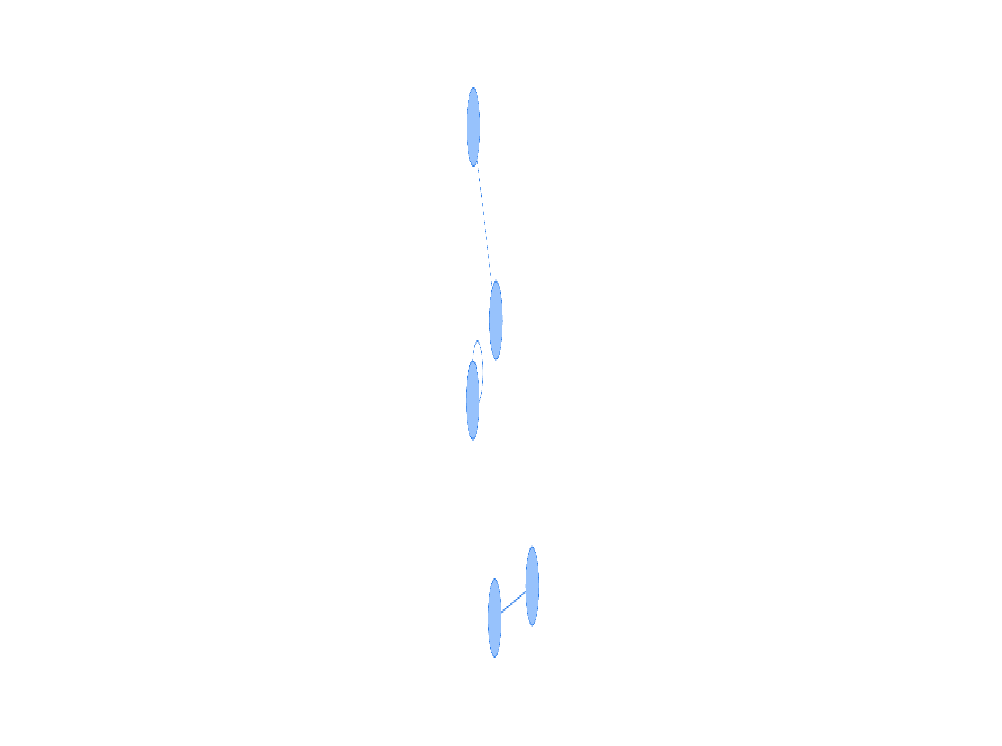
\includegraphics[keepaspectratio]{08-Visnetworks_files/figure-pdf/unnamed-chunk-4-1.pdf}}

En este ejemplo, hemos creado una red con 5 nodos y 3 conexiones entre
ellos. La función \texttt{visNetwork()} toma los data frames de nodos y
enlaces como argumentos y genera una visualización interactiva de la
red. Puedes personalizar la apariencia de los nodos y enlaces utilizando
diferentes atributos, como colores, tamaños, etiquetas, etc.

\subsection{\texorpdfstring{Cómo obtener ayuda en
\texttt{visNetwork}}{Cómo obtener ayuda en visNetwork}}\label{cuxf3mo-obtener-ayuda-en-visnetwork}

Si necesitas ayuda con la función \texttt{visNetwork} o cualquier otra
función de la librería, puedes usar la función \texttt{help()} o el
signo de interrogación \texttt{?} seguido del nombre de la función.
Además, existe ayuda adicional en esta librería usando:

\subsection{Personalización de la
visualización}\label{personalizaciuxf3n-de-la-visualizaciuxf3n}

Puedes personalizar la apariencia de los nodos y enlaces utilizando
diferentes atributos. Por ejemplo, puedes asignar colores a los nodos
según un grupo o categoría, o ajustar el tamaño de los nodos en función
de su grado (número de conexiones).

\begin{Shaded}
\begin{Highlighting}[]
\CommentTok{\# Crear un data frame de nodos con atributos adicionales }
\NormalTok{nodes }\OtherTok{\textless{}{-}} \FunctionTok{data.frame}\NormalTok{(}\AttributeTok{id =} \DecValTok{1}\SpecialCharTok{:}\DecValTok{5}\NormalTok{, }
                    \AttributeTok{label =} \FunctionTok{c}\NormalTok{(}\StringTok{"A"}\NormalTok{, }\StringTok{"B"}\NormalTok{, }\StringTok{"C"}\NormalTok{, }\StringTok{"D"}\NormalTok{, }\StringTok{"E"}\NormalTok{), }
                    \AttributeTok{group =} \FunctionTok{c}\NormalTok{(}\StringTok{"X"}\NormalTok{, }\StringTok{"X"}\NormalTok{, }\StringTok{"Y"}\NormalTok{, }\StringTok{"Y"}\NormalTok{, }\StringTok{"Z"}\NormalTok{),}
                    \AttributeTok{value =} \FunctionTok{c}\NormalTok{(}\DecValTok{10}\NormalTok{, }\DecValTok{20}\NormalTok{, }\DecValTok{30}\NormalTok{, }\DecValTok{40}\NormalTok{, }\DecValTok{50}\NormalTok{))}
\CommentTok{\# Crear un data frame de conexiones}
\NormalTok{edges }\OtherTok{\textless{}{-}} \FunctionTok{data.frame}\NormalTok{(}\AttributeTok{from =} \FunctionTok{c}\NormalTok{(}\DecValTok{1}\NormalTok{,}\DecValTok{2}\NormalTok{,}\DecValTok{5}\NormalTok{), }\AttributeTok{to =} \FunctionTok{c}\NormalTok{(}\DecValTok{3}\NormalTok{,}\DecValTok{4}\NormalTok{,}\DecValTok{5}\NormalTok{))}
\CommentTok{\# Visualizar la red con personalización}
\FunctionTok{visNetwork}\NormalTok{(nodes, edges, }\AttributeTok{width =} \StringTok{"100\%"}\NormalTok{) }\SpecialCharTok{\%\textgreater{}\%}  
  \FunctionTok{visNodes}\NormalTok{(}\AttributeTok{color =} \FunctionTok{list}\NormalTok{(}\AttributeTok{background =} \StringTok{"lightblue"}\NormalTok{, }\AttributeTok{border =} \StringTok{"black"}\NormalTok{)) }\SpecialCharTok{\%\textgreater{}\%}
  \FunctionTok{visEdges}\NormalTok{(}\AttributeTok{color =} \StringTok{"gray"}\NormalTok{) }\SpecialCharTok{\%\textgreater{}\%}
  \FunctionTok{visOptions}\NormalTok{(}\AttributeTok{highlightNearest =} \ConstantTok{TRUE}\NormalTok{, }\AttributeTok{nodesIdSelection =} \ConstantTok{TRUE}\NormalTok{)}
\end{Highlighting}
\end{Shaded}

\pandocbounded{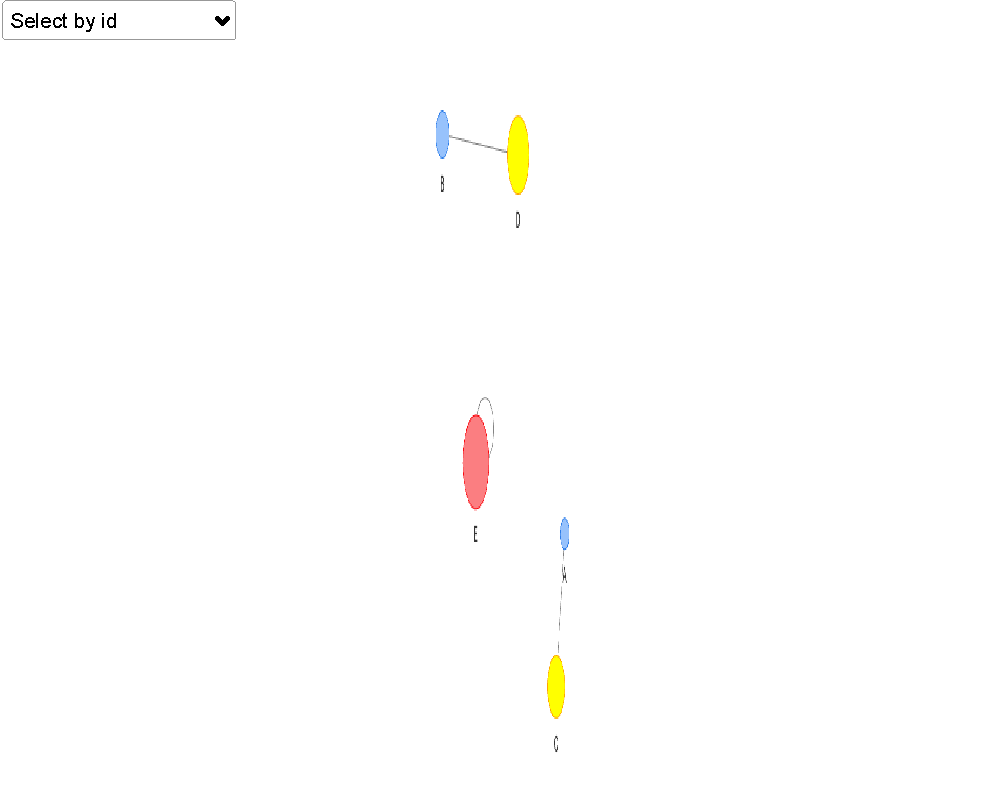
\includegraphics[keepaspectratio]{08-Visnetworks_files/figure-pdf/unnamed-chunk-6-1.pdf}}

En este ejemplo, hemos asignado etiquetas a los nodos, agrupado los
nodos en categorías (X, Y, Z) y asignado un valor que podría representar
el grado o cualquier otra métrica. Además, hemos personalizado los
colores de los nodos y enlaces, y habilitado opciones interactivas como
resaltar el nodo más cercano al pasar el mouse y permitir la selección
de nodos por su ID.

\bookmarksetup{startatroot}

\chapter{Ejercicios integradores}\label{sec-ejercicios-integradores}

\begin{tcolorbox}[enhanced jigsaw, colback=white, toprule=.15mm, title=\textcolor{quarto-callout-note-color}{\faInfo}\hspace{0.5em}{🎯 Propósito de este capítulo}, titlerule=0mm, colframe=quarto-callout-note-color-frame, breakable, opacitybacktitle=0.6, toptitle=1mm, left=2mm, bottomrule=.15mm, bottomtitle=1mm, arc=.35mm, rightrule=.15mm, leftrule=.75mm, opacityback=0, coltitle=black, colbacktitle=quarto-callout-note-color!10!white]

Estos ejercicios combinan conceptos de \textbf{todos los capítulos
anteriores}. Cada uno requiere que apliques múltiples herramientas:
creación de redes, métricas de grado, distancias, clustering y robustez.
Están diseñados para que los resuelvas de forma autónoma, simulando un
análisis de redes completo.

\end{tcolorbox}

\section*{Guía de dificultad}\label{guuxeda-de-dificultad}
\addcontentsline{toc}{section}{Guía de dificultad}

\markright{Guía de dificultad}

\begin{longtable}[]{@{}clc@{}}
\toprule\noalign{}
Nivel & Descripción & Tiempo estimado \\
\midrule\noalign{}
\endhead
\bottomrule\noalign{}
\endlastfoot
⭐ & Aplica funciones directamente & 15--20 min \\
⭐⭐ & Requiere combinar 2--3 conceptos & 30--45 min \\
⭐⭐⭐ & Diseño experimental y análisis completo & 60--90 min \\
\end{longtable}

\section{Preparación del entorno}\label{preparaciuxf3n-del-entorno-7}

\begin{Shaded}
\begin{Highlighting}[]
\FunctionTok{library}\NormalTok{(igraph)}
\FunctionTok{library}\NormalTok{(poweRlaw)}
\end{Highlighting}
\end{Shaded}

\begin{center}\rule{0.5\linewidth}{0.5pt}\end{center}

\section*{Ejercicio integrador 1: Perfil completo de una red
⭐⭐}\label{ejercicio-integrador-1-perfil-completo-de-una-red}
\addcontentsline{toc}{section}{Ejercicio integrador 1: Perfil completo
de una red ⭐⭐}

\markright{Ejercicio integrador 1: Perfil completo de una red ⭐⭐}

Crea una función \texttt{perfil\_red()} que reciba un grafo \texttt{g} y
devuelva un \emph{data frame} con todas las métricas que hemos
aprendido:

\begin{itemize}
\tightlist
\item
  Número de nodos y aristas
\item
  Grado medio, mínimo y máximo
\item
  Densidad de aristas
\item
  Distancia media y diámetro
\item
  Clustering global y promedio
\item
  Número de componentes conectados
\item
  Tamaño del componente gigante (fracción)
\end{itemize}

Prueba tu función con las siguientes cinco redes (todas de 200 nodos):

\begin{enumerate}
\def\labelenumi{\arabic{enumi}.}
\tightlist
\item
  Erdős--Rényi con \(p = 0.03\)
\item
  Barabási--Albert con \(m = 2\)
\item
  \emph{Small-world} con \texttt{nei\ =\ 3}, \(p = 0.05\)
\item
  Anillo
\item
  Estrella
\end{enumerate}

Presenta los resultados en una tabla comparativa y responde: ¿cuál red
tiene la mejor combinación de distancia corta y clustering alto?

\begin{tcolorbox}[enhanced jigsaw, colback=white, toprule=.15mm, title=\textcolor{quarto-callout-tip-color}{\faLightbulb}\hspace{0.5em}{📝 Solución}, titlerule=0mm, colframe=quarto-callout-tip-color-frame, breakable, opacitybacktitle=0.6, toptitle=1mm, left=2mm, bottomrule=.15mm, bottomtitle=1mm, arc=.35mm, rightrule=.15mm, leftrule=.75mm, opacityback=0, coltitle=black, colbacktitle=quarto-callout-tip-color!10!white]

\textbf{Paso 1:} Definir la función.

\begin{Shaded}
\begin{Highlighting}[]
\NormalTok{perfil\_red }\OtherTok{\textless{}{-}} \ControlFlowTok{function}\NormalTok{(g) \{}
\NormalTok{  comp }\OtherTok{\textless{}{-}} \FunctionTok{components}\NormalTok{(g)}
  
  \CommentTok{\# Eficiencia: promedio de 1/d(i,j)}
\NormalTok{  d }\OtherTok{\textless{}{-}} \FunctionTok{distances}\NormalTok{(g)}
\NormalTok{  n }\OtherTok{\textless{}{-}} \FunctionTok{vcount}\NormalTok{(g)}
\NormalTok{  inv\_d }\OtherTok{\textless{}{-}} \FunctionTok{ifelse}\NormalTok{(d }\SpecialCharTok{==} \DecValTok{0} \SpecialCharTok{|} \FunctionTok{is.infinite}\NormalTok{(d), }\DecValTok{0}\NormalTok{, }\DecValTok{1} \SpecialCharTok{/}\NormalTok{ d)}
\NormalTok{  eficiencia }\OtherTok{\textless{}{-}} \FunctionTok{sum}\NormalTok{(inv\_d) }\SpecialCharTok{/}\NormalTok{ (n }\SpecialCharTok{*}\NormalTok{ (n }\SpecialCharTok{{-}} \DecValTok{1}\NormalTok{))}
  
  \FunctionTok{data.frame}\NormalTok{(}
    \AttributeTok{Nodos            =} \FunctionTok{vcount}\NormalTok{(g),}
    \AttributeTok{Aristas          =} \FunctionTok{ecount}\NormalTok{(g),}
    \AttributeTok{Grado\_medio      =} \FunctionTok{round}\NormalTok{(}\FunctionTok{mean}\NormalTok{(}\FunctionTok{degree}\NormalTok{(g)), }\DecValTok{2}\NormalTok{),}
    \AttributeTok{Grado\_min        =} \FunctionTok{min}\NormalTok{(}\FunctionTok{degree}\NormalTok{(g)),}
    \AttributeTok{Grado\_max        =} \FunctionTok{max}\NormalTok{(}\FunctionTok{degree}\NormalTok{(g)),}
    \AttributeTok{Densidad         =} \FunctionTok{round}\NormalTok{(}\FunctionTok{edge\_density}\NormalTok{(g), }\DecValTok{4}\NormalTok{),}
    \AttributeTok{Dist\_media       =} \FunctionTok{round}\NormalTok{(}\FunctionTok{mean\_distance}\NormalTok{(g), }\DecValTok{3}\NormalTok{),}
\NormalTok{    Diámetro         }\OtherTok{=} \FunctionTok{diameter}\NormalTok{(g),}
    \AttributeTok{C\_global         =} \FunctionTok{round}\NormalTok{(}\FunctionTok{transitivity}\NormalTok{(g, }\AttributeTok{type =} \StringTok{"global"}\NormalTok{), }\DecValTok{4}\NormalTok{),}
    \AttributeTok{C\_promedio       =} \FunctionTok{round}\NormalTok{(}\FunctionTok{transitivity}\NormalTok{(g, }\AttributeTok{type =} \StringTok{"average"}\NormalTok{), }\DecValTok{4}\NormalTok{),}
    \AttributeTok{Componentes      =}\NormalTok{ comp}\SpecialCharTok{$}\NormalTok{no,}
    \AttributeTok{Comp\_gigante\_pct =} \FunctionTok{round}\NormalTok{(}\FunctionTok{max}\NormalTok{(comp}\SpecialCharTok{$}\NormalTok{csize) }\SpecialCharTok{/} \FunctionTok{vcount}\NormalTok{(g) }\SpecialCharTok{*} \DecValTok{100}\NormalTok{, }\DecValTok{1}\NormalTok{),}
    \AttributeTok{Eficiencia       =} \FunctionTok{round}\NormalTok{(eficiencia, }\DecValTok{4}\NormalTok{)}
\NormalTok{  )}
\NormalTok{\}}
\end{Highlighting}
\end{Shaded}

\textbf{Paso 2:} Generar las redes y calcular perfiles.

\begin{Shaded}
\begin{Highlighting}[]
\FunctionTok{set.seed}\NormalTok{(}\DecValTok{42}\NormalTok{)}

\NormalTok{redes\_perfil }\OtherTok{\textless{}{-}} \FunctionTok{list}\NormalTok{(}
  \StringTok{"Erdős–Rényi"}     \OtherTok{=} \FunctionTok{sample\_gnp}\NormalTok{(}\DecValTok{200}\NormalTok{, }\FloatTok{0.03}\NormalTok{),}
  \StringTok{"Barabási–Albert"}  \OtherTok{=} \FunctionTok{sample\_pa}\NormalTok{(}\DecValTok{200}\NormalTok{, }\AttributeTok{m =} \DecValTok{2}\NormalTok{, }\AttributeTok{directed =} \ConstantTok{FALSE}\NormalTok{),}
  \StringTok{"Small{-}world"}      \OtherTok{=} \FunctionTok{sample\_smallworld}\NormalTok{(}\DecValTok{1}\NormalTok{, }\DecValTok{200}\NormalTok{, }\AttributeTok{nei =} \DecValTok{3}\NormalTok{, }\AttributeTok{p =} \FloatTok{0.05}\NormalTok{),}
  \StringTok{"Anillo"}           \OtherTok{=} \FunctionTok{make\_ring}\NormalTok{(}\DecValTok{200}\NormalTok{),}
  \StringTok{"Estrella"}         \OtherTok{=} \FunctionTok{make\_star}\NormalTok{(}\DecValTok{200}\NormalTok{, }\AttributeTok{mode =} \StringTok{"undirected"}\NormalTok{)}
\NormalTok{)}

\CommentTok{\# Calcular el perfil de cada red}
\NormalTok{perfiles }\OtherTok{\textless{}{-}} \FunctionTok{do.call}\NormalTok{(rbind, }\FunctionTok{lapply}\NormalTok{(redes\_perfil, perfil\_red))}
\NormalTok{perfiles }\OtherTok{\textless{}{-}} \FunctionTok{cbind}\NormalTok{(}\AttributeTok{Red =} \FunctionTok{names}\NormalTok{(redes\_perfil), perfiles)}
\FunctionTok{rownames}\NormalTok{(perfiles) }\OtherTok{\textless{}{-}} \ConstantTok{NULL}

\NormalTok{knitr}\SpecialCharTok{::}\FunctionTok{kable}\NormalTok{(perfiles,}
             \AttributeTok{caption =} \StringTok{"Perfil completo de cinco topologías con 200 nodos"}\NormalTok{)}
\end{Highlighting}
\end{Shaded}

\begin{longtable}[]{@{}
  >{\raggedright\arraybackslash}p{(\linewidth - 26\tabcolsep) * \real{0.1060}}
  >{\raggedleft\arraybackslash}p{(\linewidth - 26\tabcolsep) * \real{0.0397}}
  >{\raggedleft\arraybackslash}p{(\linewidth - 26\tabcolsep) * \real{0.0530}}
  >{\raggedleft\arraybackslash}p{(\linewidth - 26\tabcolsep) * \real{0.0795}}
  >{\raggedleft\arraybackslash}p{(\linewidth - 26\tabcolsep) * \real{0.0662}}
  >{\raggedleft\arraybackslash}p{(\linewidth - 26\tabcolsep) * \real{0.0662}}
  >{\raggedleft\arraybackslash}p{(\linewidth - 26\tabcolsep) * \real{0.0596}}
  >{\raggedleft\arraybackslash}p{(\linewidth - 26\tabcolsep) * \real{0.0728}}
  >{\raggedleft\arraybackslash}p{(\linewidth - 26\tabcolsep) * \real{0.0596}}
  >{\raggedleft\arraybackslash}p{(\linewidth - 26\tabcolsep) * \real{0.0596}}
  >{\raggedleft\arraybackslash}p{(\linewidth - 26\tabcolsep) * \real{0.0728}}
  >{\raggedleft\arraybackslash}p{(\linewidth - 26\tabcolsep) * \real{0.0795}}
  >{\raggedleft\arraybackslash}p{(\linewidth - 26\tabcolsep) * \real{0.1126}}
  >{\raggedleft\arraybackslash}p{(\linewidth - 26\tabcolsep) * \real{0.0728}}@{}}
\caption{Perfil completo de cinco topologías con 200
nodos}\tabularnewline
\toprule\noalign{}
\begin{minipage}[b]{\linewidth}\raggedright
Red
\end{minipage} & \begin{minipage}[b]{\linewidth}\raggedleft
Nodos
\end{minipage} & \begin{minipage}[b]{\linewidth}\raggedleft
Aristas
\end{minipage} & \begin{minipage}[b]{\linewidth}\raggedleft
Grado\_medio
\end{minipage} & \begin{minipage}[b]{\linewidth}\raggedleft
Grado\_min
\end{minipage} & \begin{minipage}[b]{\linewidth}\raggedleft
Grado\_max
\end{minipage} & \begin{minipage}[b]{\linewidth}\raggedleft
Densidad
\end{minipage} & \begin{minipage}[b]{\linewidth}\raggedleft
Dist\_media
\end{minipage} & \begin{minipage}[b]{\linewidth}\raggedleft
Diámetro
\end{minipage} & \begin{minipage}[b]{\linewidth}\raggedleft
C\_global
\end{minipage} & \begin{minipage}[b]{\linewidth}\raggedleft
C\_promedio
\end{minipage} & \begin{minipage}[b]{\linewidth}\raggedleft
Componentes
\end{minipage} & \begin{minipage}[b]{\linewidth}\raggedleft
Comp\_gigante\_pct
\end{minipage} & \begin{minipage}[b]{\linewidth}\raggedleft
Eficiencia
\end{minipage} \\
\midrule\noalign{}
\endfirsthead
\toprule\noalign{}
\begin{minipage}[b]{\linewidth}\raggedright
Red
\end{minipage} & \begin{minipage}[b]{\linewidth}\raggedleft
Nodos
\end{minipage} & \begin{minipage}[b]{\linewidth}\raggedleft
Aristas
\end{minipage} & \begin{minipage}[b]{\linewidth}\raggedleft
Grado\_medio
\end{minipage} & \begin{minipage}[b]{\linewidth}\raggedleft
Grado\_min
\end{minipage} & \begin{minipage}[b]{\linewidth}\raggedleft
Grado\_max
\end{minipage} & \begin{minipage}[b]{\linewidth}\raggedleft
Densidad
\end{minipage} & \begin{minipage}[b]{\linewidth}\raggedleft
Dist\_media
\end{minipage} & \begin{minipage}[b]{\linewidth}\raggedleft
Diámetro
\end{minipage} & \begin{minipage}[b]{\linewidth}\raggedleft
C\_global
\end{minipage} & \begin{minipage}[b]{\linewidth}\raggedleft
C\_promedio
\end{minipage} & \begin{minipage}[b]{\linewidth}\raggedleft
Componentes
\end{minipage} & \begin{minipage}[b]{\linewidth}\raggedleft
Comp\_gigante\_pct
\end{minipage} & \begin{minipage}[b]{\linewidth}\raggedleft
Eficiencia
\end{minipage} \\
\midrule\noalign{}
\endhead
\bottomrule\noalign{}
\endlastfoot
Erdős--Rényi & 200 & 578 & 5.78 & 0 & 14 & 0.0290 & 3.181 & 6 & 0.0267 &
0.0270 & 2 & 99.5 & 0.3436 \\
Barabási--Albert & 200 & 397 & 3.97 & 2 & 28 & 0.0199 & 3.586 & 6 &
0.0292 & 0.0491 & 1 & 100.0 & 0.3086 \\
Small-world & 200 & 600 & 6.00 & 3 & 9 & 0.0302 & 4.253 & 7 & 0.4150 &
0.4329 & 1 & 100.0 & 0.2734 \\
Anillo & 200 & 200 & 2.00 & 2 & 2 & 0.0101 & 50.251 & 100 & 0.0000 &
0.0000 & 1 & 100.0 & 0.0521 \\
Estrella & 200 & 199 & 1.99 & 1 & 199 & 0.0100 & 1.990 & 2 & 0.0000 &
0.0000 & 1 & 100.0 & 0.5050 \\
\end{longtable}

\textbf{Interpretación:} La red \emph{small-world} ofrece la mejor
combinación de distancia corta y clustering alto. La estrella tiene la
menor distancia media pero clustering cero. La red completa sería ideal
en ambas métricas, pero requiere \(\binom{200}{2} = 19{,}900\) aristas,
mientras que la \emph{small-world} logra un excelente balance con solo
\textasciitilde600.

\end{tcolorbox}

\begin{center}\rule{0.5\linewidth}{0.5pt}\end{center}

\section*{Ejercicio integrador 2: Red social de una clase
⭐⭐}\label{ejercicio-integrador-2-red-social-de-una-clase}
\addcontentsline{toc}{section}{Ejercicio integrador 2: Red social de una
clase ⭐⭐}

\markright{Ejercicio integrador 2: Red social de una clase ⭐⭐}

Diseña una red que represente las relaciones de colaboración en un grupo
de 20 estudiantes. Las reglas son:

\begin{enumerate}
\def\labelenumi{\arabic{enumi}.}
\tightlist
\item
  Cada estudiante tiene un nombre (invéntalos o usa
  \texttt{paste0("Est\_",\ 1:20)}).
\item
  Cada estudiante pertenece a uno de 4 equipos de proyecto (5 por
  equipo).
\item
  Dentro de cada equipo, todos están conectados entre sí (clique).
\item
  Entre equipos, agrega 8 conexiones aleatorias (simulando amistades
  inter-equipo).
\end{enumerate}

Con la red construida:

\begin{enumerate}
\def\labelenumi{\alph{enumi})}
\tightlist
\item
  Visualiza la red coloreando por equipo.
\item
  Calcula el clustering local de cada nodo. ¿Los nodos ``puente'' (con
  conexiones inter-equipo) tienen clustering diferente?
\item
  Encuentra el nodo con mayor \emph{betweenness centrality}. ¿Es un
  puente?
\item
  Simula la eliminación de ese nodo. ¿Cómo cambian la distancia media y
  el número de componentes?
\end{enumerate}

\begin{tcolorbox}[enhanced jigsaw, colback=white, toprule=.15mm, title=\textcolor{quarto-callout-note-color}{\faInfo}\hspace{0.5em}{💡 Pista 1}, titlerule=0mm, colframe=quarto-callout-note-color-frame, breakable, opacitybacktitle=0.6, toptitle=1mm, left=2mm, bottomrule=.15mm, bottomtitle=1mm, arc=.35mm, rightrule=.15mm, leftrule=.75mm, opacityback=0, coltitle=black, colbacktitle=quarto-callout-note-color!10!white]

Para crear los cliques por equipo, usa \texttt{make\_full\_graph(5)}
cuatro veces y luego \texttt{disjoint\_union()} para combinarlos.
Después agrega las aristas inter-equipo con \texttt{add\_edges()}.

\end{tcolorbox}

\begin{tcolorbox}[enhanced jigsaw, colback=white, toprule=.15mm, title=\textcolor{quarto-callout-note-color}{\faInfo}\hspace{0.5em}{💡 Pista 2}, titlerule=0mm, colframe=quarto-callout-note-color-frame, breakable, opacitybacktitle=0.6, toptitle=1mm, left=2mm, bottomrule=.15mm, bottomtitle=1mm, arc=.35mm, rightrule=.15mm, leftrule=.75mm, opacityback=0, coltitle=black, colbacktitle=quarto-callout-note-color!10!white]

Los colores por equipo se asignan fácilmente:
\texttt{V(g)\$color\ \textless{}-\ rep(c("tomato",\ "skyblue",\ "gold",\ "lightgreen"),\ each\ =\ 5)}.
La \emph{betweenness centrality} se calcula con \texttt{betweenness(g)}.

\end{tcolorbox}

\begin{tcolorbox}[enhanced jigsaw, colback=white, toprule=.15mm, title=\textcolor{quarto-callout-note-color}{\faInfo}\hspace{0.5em}{💡 Pista 3 --- Pseudocódigo}, titlerule=0mm, colframe=quarto-callout-note-color-frame, breakable, opacitybacktitle=0.6, toptitle=1mm, left=2mm, bottomrule=.15mm, bottomtitle=1mm, arc=.35mm, rightrule=.15mm, leftrule=.75mm, opacityback=0, coltitle=black, colbacktitle=quarto-callout-note-color!10!white]

\begin{verbatim}
1. set.seed(42)
2. # Crear 4 cliques
3. equipos <- disjoint_union(make_full_graph(5), make_full_graph(5),
4.                           make_full_graph(5), make_full_graph(5))
5. V(equipos)$name <- paste0("Est_", 1:20)
6. V(equipos)$equipo <- rep(1:4, each = 5)
7. V(equipos)$color <- rep(c("tomato","skyblue","gold","lightgreen"), each=5)
8. 
9. # Agregar 8 conexiones inter-equipo aleatorias
10. for (k in 1:8) {
11.   e1 <- sample(1:5, 1) + (sample(0:3, 1) * 5)
12.   e2 <- sample(1:5, 1) + (sample(0:3, 1) * 5)
13.   while (V(equipos)$equipo[e1] == V(equipos)$equipo[e2]) {
14.     e2 <- sample(1:5, 1) + (sample(0:3, 1) * 5)
15.   }
16.   equipos <- add_edges(equipos, c(e1, e2))
17. }
18. 
19. plot(equipos)
20. betweenness(equipos)
21. transitivity(equipos, type = "local")
\end{verbatim}

\end{tcolorbox}

\begin{center}\rule{0.5\linewidth}{0.5pt}\end{center}

\section*{Ejercicio integrador 3: Epidemia en tres topologías
⭐⭐⭐}\label{ejercicio-integrador-3-epidemia-en-tres-topologuxedas}
\addcontentsline{toc}{section}{Ejercicio integrador 3: Epidemia en tres
topologías ⭐⭐⭐}

\markright{Ejercicio integrador 3: Epidemia en tres topologías ⭐⭐⭐}

Simula una epidemia SIR (\emph{Susceptible → Infectado → Recuperado})
simplificada en tres tipos de red con 500 nodos: ER (\(p = 0.01\)), BA
(\(m = 2\)) y \emph{small-world} (\texttt{nei\ =\ 3}, \(p = 0.1\)).

\textbf{Reglas de la epidemia (por ronda):}

\begin{enumerate}
\def\labelenumi{\arabic{enumi}.}
\tightlist
\item
  Comienza con 1 nodo infectado al azar.
\item
  Cada nodo infectado contagia a cada vecino susceptible con
  probabilidad \(\beta = 0.3\).
\item
  Cada nodo infectado se recupera (y se vuelve inmune) con probabilidad
  \(\gamma = 0.1\).
\item
  La epidemia termina cuando no quedan infectados.
\end{enumerate}

\textbf{Tareas:}

\begin{enumerate}
\def\labelenumi{\alph{enumi})}
\tightlist
\item
  Implementa la simulación como una función
  \texttt{simular\_sir(g,\ beta,\ gamma,\ semilla)}.
\item
  Ejecuta 20 realizaciones por red. Registra el número final de
  recuperados (= total de infectados acumulados).
\item
  Presenta boxplots del total de infectados por tipo de red.
\item
  ¿En qué red se propaga más rápido la epidemia? ¿En cuál infecta a más
  personas en total?
\item
  Relaciona los resultados con las métricas de distancia y clustering de
  cada red.
\end{enumerate}

\begin{tcolorbox}[enhanced jigsaw, colback=white, toprule=.15mm, title=\textcolor{quarto-callout-note-color}{\faInfo}\hspace{0.5em}{💡 Pista 1}, titlerule=0mm, colframe=quarto-callout-note-color-frame, breakable, opacitybacktitle=0.6, toptitle=1mm, left=2mm, bottomrule=.15mm, bottomtitle=1mm, arc=.35mm, rightrule=.15mm, leftrule=.75mm, opacityback=0, coltitle=black, colbacktitle=quarto-callout-note-color!10!white]

Usa tres vectores de estado: \texttt{S}, \texttt{I}, \texttt{R} (lógicos
o numéricos). En cada ronda, para cada infectado, recorre sus vecinos
con \texttt{neighbors(g,\ v)} y contagia con
\texttt{rbinom(1,\ 1,\ beta)}.

\end{tcolorbox}

\begin{tcolorbox}[enhanced jigsaw, colback=white, toprule=.15mm, title=\textcolor{quarto-callout-note-color}{\faInfo}\hspace{0.5em}{💡 Pista 2}, titlerule=0mm, colframe=quarto-callout-note-color-frame, breakable, opacitybacktitle=0.6, toptitle=1mm, left=2mm, bottomrule=.15mm, bottomtitle=1mm, arc=.35mm, rightrule=.15mm, leftrule=.75mm, opacityback=0, coltitle=black, colbacktitle=quarto-callout-note-color!10!white]

Estructura de la función:

\begin{Shaded}
\begin{Highlighting}[]
\NormalTok{simular\_sir }\OtherTok{\textless{}{-}} \ControlFlowTok{function}\NormalTok{(g, }\AttributeTok{beta =} \FloatTok{0.3}\NormalTok{, }\AttributeTok{gamma =} \FloatTok{0.1}\NormalTok{, }\AttributeTok{semilla =} \DecValTok{42}\NormalTok{) \{}
  \FunctionTok{set.seed}\NormalTok{(semilla)}
\NormalTok{  n }\OtherTok{\textless{}{-}} \FunctionTok{vcount}\NormalTok{(g)}
\NormalTok{  estado }\OtherTok{\textless{}{-}} \FunctionTok{rep}\NormalTok{(}\StringTok{"S"}\NormalTok{, n)  }\CommentTok{\# S, I, R}
\NormalTok{  paciente\_cero }\OtherTok{\textless{}{-}} \FunctionTok{sample}\NormalTok{(}\DecValTok{1}\SpecialCharTok{:}\NormalTok{n, }\DecValTok{1}\NormalTok{)}
\NormalTok{  estado[paciente\_cero] }\OtherTok{\textless{}{-}} \StringTok{"I"}
\NormalTok{  historial }\OtherTok{\textless{}{-}} \FunctionTok{data.frame}\NormalTok{(}\AttributeTok{ronda =} \DecValTok{0}\NormalTok{, }\AttributeTok{S =}\NormalTok{ n}\DecValTok{{-}1}\NormalTok{, }\AttributeTok{I =} \DecValTok{1}\NormalTok{, }\AttributeTok{R =} \DecValTok{0}\NormalTok{)}
  
  \ControlFlowTok{while}\NormalTok{ (}\FunctionTok{sum}\NormalTok{(estado }\SpecialCharTok{==} \StringTok{"I"}\NormalTok{) }\SpecialCharTok{\textgreater{}} \DecValTok{0}\NormalTok{) \{}
    \CommentTok{\# ... contagio y recuperación ...}
\NormalTok{  \}}
\NormalTok{  historial}
\NormalTok{\}}
\end{Highlighting}
\end{Shaded}

\end{tcolorbox}

\begin{tcolorbox}[enhanced jigsaw, colback=white, toprule=.15mm, title=\textcolor{quarto-callout-note-color}{\faInfo}\hspace{0.5em}{💡 Pista 3 --- Pseudocódigo}, titlerule=0mm, colframe=quarto-callout-note-color-frame, breakable, opacitybacktitle=0.6, toptitle=1mm, left=2mm, bottomrule=.15mm, bottomtitle=1mm, arc=.35mm, rightrule=.15mm, leftrule=.75mm, opacityback=0, coltitle=black, colbacktitle=quarto-callout-note-color!10!white]

\begin{verbatim}
Para cada ronda mientras haya infectados:
  1. nuevos_infectados <- c()
  2. Para cada nodo infectado v:
     a) Para cada vecino u de v:
        - Si u es susceptible y runif(1) < beta:
          nuevos_infectados <- c(nuevos_infectados, u)
     b) Si runif(1) < gamma: estado[v] <- "R"
  3. estado[nuevos_infectados] <- "I"
  4. Registrar conteos S, I, R
\end{verbatim}

La red BA debería propagar más rápido (distancia corta, hubs actúan como
super-propagadores). La \emph{small-world} debería alcanzar más personas
en total (clustering alto = propagación local eficiente + atajos para
propagación global).

\end{tcolorbox}

\begin{center}\rule{0.5\linewidth}{0.5pt}\end{center}

\section*{Ejercicio integrador 4: Análisis de robustez comparativo
completo
⭐⭐⭐}\label{ejercicio-integrador-4-anuxe1lisis-de-robustez-comparativo-completo}
\addcontentsline{toc}{section}{Ejercicio integrador 4: Análisis de
robustez comparativo completo ⭐⭐⭐}

\markright{Ejercicio integrador 4: Análisis de robustez comparativo
completo ⭐⭐⭐}

Realiza un análisis de robustez exhaustivo de tres redes de 300 nodos:
ER (\(p = 0.02\)), BA (\(m = 2\)) y \emph{small-world}
(\texttt{nei\ =\ 3}, \(p = 0.1\)).

\textbf{Tareas:}

\begin{enumerate}
\def\labelenumi{\alph{enumi})}
\item
  Para cada red, ejecuta:

  \begin{itemize}
  \tightlist
  \item
    10 simulaciones de fallos aleatorios (eliminando hasta el 50\% de
    nodos).
  \item
    1 simulación de ataque dirigido por grado (determinista).
  \item
    1 simulación de ataque dirigido por \emph{betweenness}.
  \end{itemize}
\item
  Genera un panel de 6 gráficos (3 redes × 2 escenarios: fallo
  vs.~ataque) mostrando la evolución del componente gigante. Para los
  fallos, incluye la media y la banda de ± 1 DE.
\item
  Calcula el ``índice de robustez'' \(R\) (área bajo la curva del
  componente gigante) para cada escenario y presenta una tabla resumen.
\item
  Redacta un párrafo de conclusiones comparando las tres topologías.
\end{enumerate}

\begin{tcolorbox}[enhanced jigsaw, colback=white, toprule=.15mm, title=\textcolor{quarto-callout-note-color}{\faInfo}\hspace{0.5em}{💡 Pista 1}, titlerule=0mm, colframe=quarto-callout-note-color-frame, breakable, opacitybacktitle=0.6, toptitle=1mm, left=2mm, bottomrule=.15mm, bottomtitle=1mm, arc=.35mm, rightrule=.15mm, leftrule=.75mm, opacityback=0, coltitle=black, colbacktitle=quarto-callout-note-color!10!white]

El índice \(R\) se calcula como el área bajo la curva del componente
gigante vs.~fracción eliminada. Usa la regla del trapecio:

\begin{Shaded}
\begin{Highlighting}[]
\NormalTok{indice\_R }\OtherTok{\textless{}{-}} \ControlFlowTok{function}\NormalTok{(x, y) \{}
  \FunctionTok{sum}\NormalTok{(}\FunctionTok{diff}\NormalTok{(x) }\SpecialCharTok{*}\NormalTok{ (y[}\SpecialCharTok{{-}}\FunctionTok{length}\NormalTok{(y)] }\SpecialCharTok{+}\NormalTok{ y[}\SpecialCharTok{{-}}\DecValTok{1}\NormalTok{]) }\SpecialCharTok{/} \DecValTok{2}\NormalTok{)}
\NormalTok{\}}
\end{Highlighting}
\end{Shaded}

Un \(R = 0.5\) corresponde a una degradación lineal; \(R > 0.5\) indica
robustez; \(R < 0.5\) indica fragilidad.

\end{tcolorbox}

\begin{tcolorbox}[enhanced jigsaw, colback=white, toprule=.15mm, title=\textcolor{quarto-callout-note-color}{\faInfo}\hspace{0.5em}{💡 Pista 2}, titlerule=0mm, colframe=quarto-callout-note-color-frame, breakable, opacitybacktitle=0.6, toptitle=1mm, left=2mm, bottomrule=.15mm, bottomtitle=1mm, arc=.35mm, rightrule=.15mm, leftrule=.75mm, opacityback=0, coltitle=black, colbacktitle=quarto-callout-note-color!10!white]

Para el panel de 6 gráficos, usa \texttt{par(mfrow\ =\ c(2,\ 3))}. Fila
superior: fallos aleatorios. Fila inferior: ataques. Columnas: ER, BA,
SW.

\end{tcolorbox}

\begin{center}\rule{0.5\linewidth}{0.5pt}\end{center}

\section*{Ejercicio integrador 5: Red de ingredientes
⭐⭐}\label{ejercicio-integrador-5-red-de-ingredientes}
\addcontentsline{toc}{section}{Ejercicio integrador 5: Red de
ingredientes ⭐⭐}

\markright{Ejercicio integrador 5: Red de ingredientes ⭐⭐}

Diseña una red donde los nodos representen 15 ingredientes de cocina
mexicana y las aristas indiquen que dos ingredientes aparecen juntos en
al menos una receta.

\textbf{Ingredientes sugeridos:} chile, tomate, cebolla, ajo, cilantro,
limón, aguacate, frijol, maíz, queso, crema, pollo, arroz, tortilla,
sal.

\textbf{Tareas:}

\begin{enumerate}
\def\labelenumi{\alph{enumi})}
\tightlist
\item
  Define las conexiones manualmente con \texttt{graph\_from\_literal()}
  basándote en recetas reales (salsa mexicana, guacamole, tacos,
  enchiladas, arroz rojo, etc.).
\item
  Visualiza la red con tamaño de nodo proporcional al grado.
\item
  ¿Cuál es el ingrediente más ``central'' (mayor grado)? ¿Coincide con
  tu intuición culinaria?
\item
  Calcula la distancia media. ¿Los ingredientes están ``cerca'' unos de
  otros?
\item
  Identifica si hay comunidades usando \texttt{cluster\_louvain()} o
  \texttt{cluster\_walktrap()}. ¿Las comunidades corresponden a tipos de
  ingrediente (proteínas, vegetales, condimentos)?
\item
  Elimina el ingrediente más conectado. ¿Cómo cambia la estructura de la
  red?
\end{enumerate}

\begin{tcolorbox}[enhanced jigsaw, colback=white, toprule=.15mm, title=\textcolor{quarto-callout-note-color}{\faInfo}\hspace{0.5em}{💡 Pista 1}, titlerule=0mm, colframe=quarto-callout-note-color-frame, breakable, opacitybacktitle=0.6, toptitle=1mm, left=2mm, bottomrule=.15mm, bottomtitle=1mm, arc=.35mm, rightrule=.15mm, leftrule=.75mm, opacityback=0, coltitle=black, colbacktitle=quarto-callout-note-color!10!white]

Un ejemplo de definición:

\begin{Shaded}
\begin{Highlighting}[]
\NormalTok{g }\OtherTok{\textless{}{-}} \FunctionTok{graph\_from\_literal}\NormalTok{(}
\NormalTok{  chile }\SpecialCharTok{{-}{-}}\NormalTok{ tomate, chile }\SpecialCharTok{{-}{-}}\NormalTok{ cebolla, chile }\SpecialCharTok{{-}{-}}\NormalTok{ ajo,}
\NormalTok{  tomate }\SpecialCharTok{{-}{-}}\NormalTok{ cebolla, tomate }\SpecialCharTok{{-}{-}}\NormalTok{ cilantro, tomate }\SpecialCharTok{{-}{-}}\NormalTok{ limón,}
\NormalTok{  aguacate }\SpecialCharTok{{-}{-}}\NormalTok{ limón, aguacate }\SpecialCharTok{{-}{-}}\NormalTok{ cilantro, aguacate }\SpecialCharTok{{-}{-}}\NormalTok{ tomate, aguacate }\SpecialCharTok{{-}{-}}\NormalTok{ sal,}
  \CommentTok{\# ... continuar con más recetas}
\NormalTok{)}
\end{Highlighting}
\end{Shaded}

\end{tcolorbox}

\begin{tcolorbox}[enhanced jigsaw, colback=white, toprule=.15mm, title=\textcolor{quarto-callout-note-color}{\faInfo}\hspace{0.5em}{💡 Pista 2}, titlerule=0mm, colframe=quarto-callout-note-color-frame, breakable, opacitybacktitle=0.6, toptitle=1mm, left=2mm, bottomrule=.15mm, bottomtitle=1mm, arc=.35mm, rightrule=.15mm, leftrule=.75mm, opacityback=0, coltitle=black, colbacktitle=quarto-callout-note-color!10!white]

Para detectar comunidades:
\texttt{com\ \textless{}-\ cluster\_walktrap(g)} y luego
\texttt{membership(com)} te da el grupo de cada nodo. Colorea con
\texttt{V(g)\$color\ \textless{}-\ membership(com)}.

\end{tcolorbox}

\begin{center}\rule{0.5\linewidth}{0.5pt}\end{center}

\section*{Ejercicio integrador 6: Construir desde archivo
⭐⭐}\label{ejercicio-integrador-6-construir-desde-archivo}
\addcontentsline{toc}{section}{Ejercicio integrador 6: Construir desde
archivo ⭐⭐}

\markright{Ejercicio integrador 6: Construir desde archivo ⭐⭐}

Crea dos archivos CSV: uno de nodos y otro de aristas para representar
una red de colaboración entre 12 investigadores.

\textbf{Archivo \texttt{nodos.csv}:}

\begin{longtable}[]{@{}llll@{}}
\toprule\noalign{}
id & nombre & departamento & publicaciones \\
\midrule\noalign{}
\endhead
\bottomrule\noalign{}
\endlastfoot
1 & Ana & Biología & 15 \\
2 & Beto & Física & 22 \\
\ldots{} & \ldots{} & \ldots{} & \ldots{} \\
\end{longtable}

\textbf{Archivo \texttt{aristas.csv}:}

\begin{longtable}[]{@{}lll@{}}
\toprule\noalign{}
from & to & peso \\
\midrule\noalign{}
\endhead
\bottomrule\noalign{}
\endlastfoot
1 & 2 & 3 \\
1 & 5 & 1 \\
\ldots{} & \ldots{} & \ldots{} \\
\end{longtable}

\textbf{Tareas:}

\begin{enumerate}
\def\labelenumi{\alph{enumi})}
\tightlist
\item
  Crea ambos archivos con \texttt{write.csv()} y léelos con
  \texttt{read.csv()}.
\item
  Construye la red con
  \texttt{graph\_from\_data\_frame(d\ =\ aristas,\ vertices\ =\ nodos,\ directed\ =\ FALSE)}.
\item
  Limpia la red con \texttt{simplify()}.
\item
  Visualiza con tamaño proporcional a publicaciones y color por
  departamento.
\item
  Calcula el perfil completo (usa \texttt{perfil\_red()} del Ejercicio 1
  si lo resolviste).
\item
  ¿Quién es el investigador más central por \emph{betweenness}? ¿Conecta
  departamentos diferentes?
\end{enumerate}

\begin{tcolorbox}[enhanced jigsaw, colback=white, toprule=.15mm, title=\textcolor{quarto-callout-note-color}{\faInfo}\hspace{0.5em}{💡 Pista 1}, titlerule=0mm, colframe=quarto-callout-note-color-frame, breakable, opacitybacktitle=0.6, toptitle=1mm, left=2mm, bottomrule=.15mm, bottomtitle=1mm, arc=.35mm, rightrule=.15mm, leftrule=.75mm, opacityback=0, coltitle=black, colbacktitle=quarto-callout-note-color!10!white]

Diseña la red pensando en que las colaboraciones inter-departamento sean
menos frecuentes que las intra-departamento. Así la detección de
comunidades debería encontrar los departamentos.

\end{tcolorbox}

\begin{center}\rule{0.5\linewidth}{0.5pt}\end{center}

\section*{Ejercicio integrador 7: Power-law en el mundo real
⭐⭐⭐}\label{ejercicio-integrador-7-power-law-en-el-mundo-real}
\addcontentsline{toc}{section}{Ejercicio integrador 7: Power-law en el
mundo real ⭐⭐⭐}

\markright{Ejercicio integrador 7: Power-law en el mundo real ⭐⭐⭐}

Genera una red BA de 5000 nodos con \(m = 2\). Realiza un análisis
completo de su distribución de grado:

\begin{enumerate}
\def\labelenumi{\alph{enumi})}
\tightlist
\item
  Histograma de grado con ejes lineales.
\item
  Histograma con eje y logarítmico.
\item
  Gráfico log-log de la distribución de grado (CCDF).
\item
  Ajuste de ley de potencia con \texttt{poweRlaw}: reporta \(\gamma\) y
  \(x_{\min}\).
\item
  Superpón el ajuste sobre el gráfico CCDF.
\item
  Compara con una red ER del mismo tamaño: ¿el ajuste \emph{power-law}
  tiene sentido para la red ER?
\item
  Identifica los 20 \emph{hubs} principales. ¿Qué fracción de las
  aristas totales concentran?
\item
  Elimina los 20 \emph{hubs} y recalcula la distribución de grado.
  ¿Sigue siendo \emph{power-law}?
\end{enumerate}

\begin{tcolorbox}[enhanced jigsaw, colback=white, toprule=.15mm, title=\textcolor{quarto-callout-note-color}{\faInfo}\hspace{0.5em}{💡 Pista 1}, titlerule=0mm, colframe=quarto-callout-note-color-frame, breakable, opacitybacktitle=0.6, toptitle=1mm, left=2mm, bottomrule=.15mm, bottomtitle=1mm, arc=.35mm, rightrule=.15mm, leftrule=.75mm, opacityback=0, coltitle=black, colbacktitle=quarto-callout-note-color!10!white]

Para la fracción de aristas de los \emph{hubs}:
\texttt{sum(degree(g){[}top\_20{]})\ /\ (2\ *\ ecount(g))}. Se divide
entre \(2m\) porque cada arista contribuye al grado de dos nodos
(posible sobreconteo si los \emph{hubs} están conectados entre sí).

\end{tcolorbox}

\begin{tcolorbox}[enhanced jigsaw, colback=white, toprule=.15mm, title=\textcolor{quarto-callout-note-color}{\faInfo}\hspace{0.5em}{💡 Pista 2}, titlerule=0mm, colframe=quarto-callout-note-color-frame, breakable, opacitybacktitle=0.6, toptitle=1mm, left=2mm, bottomrule=.15mm, bottomtitle=1mm, arc=.35mm, rightrule=.15mm, leftrule=.75mm, opacityback=0, coltitle=black, colbacktitle=quarto-callout-note-color!10!white]

Después de eliminar los \emph{hubs}, la cola de la distribución debería
``recortarse'' pero el cuerpo debería seguir mostrando un patrón
\emph{power-law} con un \(x_{\min}\) diferente. Las redes BA son
\emph{scale-free} en su estructura, no solo en unos pocos nodos.

\end{tcolorbox}

\begin{center}\rule{0.5\linewidth}{0.5pt}\end{center}

\section*{Ejercicio integrador 8: Diseña tu propia red
⭐⭐⭐}\label{ejercicio-integrador-8-diseuxf1a-tu-propia-red}
\addcontentsline{toc}{section}{Ejercicio integrador 8: Diseña tu propia
red ⭐⭐⭐}

\markright{Ejercicio integrador 8: Diseña tu propia red ⭐⭐⭐}

Elige un sistema real que te interese (ejemplos: red de transporte de tu
ciudad, red de personajes de una serie/película, red de interacciones en
un ecosistema, red de citas entre artículos científicos) y modélalo como
una red.

\textbf{Requisitos mínimos del análisis:}

\begin{enumerate}
\def\labelenumi{\arabic{enumi}.}
\tightlist
\item
  \textbf{Construcción:} Al menos 20 nodos y aristas definidas con
  sentido.
\item
  \textbf{Visualización:} Red con atributos visuales (color, tamaño,
  etiquetas).
\item
  \textbf{Métricas básicas:} Grado, distancia media, diámetro,
  clustering.
\item
  \textbf{Distribución de grado:} Histograma y gráfico log-log.
\item
  \textbf{Comunidades:} Detección con al menos un algoritmo.
\item
  \textbf{Robustez:} Simulación de fallo aleatorio y ataque dirigido.
\item
  \textbf{Interpretación:} Para cada métrica, explica qué significa en
  el contexto de tu sistema real.
\end{enumerate}

\begin{tcolorbox}[enhanced jigsaw, colback=white, toprule=.15mm, title=\textcolor{quarto-callout-note-color}{\faInfo}\hspace{0.5em}{💡 Pista 1}, titlerule=0mm, colframe=quarto-callout-note-color-frame, breakable, opacitybacktitle=0.6, toptitle=1mm, left=2mm, bottomrule=.15mm, bottomtitle=1mm, arc=.35mm, rightrule=.15mm, leftrule=.75mm, opacityback=0, coltitle=black, colbacktitle=quarto-callout-note-color!10!white]

Si no sabes qué sistema elegir, estas son opciones accesibles:

\begin{itemize}
\tightlist
\item
  \textbf{Red de personajes de Harry Potter:} Nodos = personajes,
  aristas = aparecen juntos en una escena.
\item
  \textbf{Red de metro/transporte:} Nodos = estaciones, aristas = líneas
  directas.
\item
  \textbf{Red de playlist:} Nodos = canciones, aristas = aparecen en la
  misma playlist.
\item
  \textbf{Red de ingredientes:} Similar al Ejercicio 5 pero con tu
  cocina favorita.
\end{itemize}

\end{tcolorbox}

\begin{tcolorbox}[enhanced jigsaw, colback=white, toprule=.15mm, title=\textcolor{quarto-callout-note-color}{\faInfo}\hspace{0.5em}{💡 Pista 2}, titlerule=0mm, colframe=quarto-callout-note-color-frame, breakable, opacitybacktitle=0.6, toptitle=1mm, left=2mm, bottomrule=.15mm, bottomtitle=1mm, arc=.35mm, rightrule=.15mm, leftrule=.75mm, opacityback=0, coltitle=black, colbacktitle=quarto-callout-note-color!10!white]

Estructura sugerida del reporte:

\begin{verbatim}
## 1. Descripción del sistema
## 2. Construcción de la red
## 3. Visualización
## 4. Análisis de métricas
## 5. Distribución de grado
## 6. Detección de comunidades
## 7. Análisis de robustez
## 8. Conclusiones
\end{verbatim}

\end{tcolorbox}

\begin{center}\rule{0.5\linewidth}{0.5pt}\end{center}

\section*{Rúbrica de autoevaluación
general}\label{ruxfabrica-de-autoevaluaciuxf3n-general}
\addcontentsline{toc}{section}{Rúbrica de autoevaluación general}

\markright{Rúbrica de autoevaluación general}

Usa esta rúbrica para evaluar tus soluciones a los ejercicios
integradores:

\begin{longtable}[]{@{}
  >{\raggedright\arraybackslash}p{(\linewidth - 6\tabcolsep) * \real{0.1724}}
  >{\raggedright\arraybackslash}p{(\linewidth - 6\tabcolsep) * \real{0.2414}}
  >{\raggedright\arraybackslash}p{(\linewidth - 6\tabcolsep) * \real{0.2414}}
  >{\raggedright\arraybackslash}p{(\linewidth - 6\tabcolsep) * \real{0.3448}}@{}}
\caption{Rúbrica de autoevaluación}\tabularnewline
\toprule\noalign{}
\begin{minipage}[b]{\linewidth}\raggedright
Criterio
\end{minipage} & \begin{minipage}[b]{\linewidth}\raggedright
Excelente (3)
\end{minipage} & \begin{minipage}[b]{\linewidth}\raggedright
Adecuado (2)
\end{minipage} & \begin{minipage}[b]{\linewidth}\raggedright
Necesita mejora (1)
\end{minipage} \\
\midrule\noalign{}
\endfirsthead
\toprule\noalign{}
\begin{minipage}[b]{\linewidth}\raggedright
Criterio
\end{minipage} & \begin{minipage}[b]{\linewidth}\raggedright
Excelente (3)
\end{minipage} & \begin{minipage}[b]{\linewidth}\raggedright
Adecuado (2)
\end{minipage} & \begin{minipage}[b]{\linewidth}\raggedright
Necesita mejora (1)
\end{minipage} \\
\midrule\noalign{}
\endhead
\bottomrule\noalign{}
\endlastfoot
\textbf{Código} & Funciona sin errores, bien comentado, usa funciones
reutilizables & Funciona con ajustes menores, comentarios parciales &
Tiene errores o no es reproducible \\
\textbf{Visualización} & Gráficos claros con títulos, ejes etiquetados y
leyenda & Gráficos legibles pero incompletos en etiquetado & Gráficos
difíciles de interpretar \\
\textbf{Interpretación} & Conecta resultados numéricos con el contexto
del problema & Interpreta parcialmente & Solo muestra números sin
explicación \\
\textbf{Integración} & Combina ≥ 3 conceptos del libro de forma
coherente & Combina 2 conceptos & Aplica conceptos de forma aislada \\
\end{longtable}

\bookmarksetup{startatroot}

\chapter*{Referencias}\label{referencias}
\addcontentsline{toc}{chapter}{Referencias}

\markboth{Referencias}{Referencias}

\phantomsection\label{refs}
\begin{CSLReferences}{1}{0}
\bibitem[\citeproctext]{ref-albert2002}
Albert, R., \& Barabási, A.-L. (2002). Statistical mechanics of complex
networks. \emph{Reviews of Modern Physics}, \emph{74}(1), 47--97.

\bibitem[\citeproctext]{ref-albert2000}
Albert, R., Jeong, H., \& Barabási, A.-L. (2000). Error and attack
tolerance of complex networks. \emph{Nature}, \emph{406}, 378--382.

\bibitem[\citeproctext]{ref-barabasi2016}
Barabási, A.-L. (2016). \emph{Network science}. Cambridge University
Press. \url{http://networksciencebook.com/}

\bibitem[\citeproctext]{ref-erdos1959}
Erdős, P., \& Rényi, A. (1959). On random graphs {I}.
\emph{Publicationes Mathematicae Debrecen}, \emph{6}, 290--297.

\bibitem[\citeproctext]{ref-watts1998}
Watts, D. J., \& Strogatz, S. H. (1998). Collective dynamics of
'small-world' networks. \emph{Nature}, \emph{393}(6684), 440--442.

\end{CSLReferences}




\end{document}
